%%%%%
%% HCheston PhD Thesis, University of Cambridge, Centre for Music & Science
%%%%%

\documentclass[glossary]{cam-thesis}

\usepackage[
    style=authoryear,
    % bibstyle=apa, % why biblatex, why?
    maxcitenames=2,
    mincitenames=1, 
    maxbibnames=99,
    minbibnames=1,
    sortcites=true,
    backend=biber,
    natbib=true,
    labeldate=year,
    uniquename=false,
    uniquelist=false,
    giveninits=true,
    isbn=false,
    url=false,
    eprint=false,
    dashed=false,
    doi=true
]{biblatex}

% Adding packages
\usepackage{graphicx, booktabs, rotating, svg, subfig, amsmath, placeins, url, minted, amsfonts, float, tabularx, multirow, setspace, algpseudocode, algorithm}
\usepackage[authormarkup=superscript,]{changes}
\definechangesauthor[name={HWC},color=red]{HC}

%% Fucking LateX, this shit is cursed
% remove quotations from article titles
\DeclareFieldFormat[article]{title}{#1}

% sentence case for article titles
\DeclareFieldFormat[article, inbook, incollection, inproceedings, patent, thesis, report, unpublished]{title}{\MakeSentenceCase*{#1}}

% names as last-first
\DeclareNameAlias{author}{family-given}

% Redefine macro to only print DOI, not eprint or URL
\DeclareFieldFormat{doi}{%
  \ifhyperref
    {\href{http://doi.org/#1}{\url{http://doi.org/#1}}}
    {\url{\http://doi.org/#1}}}
\renewbibmacro*{doi+eprint+url}{%
  \printfield{doi}}

% Print volume/issue as Volume(Issue)
\renewbibmacro*{volume+number+eid}{%
  \printfield[italic]{volume}%
  \iffieldundef{number}
    {}
    {\printtext{(\printfield{number})}}%
  \setunit{\addcomma\space}%
  \printfield{eid}}

% Remove "In:" from bibliography for journal articles, replace with In for everything else
\renewbibmacro*{in:}{%
  \ifentrytype{article}
    {}
    {\printtext{In\space}}%
}

% Ensure only the year is displayed in citations & references
\AtEveryBibitem{\clearfield{month}\clearfield{day}\clearfield{date}}
\AtEveryCitekey{\clearfield{month}\clearfield{day}\clearfield{date}}

\addbibresource{thesis.bib}

% Fixes https://github.com/mrpiggi/svg/issues/11#issuecomment-525175569
% TODO: eventually replace SVG files with PDF as they slow compile
\svgsetup{inkscapepath=svgsubdir}

% Cambridge requirements specif 1.5 line spacing
\onehalfspacing

\title{Computational Modelling of \\
Jazz Improvisation}
\collegeshield{figures/college_shield}
\author{\textbf{Huw William Cheston}}
\college{Robinson College} % \\ University of Cambridgec
\submissiondate{June, 2025}
% \submissionnotice{}
\date{June, 2025}

\subjectline{Music Information Retrieval}
\keywords{music information retrieval, machine learning, jazz improvisation, explainable artificial intelligence, corpus analysis}

%%%%%%%%%%%%%%%%%%%%%%%%%%%%%%%%%%%%%%%%%%%%%%%%%%%%%%%%%%%%%%%%%%%%%%%%%%%%%%%%
%% Abstract:
%%
\abstract{    
    Jazz is a highly improvised form of Western music that so far has received limited scientific attention. This is due in part both to the difficulty of analysing music for which written scores are generally not available and of crafting statistical models that are likely to be meaningful for those who engage with this music. This thesis reports a research programme of five studies that address these problems by first developing a large dataset of annotated jazz recordings and then analysing this and other similar datasets using a variety of computational methods. First, we describe the construction of the Jazz Trio Database (\GLS{JTD}). This is an open source dataset of 45 hours of jazz rhythm section performances with symbolic annotations, comprising both quarter-note downbeats and beats, alongside MIDI for the pianist. Second, we construct a series of supervised-learning models that learn to identify particular \GLS{JTD} pianists from features relating to their use of harmony, melody, rhythm, and dynamics. We then use the decision functions learned by these models to disentangle the different elements that contribute towards defining musical style in jazz. Third, we refine the scope of the previous study to focus on modelling the relationship between rhythm and musical style. We extract a range of rhythmic features (including those relating to ``feel'', ``swing'', and ``interaction'') from JTD and use these to objectively test accounts of jazz rhythmic style given in prior musicological and ethnographic writing. Fourth, we model the mechanisms by which ensemble jazz improvisations actually take place. We use several features from the previous studies to explore the strategies that five duos of professional musicians employ to coordinate with one another under experimental conditions that are designed to disrupt the tight temporal coordination of action typically involved in group jazz performances. Finally, we introduce a generative model that produces music in the styles of particular performers and jazz subgenres, which we train using data and techniques introduced across the entire thesis. Our studies are accompanied by open-source implementations of our models, data, and research software, alongside numerous interactive web applications. We hope these will facilitate future computational research into musical improvisation --- in jazz, and beyond.
}

%%%%%%%%%%%%%%%%%%%%%%%%%%%%%%%%%%%%%%%%%%%%%%%%%%%%%%%%%%%%%%%%%%%%%%%%%%%%%%%%
%% Acknowledgements:
%%
\acknowledgements{
{\setlength{\parindent}{0cm}
    Although my name is the only one on the cover of this thesis, in reality many people have played a role in shaping this work into its current format. I could not have hoped for a more dedicated supervisor than Peter Harrison, who was continuously generous with his time and advice. I'm also very grateful to my external examiners, Simon Dixon and Martin Clayton, who gave much valuable advice about improving this work. I am also grateful to Ian Cross for his guidance throughout the earlier stages of this research, and to Marcus Pearce, Tuomas Eerola, and John Rink for providing helpful comments on earlier drafts presented at my progression meetings. I am indebted to many others who contributed useful feedback on this research, including Katelyn Emerson, Joshua Frank, David Whyatt, Katya Ness, Nicky Swett, Manuel Anglada-Tort, David Baker, Alex Williams, Nicolas Guo, Iran Roman, Xavier Riley, Drew Edwards, Ivan Shanin, and several anonymous reviewers. I am also grateful to numerous collaborators and co-authors who helped with aspects of this research, including Joshua Schlichting, Reuben Bance, and Tessa Pastor, alongside all of the individuals who participated in the experiments described in Chapters \ref{chap:mp_network} and \ref{chap:conditioned_gen}. During the course of this PhD, I spent several months working as a research intern at Spotify, and I would like to thank Jan Van Balen, Simon Durand, Sebastian Ewert, Peter Sobot, and Ben Hayes for their support and advice during this time. More generally, I also enjoyed the support of various research groups and centres, including the Centre for Music and Science, Centre for Data-Driven Discovery, and Centre for Digital Humanities at Cambridge, and the Centre for Digital Music at Queen Mary. It is unlikely that I would have pursued this research area if not for the encouragement of my earliest teachers, John Law, Stuart Ryan, and Richard O'Mahony, and my tutors at Oxford, Jonathan Cross, Mark Doffman, Eric Clarke, and Leah Broad. I would also like to thank my family, Andrea, Al, Katharine, and Rick, for their help (and their proofreading!) throughout this process. Lastly, I would like to thank my fiancée Hayley for encouraging and supporting me, and for always being willing to listen to my ideas.
    
    \vspace{1.5em}
    
    This work was supported by a Vice-Chancellor's Award from the Cambridge Trust. Additional funding for the research described in Chapter \ref{chap:mp_network} was received from a Project Incubation Award by Cambridge Digital Humanities.
}}

% I'm also grateful to Marcus Pearce and Tuomas Eerola for taking the time to examine my interim submissions and prociding useful advice during my 
%   - Peter (and Ian)
%   - Marcus Pearce + Tuomas Eerola (interim reports)
%   - External examiners: Simon Dixon & Martin Clayton
%   - Support of: Centre for Music & Science, Centre for Digital Humanities at the University of Cambridge, and Centre for Digital Music at Queen Mary University of London.
%   - Feedback on work: at the CMS, Joshua Frank, Katelyn Emerson, David Whyatt, Katya Ness, Nicky Swett; at C4DM, Xavier Riley, Nicolas Guo, Ben Hayes, Alex Williams, Pedro Sarmento; also anonymous reviewers
%   - Intern @ Spotify: thank Jan Van Balen, Simon Durand, Sebastian Ewert, Peter Sobot
%   - Current jobs: thank Iran Roman
%   - Past students and collaborators: Joshua Schlichting, Reuben Bance, Tessa Pastor, prior undergraduate students at the Centre for Music & Science
%   - Family & Hayley
%   - Work supported by Vice-Chancellor's award from the Cambridge Trust.
% }

%%%%%%%%%%%%%%%%%%%%%%%%%%%%%%%%%%%%%%%%%%%%%%%%%%%%%%%%%%%%%%%%%%%%%%%%%%%%%%%%
%% Glossary
\newglossaryentry{ATEPP}{
    name=ATEPP,
    description={Automatically Transcribed Expressive Piano Performances \citep{Zhang2022-atepp}}
}
\newglossaryentry{AIC}{
    name=AIC,
    description={Akaike Information Criterion}
}
\newglossaryentry{BIC}{
    name=BIC,
    description={Bayesian Information Criterion}
}
\newglossaryentry{DPO-P}{
    name=DPO-P,
    description={Direct Preference Optimisation Positive \citep{Pal2024}}
}
\newglossaryentry{JTD}{
    name=JTD,
    description={Jazz Trio Database (Chapter \ref{chap:jtd_tismir})}
}
\newglossaryentry{JTD-300}{
    name=JTD-300,
    description={Jazz Trio Database 300 (Section \ref{sec:jtd_class_imbalance})}
}
\newglossaryentry{WJD}{
    name=WJD,
    description={Weimar Jazz Database \citep{Pfleiderer2017}}
}
\newglossaryentry{PiJAMA}{
    name=PiJAMA,
    description={Piano Jazz with Automatic MIDI Annotations \citep{Edwards2023}}
}
\newglossaryentry{TSD}{
    name=TSD,
    description={TimeShift-Duration \citep{Fradet2023-impact}}
}
\newglossaryentry{CNN}{
    name=CNN,
    description={Convolutional Neural Network}
}
\newglossaryentry{RNN}{
    name=RNN,
    description={Recurrent Neural Network}
}
\newglossaryentry{CRNN}{
    name=CRNN,
    description={Convolutional Recurrent Neural Network}
}
\newglossaryentry{BUR}{
    name=BUR,
    description={Beat-Upbeat Ratio \citep{Benadon2006}}
}
\newglossaryentry{LR}{
    name=LR,
    description={Logistic Regression}
}
\newglossaryentry{LSTM}{
    name=LSTM,
    description={Long Short-Term Memory}
}
\newglossaryentry{GRU}{
    name=GRU,
    description={Gated Recurrent Unit}
}
\newglossaryentry{SVM}{
    name=SVM,
    description={Support Vector Machine}
}
\newglossaryentry{RF}{
    name=RF,
    description={Random Forest \citep{Breiman2001}}
}
\newglossaryentry{MIR}{
    name=MIR,
    description={Music Information Retrieval}
}
\newglossaryentry{DBN}{
    name=DBN,
    description={Dynamic Bayesian Network}
}
\newglossaryentry{LZ77}{
    name=LZ77,
    description={Lempel-Ziv 77 Compression Algorithm \citep{Ziv1977}}
}
\newglossaryentry{LIME}{
    name=LIME,
    description={Locally-Interpretable Model Explanations \citep{Ribeiro2016}}
}
\newglossaryentry{TF-IDF}{
    name=TF-IDF,
    description={Term Frequency–Inverse Document Frequency}
}
\newglossaryentry{DTL}{
    name=DTL,
    description={Dig That Lick \citep{Frieler2018}}
}
\newglossaryentry{OR}{
    name=OR,
    description={Odds Ratio}
}
\newglossaryentry{PCA}{
    name=PCA,
    description={Principal Component Analysis}
}
\newglossaryentry{t-SNE}{
    name=t-SNE,
    description={t-Distributed Stochastic Neighbor Embedding}
}
\newglossaryentry{NLL}{
    name=NLL,
    description={Negative Log-Likelihood}
}
\newglossaryentry{CS}{
    name=CS,
    description={CLaMP-3 Score \citep[see][]{Wu2025-clamp3, Wang2025}}
}
\newglossaryentry{ACS}{
    name=ACS,
    description={Average CLaMP-3 Score}
}
\newglossaryentry{PCE}{
    name=PCE,
    description={Pitch-Class Entropy}
}
\newglossaryentry{NPS}{
    name=NPS,
    description={Notes Per Second}
}
\newglossaryentry{CLaMP-3}{
    name=CLaMP-3,
    description={Contrastive Language-Music Pre-training 3: \citep[see][]{Wu2025-clamp3}}
}

%%%%%%%%%%%%%%%%%%%%%%%%%%%%%%%%%%%%%%%%%%%%%%%%%%%%%%%%%%%%%%%%%%%%%%%%%%%%%%%%
%% Contents:
%%
\begin{document}

%%%%%%%%%%%%%%%%%%%%%%%%%%%%%%%%%%%%%%%%%%%%%%%%%%%%%%%%%%%%%%%%%%%%%%%%%%%%%%%%
%% Title page, abstract, declaration etc.:
\frontmatter{}

%%%%%%%%%%%%%%%%%%%%%%%%%%%%%%%%%%%%%%%%%%%%%%%%%%%%%%%%%%%%%%%%%%%%%%%%%%%%%%%%
%% Thesis body:
%%
\chapter{Introduction}\label{chap:introduction}

% What is improvisation?
Improvisation is a fundamental part of many musical traditions. While definitions of improvisation vary, most agree that it involves the spontaneous creation of musical material, as opposed to the performance of a pre-composed work. This practice has long fascinated musicians, composers, and scientists across a range of disciplines due to its balance of spontaneity and prior planning, its apparent deep links with cognition, psychology, and linguistics, and its challenges for analysis and modelling.
 
% What is jazz?
Jazz is a rich musical genre that relies heavily on improvisation. With historical roots in African, American, and European musical traditions from the 19th century, jazz has evolved into a valued part of intangible cultural heritage and is taught internationally in academic settings \citep{Feld2012, Berliner1994}. Through improvisation, jazz musicians manipulate many aspects of the music they play, such as the harmony, melody, and rhythm of a composition. In group settings, these choices must also be negotiated collectively between the members of an ensemble for a performance to be successful \citep{Monson1996}. 

% What is style?
All of these parameters (and many more) relate to the idea of musical \textit{style}. In jazz, style can be defined as the individual differences between performers, ensembles, geographic locations, subgenres, and distinct historical eras of this music, among other factors.

\textbf{Performers:} Jazz performers often strive to develop their own distinctive and recognisable style of improvisation, which they might refer to as their ``conception'', ``language'', or ``sound'' \citep{Berliner1994}. With sufficient training and experience, humans can become highly adept at recognising the styles of different jazz musicians. In the context of a ``blindfold test'' \citep[such as those published in the ``Downbeat'' magazine e.g.,][]{Alkyer2018}, famous jazz musicians are invited to listen to recordings --- typically in front of a live audience --- and identify the soloists playing on them by name, despite often having never heard these recordings before.

\textbf{Ensembles:} Likewise, an ensemble or band can also have a unique style, over and above the styles of its individual members \citep{Hagberg2017}. One well-known example is the ``Jazz Messengers'', a group led by drummer Art Blakey. The Jazz Messengers featured a revolving cast of musicians who appeared alongside Blakey throughout the thirty-year history of the group. Nonetheless, the band remained known for their singular approach to ``hard bop'' jazz that combined elements of funk, blues, and gospel music \citep{Gioia2011}.

\textbf{Locations:} Geographical locations can become associated with particular styles of jazz, that may be known as ``scenes'' and ``schools''. For example, \citet{Feld2012} described how a particular style of jazz emerged in Ghana during the early 20th century that mixed together European, American, Christian, and Buddhist imagery, aesthetics, and sounds. This, he claimed, represents a ``cosmopolitan'' approach towards jazz that is nevertheless distinctly associated with a particular location. Other ethnographic research has explored the cultural history of the jazz ``scenes'' developed in postwar Japan \citep{Atkins2001} and France \citep{Perchard2015}.

\textbf{Subgenres:} Given time, the style of a particular musical scene may come to transcend a specific location (or locations) and become a fully-fledged subgenre of its own. For example, the ``bebop'' style of jazz was initially cultivated during the first half of the 20th century in several clubs along 52nd Street, New York City, before eventually spreading across the United States and worldwide \citep{Gioia2011}. Individual subgenres of jazz typically have distinctive musical qualities: for instance, jazz ``fusion'' is known for the use of electronic instruments and a ``straight'' rhythmic feel, all features that are not typically associated with bebop.

\textbf{Chronology:} Finally, jazz music has also displayed stylistic variation over time. The factors motivating these changes may be both external and internal. External factors derive from outside the musical language of jazz. These can include the adoption of distinct technical standards \citep{Abeser2015-scoreinformed} and changing economic and political landscapes \citep{Schuller1986}. Internal motivations instead relate to structural features of the language of jazz. These include the small, gradual changes away from ``tonal'' harmonic movement in jazz over the course of the 20th century, such as in ``free'' or ``avant-garde'' styles \citep{Broze2013}.

% Artistic style has been studied for decades in jazz and in other music. But it's hard because it's very subjective. 
Understanding the nature of style as it relates to these and other areas is an important task in academic research, both for jazz and in the study of the arts more generally. Theoretically, artistic style can be assessed entirely using human judgements. In jazz, this could involve using the methods of musicological analysis proposed by \citet{Cugny2019} or \citet{Larson2009}, for example. But these judgements alone may be insufficient to paint a complete picture of artistic style. First, they are necessarily slow and hence are hard to apply at scale to many artworks or musical performances. Second, subjectivity is also a problem, since every human analyst comes with their own history of \replaced[id=HC]{artistic}{musical} exposure that will inevitably affect their interpretations. 

% Computational modelling could be a good way of understanding style
Computational modelling may prove to be one way of addressing this issue effectively. Good models can explicitly address the ambiguities and assumptions that are inherent in critical discourse surrounding jazz style. This often involves terms such as ``feel'', ``interaction'', and ``groove'' that may frequently be used colloquially but which are, ultimately, difficult to locate in concrete examples of the music. Computational models can also provide a framework for studying style systematically and at scale as, once an algorithm has been designed and validated, it can theoretically be applied to any performance or recording. This has exciting potential applications to many areas of digital humanities research, including music information retrieval (\GLS{MIR}), computational musicology, musical corpus analysis, and music education.

% However, have we fully explored these possibilities?
Despite the possibilities that computational modelling unlocks for the study of style in jazz improvisation, however, the extent to which these have been fully explored is unclear. For many years, music computing and \GLS{MIR} have been primarily ``task-oriented'' research fields. New models are typically evaluated based on the extent that they improve upon the previous state-of-the-art in some objective metric or pre-defined task, and most contributions from these fields rarely make their way to musicology or the humanities \citep[see, particularly,][]{Borsan2023}. For jazz, especially, towards the turn of the 20th century it was even claimed that
\begin{quote}
    \centering
    there doesn't exist ... any form of notation, graphic representation, and computer analysis capable of satisfactorily registering the subtlety of [the musical processes that] differ not just stylistically but also in terms of specific distinctions between groups and individuals \citep[][p. 192]{Berendt1976}.
\end{quote}

% This thesis
With the benefit of thirty years of computing research and development, we may now be in a position to reassess the validity of this statement. But, if such a form of computer analysis were to exist, what might it look like? What types of data would it seek to quantify? How would it be interpreted in ways that are meaningful both to musicologists, scientists and --- above all --- jazz musicians themselves? This thesis describes a programme of research that attempts to answer both these and other, related, questions. In particular, we aim to consider whether machine learning can offer one way of modelling the diversity of jazz improvisation styles that have manifested over the 20th and 21st centuries.

% Lack of recordings
One challenge that we can use machine learning to address relates to a lack of available data. Unlike Western classical music, the primary musical ``document'' involved in jazz is typically not a notated score, but an audio recording of a performance. While interesting research can be accomplished by training models directly on representations of sound recordings (e.g., spectrograms, waveforms), many \GLS{MIR} tasks instead require symbolic data --- abstract, human-interpretable representations like lead sheets, musical scores, or MIDI ``piano rolls''. Creating this data often has required lengthy processes of annotating \added[id=HC]{commercial} recordings by hand \citep[as in][]{Balke2022, Pfleiderer2017, Goto2002}, limiting the scope of previous modelling research to a relatively small number of musical performances. However, recent advancements in neural audio processing offer the chance to render these processes obsolete, with the potential for dramatically scaling up this research \citep[e.g.,][]{Edwards2023, Riley2024-omnibook, Shanin2023}. In this thesis, we use these techniques to automatically generate a new dataset of annotated jazz performances, which we can then use to train our models --- achieving a scale rarely achieved in prior computational research into jazz style.

% Interpreting these models
Another challenge we seek to address in this work involves interpreting machine learning models in ways that are meaningful for those engaged with this music. Computational models can learn to rely on features that are extremely powerful for the task they are trained to perform, but that are otherwise uninterpretable to humans. In task-oriented \GLS{MIR} applications --- where the primary goal is achieving the best performance on unseen data --- this may be of little importance. However, for those interested in using these models to better understand the structure of the underlying data, making these models transparent and interpretable remains challenging. While numerous techniques for interpreting machine learning models have emerged \citep[see][for a recent review]{Hassija2024}, the extent to which these can be applied to generate explanations of complex forms of music such as jazz remains to be seen. In this thesis, we take model interpretability seriously, applying a variety of existing techniques --- as well as developing several of our own --- to interpret our models, with the end goal of learning more about individual differences in jazz improvisation style.

% Link to next section
The scope of this work thus involves using computational and statistical methods to study the improvisation style of individual jazz musicians, ensembles, subgenres, and historical periods across large and diverse datasets of annotated musical performances. In the next section of this introduction, we review the existing literature related to these four areas. We then proceed to define the approach we take in the present research and outline the structure of the thesis.

\section{Prior Research}

The earliest computational research into jazz improvisation dates to the 1970s and 1980s, with the efforts of \citet{Urlich1977} and \citet{Fry1980} to develop rule-based systems capable of generating and synthesising jazz-like ``improvisations''. Subsequent work has embraced developments in natural language processing, information theory, machine learning, cognitive psychology, neuroscience, and audio signal processing (amongst other fields). Computational research involving jazz and improvised music now appears widely in conference proceedings and journals dedicated both to \GLS{MIR} and a general scientific audience.

This literature review considers prior work conducted with relation to musical style across (1) individual jazz performers, (2) different musical ensembles, (3) specific subgenres of jazz, and (4) particular historical eras. Across all four areas, we review work from the machine learning literature and also relevant statistical analyses of large music datasets. In the case of (2), it is also necessary to consider work from the psychological and experimental literature relating to the computational modelling of joint action and synchrony.

\subsection{Modelling Individuals}

One way that style can be understood is by considering the individual differences between specific jazz musicians \citep{Berliner1994}. Nearly any musical parameter can feasibly be manipulated by a musician in a way that may be considered idiomatic or ``stylistic''. Here, we consider individual jazz style to relate to the use of rhythm and melody by an improvising jazz soloist. We make this distinction because, unlike instrumental timbre or chord voicings (for instance), the techniques that are used to analyse rhythm and melody are broadly applicable to any instrument. At the end of this section, we also review prior work that attempts to develop computational models capable of automatically identifying jazz performers from their own recordings.

\subsubsection{Rhythm}\label{sec:lit_review_rhythm}

Rhythm and timing have proved fruitful subjects for computational jazz research since at least the 1990s \citep[e.g.,][]{Rose1989}, including a number of works considering style. This is perhaps due to the nature of the data that is required. Timing can be effectively quantified using only a vector of note onset or offset times. This means that --- unlike comparable analyses of melody and harmony, for instance --- a full notated transcription of an improvised performance is not typically necessary.

One prominent line of research involves analysing the ``swing'' rhythm that is characteristic of jazz music, defined as the subdivision of the quarter note musical pulse into long-short groupings of eighth notes. Methods for quantifying swing include the swing or ``beat-upbeat'' ratio \citep[\GLS{BUR}, see][]{Benadon2006}. The \GLS{BUR} has previously been used to investigate the relationship between swing, tempo \citep{Ellis1991, Friberg2002, Honing2008, Dittmar2018, Foster2021}, instrumentation \citep{Butterfield2011, Cheston2022}, and subgenre \citep{Corcoran2021}. 

Other work has considered how swing varies between different performers. Both \citet{Corcoran2021} and \citet{Benadon2006}, for example, have demonstrated clear variation in the distribution of \GLS{BUR}s played by different soloists, independent of their instrument. They find that a small minority of soloists use high \GLS{BUR}s significantly more than often than would typically be expected, perhaps to enhance the perception of groove in their playing \citep[see][]{Butterfield2011, Iyer2002}. Finally, \citet{Collier2002} described a case study of the swing ``vocabulary'' of the legendary trumpeter Louis Armstrong --- showing that Armstrong demonstrated considerably less swing in his playing than would be expected given a notated representation, and that this did not vary systematically based on musical factors. We further discuss swing as it relates to the style of different jazz performers within Sections~\ref{sec:jtd_swing} and~\ref{sec:rsos_swing_features} of this work. 

Alongside beat-upbeat ratio, downbeat delays are often considered to be another component of swing \citep{Collier2002, Nelias2022}. As these relate to the ways in which a performer times their playing with respect to the whole ensemble, however, we consider these instead to relate to differences between \textit{groups}, and review the relevant literature in Section \ref{sec:intro_ensemble_litreview}, below.

\subsubsection{Melody}

Modelling differences in the melodic vocabulary of jazz musicians has been another area of considerable research interest. 

One approach assumes that the individualistic qualities of melodic jazz improvisation result from differences in the use of stock sequences and melodic ``licks''. Indeed, memorising melodic sequences does often form an important part of jazz education \citep{Berliner1994, Monson1996}, and many textbooks of licks exist \citep[e.g.,][]{Naylor2024-BE, Naylor2024-OP, Levine2011-1}. These patterns can be represented as pitch or interval $n$-grams and their distribution approximated via probabilistic modelling. The ``Virtuoso'' \citep{Pachet2012} system, for example, uses Markovian processes to generate monophonic improvisations that include idiomatic jazz features such as chromatic ``side-slips''. Similarly, early versions of the ``Impro-visor'' system operate by breaking an improvisation up into fragments, clustering related fragments together using unsupervised learning, computing $n$-gram and transition statistics on the clusters, and then using this data as the input to a Markov chain \citep{Gillick2010}. 

A key advantage of many of these approaches is that the learned distribution of $n$-grams can easily be updated based on a corpus of recordings from a single performer. This allows new improvisations to be generated, for instance, that embody aspects of the style of this musician, which can theoretically be used in music education contexts. ``Impro-visor'', for instance, has been used to generate twelve-bar blues solos in the style of influential jazz saxophonists Charlie Parker and John Coltrane \citep{Gillick2010}. Similar work was conducted by \citet{Norgaard2014-how} for Charlie Parker --- who found that the vast majority of Parker's recordings could be represented using a small subset of interval $n$-grams --- and for jazz pianist Bill Evans by \citet{Gross2011}. 

One of the most important recent projects to consider the musicological insights that can be gained from modelling the melodic patterns used by different jazz performers is the ``Dig that Lick'' (\GLS{DTL}) project.\footnote{\url{https://dig-that-lick.eecs.qmul.ac.uk/}} Using audio signal processing and machine learning, the \GLS{DTL} team were able to automatically transcribe over 1,000 commercial jazz recordings into a machine-readable format with minimal human intervention. Pattern mining techniques were then applied to this dataset to extract short melodic patterns (``licks'') that frequently reoccur across recordings. These patterns can also be explored using an interactive web application \citep{Frieler2018}.

An important aspect of this work is that it allows researchers to consider the patterns that particular jazz improvisers use most frequently. Subsequent corpus analyses of the \GLS{DTL} data have, for instance, taken a single lick from the dataset and traced its transmission over time --- from its initial popularisation by earlier bebop pioneers like Charlie Parker and Dizzy Gillespie to subsequent reappearances in the ``post-bop'' language of contemporary players like Chris Potter \citep{Frieler2019-Anatomy}. Additional projects have also attempted to categorise individual patterns into distinct melodic classes, such as ``repetition'', ``arpeggio'', and ``trill'', enabling the distribution of these \textit{classes} to be explored across performers \citep{Frieler2019-jazzlines}

The \GLS{DTL} project represents an important step in the computational analysis of jazz, with applications to the modelling of individual performance styles. Our work aims to extend many of the techniques introduced in this project. We use similar audio signal processing methods to automatically produce a dataset containing transcriptions of numerous instruments from a single jazz recording, as well as transcriptions of polyphonic instruments such as the piano (Chapter \ref{chap:jtd_tismir}). We also consider the extent to which melodic patterns are truly idiomatic for individual performers (versus simply being used by many performers) by training supervised-learning models to identify musicians from their use of such patterns (Section~\ref{sec:rsi_feature_importance_by_performer}). 

\subsubsection{Performer Identification}

So far, we have mostly considered statistical corpus analyses that investigate the style of individual jazz improvisers. A related line of research involves training a supervised machine learning model to directly \textit{predict} the performer of a jazz recording. This is an interesting task in \GLS{MIR} research, but has mostly been limited to performers of Western classical \citep{Mahmudrafee2023, Tang2023} and popular \citep{Chou2024} music. A full review of the literature on music performer identification (covering genres beyond jazz) is provided in Chapter \ref{chap:rhythm_rsos}.

Early work in this area typically involved using ``handcrafted'' sets of quantitive features\replaced[id=HC]{. Some potential features have been}{, several of which we have} reviewed above. \citet{Ramirez2010} demonstrated how features extracted automatically from an audio signal could be used to accurately identify different jazz saxophonists performing both in a laboratory environment and on commercial recordings, even from very short musical phrases. Several of their features encode musical parameters discussed above, such as the duration (``swing'') and contour of pairs of successive notes. Using similar techniques, \citet{Abeser2015-scoreinformed} considered the degree to which the intonation of a jazz wind instrumentalist is artist-specific or varies as a function of recording year, tempo, and pitch.

More recently, impressive accuracy scores have been achieved by leveraging deep learning to extract features automatically from a performance, rather than explicitly defining these beforehand. \citet{Edwards2023} trained a convolutional recurrent neural network to identify thirty jazz pianists from symbolic transcriptions of their recordings represented as ``image-like'' piano rolls. \citet{Chou2024} adopted a language modelling approach by representing symbolic musical events as sequences of discrete tokens, and trained a bidirectional transformer model to identify recordings made by a jazz pianist versus performers of other musical styles. Most recently, \citet{Guo2025} proposed a novel transformer architecture for encoding symbolic music information \added[id=HC]{using both absolute and relative positional embeddings}, demonstrating that this improves the accuracy of jazz pianist identification on the datasets considered by both \citet{Edwards2023} and \citet{Chou2024}.

A limitation with much of this prior work on jazz performer identification relates to the earlier description of \GLS{MIR} as primarily a ``task-oriented'' research field. As we argue in Chapter~\ref{chap:xai_rsi}, while all the models discussed above could \textit{technically} be useful for identifying unknown jazz performers, in practise this scenario is rare as online discographies of jazz recordings are now mature and comprehensive. Rather than simply trying to improve these models for their own sake, in Chapters~\ref{chap:xai_rsi} and~\ref{chap:rhythm_rsos} we follow \citet{Foscarin2022} in taking the interpretation of these models seriously. We train a variety of supervised-learning models to identify jazz performers from their recordings, and interpret their decision-making functions to learn more about the individual differences in their improvisation styles. 

\subsection{Modelling Ensembles}\label{sec:intro_ensemble_litreview}

The success of any jazz performance depends on whether an entire band can generate ``a kind of co-operative creativity that rises above the contributions of any [one] individual'' \citep[][p. 300]{Hagberg2017}. Consequently, we can also understand improvisation style to relate to the ways in which individual musicians adjust their own playing to match with the ensemble they are playing with \citep{Monson1996}. Features extracted from an entire ensemble may also prove useful when training a computational model to identify the soloist on a recording \citep[e.g.,][]{Bantula2016}.

\subsubsection{Synchrony}

One way in which jazz ensembles may meaningfully differ from each other is in the level of synchrony displayed by the musicians. Tight synchronisation has frequently been observed between musicians in jazz ensembles, with delays of less than ten milliseconds between the double bass and drums reported in prior experimental work \citep{Kilchenmann2015}. However, the degree of synchrony in a jazz performance can (and does) vary between different ensembles \citep[][, Table 2]{Butterfield2010}. One possibility is that these variations may reflect the social dynamics within a group: \citet{Doffman2014} reported how the members of a piano trio who frequently performed with each other were able to alternate between playing in- and out-of-sync as an expressive musical device.

Another way in which synchrony can vary between ensembles is in ``the little discrepancies ... between rhythm section and soloists'', famously referred to by \citet[][p. 277]{Keil1987} as ``participatory discrepancies''. Jazz soloists have frequently been demonstrated to delay their downbeat with respect to that implied by the accompanying musicians in an ensemble, while also synchronising their offbeats \citep{Ellis1991, Friberg2002, Collier2002, Nelias2022}. One possible explanation for this phenomenon is that it helps manifest a desirable sensation of ``laying back'' in their playing \citep{Doffman2014}; another is that, by synchronising in this manner, jazz soloists enhance the perceptual qualities of ``swing'', both in their playing and that of the entire ensemble \citep{Iyer2002}. 

Evidence for whether these minute discrepancies in ensemble synchrony are directly perceivable by listeners remains inconclusive. \citet{Butterfield2010} found that most listeners are unable to discern a small discrepancy in timing between musicians across a variety of musical tempos. However, \citet{Nelias2022} demonstrated that slight downbeat delays between a soloist and ensemble enhanced the perceptual salience of swing, while \citet{Kilchenmann2015} found a small effect of timing discrepancies on the body movements of listeners. Both of these findings were restricted to jazz experts and professional musicians only, however.

\subsubsection{Interaction}

Related to the idea of synchrony is the notion of ``interaction'' --- the ways in which performers not only stay in time with each other, but also communicate and coordinate ideas during improvisation. Interaction can be measured in a variety of ways, including periodic adaptation to timing discrepancies \citep{Timmers2014, Wing2014, Jacoby2021}, shared body movements \citep{Chang2017, Moran2015}, explicit verbal feedback \citep{Dueck2013}, and in the musical content of an improvisation \citep{Setzler2020}.

Several computational models capable of quantifying interaction in a jazz ensemble have been proposed. \citet{Bantula2016} developed a method where features are extracted from the performance of a jazz soloist, both when they performed individually and with an ensemble. These features are then used to train supervised-learning classifiers to predict various aspects of the underlying musical compositions, such as the density and range of chord voicings. They claimed that the influence of the ensemble on the soloist (and vice versa) could then be computed by comparing the accuracy of models trained only on solo improvisations versus those trained on both solo and ensemble improvisations. 

\citet{Eerola2018} employed a different approach. They gathered video recordings of both non-pulsed, ``free'' jazz improvisations and pulsed improvisations over jazz ``standards'' and invited \replaced[id=HC]{expert}{professional} musicians to annotate instances of interaction in every performance. They then extracted a variety of acoustic and visual features from each improvisation and used these to train a supervised-learning model to directly predict the presence or absence of interaction within a section of a performance. They found that their model could successfully quantify interaction to within a reasonable degree of accuracy, albeit with greater success for non-pulsed versus pulsed improvisations. 

Other ways to model ensemble interaction come from the literature on pairwise techniques for time-series modelling \citep[see][for a review]{Demos2023}. One such method is linear phase correction. We reserve a formal description of this model for Equations \eqref{eq:mp_phase_correction_model} and \eqref{eq:mp_phase_correction_model_alt}; here, it is sufficient to note that it involves modelling interaction as a process of distributed adaptation to timing discrepancies, away from exact isochrony. Linear phase correction has previously been applied to model interaction in string quartets \citep{Chang2017, Wing2014, Timmers2014}, piano duets \citep{Goebl2009}, and African drumming ensembles \citep{Jacoby2021}. We provide the first application of this model to improvising jazz groups in Sections \ref{sec:rsos_interaction_features} and \ref{sec:mp_phase_correction_modelling}. 

A central question in this thesis is whether computational models trained to predict the improvisation style of an individual performer can be improved by including features extracted from an entire ensemble. The ethnographic literature on jazz often suggests that the ways a performer coordinates and interacts with other musicians in their ensemble forms a key part of their ``sound'' or style \citep[e.g.,][]{Monson1996}. In Section \ref{sec:rsos_rhythmic_features_predict_identity} of this work, we explicitly test this assumption. \replaced[id=HC]{We extract features relating to group synchrony and linear phase correction from recordings of jazz ensembles, and then use these}{We use synchrony and linear phase correction features extracted from recordings of an entire jazz ensemble, and then use features extracted from this model} to train a supervised-learning classifier to predict the identity of the soloist in the ensemble.

\subsection{Modelling Genre}

There are many distinct subgenres of jazz --- see Table \ref{tab:gen_genre_matching} for an overview --- and each of these have their own unique musical qualities. As a result, we can also use computational techniques to consider how the style of these subgenres may differ from each other: this topic is discussed in further detail through the formal corpus analysis conducted in Section \ref{sec:gen_comparison_between_genres}. We can also consider the ways in which jazz as a whole may differ from other distinct musical genres, such as Western classical and popular music.

\subsubsection{Subgenre Classification}\label{sec:lit_review_subgenres}

A number of research papers have considered the task of classifying distinct subgenres of jazz using supervised-learning algorithms. \citet{Quinto2017} trained numerous models to identify three jazz subgenres, finding the greatest success when using recurrent neural networks (\GLS{RNN}s). Both \citet{Barbedo2006} and \citet{Tzanetakis2002} employed hierarchical taxonomies where jazz performances are first separated from non-jazz performances and then classified as one of six distinct subgenres. All of these papers used acoustic features extracted from audio recordings, meaning that the extent to which they actually learned stylistic qualities distinct to particular subgenres --- as opposed to simply the differences in recording practices apparent between different historical time periods \citep[see][]{Flexer2010, Edwards2023} --- remains unclear.

Symbolic music representations have also been used for identifying distinct jazz subgenres and may facilitate more musically meaningful interpretations. \citet{McKay2004} used a large set of handcrafted features extracted from MIDI ``piano rolls'' to classify three distinct jazz subgenres, alongside six subgenres of Western classical and popular music. They found that features relating to instrumentation were especially important to the classifier, both when separating performances from the same ``parent'' genre and across subgenres. \citet{Velenis2023} trained a transformer model using a multitask learning paradigm, where individual classification heads each predict a variety of qualities from a jazz composition --- including its composer and tonality, as well as its subgenre. The latent space of their model can then be projected onto a lower dimensional representation and explored to visually ascertain connections between different subgenres. 

Ultimately, however, it is not evident whether this implicit division of jazz history into distinct \added[id=HC]{(and mutually exclusive)}\deleted[id=HC]{chronological} subgenres is particularly helpful. This is due to the fact that musicians may not see the development of this music in a such a linear fashion \citep[e.g.,][]{Litweiler1984}, and that some jazz works may not fall neatly into a single ``subgenre''. An alternative option is to take an unsupervised learning approach, identifying ``clusters'' of particular jazz performers directly from raw data, without presupposing the existence of strict subgenres or eras. We consider this possibility further in Section~\ref{sec:rsos_rhythm_characterises_style}. A multi-label classification task could also be explored (i.e., where a recording is tagged with multiple subgenres), potentially using some of the annotated recordings we introduce in Chapter \ref{chap:conditioned_gen}.

\subsubsection{Genre Classification}

Alongside Western classical and popular music forms, jazz often appears as a target genre in the ``classic'' \GLS{MIR} task of genre identification. A full review of music genre classification models trained using symbolic features is given in \citet{Correa2016}. Although we do not consider the stylistic differences between jazz and other genres in this work particularly, this would be a useful extension of the models described in Chapters~\ref{chap:xai_rsi}--\ref{chap:mp_network} and offers an opportunity for future research (see Section~\ref{sec:discussion_limitations_and_future_directions}).

Interpreting a genre identification model can provide insights into the stylistic qualities that best distinguish jazz from other genres. \citet{Zheng2017-genre} used melody and duration $n$-grams to derive musicological interpretations from a genre classification model trained on both jazz, classical, and ragtime music. They found, for instance, that typically only $n$-grams from the bass line of a piece were required to make an accurate classification, an observation also made by \citet{Simsekli2010}. \citet{Dervakos2022} used a local feature-based technique \citep[``\GLS{LIME}'': see][]{Ribeiro2016} to explore the regions of a MIDI ``piano roll'' representation that pushed a convolutional neural network to classify this either as jazz or another genre. However, the interpretability of this technique was criticised by the authors, and is further questioned by our own work in Chapter~\ref{chap:xai_rsi}.

A number of papers have attempted to evaluate computationally the differences in harmonic syntax between jazz and other musical genres. \citet{Harrison2018-harmony} used a feature-based approach informed by psychological modelling to compute the relative importance of abstract cognitive and music-theoretic terms (e.g., ``harmonicity'', ``voice-leading distance'') during autoregressive prediction of Western classical, popular, and jazz compositions. They found that voice-leading distance was significantly more important for predictions of jazz music compared with other genres, whereas harmonicity was important for other genres but not for jazz. A comparable approach was also taken by \citet{Anglade2009}, who employed a tree-based classifier using features derived from chord progressions to develop transparent ``rules'' separating the harmony of jazz from classical and popular music. 

\subsection{Modelling Jazz History}

A final area of research relevant to this thesis involves modelling the stylistic evolution of jazz music over time. The goal, here, is not to classify or predict distinct jazz subgenres, but instead to explore chronological trends in this music over the 20th and 21st centuries. Parallels exist here with equivalent work conducted with relation to popular music \citep[e.g.,][]{Hamilton2024, Warrell2024}. 

The analysis of the historical evolution of jazz has been made possible due to the public release of datasets such as the Weimar Jazz Database \citep[\GLS{WJD},][]{Pfleiderer2017}. The \GLS{WJD} includes 456 note-for-note transcriptions of improvised jazz solos recorded between 1925 and 2009. It also includes detailed metadata, such as the name of the performer and the year the recording was made. We provide a complete review of the \GLS{WJD} and other similar datasets in Chapter~\ref{chap:jtd_tismir}. 

A number of statistical corpus analyses have been conducted to consider how features extracted from recordings in the \GLS{WJD} may have changed over the course of the 20th century. For example, \citet{Corcoran2021} analysed the use of swing in the entire \GLS{WJD}. They observed a monotonic increase in the average \GLS{BUR} over time, but were not able to rule out the possibility that this may be the result of individual performers' behavioural patterns, rather than historical trends. We conduct our own analysis of the developments in jazz rhythm over the past century in Section~\ref{sec:rsos_rhythmic_styles_are_consistent}, using a larger dataset of recordings that we introduce in Chapter \ref{chap:jtd_tismir}.

\citet{Weis2018} explored the evolution of features relating to tonal complexity in jazz, also using recordings from the \GLS{WJD}. They, too, found a slight increase in complexity, with two inflection points occurring in 1950 and 2000. The authors speculate that the first may be attributed to the influence of Charlie Parker and the emergence of the ``bebop'' jazz subgenre, with the latter perhaps occurring due to the revival of bebop in the ``post-bop'' language of saxophonists David Liebman and Michael Brecker. Likewise, a sudden drop in complexity during the 1960s could be explained by the emergence of the ``hard-bop'' subgenre, which prioritised influences from funk and rhythm-and-blues \replaced[id=HC]{--- both genres which are typically understood to have a lower level of harmonic complexity than, for instance, bebop}{over bebop} \citep{Carr1988}.

\citet{Frieler2016} developed a method whereby an improvisation from the \GLS{WJD} is first annotated with ``mid-level units'' (e.g., ``quotation'', ``ascending line'', ``theme''). The diversity of these units can then be explored using measures of information content (e.g., Shannon entropy), which in turn can be modelled as a function of both recording year, subgenre, and performer. With relation to the historical evolution of jazz style, they found that, the later a recording was made, the greater the variety of employed mid-level units. In other words, jazz solos have become increasingly diverse in the musical material they employ. 

\citet{Abeser2015-scoreinformed} explored the changes in the use of reference tuning by jazz wind instruments, again using a subset of recordings from \GLS{WJD}. They found a clear trend towards using $A_4 = 440 \text{Hz}$ as a reference tuning over the course of the 20th century. A particular inflection point towards the use of $440 \text{Hz}$ occurred after 1955, around the time that this tuning was adopted by the International Standards Organization.

\section{Our Approach}\label{sec:intro_motivations}

Having reviewed the previous work in this area, we now provide an overview of the approach that we adopt in this research.

\textbf{Supervised Learning of Musical Corpora.} Perhaps the main motivation for this work is to understand the different musical features that underpin the diversity of jazz improvisation \textit{styles} from the past century. Accordingly, we apply our models to comprehensive collections of jazz music that reflect its many subgenres and historical eras, as well as its most prominent artists and bands. While musical corpus analyses can be conducted in a variety of ways, our primary methodology consists of training a variety of classification and regression models and interpreting them with respect to existing musicological and critical writings on jazz. The majority of our models are supervised learning models, where the model learns to explicitly predict labelled target classes, numeric results, or --- in the case of the autoregressive models in Chapters \ref{chap:mp_network} and \ref{chap:conditioned_gen} --- future values or events. In contrast to unsupervised approaches, this enables us to understand how particular musical features and concepts extracted from recordings might relate to certain jazz performers or subgenres. We do, however, consider a number of unsupervised modelling approaches to complement our supervised models (see Sections~\ref{sec:rsi_feature_importance_by_performer} and~\ref{sec:rsos_rhythm_characterises_style}).

\textbf{Resource Generation.} A second motivation for this work is to generate open-source resources that can facilitate subsequent computational research into jazz improvisation. We develop numerous datasets, computational models, software, and web applications, and release these under permissive, open licences to enable future researchers to use and build upon them. In particular, we develop a database of annotated recordings (discussed in Chapter~\ref{chap:jtd_tismir}) by leveraging recent advances in audio signal processing and machine learning to automatically process thousands of recordings. These methods let us bypass the painstaking annotation process that is often involved in corpus analyses, which in turn can help us dramatically scale up our models to cover large swathes of jazz history. By releasing these resources publicly, we also hope that subsequent researchers will use them to explore questions that are not covered in significant detail here, such as the difference between jazz and other musical genres. Finally, in Chapter \ref{chap:conditioned_gen} we also develop and validate a model capable of \textit{generating} musical performances in the style of particular musicians and jazz subgenres, which may prove useful in music education research.

\textbf{Model Interpretability.} There is a temptation in computational research to only use the current state-of-the-art techniques that yield the best results for any given task. Yet, as the complexity of any computational model increases, the extent to which its decision-making process can be understood by a human often decreases: it becomes a ``black box'' \citep{Hassija2024}. While one approach to navigating this trade-off would be to employ only conventional ``white-box'' techniques (e.g., linear modelling), a third factor motivating this research is to tackle the problem of interpretability ``head-on''. Throughout this work, we explore a variety of modelling approaches (both ``white-'' and ``black-box'') and techniques for explaining their predictions. For example, in Chapter \ref{chap:xai_rsi} we provide a systematic comparison of several architectures for music performer identification, evaluating them not only in terms of predictive accuracy and performance but also ease of interpretability. We also develop numerous interactive web applications as part of this work to showcase the models that we create and allow readers to draw their own conclusions from them.

\textbf{Musically Informed Feature Selection.} For many supervised-learning architectures, decisions must be made as to which features are extracted from a performance and used to train the model. While numerous methods exist for selecting or combining features from a large feature set (e.g., dimensionality reduction, penalised regression), \added[id=HC]{in Chapters \ref{chap:rhythm_rsos} and \ref{chap:mp_network}} we prefer to derive our features from the ground up with reference to the musicological and critical literature on jazz. This eliminates the requirement for post-hoc interpretation of the embedding space learned by the model \citep[as in][]{Foscarin2022}. It also helps facilitate meaningful interpretations, as our features are already likely to be well-understood by musicians and researchers \citep[here, see][]{Hamilton2024}. The inverse also holds true, as well: interpretations that are derived from abstract computational models gain credibility when they can be supported by statements from critics, musicologists, or performers themselves.

\textbf{Symbolic Music Modelling.} There are two primary traditions of music modelling research: (1) symbolic modelling, where a musical input is represented using formats such as musical notation, scores, and MIDI ``piano rolls'', and (2) acoustic modelling, where the underlying sound is represented directly using methods such as waveforms and spectrograms. While the latter tradition may sound appealing for jazz --- where the primary way a musical work is documented is through a recording, rather than in musical notation --- it has its drawbacks. In particular, computational models trained on acoustic features may have high predictive power but low interpretability, as the underlying representations may be unintuitive for non-technical readers \citep{Foscarin2022, Edwards2023}. Given our focus on model interpretability, we instead prefer to work with symbolic data extracted from an audio recording, with the intention of facilitating explainable musical analyses that will be of interest to the widest possible audience.

\textbf{Modelling Conventional Jazz.} The scope of this research relates primarily to what is known as ``conventional'' (also referred to as ``mainstream'') jazz. This involves improvisation based on what \citet[p. 48]{Bailey1992} calls ``tunes in time'' --- in other words, improvisation takes place on harmonic sequences of a set length (which are typically derived from popular song forms or other jazz compositions), within a notionally strict sense of musical time. This is different from ``free'' improvisation, where these materials are typically absent. Most prior computational and empirical research has addressed ``conventional'' jazz improvisation, with a limited number of exceptions \citep[e.g.,][]{Pressing1987, Pras2017, Eerola2018}.

\textbf{Modelling Jazz Rhythm Sections.} Alongside these stylistic considerations, we also restrict ourselves to the three instruments that constitute the jazz ``rhythm section'' --- piano, bass, and drum kit. We focus on these instruments specifically as they form the backbone of most conventional jazz, providing the harmonic, rhythmic, and structural foundations of a performance over which ``solo'' improvisations (that may themselves be made by members of the rhythm section) take place \citep{Monson1996}. From a technical standpoint, methods capable of processing audio recordings by these instruments are considerably more advanced than many other instruments commonly associated with jazz, such as the saxophone \citep[although here, see][]{Riley2024-omnibook, Ramirez2010}.

% \section{Themes}\label{sec:intro_themes}
\section{Thesis Structure and Contributions}

Our primary contributions in this work consist of advancements across four distinct modelling tasks. We consider: (1) modelling the styles of different jazz performers; (2) modelling the use of rhythm by different performers, and across subgenres and historical periods; (3) modelling the strategies used by different ensembles to coordinate improvisation; and (4) \textit{generating} performances in the style of distinct jazz performers and subgenres. Each subject is covered in an individual chapter of the thesis (Chapters~\ref{chap:xai_rsi}--\ref{chap:conditioned_gen}). These are preceded by Chapter~\ref{chap:jtd_tismir}, which outlines an open-source dataset of annotated recordings used to train and evaluate many of our models. Finally, the thesis concludes with Chapter~\ref{chap:discussion}, which discusses the outcomes of the present work. We provide a short overview of each chapter below.

\textbf{Chapter~\ref{chap:jtd_tismir}: Introducing the Jazz Trio Database.} This chapter addresses the problem of scaling-up computational music research by introducing an automated pipeline for generating symbolic annotations from jazz recordings. Pre-trained deep learning models are applied to ``demix'' an audio recording into separate signals for multiple instruments, which are then automatically annotated using existing transcription models. We use this pipeline to generate the Jazz Trio Database (\GLS{JTD}), an open source dataset of annotated jazz rhythm section performances with a total of 44.5 hours of annotated audio across piano, double bass, and drum kit.

\textbf{Chapter~\ref{chap:xai_rsi}: Modelling Individual Style.} This chapter considers how computational modelling can disentangle the elements contributing to personal improvisation style in jazz improvisation. We construct a series of supervised learning models that learn to identify particular pianists from recordings in \GLS{JTD} and other datasets, and then we interrogate the learned decision functions of these models to understand how these judgements were made. This culminates in a novel deep neural network architecture that achieves predictive accuracy close to the current state-of-the-art, with a multi-input structure that allows its predictions to be explained in terms of four fundamental musical domains --- melody, harmony, rhythm, and dynamics. 

\textbf{Chapter~\ref{chap:rhythm_rsos}: Modelling Rhythmic Style.} This chapter refines the scope of Chapter~\ref{chap:xai_rsi} to focus solely on the importance of rhythm to jazz improvisation style. We develop a jazz pianist identification model trained on handcrafted rhythmic features extracted from \GLS{JTD}. These features are derived from prior empirical and ethnographic accounts of jazz improvisation, and relate to several high-level categories including ``feel'', ``swing'', and ``complexity''. Several features in an additional ``coordination'' category attempt to capture the interaction between members of the rhythm section and how this might relate to the style of the pianist.

\textbf{Chapter~\ref{chap:mp_network}: Modelling Ensemble Interaction.} This chapter focuses on modelling differences between the style of multiple jazz ensembles, using several of the features first defined in Chapters~\ref{chap:jtd_tismir} and~\ref{chap:rhythm_rsos}. We use temporal latency --- such as that introduced by networked communication platforms like Zoom --- as an experimental manipulation to disrupt the tight temporal coordination of action that is typically involved in ensemble jazz performances. We gather data from five professional duos of musicians via a novel software platform that emulates network latency in a controllable fashion. We then use linear causal modelling and computer simulations to explore the strategies they employ to coordinate with one another in the presence and absence of latency, and relate these strategies to descriptions given by the musicians of their own performances.

\textbf{Chapter~\ref{chap:conditioned_gen}: Style-Conditioned Jazz Generation.} Unlike the previous chapters, this chapter focuses on training machine learning models to \textit{generate} new music, rather than understand existing music. Our contributions here are twofold. First, we develop an automated method to link three existing datasets of transcribed jazz performances (including \GLS{JTD}) with high-quality metadata. Second, we use this metadata to train a generative model to produce jazz performances in the style of particular subgenres and performers. A subsidiary goal of this chapter is also to wrap up the work of the entire thesis. We do so by training our model using the datasets first introduced in Chapters~\ref{chap:jtd_tismir} and~\ref{chap:mp_network} and evaluating it using some of the same metrics from Chapters~\ref{chap:xai_rsi} and~\ref{chap:rhythm_rsos}. %We evaluate our model with a subjective listening test and confirm that it is able to produce musical examples that sufficiently sound ``like'' the target style. 

\textbf{Chapter~\ref{chap:discussion}: Conclusion.} This chapter concludes the thesis by summarising the outcomes of the work, discussing its limitations, and offering suggestions for future research.
\chapter{Introducing the Jazz Trio Database}\label{chap:jtd_tismir}

\section{Introduction}

Given its lack of notated scores and the freedoms afforded to its performers, improvised jazz is a musical genre that has often resisted computational analysis. Recent advances in automatic music transcription, however, have enabled the creation of several large-scale databases of annotated jazz recordings \citep[e.g.,][]{Edwards2023, Foster2021}. This allows researchers to scale up the analysis of jazz improvisation to a degree that has not previously been possible.

Previous research has tended to focus on individual soloists and the annotation of accompanying musicians has tended to be incomplete or partial (only some members of the ensemble, for instance). Our goal in this project was to develop a database that included annotations for every musician in an improvising jazz ensemble. We focussed primarily on timing, as this enables the analysis of interesting group-level musical features, such as interaction and synchronization. However, we also wished to include automatically extracted pitch and velocity data for instruments where this has seen some previous work \citep[e.g., piano: see][]{Kong2021}.
		
To extract data from a mixed ensemble recording, we leveraged recent developments in audio source separation and timing annotation. Using deep learning, it has become possible to separate isolated sources from an audio mixture with massively increased fidelity compared to earlier approaches. The quality of separation still depends on the instrument, however, with vocals, bass, piano, and drums separation having seen the majority of work, while the separation of brass and stringed instruments remains at an earlier stage.
		
To this end, in this chapter we introduce the Jazz Trio Database (\GLS{JTD}), a database of machine-annotated recordings of piano soloists improvising with bass and drums accompaniment. These instruments form the standard ``rhythm section'' that has accompanied soloists in jazz since the 1940s, and can be thought of as providing the crucial contexts within which their improvisations are articulated and developed. To this extent, results obtained from our database could readily be generalized beyond the piano trio.

We identified recordings for inclusion in \GLS{JTD} by scraping user-based listening and discographic data and pulling audio from YouTube. We then used source separation models to extract isolated audio from each instrument, and finally applied a range of automatic transcription algorithms to automatically generate annotations from each source.
		
In this chapter, we describe several related datasets, discuss the curation of JTD, outline the data extraction pipeline we developed, and explore \GLS{JTD} by conducting several analyses. We envisage that \GLS{JTD} will be useful in a variety of \GLS{MIR} tasks, such as artist identification and expressive performance modeling.

\section{Related Work}

\begin{sidewaystable}[t!]
\centering
\caption[Comparison of existing datasets for each instrument in the jazz piano trio.]{Comparison of existing datasets for each instrument in the jazz piano trio. *Note that RWC-Jazz has not been made available free and open source, meaning that it is not possible to provide full detail here.}
\label{tab:jtd_existing_datasets}
\begin{tabular}{l c c c c c c}
\toprule
\textbf{Instrument} & \textbf{Name} & \textbf{Method} & \textbf{Tracks} & \textbf{Duration (s)} & \textbf{Annotations} & \textbf{Metadata} \\
\midrule
\textbf{Piano} & \GLS{WJD} & Manual & 6 & 582 & 3,149 onsets & Beat, chord, section \\
 & \GLS{PiJAMA} & Automatic & 2,777 & 804,960 & 7,108,460 MIDI notes & N/A \\
 & RWC-Jazz & Manual & 5 & 1,672 & N/A* & Beat, section \\
 & \GLS{JTD} (ours) & Automatic & 1,294 & 159,668 & 866,116 onsets, 2,174,833 MIDI notes & Beat \\
\textbf{Bass} & \GLS{WJD} & Automatic & 426 & 49,010 & 5,000 beat-wise pitches & Beat, chord, section \\
 & FiloBass & Automatic + manual & 48 & 17,880 & 53,646 MIDI notes & Downbeat, chord \\
 & RWC-Jazz & Manual & 5 & 1,672 & N/A* & Beat, section \\
 & \GLS{JTD} (ours) & Automatic & 1,294 & 159,668 & 543,693 onsets & Beat \\
\textbf{Drums} & \GLS{WJD} & Automatic + manual & 67 & 6,506 & 28,851 cymbal onsets & Beat, chord, section \\
 & RWC-Jazz & Manual & 5 & 1,672 & N/A* & Beat, section \\
 & \GLS{JTD} (ours) & Automatic & 1,294 & 159,668 & 796,604 onsets & Beat \\
\bottomrule
\end{tabular}
\end{sidewaystable}

A summary of related datasets is given in Table \ref{tab:jtd_existing_datasets}.\clearpage

\subsection{Weimar Jazz Database}

The Weimar Jazz Database (\GLS{WJD}) contains note-for-note transcriptions of 456 improvised jazz solos \citep{Pfleiderer2017}. The note-level (pitches, onsets, offsets, intonation, and dynamics) annotations are aligned to the original audio, and the database also includes annotations of chord sequences, beat, and measure numbers. In the initial release of the database, the majority of the annotations were created manually: only dynamics and intonation were measured automatically. 

Subsequent projects have extended the \GLS{WJD} to include automatic transcriptions of both the bass \citep{Abesser2017} and drum \citep{Dittmar2018} accompaniments. However, these are only partial annotations --- consisting respectively of beat-wise pitch transcriptions and the ``swing ratios'' played by the drummer on their ride cymbal --- which may limit their usability in future work.

\subsection{FiloSax and FiloBass}

The FiloSax dataset \citep{Foster2021} is a collection of 24 hours of annotated jazz performances by five tenor saxophonists, recorded against a pre-recorded backing of piano, bass, and drums for 48 ``standard'' jazz compositions. Note-level annotations were created automatically for each recording using an algorithm and through manual transcription. The location of sections and timestamps were also annotated, enabling (for instance) the relative timing of the soloist to the accompaniment to be estimated.

FiloBass \citep{Riley2023} expands Filosax with transcriptions of the bassist's performance on each backing track. A source separation model was first applied to isolate this from the audio mixture, and a commercial automatic transcription algorithm was used to generate MIDI from this signal. FiloBass represents an important effort to use recent developments in music source separation to facilitate downstream annotation, which we expand upon here by providing annotations for every member in an ensemble.

\subsection{PiJAMA}\label{sec:jtd_pijama_description}

Piano Jazz with MIDI Annotations (\GLS{PiJAMA}) consists of 200+ hours of solo jazz piano performances transcribed using a pitch-to-MIDI algorithm \citep{Edwards2023}. The methodology used by the \GLS{PiJAMA} authors has several similarities with our contribution: curated playlists of relevant music were developed by scraping discographic services and audio was downloaded from YouTube. Although comprehensive, \GLS{PiJAMA} only covers solo piano recordings, while the authors acknowledge that it is far more common for jazz pianists to perform in a trio with bass and drums.

\subsection{RWC-Jazz}

Five of the 50 recordings contained in the RWC-Jazz database \citep{Goto2002} feature a lineup of piano, bass, and drums, with a total duration of 28 minutes. To the best of our knowledge, this is the only database with complete annotations provided for every musician in a jazz ensemble. These annotations were created manually and consist of MIDI data for each instrument, alongside beat, downbeat, and section timestamps.

\section{Database Curation}

\begin{figure}[htbp]
  \centering
  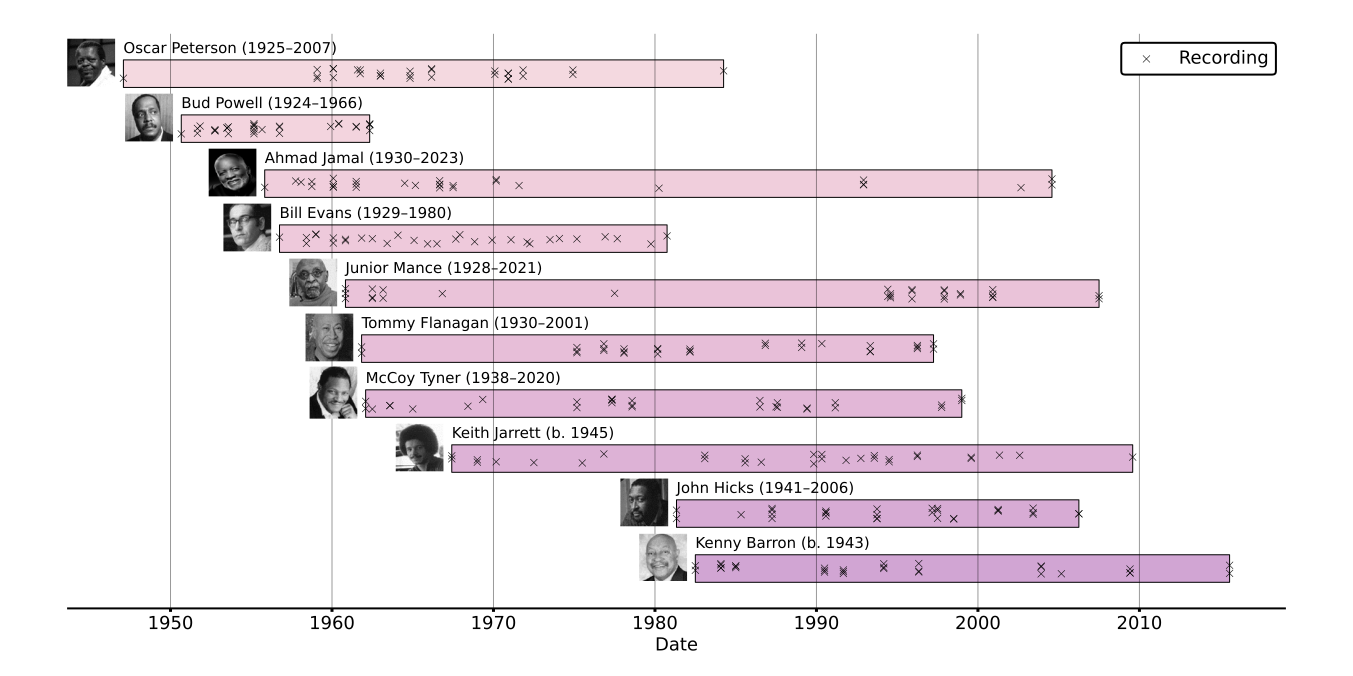
\includegraphics[width=0.9\textwidth]{figures/jtd/figure_1.png}
  \caption[Process followed for constructing JTD.]{Process followed for constructing JTD. Arrow block symbols indicate stages where tracks/artists may be removed.}
\label{fig:jtd_construction}
\end{figure}

When compiling any database of music recordings, deciding which material to include can be challenging. To simplify the process, we first identified a body of suitable ensembles, and then identified appropriate recordings from their discography to include in JTD. Our database curation and annotation procedure is shown in Figure \ref{fig:jtd_construction}.

\subsection{Performer Selection}

The criteria used to decide whether an artist should be included in \GLS{JTD} was that they should be both ``popular'' and ``prolific''. With relation to ``popularity'', we wanted to ensure that artists would only be included if they were both representative of general jazz listening habits and were highly regarded by experts. With relation to ``prolificacy'', we wanted to ensure that artists would only be included if they had recorded a significant amount of material in the piano-bass-drums trio format.

\subsubsection{Identifying ``Popular'' Performers}

We searched the Last.fm platform to obtain an overview of jazz listening habits. Last.fm is an online recommendation service that allows users to build profiles of their personal taste by tracking the music they listen to across many streaming platforms. We scraped the names of the top 250,000 performers and groups on Last.fm most frequently tagged by users with the genre ``Jazz'', using their official API.\footnote{\url{https://www.last.fm/api}} We ordered by tag count, rather than by plays or favorites, as we wanted to find the most quintessentially ``jazz'' artists, rather than those who fused jazz with other styles. 

\begin{figure}[t!]
  \centering
  \includesvg[width=0.75\textwidth]{figures/jtd/figure_2}
  \caption[Total streams (``scrobbles'') of all recordings made by the top 20 ``trio'' artists most-frequently tagged as ``Jazz'' on Last.fm.]{Total streams (``scrobbles'') of all recordings made by the top 20 ``trio'' artists most-frequently tagged as ``Jazz'' on Last.fm.}
\label{fig:jtd_total_streams}
\end{figure}

From the resulting list of performers and groups, we selected only those with the word ``Trio'' in their name. This left 249 unique performers or groups. While the names of many of the ``usual suspects'' featured prominently in this list (e.g., Bill Evans, Keith Jarrett), it also included several performers that were mainly known in other genres (e.g., Dee Felice, who accompanied soul singer James Brown when he performed jazz standards) or that mostly composed soundtrack or ``stock'' music (e.g., Vince Guaraldi, famous for the soundtrack to ``A Charlie Brown Christmas'': see Figure \ref{fig:jtd_total_streams}).

We then cross-referenced the Last.fm results against two major jazz textbooks, keeping only those artists that received a mention in the discographies of either Ted Gioia's ``The History of Jazz'' \citeyearpar{Gioia2011} or Mark Levine's ``The Jazz Piano Book'' \citeyearpar{Levine2011}. The intention here was to capture artists regarded highly by jazz experts. We note, however, that the retrospective nature of these textbooks could have meant that performers who have become active only in recent years (or, indeed, in the time since their publication) were excluded; future revisions of \GLS{JTD} may use subsequent editions of both textbooks. 

This narrowed the total number of groups to 33, all of which were named after a single musician (e.g., the Oscar Peterson Trio). This musician would have led the ensemble and typically composed the majority of the compositions they would play. Two bandleaders were bassists (Dave Holland and Ray Brown) and the remainder were pianists; no bandleaders were drummers.

\subsubsection{Identifying ``Prolific'' Performers}

Next, we turned to searching the MusicBrainz service to acquire a more detailed summary of each bandleader's recorded discography. MusicBrainz is a community-driven service that provides a comprehensive and open index of discographical metadata (including artist names, recording locations, and release dates) and is commonly used in music information retrieval tasks. We scraped MusicBrainz using their API to gather metadata relating to every individual recording ever made by each of our 33 bandleaders.\footnote{\url{https://musicbrainz.org/doc/MusicBrainz_API}} This resulted in the identification of 18,504 recordings.

We removed recordings that (1) were duplicated across several releases (for instance, those that also appeared on compilation albums), (2) did not contain a complete trio lineup, or that included multiple musicians performing on one instrument (for example, a piano ``four hands'' recording), (3) featured a musician doubling on a second instrument (for instance, a pianist who also played synthesizer, or a drummer who played auxiliary percussion), and (4) contained keywords in their title that suggested that they were incomplete performances (e.g., ``breakdown'', ``outtake'', ``false start'').

Four of the 33 bandleaders recorded less than an hour of material in the trio setting; amongst these, Dave Brubeck, Count Basie and Joe Zawinul were all better known for their work leading larger ensembles, while Art Tatum worked mainly in a trio of piano, bass, and guitar. After omitting the recordings by these bandleaders, 4,659 tracks remained.

\subsection{Recording Selection}

\subsubsection{Inclusion Criteria}\label{sec:jtd_inclusion_criteria}

To obtain a consistent set of tracks that could be analyzed reliably by our automated pipeline, we defined inclusion criteria to compare each recording against before including it in JTD. A track must have had: (1) an approximate tempo between 100 and 300 quarter-note beats-per-minute (BPM), assessed by tapping along to the opening measures of the performance, (2) a clear quarter note pulse, with a time signature of either three or four beats per measure (and with no changes in meter), (3) an identifiable piano solo, accompanied by bass and drums with no interruptions in the ensemble texture (i.e., ``solo breaks''), (4) an uninterrupted ``swing eighths'' rhythmic feel, and (5) a link to the recording on YouTube.

Additional criteria were specified for each instrument in the trio. During their solo, pianists must have played on acoustic instruments (rather than, e.g., synthesizer or ``Rhodes'' piano), and without any external FX (e.g., reverb, distortion). Bassists must also have played on an unmanipulated acoustic instrument using their fingers or a plectrum, not a bow. Drummers must have used a traditional ``traps'' kit (snare and kick drums; multiple cymbals, including hi-hat, ride, and crash; tom-toms), without auxiliary percussion (e.g., shakers, maracas). This must also have been played using sticks, rather than wire brushes or cloth mallets. 

These requirements were included so as to (1) ensure that all notes had clear onset times, and (2) maximize the acoustic similarity between the recordings in the dataset and the distribution of (pop, rock) material typically used to train audio source separation models. 

\subsubsection{Metadata Curation}\label{sec:jtd_metadata_curation}

For the recordings that met the inclusion criteria, we combined the metadata scraped from MusicBrainz with additional fields compiled manually, including timestamps for the beginning and ending of the piano solo, the position of individual instrument sources across the stereo spectrum, and the time signature. YouTube URLs were scraped from the ListenBrainz service using the track identifiers returned from MusicBrainz and manually corrected in the case of any false positives. Audio was downloaded from the URLs, trimmed to the piano solo, and stored in a lossless format with a sample rate of 44.1 kHz.

We elected only to include audio from piano solos as this is typically the only section in a performance where every musician would be expected to improvise. For instance, in the ``head'' (melodic statements that occur at the beginning and ending of ``straight ahead'' jazz performances), the material is pre-composed; while, in bass or drum solos, the accompanying musicians may choose not to play \citep{Monson1996}.

\begin{figure}[t!]
  \centering
  \includesvg[width=0.75\textwidth]{figures/jtd/figure_3}
  \caption[Duration of piano solo excerpts by all bandleaders.]{Duration of piano solo excerpts by all bandleaders. Bar colour indicates subset (either \GLS{JTD} or JTD-300).}
\label{fig:jtd_solo_durations}
\end{figure}

Of the 4,659 recordings that were evaluated, 1,294 (27.8\%) were included in JTD. The combined duration of all piano solos in these recordings was 44.5 hours (Figure \ref{fig:jtd_solo_durations}). These recordings were made between 1947 and 2015, with a median recording year of 1972. The vast majority (93\%) had a time signature of four beats per measure.

\begin{figure}[t!]
  \centering
  \includesvg[width=0.75\textwidth]{figures/jtd/figure_4}
  \caption[Number of tracks featuring the 10 performers on each instrument with the most recordings in \GLS{JTD}.]{Number of tracks featuring the 10 performers on each instrument with the most recordings in \GLS{JTD}.}
\label{fig:jtd_tracks_by_performer}
\end{figure}

The recordings in \GLS{JTD} featured 34 different pianists, 98 bassists, and 106 drummers. Bassist Ray Brown and drummer Ed Thigpen performed together as a rhythm section on the largest number of individual recordings (94). Of those who were not also the leader of their own trio, bassists Ron Carter and Sam Jones accompanied the largest number of different pianists (7), while drummer Roy Haynes accompanied 6 pianists. Figure \ref{fig:jtd_tracks_by_performer} shows the number of tracks by the ten performers on each instrument with the greatest number of recordings in JTD.

\subsubsection{JTD-Brushes}

Excluding recordings where the drummer used wire brushes resulted in the removal of 973 tracks scraped from MusicBrainz. To address this imbalance, we created a separate set of annotations for tracks that were only rejected from \GLS{JTD} because of the use of brushes. We define this related database as JTD-Brushes. Note that the recordings in JTD-Brushes were not curated to the same extent as those in JTD; the full recording was used, rather than only the piano solo, and the time signature was estimated by the beat tracker automatically, rather than being provided beforehand. The duration of the recordings in JTD-Brushes was 79 hours. While the remainder of this article focuses on the curated JTD, we envisage that JTD-Brushes may be of use in developing or evaluating e.g., beat tracking or ``soft'' onset detection models \citep[e.g., ][]{Tomczak2023} that can cope with a broader variety of drumming techniques.

\subsection{Class Imbalance}\label{sec:jtd_class_imbalance}

A side effect of our inclusion criteria was that bandleaders who worked most frequently in the acoustic ``swing'' style were overrepresented in the JTD. Conversely, those who worked across a variety of styles or who frequently incorporated electronic elements into their music had very few recordings that met the inclusion criteria. The three bandleaders with the most audio in the \GLS{JTD} were Bill Evans (5.5 hours), Keith Jarrett (4), and Oscar Peterson (3.5). Meanwhile, Abdullah Ibrahim, Brad Mehldau, and Dave Holland were each represented in the \GLS{JTD} by less than half an hour of audio.

This class imbalance could prove problematic were predictive models to be trained on the JTD. To that end, we created a subset of \GLS{JTD} (defined as JTD-300), that includes an equal number of recordings from the ten bandleaders with the most audio in JTD, sampled chronologically across the duration of their careers. Together, recordings led by these ten musicians --- all of whom were pianists --- made up 62.6\% of the total duration of audio in \GLS{JTD} (see Figure \ref{fig:jtd_solo_durations}).

For each of these bandleaders, we sorted their tracks in \GLS{JTD} chronologically by the date of recording. In cases where a full date could not be obtained from MusicBrainz, a track was estimated to have been made either midway through the month (in cases where both a month and year were given) or year (when only a year was given) it was recorded. In cases where multiple dates were given for one track (i.e., when an album was recorded over a period of time, without dates being assigned to individual tracks), we took the midpoint of these dates. If no dates were provided at all, the track was excluded from selection.

\begin{figure}[]
  \centering
  \includesvg[width=1.0\textwidth]{figures/rsos_rhythm/figure_1}
  \caption[Duration of the recording career for each of the ten pianists included in \GLS{JTD-300}]{Duration of the recording career for each of the ten pianists included in \GLS{JTD-300}. Markers indicate the date of recordings that appear in \GLS{JTD-300}, randomly jittered horizontally and vertically for visual clarity.}
\label{fig:rsos_jtd300}
\end{figure}

\begin{figure}[]
  \centering
  \includesvg[width=1.0\textwidth]{figures/rsos_rhythm/figure_s1}
  \caption[Durations of recordings in \GLS{JTD-300}.]{Durations of recordings in \GLS{JTD-300}. Each column shows the total duration of the recordings by every bandleader with recordings in \GLS{JTD-300}, with the green proportion corresponding with those tracks that are included within each subset (shown also as a percentage along the columns).}
\label{fig:rsos_bandleader_proportions}
\end{figure}

Next, we sorted each track into one of 30 equally spaced bins; the left edge of the first bin coincided with the date of a bandleader's earliest recording, and the right edge of the final bin with the day of their final (or most recent) recording. Tracks were ordered within each bin by the proximity of their recording date to the midpoint of that bin; if multiple recordings were made on the same day, they were arranged following the order in which they appeared on their original release. We then included the first track from each bin in JTD-300: in cases where a bin was empty, we added an additional track from the first bin, then the second bin, and so on, until 30 tracks were obtained for each bandleader (Figure \ref{fig:rsos_jtd300}). We show the proportion of recordings by each bandleader contained in JTD-300 within Figure \ref{fig:rsos_bandleader_proportions}.

\begin{figure}[t!]
  \centering
  \includesvg[width=0.75\textwidth]{figures/jtd/figure_5}
  \caption[Histogram grouping number of tracks in \GLS{JTD} by year of recording.]{Histogram grouping number of tracks in \GLS{JTD} by year of recording. Bar colour indicates subset (\GLS{JTD} or \GLS{JTD-300}.}
\label{fig:jtd_tracks_by_year}
\end{figure}

The combined duration of the audio in JTD-300 was 11.75 hours (26.4\% of the duration of JTD). As with JTD, these recordings were made between 1947 and 2015, with a median recording year of 1977.5. The distribution of recording years included in JTD-300 was comparable with \GLS{JTD} (Figure \ref{fig:jtd_tracks_by_year}). 95\% of JTD-300 recordings had a time signature of four beats per measure. We envisage that JTD-300 will most likely be of use in performer identification tasks or analyses of chronological trends in improvisation practice (here, see Chapter \ref{chap:rhythm_rsos}). Tasks that do not require balanced class sizes may be better accomplished using the full JTD.

\section{Annotation}

\subsection{Source Separation}

\subsubsection{Audio Channel Selection}

Before the development of full-spectrum stereophonic panning in the 1970s, audio signals could only be panned to the left or right speaker output, or both (center channel). For tracks in the \GLS{JTD} where at least one instrument in the trio was hard-panned in this manner (39\%), source separation was applied independently to the left and right monaural signals alongside the center output. The required channel was identified manually for each instrument during the metadata curation process (see section \ref{sec:jtd_metadata_curation}).

\subsubsection{Model Selection}

The \texttt{ZFTurbo} audio source separation model \citep{Solovyev2024} was used to separate each track in the \GLS{JTD} into four sources; ``bass'', ``drums'', ``vocals'', and ``other'' This model combines three existing source separation models and achieved the first prize in a recent community sound demixing competition \citep{Fabbro2024}. 

\subsubsection{Audio Preprocessing}\label{sec:jtd_audio_preprocessing}

As the \texttt{ZFTurbo} model was not trained explicitly to separate piano audio, we used the ``other'' source (consisting of the residual audio after removing every other source from the mixed signal) for this instrument. This meant it was possible that audio from the bass and drums could have ``bled'' into this track, which would have affected the performance of our downstream annotation pipeline.

To mitigate this possibility, prior to annotation we filtered the ``other'' source using a second-order Butterworth bandpass filter. Our goal was to attenuate frequency bands that could also be occupied by the drums and bass, while minimizing any damage to the quality of the piano audio. The filter was set to attenuate frequencies outside the range of 55--3520 Hz, equivalent to a six-octave span from $A_1$--$A_7$: as shown in Edwards et al. \citeyearpar{Edwards2023}, the vast majority of note events in jazz piano performance typically fall within this range. 

We demonstrate in section \ref{sec:jtd_alternate_methods} that filtering the piano audio improved the accuracy of our onset annotation pipeline compared to using the raw audio, and that this particular frequency range performed better than an alternative, quantitatively ``narrower'' range.

\subsubsection{``Vocal'' Source}

Another possibility was that the unmixed ``vocal'' source could also contain piano audio, which would necessitate summing it with the ``other'' source. We manually inspected the ``vocal'' source across a sample of 34 recordings sampled from JTD-300 (see section \ref{sec:jtd_ground_truth_annotations}). In all of these cases, the ``vocal'' source was either silent or contained vocalizations of the musicians (or, occasionally in the case of a live recording, members of the audience) reacting to the performance. Therefore, the ``vocal'' source was not used for downstream data extraction.

\subsection{Data Extraction}

Our data extraction pipeline consisted of three components: (1) an onset detection algorithm, applied to each separated audio source (except ``vocal''), (2) a beat and downbeat tracking algorithm, applied to the raw audio mixture, and (3) an algorithm to match onsets with their nearest beat, in order to assign a metrical interpretation to each onset. Our implementations of (1) and (2) were from the \texttt{madmom} (version \texttt{0.17.0}) Python package \citep{Bock2016}. The default setting of 100 frames per second was used in \texttt{madmom}, such that near-simultaneous events with a time difference of less than one frame (likely including, e.g., piano chords) would be treated as a single onset.

\subsubsection{Onset Detection}\label{sec:jtd_onset_detection}

The \texttt{CNNOnsetDetector} function in \texttt{madmom} was used to detect onsets in the isolated audio obtained for each instrument in the trio. This algorithm came first in the most recent \texttt{MIREX} onset detection competition.\footnote{\url{https://nema.lis.illinois.edu/nema_out/mirex2018/results/aod/}\label{note:mirex_2018}} A convolutional neural network (\GLS{CNN}) is fed spectrogram frames of audio (at the default rate of 100 frames per second) to obtain an onset activation function; this envelope is then smoothed using a moving window and onsets are identified as local maxima higher than a predetermined threshold. Both the window size and the peak-picking thresholds were optimized separately for each instrument class in \GLS{JTD} (see section \ref{sec:jtd_validation_results}). In section \ref{sec:jtd_alternate_methods}, we demonstrate that, for detecting onsets in the \GLS{JTD} piano audio, this algorithm outperformed both an existing automatic piano transcription algorithm \citep{Kong2021} and a naive spectral flux approach.

\subsubsection{Beat Detection}\label{sec:jtd_beat_detection}

The \texttt{DBNDownBeatTracker} function in \texttt{madmom} was used to detect the position of quarter note beats and downbeats in the audio mixture. This algorithm came first in the most recent \texttt{MIREX} beat tracking competition.\footnote{\url{https://nema.lis.illinois.edu/nema_out/mirex2019/results/abt/smc/}} A recurrent neural network (\GLS{RNN}) is applied to frames from an audio spectrogram to distinguish between beats, downbeats, and non-beat classes; a dynamic Bayesian network (\GLS{DBN}) then infers meter from the RNN observations (using the default rate of 100 frames per second). Meter changes cannot be detected by this algorithm, which led us to incorporate this into our inclusion criteria (see section \ref{sec:jtd_inclusion_criteria}).\footnote{\citet{Foscarin2024} have since proposed an end-to-end algorithm that does not require \GLS{DBN} post-processing of an activation function, which alleviates constraints on meter while potentially leading to greater overall precision. This was not available at the time \GLS{JTD} was compiled, however.}

We applied this algorithm multiple times to a single track. First, the default parameters specified by the authors were used, with the tempo allowed to vary between 100 and 300 quarter note beats-per-minute (as specified in the inclusion criteria). This resulted in the timestamps changing tempo frequently, due to the lack of constraint in the parameter settings. 

To resolve this, we gradually reduced the range of permissible tempo values for the beat tracker over a number of iterations. First, we calculate the durations between successive beats as
\begin{align}
d_{i} = b_{i+1} - b_{i}, \ i = 1, 2, \dots, n-1, 
\end{align}
where $n$ is the total number of beats in the track. Then, we calculate the inter-quartile range of beat durations $IQR_d$ as
\begin{align}
IQR_d &= Q_3\left( \{d_1, d_2, \dots, d_{n-1}\} \right) - Q_1\left( \{d_1, d_2, \dots, d_{n-1}\} \right),
\end{align}
and use this to filter the initial durations $d$ where 
\begin{align}
d'_i &= \{ Q_1 - 1.5(IQR_d) \leq d_i \leq Q_3 + 1.5(IQR_d) \}, \ i = 1, 2, \dots, n-1.
\end{align}
Finally, we recalculate $Q_1$ and $Q_3$ using only values of $d'$ and set these as the new minimum and maximum tempo for the beat tracker in the next iteration of the process. The total number of iterations this process ran for was optimized for the recordings in \GLS{JTD} (see section \ref{sec:jtd_validation}).

The downbeat classes estimated from the RNN were then combined with the detected beat positions and the time signature for the recording in order to assign measure numbers to every detected timestamp. 

\subsubsection{Beat-Onset Matching}\label{sec:jtd_beat_onset_matching}

The final stage of our detection pipeline involved matching every beat with the nearest onset detected in each instrumental source. The size of the window used to match any given onset to the nearest beat varied depending on the tempo of a track. Onsets played up to one thirty-second note before and one sixteenth note after any given timestamp were included within the window; whichever onset had the smallest absolute distance to the beat was understood to mark the pulse. If no onsets were contained within a window, then the musician was considered to not have marked the pulse at that timestamp. 

Our rationale for using an asymmetric window came from previous research which has suggested that jazz soloists are more likely to ``lag behind'' and mark the beat later than their rhythm section, as opposed to earlier \citep{Butterfield2010}. Additionally, \citet{Corcoran2021} describe how notes played more than a thirty-second note earlier than a given beat act as a subdivision of the previous beat (i.e., a delayed, swung ``eighth'' note), as opposed to marking that beat itself. 

\subsection{Validation}\label{sec:jtd_validation}

\subsubsection{Ground Truth Annotations}\label{sec:jtd_ground_truth_annotations}

To evaluate the effectiveness of our annotation pipeline, we manually annotated beat, downbeat, and onset positions across a representative subsample of tracks. In particular, we wanted to check whether the pipeline was resilient to a range of possible recording qualities, and also to the styles of the musicians represented most prominently in JTD. Consequently, we adopted a systematic approach, annotating the earliest, middle, and final recordings made by each of the ten bandleaders in JTD-300. Owing to his overrepresentation in JTD, we also annotated an additional four tracks by Bill Evans (selected randomly from JTD-300) --- enough to ensure that the percentage of recordings led by Evans in the subsample (20.6\%) was equivalent to \GLS{JTD} (19.6\%).

Two of the authors and one research assistant created the reference annotation set. The annotations of the assistant were checked for consistency by the lead author. The combined duration of the 34 recordings in the subsample was 72 minutes. The median recording year was 1975, comparable with both \GLS{JTD} and JTD-300 (see sections \ref{sec:jtd_metadata_curation} and \ref{sec:jtd_class_imbalance}), and the range of recording years was identical (1947--2015). 88\% of recordings had a time signature of 4 quarter notes per measure. 

\subsubsection{Validation Results}\label{sec:jtd_validation_results}

The performance of the pipeline was determined by considering the proportion of detected annotations that occurred within a 50 ms window of a ground truth annotation. For every track in the subsample, separate precision, recall, and $F$-measures were computed for each class: (1--3) the onsets within each unmixed instrumental source, and (4) the quarter note beats and (5) downbeats within the audio mixture. When $F = 1.0$, every onset or beat detected by the pipeline could be matched with a ground truth annotation, with no onsets or beats unmatched. 

We applied the gradient-free, nonlinear optimization algorithm \texttt{subplex} \citep{Rowan1990} implemented in the \texttt{NLopt} (version \texttt{2.7.1}) Python package to set the parameters of the beat and onset detection algorithms separately for each audio source.\footnote{\url{https://github.com/stevengj/nlopt}} In every case, the mean value of $F$ across the entire hand-annotated subsample was treated as the objective function to maximize. Note that, for the beat detection algorithm, only the $F$-measure obtained from evaluating the beat timestamps --- not the downbeats --- was considered during optimization.

\begin{table}[h!]
\centering
\caption[Optimized results for onset detection per instrument]{Optimized results for onset detection per instrument, showing mean $F$-measure, precision, and recall. Brackets show \emph{SD}s.}
\label{tab:jtd_optimization_results}
\begin{tabular}{l c c c c c c}
\toprule
 & \textbf{Piano} & \textbf{Bass} & \textbf{Drums} & \textbf{Beats} & \textbf{Downbeats} \\
\midrule
\textbf{F-measure} & 0.93 (0.03) & 0.93 (0.05) & 0.95 (0.03) & 0.97 (0.05) & 0.63 (0.44) \\
\textbf{Precision} & 0.93 (0.04) & 0.94 (0.04) & 0.96 (0.04) & 0.97 (0.05) & 0.63 (0.44) \\
\textbf{Recall} & 0.93 (0.04) & 0.93 (0.07) & 0.94 (0.04) & 0.97 (0.05) & 0.63 (0.44) \\
\bottomrule
\end{tabular}
\end{table}

The values of $F$ obtained from the optimized parameter set are shown in Table \ref{tab:jtd_optimization_results}. The performance of the onset detection algorithm was broadly equivalent across instrument classes, with drums performing marginally better than bass and piano. In comparison with earlier results obtained from applying the same algorithm to equivalent multi-tracked audio datasets (``polyphonic pitched'', $mean(F) = 0.95$, ``plucked strings'', $mean(F) = 0.90$, ``solo drums'', $mean(F) = 0.93$, see note \ref{note:mirex_2018}), we obtained similar onset detection accuracy. This indicated to us that the source separation process was unlikely to have caused significant damage (in the form of artifacts, etc.) to the audio, to the point that onset detection algorithms trained on multi-tracked recordings could not also be applied to JTD.

While the beat tracking results indicated good performance, downbeat tracking was noticeably worse. To understand why, we inspected all tracks where $F(downbeat) = 0.0$, while $F(beat) > 0.95$ (i.e., the downbeats were out-of-phase). We observed that, in the majority of these cases, metrically ``strong'' beats were being mistaken for other ``strong'' beats (i.e., beat 2 and beat 4, in 4/4), rather than ``weak'' beats, and vice versa. This suggests that our results may still have some value in the analysis of metrical structure, and we also observed that our results were in line with those obtained from applying the same algorithm to other metrically complex forms of music.\footnote{\url{https://www.music-ir.org/mirex/wiki/2016:Audio_Downbeat_Estimation_Results}} However, future revisions of \GLS{JTD} may leverage the modular design of our codebase to integrate more sophisticated downbeat tracking algorithms \citep[e.g.,][]{Foscarin2024} as these become available.

Finally, we looked at the temporal difference between equivalent automatic and ground truth annotations. The pipeline tended to annotate beats and onsets earlier than the human annotators did; the mean difference in beat location time (algorithm--human) was $-4.82$ ms ($SD = 4.58$), and for onsets the mean difference was $-4.53$ ms ($SD = 3.42$). There were no substantial differences between onsets detected for different instrument classes here (piano, $-5.77$ ms, bass: $-4.29$ ms, drums: $-4.53$ ms). In context, this variation was likely perceptually sub-threshold, and should be negligible in most applications.

\subsubsection{Alternative Methods}\label{sec:jtd_alternate_methods}

Next, we compared several alternative onset detection methods, using the piano audio and corresponding ground truth annotations for evaluation. These methods were: (1) an automatic transcription model \citep{Kong2021}, which generates MIDI (incorporating both pitch and rhythmic information) from audio, (2) a naive audio signal processing approach, whereby onsets were identified as local maxima from a normalized spectral flux envelope, using the implementation from the \texttt{librosa} (version \texttt{0.8.1}) Python package \citep{McFee2015}, (3) the current approach, without the audio filtering described in section \ref{sec:jtd_audio_preprocessing}, and (4) the current approach, with a quantitatively ``narrower'' bandpass filter (attenuating frequencies outside the range of 110--1760 Hz i.e., $A_2$--$A_6$).

Note that, as method (1) generates multiple MIDI events for what would be regarded perceptually as a single onset (i.e., a chord), near-simultaneous MIDI events within a window of 50 ms were grouped together, with the onset of the earliest event taken as the onset of the whole group. The size of this window was optimized following the method described in \ref{sec:jtd_validation_results}, as were the individual parameter sets used to pick peaks from the activation functions returned separately from methods (2--4). The default setting of 100 frames per second was used for method (1).

\begin{table}[h!]
\caption[Onset detection results per method, piano only]{Onset detection results per method, piano only}
\label{tab:jtd_methods_comparison}
\centering
\begin{tabular}{l c c c c}
\toprule
 & \textbf{(1)} & \textbf{(2)} & \textbf{(3)} & \textbf{(4)} \\
\midrule
\textbf{F-measure} & 0.77 (0.13) & 0.84 (0.06) & 0.92 (0.03) & 0.92 (0.03) \\
\textbf{Precision} & 0.71 (0.16) & 0.79 (0.10) & 0.90 (0.06) & 0.95 (0.03) \\
\textbf{Recall} & 0.86 (0.09) & 0.90 (0.04) & 0.93 (0.03) & 0.89 (0.05) \\
\bottomrule
\end{tabular}
\end{table}

The results from this comparison are given in Table \ref{tab:jtd_methods_comparison}. For detecting onsets in the \GLS{JTD} piano audio, the current approach outperformed all four alternatives. In particular, we noted how ``narrowing'' the bandpass filter seemed to affect the precision-recall tradeoff of the CNN predictions: the narrower filter setting (4), for example, resulted in a lower false positive rate than the settings described in \ref{sec:jtd_audio_preprocessing}, but a higher false negative rate. The current approach, with filter settings between those of methods (3--4), resulted in approximately equal precision and recall. All three CNN-based methods significantly outperformed spectral flux.

The results obtained for method (1) were disappointing, especially when compared to those given by the authors. One possibility was that this model may have overfitted to the acoustic properties of the instrument(s) in its training data and be less resilient to the varied recording conditions contained in JTD. More robust approaches that make use of e.g., augmented training data may be worth exploring \citep[here, see][]{Edwards2024}.

Regardless, these MIDI annotations are included in JTD, with the caveat that they may be of greater use in downstream tasks which do not require strict timing accuracy (e.g., in analyzing melodic or harmonic content). The total number of MIDI events was 2,174,833 ($\sim2.5$x the number of total piano onsets).

\subsubsection{Bass Annotation}\label{sec:jtd_bass_detection}

Considering the results in Table \ref{tab:jtd_optimization_results}, the somewhat higher standard deviation of bass onset detection results suggests that there may have been a subset of onset types that gave outlier results, diminishing the overall accuracy of the pipeline. While we could not investigate every possibility, we could check three hypotheses: whether bass annotation was negatively affected (1) by if a bass note was ``raked'', (2) by if both bass and drums played simultaneously, and (3) on specific beats of the bar.

For hypothesis (1), we defined a ``rake'' as a technique in jazz bass where the finger is dragged from one string to the next lower string. We collected all groups of three bass onsets that were immediately preceded and then followed by a single onset that could be matched with the quarter-note pulse. Searching all tracks with ground truth annotations, we found 57 occurrences of this pattern, equivalent to 285 onsets. 

For each track where this pattern occurred at least once, we computed the $F$-measure between all of the automatically detected ``rake'' patterns and ground truth onsets located within the span of each ``rake'' (allowing for a tolerance of 50 ms). From this analysis, $mean(F) = 0.91$ ($SD = 0.08$) --- i.e., close to the value in Table \ref{tab:jtd_optimization_results}. This suggests that whether a bass note was ``raked'' did not have a substantial impact on the accuracy of the detection pipeline.

For hypothesis (2), we collected all automatically detected bass onsets that were matched with a timestamp from the beat tracker, provided that a drum onset could also be matched with that same timestamp ($N = 10,538$). The equivalent ground truth annotations were collected and, again, $mean(F)$ was computed only for these annotations. In this case, $mean(F) = 0.92\;(SD = 0.06)$) --- again, nearly identical to the value obtained using all annotations. This led us to conclude that accuracy of onset detection was not substantially lower when both bass and drums played together on the same beat.

Finally, for hypothesis (3), we collected automatic and manual onset annotations matched with each individual beat of the ground truth metre annotations. $F$-scores then were computed for each individual beat (i.e., comparing all known beat 1s, all beat 2s, etc.) across every track. Here, $mean(F_{B1}) = 0.94\;(SD=0.07)$, $mean(F_{B2}) = 0.94\;(SD=0.12)$, $mean(F_{B3}) = 0.95\;(SD=0.06)$, and $mean(F_{B4}) = 0.95\;(SD=0.04)$. All results are again in line with Table \ref{tab:jtd_optimization_results}, which suggests that there was no evidence that outlying results occurred systematically on individual beats of the bar.

\section{Analysis}

Across JTD, there were 2,206,413 onsets (piano: 866,116, bass: 543,693, drums: 796,604) and 512,272 beat timestamps, 130,547 of which were labeled as downbeats. On average, a solo contained 669 piano onsets, 420 bass onsets, 616 drums onsets, 396 beats, and 101 downbeats. 87.4\% of beat timestamps could be matched to a drum onset, and 82.0\% matched to a bass onset; only 71.0\% of beats could be matched to a piano onset, which underlines that keeping time is not the primary aim of jazz soloists.

\subsection{Solo Duration}

On average, the duration of a piano solo in \GLS{JTD} was 2 minutes and 3 seconds. Both the shortest and longest solos were by Bud Powell, with the shortest lasting only 22 seconds (``Salt Peanuts'', \citeyear{Powell1956}), and the longest 7 minutes, 17 seconds (``Reets And I'', \citeyear{Powell1962}).

\begin{figure}[t!]
  \centering
  \includesvg[width=0.75\textwidth]{figures/jtd/figure_6}
  \caption[Mean duration of solos by different \GLS{JTD} pianists.]{Mean duration of solos by different \GLS{JTD} pianists. Error bars show standard errors.}
\label{fig:jtd_mean_track_duration_by_pianist}
\end{figure}

There was considerable variation in the duration of solos played by different pianists (Figure \ref{fig:jtd_mean_track_duration_by_pianist}). In particular, the later a pianist's first recording in \GLS{JTD} was made (i.e., the later they began their career), the longer they tended to solo for. For the 9 (out of 27) pianists in \GLS{JTD} with the longest average solo durations, the median year their first recording was made was 1967; for the 9 pianists with the shortest solos on average, the median year was 1956. 

One possible explanation is that the open-ended formal designs (e.g., modal ``vamps'', ``time, no changes'') that became popular in jazz during the latter half of the twentieth century proved more suitable for extended improvisation, as this did not need to follow the harmonic structure of an underlying ``song form'' \citep{Gioia2011}. Changing trends in the music business could provide another explanation; up until the mid-1950s, record companies would often fill albums with multiple shorter recordings rather than longer individual takes, so that individual tracks could be released as singles to be played on jukeboxes and radio stations \citep{Priestley1991}.

\subsection{Tempo}\label{sec:jtd_tempo}

Rather than working directly with the timestamps estimated from the beat tracker, we instead defined the location of a ``beat'' as the mean of all onsets matched to a single timestamp (see section \ref{sec:jtd_beat_onset_matching}). Given our omission of tracks with, e.g. a predominant ``two-beat'' feel (where half notes could conceivably be understood to mark the ``beat'') and with ``straight'' eighths (where these could be felt to mark the beat), these timestamps would be expected to correspond with quarter notes. In cases where fewer than two onsets were matched with a single timestamp (for instance, where at least two instruments played ``off'' that beat), it was set to missing. At least two instruments played ``on'' the beat for 88.7\% of detected beat timestamps within JTD.

\begin{figure}[t!]
  \centering
  \includesvg[width=0.75\textwidth]{figures/jtd/figure_7}
  \caption[Distribution of tempi in \GLS{JTD}.]{Distribution of tempi in \GLS{JTD}, shown in quarter note beats-per-minute).}
\label{fig:jtd_mean_tempo}
\end{figure}

The mean tempo $\bar{y}$ of a recording in beats-per-minute was calculated as 
\begin{align}\label{eq:mean_tempo}
\bar{y} = \dfrac{\sum_{i=1}^N\frac{60}{x_i - x_{i-1}}}{N-1}
\end{align}
where $x_i$ is the mean of all onsets matched to beat $i$, for $i \geq 1$. Across \GLS{JTD}, the observed $mean(\bar{y}) = 193.92 \ \text{BPM}$ ($SD = 46.93$, Figure \ref{fig:jtd_mean_tempo}); this was comparable to the equivalent result calculated using the timestamps $y'$ estimated from the beat tracking algorithm ($mean(\bar{y'}) = 193.70, SD = 46.59$). The slowest performance in \GLS{JTD} had a mean tempo of 102.10 BPM (Cedar Walton, ``Ghost of a Chance'', \citeyear{Walton2010}) and the fastest 299.82 BPM (John Hicks, ``Airegin'', \citeyear{Hicks1987}).

As a measure of tempo stability, for each track we obtained the standard deviation of the tempo normalized by the mean tempo i.e., the percentage fluctuation about the overall tempo (``tempo fluctuation'', $F$). This can be written simply as
\begin{align}\label{eq:tempo_fluctuation}
F = \dfrac{\sqrt{\frac{1}{N-1} \sum_{i=1}^N (y_i - \bar{y})^2}}{\bar{y}},
\end{align}
where $y_i$ is the tempo value in quarter-note beats-per-minute at beat $i$. The observed $mean(F) = 5.55\%$ ($SD = 2.70$) for \GLS{JTD} recordings, suggesting that they were generally stable.

We also calculated the slope of a linear regression of instantaneous tempo against beat onset time (``tempo slope'', $S$) using the standard least squares formula
\begin{align}\label{eq:tempo_slope}
S = \frac{\sum_{i=1}^N (x_i - \bar{x}) (y_i - \bar{y})}{\sum_{i=1}^N (x_i - \bar{x})^2},
\end{align}
such that $S > 0$ implies acceleration and $S < 0$ implies deceleration. The observed $mean(S) = 0.04\ \text{BPM/s}$ ($SD = 0.10$) for \GLS{JTD} recordings, suggesting that they displayed a very slight tendency towards acceleration (with a predicted increase of 1 BPM every 25 seconds).

There was no correlation between signed tempo slope and unsigned tempo fluctuation, $r_{S, F}(1292) = -0.06, p = 0.06$; however, there was a positive correlation between the unsigned slope (i.e., any global change in tempo, regardless of direction) and fluctuation, $r_{|S|, F}(1292) = 0.37, p < .001$. There were positive correlations between both mean tempo and signed tempo slope, $r_{\bar{y}, S}(1292) = 0.25, p < .001$, mean tempo and unsigned slope, $r_{\bar{y}, |S|}(1292) = 0.60, p < .001$, and mean tempo and fluctuation, $r_{\bar{y}, F}(1292) = 0.24, p < .001$. This suggests that performances which had a faster pace tended to involve a greater magnitude of tempo change than those which were slower, and were also less stable overall.

\subsection{Swing}\label{sec:jtd_swing}

In jazz, swing refers to the division of the pulse into alternating long and short intervals. Expressed in Western notation, the long interval is typically written as a quarter note triplet, and the short as an eighth note triplet. Empirically, swing can be measured by taking the ratio of these long and short durations --- the swing or ``beat-upbeat ratio'' (\GLS{BUR}), commonly expressed in binary logarithmic form in the literature. This can be written simply as
\begin{align}\label{eq:jtd_bur}
log_2(BUR)=log_2\biggl(\frac{t_{a,b}-t_{a}}{t_{b}-t_{a,b}}\biggr),
\end{align}
where $t_a$ is the onset matched with beat $a$, $t_b$ is the onset matched with beat $b$ (i.e., at beat $a + 1$), and $t_{a,b}$ is the single onset between beats $a$ and $b$. For notated ``swung'' eighths, $log_2(BUR) = 1.0$ ($BUR = 2:1$); vice-versa, for ``straight'' eighths (i.e., the equal-equal subdivision of the beat), $log_2(BUR) = 0.0$ ($BUR = 1:1$).

We searched our database for all discrete groupings of three onsets where the first and last had marked the quarter note pulse. The total number of such groupings was 417,278. Following the analysis of the \GLS{WJD} by \citet{Corcoran2021}, we classified ratios above 4:1 ($log_2(BUR) = 2$) and below 1:4 ($log_2(BUR) = -2$) as outliers, which resulted in the exclusion of 2.10\% of these groupings. The final number of beat-upbeat ratios in the dataset was 408,506 (piano: 151,640, bass: 47,115, drums: 209,751).

\subsubsection{Differences in Swing Between Instruments}\label{sec:jtd_differences_in_swing_between_instruments}

To evaluate the differences in swing ratio between the instruments in the trio, we smoothed the distribution of beat-upbeat ratios obtained for each instrument through kernel density estimation (calculating the bandwidth using Silverman's rule-of-thumb). Then, we applied the peak-picking algorithm (using the default parameters) from the \texttt{SciPy} (version \texttt{1.10.1}) Python library \citep{Virtanen2020} to obtain the local maxima of the smoothed curve. Confidence intervals for these peaks were generated by bootstrapping over the results from different bandleaders ($N = 10,000$ replicates).

\begin{sidewaysfigure}[htbp]
  \includesvg[width=1.0\textwidth]{figures/jtd/figure_8}
  \caption[Distribution of $log_2(BUR)$s between instruments across \GLS{JTD}]{Distribution of $log_2(BUR)$s between instruments across \GLS{JTD}, normalized such that the height of the largest bar in each panel is 1. Dotted vertical lines show peaks of the density estimates; straight lines correspond with the musical notation given along the top of the panel.}
\label{fig:jtd_bur_distribution_by_instrument}
\end{sidewaysfigure}

For the piano, we found one peak in the density estimate, corresponding with $log_2(BUR)$ of 0.37 ($BUR = 1.44:1$, 95\% CI: $[0.15, 0.43]$). For the bass, we found two peaks, corresponding with $log_2(BURs)$ of 0.06 ($1.06:1$, $[0.03, 0.13]$) and 1.23 ($3.41:1$, $[1.15, 1.27]$). For the drums, we also found two peaks, at $log_2(BUR) = -0.91$ ($0.40:1$, $[-1.15, -0.70]$) and 1.18 ($3.25:1$, $[1.13, 1.23]$). These density estimates and the corresponding peaks are shown in Figure \ref{fig:jtd_bur_distribution_by_instrument}.

This analysis suggested that (1) all instrument classes primarily targeted long-short divisions of the beat, with the percentage of total $log_2(BURs) > 0.0 = 88.6\%$ (piano: 81.9\%, bass: 89.1\%, drums: 93.4\%); (2) pianist beat-upbeat ratios were closer to notated ``straight'' than ``swung'' eighths, judging by the peak of their density estimate; (3) in contrast, the larger of the two peaks in the bass and drums density estimates suggested that both instruments tended towards higher beat-upbeat ratios than implied by notated swing eighths alone. 

The fact that soloists tended to swing less than the expected $2:1$ ratio --- while accompanists swung ``more'' than this --- has been well documented. Butterfield \citeyearpar{Butterfield2010} has, for instance, suggested that relatively ``straight'' eighth notes helps to maintain forward momentum in a soloist's improvisation, while the more ``swung'' eighth notes of the accompaniment helps to facilitate hierarchical beat perception. We include several examples of sustained ``straight'' ($log_2(BUR) < 0.0$) piano playing in the supplemental materials.

We also noted that the mean beat-upbeat ratio for piano soloists in \GLS{JTD} ($1.53:1$) was close to that obtained for \texttt{SWING} tracks in \GLS{WJD} ($1.41:1$; see Corcoran \& Frieler, \citeyear{Corcoran2021}). Caution should be taken when interpreting these results, however, as \GLS{WJD} contains a greater variety of tempi and solo instruments than JTD.

\subsubsection{Effect of Tempo on Swing}\label{sec:jtd_effect_of_tempo_on_swing}

Next, we considered the relationship between swing and the tempo of a performance. We fitted a linear mixed effects model using the implementation in the \texttt{statsmodels} (version \texttt{0.13.1}) Python library \citep{Seabold2010}, predicting a performer's mean $log_2(BUR)$ using the mean tempo of the recording (standardized through $z$-transformation), their instrument, and the interaction between tempo and instrument as fixed effects (with piano as the reference category). Bandleader was used as a random effect (slopes and intercepts). An individual musician's performance was excluded if 15 ratios could not be obtained, resulting in the exclusion of 471 individual performances out of 3,865 (piano: 30, bass: 401, drums: 40).

\begin{figure}[t!]
  \centering
  \includesvg[width=0.75\textwidth]{figures/jtd/figure_9}
  \caption[Mean $log_2(BUR)$ and tempo for an individual recording and instrument in \GLS{JTD}.]{Mean $log_2(BUR)$ and tempo for an individual recording and instrument in \GLS{JTD}. Solid lines show predictions (without random effects), shaded areas show 95\% confidence intervals (obtained via bootstrapping over data from different pianists, $N = 10,000$)}
\label{fig:jtd_bur_vs_tempo}
\end{figure}

An increase in mean tempo was a significant predictor of a decrease in mean beat-upbeat ratio for a recording (Figure \ref{fig:jtd_bur_vs_tempo}), with a one $SD$ change in BPM associated with a decrease of -0.14 mean $log_2(BUR)$ ($p < .001$, 95\% CI: $[-0.16, -0.12]$). This suggested that it became harder for musicians to articulate long-short subdivisions of the quarter note as its duration decreased. This ``straightening'' effect has also been observed in analyses of both \GLS{WJD} \citep{Corcoran2021} and Filosax \citep{Foster2021}.

There were significant interactions between instrument and tempo for both the bassist ($\beta= -0.06, p < .001$, 95\% CI: $[-0.09, -0.04]$) and drummer ($\beta= -0.10, p < .001$, 95\% CI: $[-0.12, -0.08]$). Put differently, the ``straightening'' effect was more severe for accompanying (rather than soloist) roles. The amount of variance in the data explained by both the fixed and random effects of the model was 58.8\%, compared with 61.9\% for the fixed effects only. This suggested only minimal differences in the effect of tempo on swing between ensembles.

\subsubsection{Effect of Recording Year on Swing}

We fitted the model described in section \ref{sec:jtd_effect_of_tempo_on_swing} with an additional fixed effect of recording year (standardized via $z$-transformation) and the interaction between year and tempo. Increases in recording year had no significant main effect on mean $log_2(BUR)$ ($\beta = 0.01, p = 0.44$, 95\% CI: $[-0.02, 0.05]$), and there was no significant interaction between year and tempo ($\beta < 0.01, p = 0.79$, 95\% CI: $[-0.01, 0.01]$). Including the year of recording in the model also resulted in minimal change to the amount of variance it explained (conditional $R_2 = 62.8\%$, marginal $R_2 = 59.3\%$).

This suggested that the year a track was recorded had minimal impact on the levels of swing displayed by the musicians. These results should not be taken as indicative of global trends in swing timing, however, as the recordings in \GLS{JTD} are mostly representative of the ``straight ahead'' jazz style, as practiced throughout the last century. Prior analysis of the \GLS{WJD} has demonstrated tangible differences in swing between jazz styles \citep{Corcoran2021}.

\subsubsection{Comparison with Existing Datasets}\label{sec:jtd_dataset_comparison}

Finally, we wanted to compare the levels of ``swing'' demonstrated in \GLS{JTD} with existing open-source datasets of annotated jazz performances. We selected \GLS{WJD} for comparison to the \GLS{JTD} piano recordings and FiloBass for comparison to the \GLS{JTD} bass recordings. We scraped all tracks from both databases that met the tempo and style inclusion criteria for \GLS{JTD}.

For \GLS{WJD}, this meant that we included tracks where \texttt{instrument == "piano"}, \\ \texttt{rhythmfeel == "SWING"}, and $100 < \texttt{avgtempo} < 300$, using the metadata provided in the \texttt{solo\_info} table. Likewise, for FiloBass we included tracks that were tagged as \texttt{"Swing"}, had either a 3/4 or 4/4 time signature, and where the provided downbeat annotations suggested a tempo between 100 and 300 BPM. This left 6 out of 456 recordings in \GLS{WJD} and 44 out of 48 FiloBass tracks. There was no crossover in tracks between the three databases; however, some of the same performers did appear, including bassists Ron Carter and Ray Drummond. 

\begin{sidewaysfigure}[htbp]
  \includesvg[width=1.0\textwidth]{figures/jtd/figure_x1}
  \caption[Distribution of $log_2(BUR)$s for recordings in \GLS{WJD} and FiloBass]{Distribution of $log_2(BUR)$s for recordings in \GLS{WJD} and FiloBass, following the format in Figure \ref{fig:jtd_bur_distribution_by_instrument}.}
\label{fig:jtd_bur_distribution_by_dataset}
\end{sidewaysfigure}

We then matched onset annotations from both \GLS{WJD} and FiloBass with their nearest annotated quarter-note beats and extracted \GLS{BUR}s. Only downbeat annotations are provided for FiloBass, however, so we annotated the remaining beats between successive downbeat timestamps through linear interpolation according to the time signature of the recording. As outlined in section \ref{sec:jtd_swing}, we then discard \GLS{BUR}s outside the range of $-2 < log_2(BUR) < 2$. We extracted 707 \GLS{BUR}s for \GLS{WJD} and 3,218 for FiloBass. We show normalized kernel density and peak estimates for the $log_2(BUR)$ distributions in both datasets in Figure \ref{fig:jtd_bur_distribution_by_dataset}, following the process outlined in section \ref{sec:jtd_differences_in_swing_between_instruments}.

With regards to the piano, the distribution of $log_2(BUR)$s in \GLS{WJD} is broadly equivalent to \GLS{JTD}, with one peak found at $log_2(BUR) = 0.05$ ($1.05:1$). This was considerably lower than the equivalent peak from \GLS{JTD} ($log_2(BUR) = 0.37, 1.44:1$). Inspecting this, we found that the mean tempo of the six piano recordings in \GLS{WJD} (275.63 BPM) was much higher than across \GLS{JTD} (193.92). As we have already shown in Figure \ref{fig:jtd_bur_vs_tempo}, higher tempi lead to demonstrably ``straighter'' \GLS{BUR} values.

With regards to the bass, we found two peaks in the distribution of \GLS{BUR}s obtained from FiloBass, at $log_2(BUR) = -0.22$ ($0.80:1$) and $log_2(BUR) = 1.23$ ($3.41:1$). These are broadly similar to the two peaks found in \GLS{JTD} (see Figure \ref{fig:jtd_bur_distribution_by_instrument}). However, we noted that the proportion of ``straight'' bass \GLS{BUR}s (where $log_2(BUR)\approx0$) was significantly higher in FiloBass than in \GLS{JTD}. One possibility is that the recordings in FiloBass are ``play-along'' backing tracks (as opposed to commercial recordings), meaning that there was no soloist actually improvising during the recording session. Another possibility is simply the reduced number of recordings contained in FiloBass when compared with \GLS{JTD}.

\subsection{Synchronization}\label{sec:jtd_synchrony}

Synchrony can be defined as the difference between onsets that demarcate the same musical event (e.g., a quarter note beat). While it can be expressed in ``raw'' units (milliseconds, frames), we expressed synchrony as a percentage of the duration of a single quarter note at the tempo of a track, which allows for comparison across performances made at different tempi. For example, a value of $+25\%$ would imply that one musician played a sixteenth note later than another. 

\begin{figure}[t!]
  \centering
  \includesvg[width=0.75\textwidth]{figures/jtd/figure_10}
  \caption[Kernel density estimates for the relative position of beats by each instrument in \GLS{JTD}]{Kernel density estimates for the relative position of beats by each instrument in \GLS{JTD}, indicated by colour. Density estimates are scaled such that the maximum height of the curve for each instrument is 1.}
\label{fig:jtd_propeller_plot}
\end{figure}

In Figure \ref{fig:jtd_propeller_plot}, we show kernel density estimates for the relative position of beats by each instrument on a circle: the flow of time unfolds in a clockwise direction, with values shifted such that the mean position of drummers' first beat aligns with 0 degrees.

We calculated the synchrony between all pairs of instruments in the trio at every quarter note, across all tracks in JTD. Confidence intervals were again obtained by bootstrapping over the results obtained for different bandleaders ($N = 10,000$). Bassists played 1.5\% (95\% CI: $[1.0, 2.0]$) of a quarter note later than drummers, on average. This close synchronization between bass and drums helps anchor the jazz soloist's performance \citep{Butterfield2010}. On average, pianists played 5.6\% (95\% CI: $[4.8, 6.3]$) of a quarter note later than drummers, and 4.0\% ($[3.2, 4.9]$) later than bassists; approximately a sixty-fourth note (6.3\%) delay. 

This delay between soloist and accompaniment has been observed frequently in the literature on jazz improvisation (e.g., Butterfield, \citeyear{Butterfield2010}). To investigate whether it depended on the tempo of a performance, we fitted a mixed effects model that predicted the mean asynchrony between pianist and accompaniment using as fixed effects the tempo ($z$-transformed), the accompanying instrument (bass or drums), and the interaction between tempo and accompanying instrument (bass = reference category). Bandleader was used as a random effect (slopes and intercepts).

Increased tempo predicted significantly reduced asynchrony; for every $SD$ increase in tempo, mean pianist-accompaniment asynchrony decreased by $-0.4\%$ of the duration of a quarter note beat ($p < .05$, 95\% CI: $[-0.7, -0.1]$). There was a significant interaction between accompanying instrument and tempo ($\beta = 0.3, p < .01$, 95\% CI: $[0.1, 0.5]$). Faster performances thereby had tighter soloist-accompaniment synchronization than slower ones, with this effect being stronger for piano-bass synchronization than piano-drums.\footnote{It is also important to be aware of how, at faster tempo values, the slight variation in onset detection accuracy between instrument classes could also have had an impact on these results. At the mean tempo in JTD, the 1.5 ms difference between bass and piano annotation was equivalent to 0.5\% of the duration of a quarter note.}

The size of this effect was relatively small, however, with less than a 256th note difference (1.56\% of a quarter note beat) in predicted mean asynchrony between pianist and bassist at both the slowest and fastest tempo in the corpus. The amount of variation in the data explained by the fixed effects was only 5.6\%, compared with 29.3\% for fixed and random effects --- suggesting that differences between ensembles could be a more likely source of variation.

\section{Conclusion}

In this chapter, we have presented Jazz Trio Database (JTD), a new dataset of 44.5 hours of jazz piano trio recordings with automatically generated annotations. Appropriate recordings were identified by scraping user-based listening and discographic data, a source separation model was applied to isolate audio for piano, bass, and drums, and annotations were generated by applying various automatic transcription, onset detection, and beat tracking algorithms to the separated audio. Onsets detected by the pipeline achieved a mean $F$-measure of 0.94 when compared with ground truth annotations. 
	
We encourage the use of \GLS{JTD} in tasks including performer identification, expressive performance modeling, structure analysis (using the piano solo timestamps), and as a benchmark to compare audio signal processing algorithms. JTD-Brushes may also prove useful in developing e.g., beat tracking models that can cope with a broader variety of drumming styles and ``soft'' onsets. Comparison between accompanied and unaccompanied jazz piano playing may be another fruitful direction for research. The lower accuracy of the automated downbeat annotations compared to both onsets and beats could also inspire the development of downbeat trackers better suited for the jazz genre.

We can foresee some limitations of our work. Our inclusion criteria were particularly strict, which necessitated identifying tracks manually. Automated tagging methods (e.g., distinguishing between a drummer's use of brushes or sticks) could enable more efficient data collection. \GLS{JTD} also shows an imbalance towards male performers; exceptional inclusions could be made in future revisions to include prolific female musicians who did not appear in the Last.fm search results or jazz textbooks. Finally, we do not include MIDI transcriptions of the bass and drums as we do for the piano, but this offers an exciting opportunity for future work as models capable of performing these tasks continue to develop in sophistication.

Many of the recordings contained in \GLS{JTD} are under copyright and cannot be released publicly. However, we have made both the mixed and unmixed (i.e., source-separated) \GLS{JTD} audio files downloadable upon request on a third-party archive.\footnote{\url{https://zenodo.org/records/13828030}} The design of our code is modular, enabling \GLS{JTD} to be updated easily as the state-of-the-art in the various tasks involved in the annotation pipeline improves.\footnote{\url{https://github.com/HuwCheston/Jazz-Trio-Database}} 

We have also prepared a number of interactive web applications that enables \GLS{JTD} to be explored without having to download it. The first application presents an interactive, graph-like interface showing the different musicians in \GLS{JTD-300}: every performer (piano, bass, drums) is shown as a node on a graph, and connections show performers who have previously recorded together.\footnote{\url{https://huwcheston.github.io/Jazz-Trio-Database/resources/trio-network-search.html}} The second application shows a variety of features extracted from recordings in the full \GLS{JTD}: these can be sorted based on the values of each feature, and recordings can be clicked on to show additional graphs and figures, as well as listen to the audio or view the corresponding metadata directly in the browser.\footnote{\url{https://huwcheston.github.io/Jazz-Trio-Database/resources/data-explorer.html}}

\subsection{Subsequent Developments}\label{sec:jtd_subsequent_developments}

Since the initial release of \GLS{JTD} in 2024, a number of extensions have been proposed by members of the \GLS{MIR} community. The lead author of the FiloBass dataset \citep{Riley2023} has applied their transcription pipeline to the source-separated recordings in \GLS{JTD}, with the potential to provide accurate, automatic transcriptions in MIDI format of the entire jazz trio.\footnote{An example of these transcriptions can be listened to at \url{https://huwcheston.github.io/Jazz-Trio-Database/resources/xriley_kbarron_howdeepistheocean_render.mp3}} The authors of the beat tracker described in \citet{Foscarin2024} are also exploring the possibility of fine-tuning their model for the jazz genre using the ground-truth annotations provided in \GLS{JTD} (see section \ref{sec:jtd_ground_truth_annotations}), with the potential to further optimize the results seen in Table \ref{tab:jtd_optimization_results}. We are encouraged to see these initial applications of \GLS{JTD} by the community and are excited by the possibilities it can unlock for future computational research.

To make working with \GLS{JTD} easier for the end user, we have also integrated it with \texttt{mirdata} \citep{Bittner2019}. This is an open-source Python library that provides a consistent API for interacting with common datasets used in \GLS{MIR}, alongside helping to facilitate reproducible experimentation.\footnote{\url{https://github.com/HuwCheston/mirdata}} The following example shows how the dataset can be downloaded and initialised from inside the Python interpreter with only a few lines of code:

\begin{minted}{python}
import mirdata

# Initialise the dataset and download the annotations
jtd = mirdata.initialize('jtd')
jtd.download()
\end{minted}

Next, we show how the metadata for a single performance can be loaded:
\begin{minted}{python}
# Choose a random multitrack
multi_track = jtd.choice_multitrack()

# Access properties of the performance
name = multi_track.name
tempo = multi_track.tempo
time_signature = multi_track.time_signature
print(name, tempo, time_signature)
\end{minted}

The final example loads MIDI from a single piano track into the \texttt{pretty\_midi} library (a common Python package for working with MIDI data) and plots a ``piano roll'' representation, similar to those that are used to train the models described in sections \ref{sec:rsi_representation_learning_approach} and \ref{sec:rsi_factorised_inputs_approach}:

\begin{minted}{python}
import seaborn as sns
from pretty_midi import PrettyMIDI

# Access the piano MIDI
piano = multi_track.piano    # alternatively, .bass, .drums
midi = piano.midi

# Unpack the MIDI attributes from the mirdata representation
pitches = midi.pitches.astype(int)
starts, ends = midi.intervals[:, 0], midi.intervals[:, 1]
velocities = midi.confidence.astype(int)
all_data = zip(starts, ends, velocities, pitches)

# Convert to pretty_midi format
pm_notes = [
    Note(start=s, end=e, pitch=p, velocity=v) 
    for (s, e, p, v) in all_data
]
instrument = Instrument(program=0)
instrument.notes = pm_notes

# Compute the piano roll with the default frames-per-second and display
piano_roll = instrument.get_piano_roll(fs=100)
sns.heatmap(piano_roll)
\end{minted}

In the following chapters, we explore the ways in which \GLS{JTD} can be deployed to model the factors contributing towards improvisation style (Chapter \ref{chap:xai_rsi}) and the use of rhythm in jazz (Chapter \ref{chap:rhythm_rsos}).
\chapter{Modelling Individual Style}\label{chap:xai_rsi}

\section{Introduction}\label{sec:rsi_introduction}

A fundamental task in the study of the arts is to deconstruct the ``style'' of individual artists. For a visual artist, their style might include aspects such as subject choice, colour choice, and brush techniques; for a writer, it might include vocabulary, syntactic constructions, and narrative archetypes; for a composer, it might include harmonic progressions, rhythmic patterns, and melodic motifs. Individual differences across all these parameters, and more, come together to define each artist's unique style.

Most of these stylistic parameters can theoretically be assessed by human experts. However, such assessments are necessarily slow and hence hard to apply at scale. Subjectivity is also a problem, since every human analyst comes with their own history of artistic exposure that will inevitably affect how they interpret artworks.

Computational methods promise a more scalable and objective approach to this problem. Once a researcher has crafted an algorithm that captures a particular stylistic parameter --- for example, using entropy to capture vocabulary complexity --- then a computer can easily apply the algorithm to large datasets, and hence compare different artists using this parameter \citep{Li2012, Abry2013, Deepaisarn2023}.

Such hand-crafted algorithms are generally limited to relatively low-level aspects of artistic style that are easy to represent with mathematical formulae (e.g., \cite{Falomir2015, Saunders2004, Li2012, Abry2013, Ens2020, Ramirez2010}, also Chapter~\ref{chap:rhythm_rsos}). However, a more recent possibility is to avoid hand-crafting features, and instead train machine learning models (in particular, deep neural networks) to capture relevant stylistic parameters in their own way \citep{Setzu2024, Theophilo2022, Kim2020, VanNoord2015, Mahmudrafee2023, Tang2023, Yang2021, Zhang2023-Horowitz, Kong2020, Abbasi2022}.

Can we use such algorithms to deliver insights that are relevant both to art critics and educational for artists? This remains an ongoing challenge. Various studies have shown that deep neural networks can indeed learn important aspects of artistic style \citep{Foscarin2022, Zhang2023-Horowitz}, and have investigated what kinds of features the models look at across a variety of artistic domains \citep{Dervakos2022, VanNoord2015, Chirosca2024}. Nevertheless, it has proved relatively hard to work out just what these networks have learned about individual artists. 

In this chapter, we consider the particular case of musical style. Though music is primarily an aural phenomenon, it benefits from a rich array of theoretical literature describing the structural principles of musical styles. Importantly, these theoretical concepts (e.g. intervals, chord roots, patterns and ``licks'') are also commonly used by musicians, both in educational and collaborative contexts \citep{Monson1996}. This rich theoretical tradition makes it a natural domain for interpretable machine learning.

We build on an existing tradition of music composer \& performer identification research that originated with the work of \citet{Widmer2004} and \citet{Saunders2004}. This research typically involves training supervised-learning models to identify the composer or performer of a given musical excerpt. A model that performs well at this task must, in theory, have learned the characteristic style of the composer or performer it identifies. Deep learning models have recently achieved impressive accuracy levels in such tasks \citep[see][]{Tang2023, Kim2020, Edwards2023, Mahmudrafee2023, Chou2024, Yang2021, Zhang2023-Symbolic}; however, relatively little progress has been made in extracting interpretable insights from these models \citep[although, see][for recommendations]{Foscarin2022}.

Such models can theoretically be applied to all kinds of music, including Western classical \citep{Stamatatos2005, Tang2023, Mahmudrafee2023, Zhang2023-Symbolic, Yang2021, Ens2020, Kong2020} and popular music \citep{Chou2024}. Here, we provide a case study of jazz, which is particularly interesting for the freedoms afforded to performers and has been studied in a number of prior works (e.g., \cite{Ramirez2010, Edwards2023, Velenis2023, Abeser2015-scoreinformed}, also Chapter~\ref{chap:rhythm_rsos}). Through improvisation, jazz performers manipulate many different aspects of the music they play, such as the harmony, melody, and rhythm of a composition. For a beginner, however, understanding which elements of a jazz performance reflect these personal styles can be difficult. This can act as a barrier to learning this music \citep{Kernfeld1995}: as trumpeter Wynton Marsalis claims, ``when you're just learning jazz, everything is mystical'' \citep[p. 2]{Berliner1994}.

We show that we can use these models to address many issues relevant to music theorists and musicians. In particular, we ask:

\begin{itemize}
\item[--]{Which high-level musical domains (e.g., harmony, melody, rhythm) are the most important for defining musical style?}
\item[--]{Which domains best distinguish particular performers?}
\item[--]{Which local musical features (e.g., individual melodic patterns or harmonic progressions) are associated with particular performers?}
\item[--]{How does musical style differ between performance contexts, such as playing in an ensemble versus unaccompanied?}
\item[--]{How are the styles of particular performers related?}
\item[--]{What is the most ``characteristic'' example of a particular performer's playing style?}
\item[--]{Who is the performer of an unknown musical piece? (i.e., the archetypical task considered in most prior work on this topic.)}
\end{itemize}

In order to answer these questions, we consider a succession of different machine learning models that represent both the `handcrafted' and the `representation-learning' approach, including a new deep learning model with an interpretable architecture that allows its predictions to be explained in terms of four fundamental musical dimensions --- melody, harmony, rhythm, and dynamics. We release open-source implementations of all of our models, alongside an accompanying web application allowing for exploration of different musical styles in jazz.\footnote{\url{https://cms.mus.cam.ac.uk/jazz-piano-style-ml}\label{note:rsi_webapp}}

\section{Dataset}\label{sec:rsi_dataset}

Our dataset consists of recordings of jazz piano improvisation by twenty famous performers, transcribed using an automatic system into MIDI ``piano roll'' format. We study both ensemble and solo performance styles, which are known to differ in systematic ways. For instance, in jazz the piano shares responsibility with the bass and drums for defining the harmonic and rhythmic movement of a performance \citep{Monson1996}. When a pianist performs unaccompanied, they may need to compensate for the absence of the other instruments, such as by emphasising harmonically ``fuller'' chords or bass lines \citep{Berliner1994, Levine2011-1}.

We use transcriptions from two existing open source datasets: (1) the Jazz Trio Database (\GLS{JTD}: see Chapter~\ref{chap:jtd_tismir}) and (2) Piano Jazz with Automatic MIDI Annotations \citep[\GLS{PiJAMA}: ][]{Edwards2023} dataset. \GLS{JTD} contains transcriptions of 1,294 improvised solos by 34 different jazz pianists performing in a trio with a bassist and drummer. \GLS{PiJAMA} contains transcriptions of 2,777 full-length performances by 120 different pianists, without accompaniment. Suitable performers were identified both from textbooks and records of finalists in international jazz competitions, with all available performances by these pianists included in the dataset (see Section~\ref{sec:jtd_pijama_description}). Note that, as \GLS{JTD} and \GLS{PiJAMA} contain recordings of different types of jazz performances (solo and trio), combining both together is highly unlikely to introduce contamination (i.e., same recordings contained in both datasets).

The transcriptions for both datasets were created by applying the automatic music transcription system described by \citet{Kong2021} to an audio signal. For the recordings in \GLS{PiJAMA}, an automatic music tagging system was first used to filter out non-music portions of the audio (e.g., applause, spoken introductions), with the transcription model applied to the remaining sections. For the recordings in \GLS{JTD}, the audio was manually trimmed to the piano solo, a source separation model was applied to isolate the playing of the pianist from the rest of the ensemble in this section, and the transcription model was then applied to the separated source. The transcriptions in both datasets were created at a resolution of 100 frames-per-second, the default setting for the transcription model.

\begin{figure}[!ht]
  \centering
  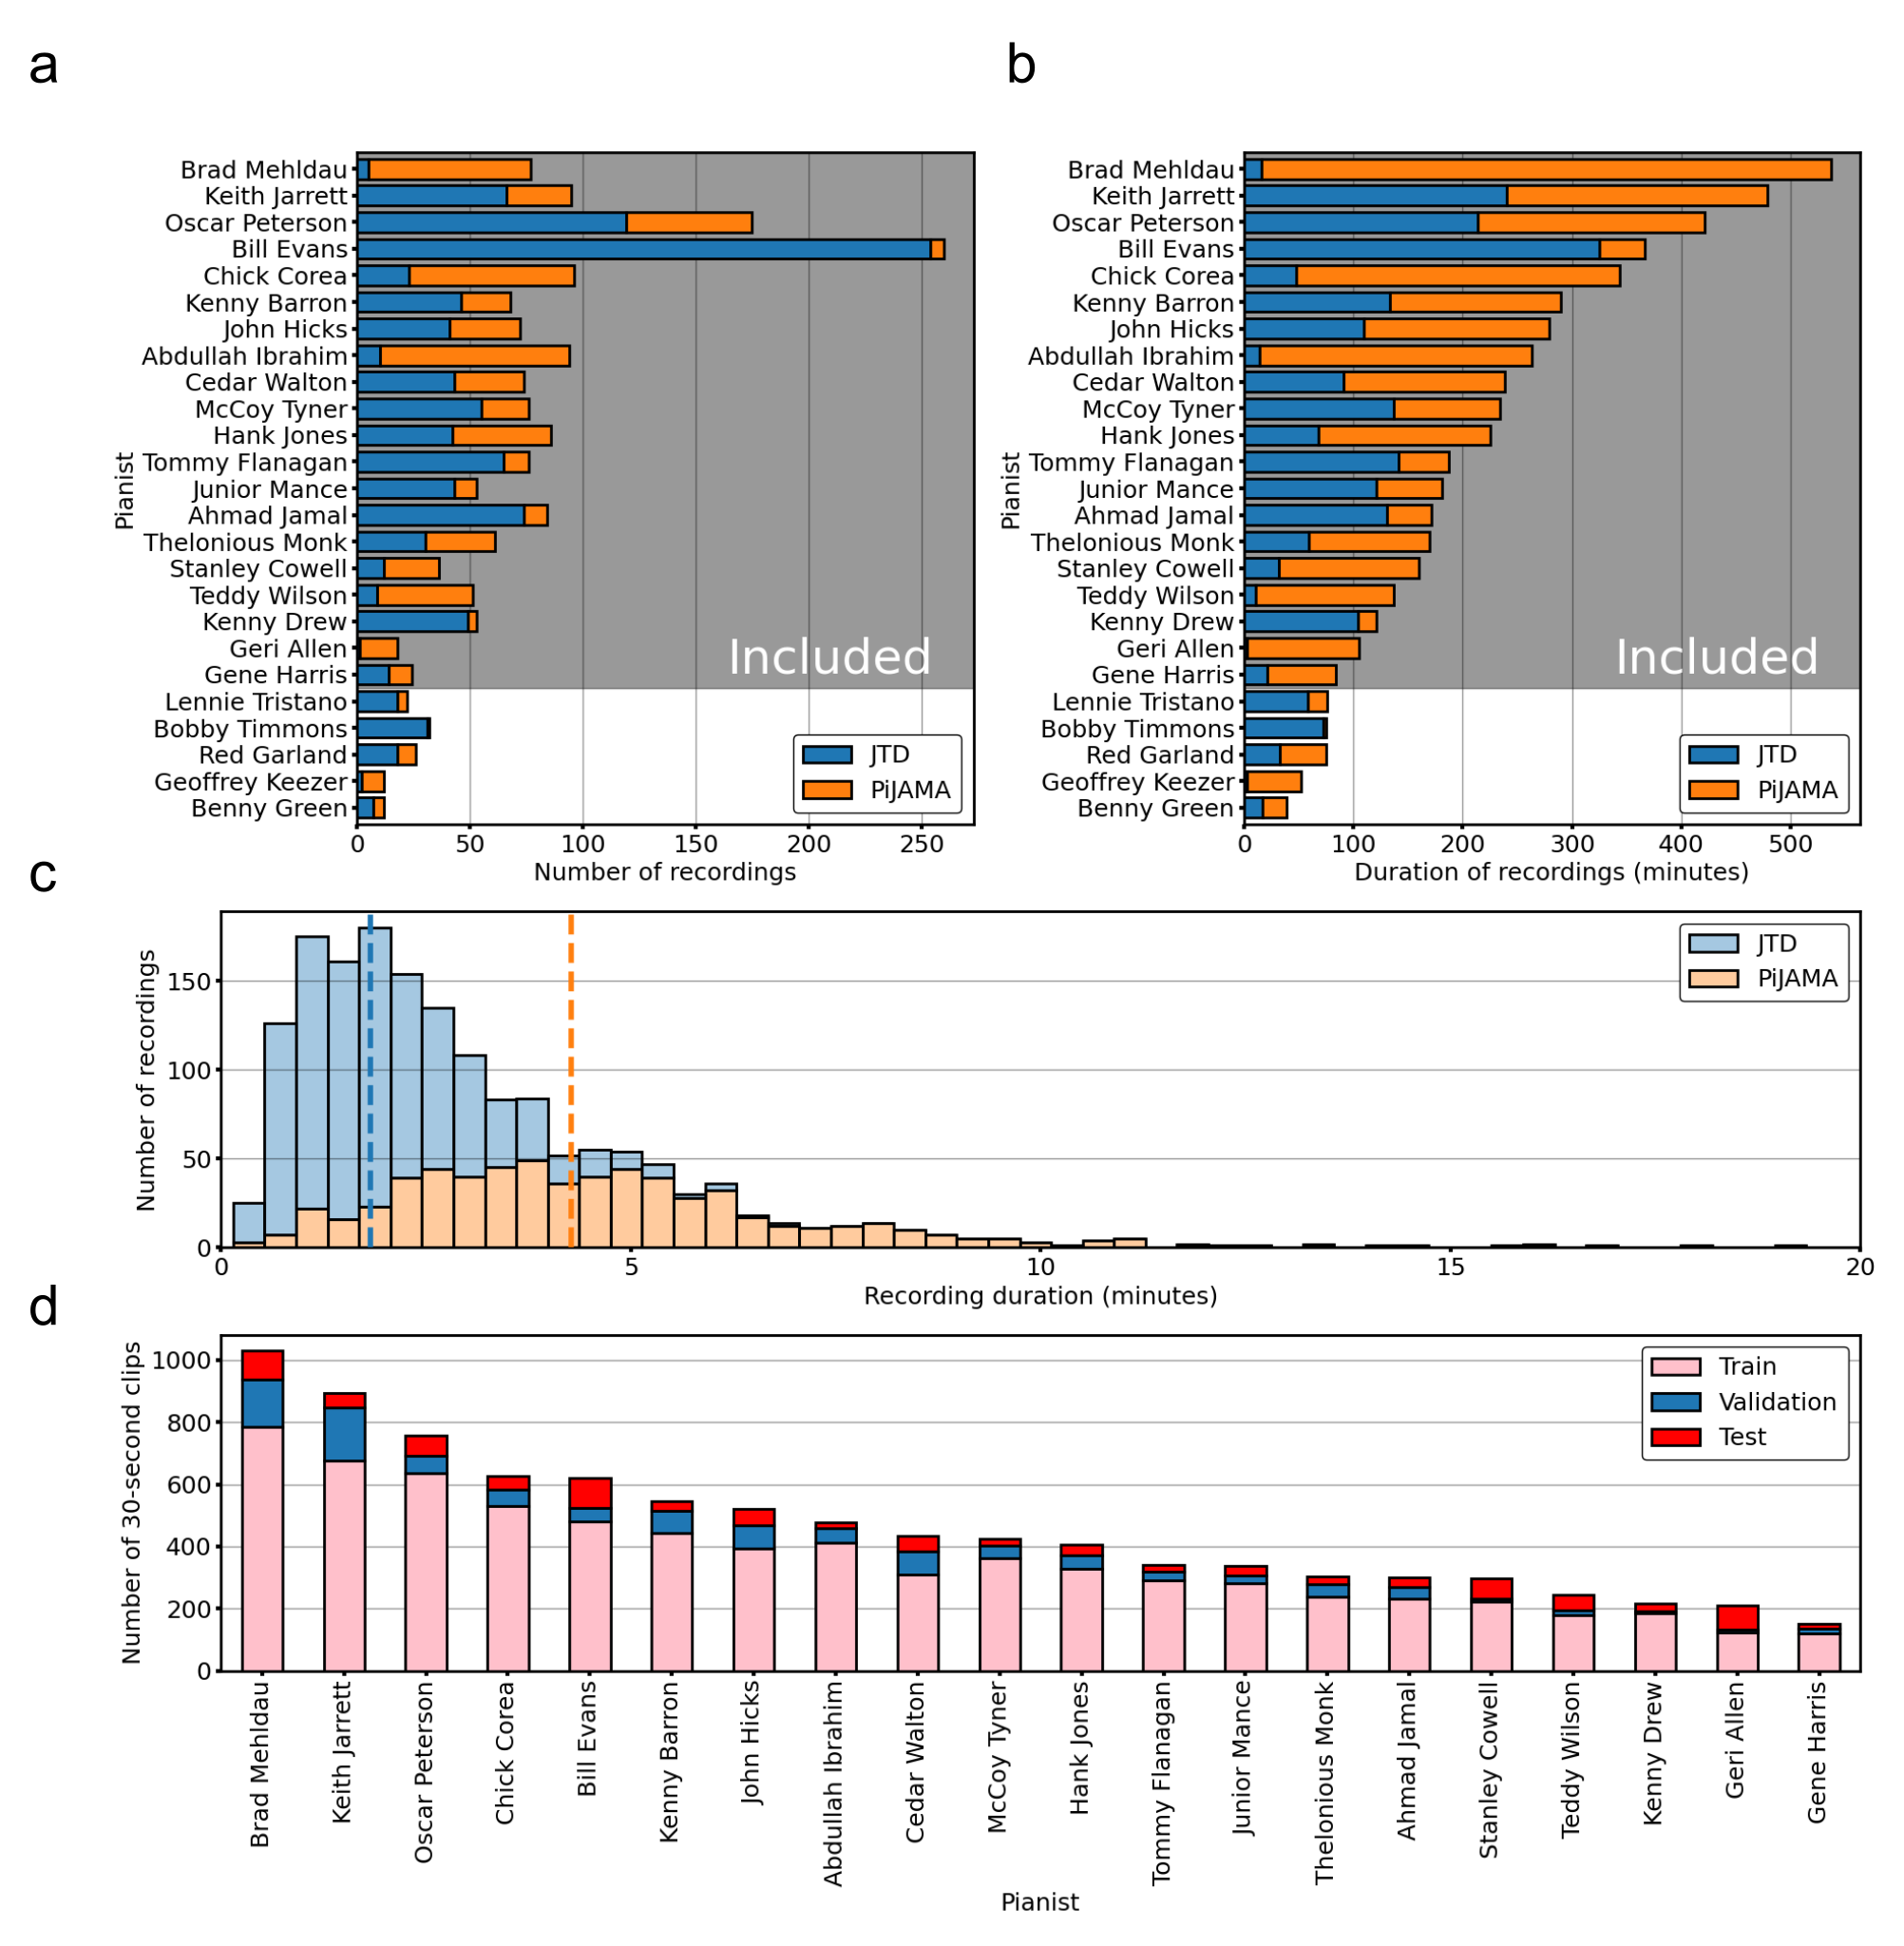
\includegraphics[width=1\textwidth]{figures/rsi_xai/figure_1.pdf}
  \caption[Dataset used for music performer identification.]{Dataset used for music performer identification. The upper row of panels show (a) the number of recordings by each pianist and (b) the total duration of their recordings, stratified by source database. Pianists are sorted in descending order by total duration, with the shaded area indicating when this is greater than 80 minutes. (c) shows the distribution of recording durations across tracks in both databases, with dashed lines representing the median recording duration. (d) shows the number of 30-second clips in each split of the dataset used to train the neural networks.}
\label{fig:rsi_dataset}
\end{figure}

Twenty-five different pianists have at least one recording in both datasets (Figure~\ref{fig:rsi_dataset}a). However, the cumulative duration of all recordings varies substantially between performers, from less than half an hour to over nine hours (Figure~\ref{fig:rsi_dataset}b). Consequently, we remove pianists with fewer than 80 minutes of recordings across \GLS{JTD} and \GLS{PiJAMA}. This leaves 1,629 performances by twenty pianists, with a total duration of 84 hours. Our dataset includes a greater number of recordings from \GLS{JTD} (1,001) than \GLS{PiJAMA} (628). However, the \GLS{PiJAMA} recordings (which are all full-length performances) are typically longer than those in \GLS{JTD} (which consist only of the piano solo in a recording), with a median duration of 4 minutes 18 seconds versus 1 minute 51 seconds (Figure~\ref{fig:rsi_dataset}c).

We randomly split these recordings into training, validation, and test subsets in the ratio $8:1:1$. These splits are stratified by source database, such that a proportional number of solo and ensemble performances are included in each subset. We use these splits to train and evaluate all of the models described in the remainder of the chapter. Note that we do not stratify our splits on either a \textit{composition}- or \textit{album}-level, which can minimise over-fitting when training classification models on music data \citep{Zhang2023-Symbolic, Rodriguez-algarra2019}. In the first case (and, unlike Western classical music), different performances of the same composition in jazz are usually very different, due to the emphasis on improvisation; in the second case, symbolic music representations such as MIDI ``piano rolls'' remove almost all acoustic information from a signal, which a model can otherwise learn to rely on \citep{Edwards2023}.

For the models described in Section~\ref{sec:rsi_handcrafted_features_approach}, features are extracted from an entire recording. For the neural networks in Sections~\ref{sec:rsi_representation_learning_approach} and~\ref{sec:rsi_factorised_inputs_approach}, we first segment each recording into 30-second clips (Figure~\ref{fig:rsi_dataset}d), with each clip inheriting the performer label of its parent recording during training. The hop size for each clip is 30 seconds during inference and varies between 15 and 30 seconds during training, as part of our data augmentation pipeline (described in Section~\ref{sec:rsi:data_augmentation}). During training, the classification loss is calculated using class probabilities estimated separately from each clip. During evaluation, we produce a track-level accuracy metric comparable with the models trained on entire recordings in Section~\ref{sec:rsi_handcrafted_features_approach} by averaging the class probabilities estimated across all clips taken from a single parent recording \citep[as in][]{Kong2020}. 

\section{Handcrafted Features Approach}\label{sec:rsi_handcrafted_features_approach}

\subsection{Methods}\label{sec:rsi_handcrafted_methods}

We train three classical supervised-learning architectures to identify the pianist playing in each recording using a hand-crafted set of features. These models are: random forests (\GLS{RF}, also used in Section~\ref{sec:rsos_methods}), support vector machines with linear kernel (\GLS{SVM}), and (regularised) multinomial logistic regression (\GLS{LR}). All three architectures have been widely used in previous computational work involving the modelling of musical style \citep{Alvarez2024, Deepaisarn2023, Eppler2014, Ramirez2010, Saunders2004, Widmer2004}. The implementations are taken from the \texttt{scikit-learn} (version \texttt{1.5.1}) Python library \citep{Pedregosa2011}.

\subsubsection{Feature Extraction}\label{sec:rsi_handcrafted_feature_extraction}

While these models could be trained on a wide variety of predictive features, we restrict ourselves to those reflecting the use of harmony and melody by performers, as these can be extracted simply from a musical transcription \citep[e.g.,]{Ens2020}. For an analogous approach studying rhythmic features obtained from many of the same recordings considered here, see Chapter~\ref{chap:rhythm_rsos}.

\begin{figure}[!ht]
  \centering
  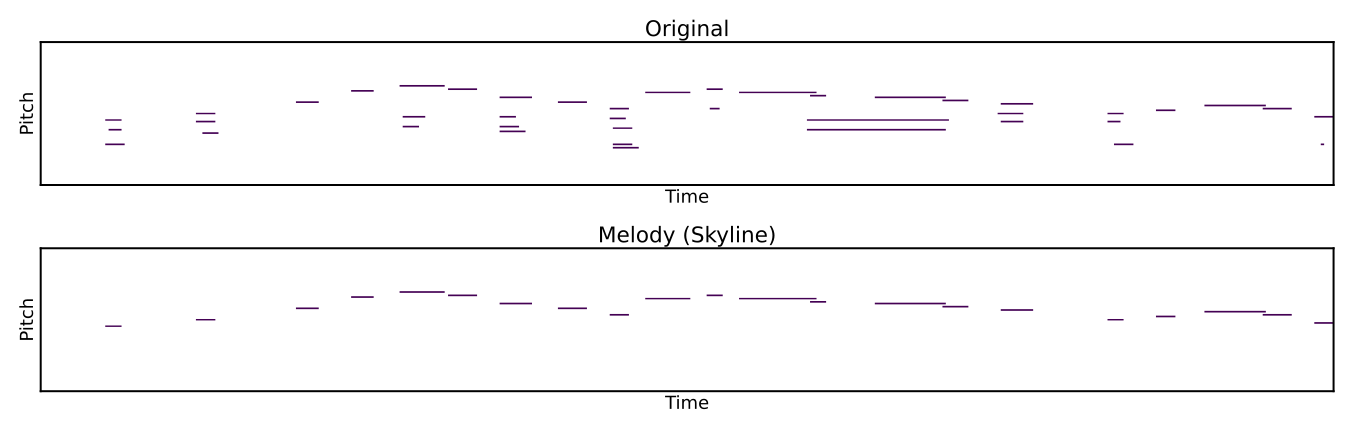
\includegraphics[width=1\textwidth]{figures/rsi_xai/figure_s1.pdf}
  \caption[Melody extraction results.]{Melody extraction results. The top panel shows ten seconds of a MIDI transcription and the bottom panel shows the same transcription after applying the implementation of the ``Skyline'' algorithm \citep{Uitdenbogerd1998} used in this work. When the same transcription was processed using the model described by \citet{Chou2024}, no notes were detected as being part of the melody.}
\label{fig:rsi_sm_melody_extraction_results}
\end{figure}

Extracting melody from a symbolic representation of a polyphonic musical performance is a challenging task. Ideally, we would use a sophisticated algorithm that either simulates underlying cognitive procedures involved in melody perception \citep[e.g.,][]{Sauve2018} or that learns to identify melodies from large annotated corpora of polyphonic music. Some deep learning architectures do exist that attempt the latter task \citep[e.g.,][]{Chou2024}, but we found that they performed badly on our data, with very few melody notes identified successfully and the majority of the output being empty (Figure~\ref{fig:rsi_sm_melody_extraction_results}). A possible explanation is that the data used to train these models often does not include jazz piano performances.

A simpler method is the ``skyline'' algorithm outlined by \citet{Uitdenbogerd1998}, which extracts the note with the highest pitch among the concurrent notes played at every unique onset time. This approach has drawbacks --- for instance, the extracted notes may ``leap'' between accompaniment and melody. However, in the absence of any more sophisticated methods developed for jazz piano, we nonetheless believe that it represents the best approach to this task. These drawbacks can also be controlled to a certain extent by developing heuristics that filter the ``melodies'' extracted from the skyline (see below).

Before applying the algorithm, we quantise a transcription by ``snapping'' note onsets to the nearest 100 ms (i.e,. 10 frames). This value is roughly equivalent to the duration of a triplet eighth note at the mean tempo of the recordings contained in both the full \GLS{JTD} and the smaller \GLS{JTD-300} subset (see Sections~\ref{sec:jtd_tempo} and~\ref{sec:rsos_tempo_features}, respectively). We then apply the skyline and obtain a vector of pitch classes, from which we extract $n$-grams (i.e., melodic ``chunks'' obtained over a sliding window). We remove $n$-grams that have either a total span of greater than 12 semitones or that have at least one duration greater than 2 seconds between successive offsets and onsets prior to quantisation. This first heuristic removes cases where the skyline conceivably ``leaps'' between melody and accompaniment, while the second removes cases where $n$-grams might be collected between the boundaries of a musical phrase. Finally, we convert each $n$-gram into a transposition-invariant representation by computing the difference between successive pitch classes.

\begin{figure}[!ht]
  \centering
  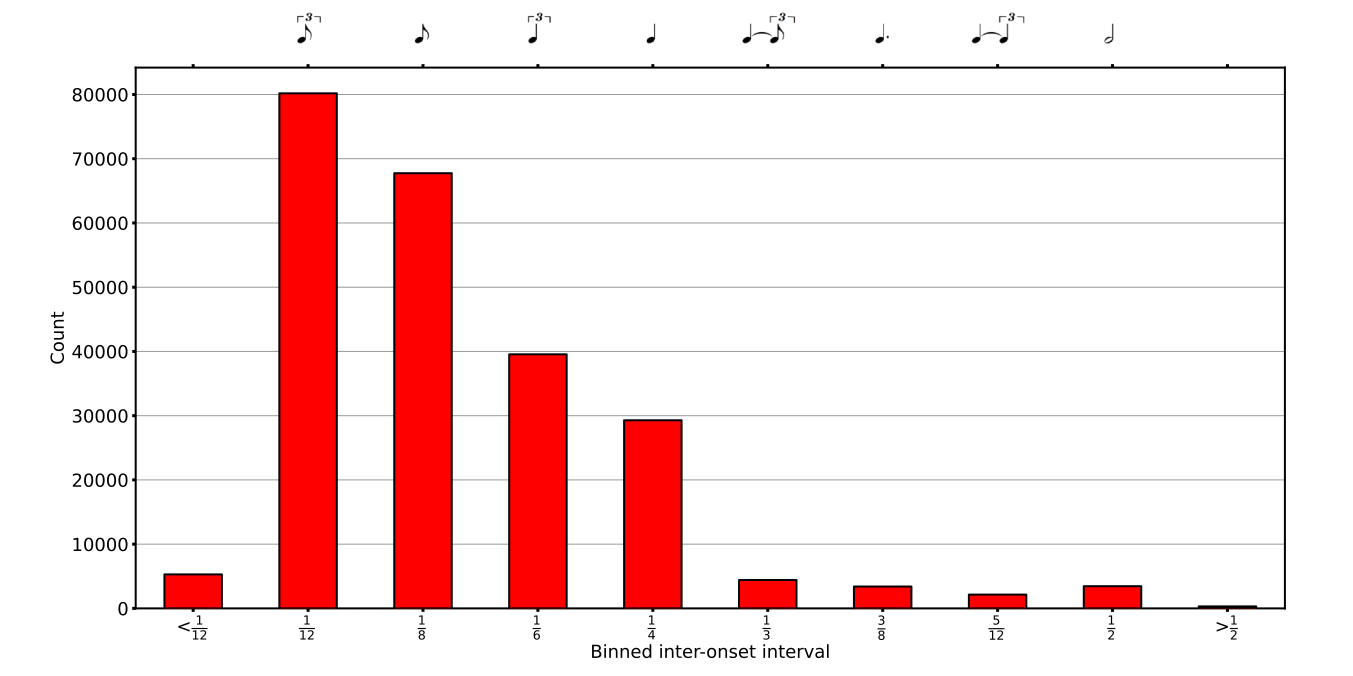
\includegraphics[width=1\textwidth]{figures/rsi_xai/figure_s2.pdf}
  \caption[\GLS{LR} accuracy with different values of $n$.]{\GLS{LR} accuracy with different values of $n$. The left panel shows changes in accuracy when the maximum value of $n$ used to extract melody and harmony features increases, from 3 to 8 inclusive. The right panel shows equivalent changes when the minimum value of $n$ increases. All accuracy scores are the results of optimising hyperparameters separately using random sampling for each value of $n$ (see Section~\ref{sec:rsi_handcrafted_training} in the full text) and are obtained for the validation split of the dataset.}
\label{fig:rsi_sm_lr_extraction_at_n}
\end{figure}

We use values of $n \in \{3, 4, 5, 6, 7\}$ when extracting melodic patterns from each transcription. In Figure~\ref{fig:rsi_sm_lr_extraction_at_n}, we demonstrate empirically that these values of $n$ are sufficient to achieve ceiling accuracy for the \GLS{LR} model when predicting the held-out validation split of the dataset, and that using larger values of either $\text{min}(n)$ or $\text{max}(n)$ does not increase performance \citep{Alvarez2024}. However, this does mean that some of our melodies obtained with lower values of $n$ can more accurately be described as short patterns, rather than full-length phrases. Nonetheless, we note that learning such melodic ``chunks'' does often form a key part of jazz pedagogy \citep{Berliner1994}. For an analogous procedure that solely considers longer melodic patterns in jazz, see \citet{Frieler2018}.

To extract harmony features from the MIDI transcription, we follow a method similar to \citet{Bantula2016}. First, we quantise the transcription to the nearest 100 ms according to the onset time of each note, as before. We keep quantised frames that contain $n \in \{3, 4, 5, 6, 7\}$ notes from each performance --- in other words, chord voicings that contain between three (i.e., triads) and seven notes. We discard chords with two or more leaps of greater than 15 semitones between two adjacent pitches in the chord, since such chords are more-or-less unplayable within an ordinary hand-span, and so are likely to correspond to transcription errors instead. Finally, we convert each chord into a transposition-invariant representation by expressing every pitch in terms of the number of semitones it lies above the lowest note in the chord. Note that we choose not to subtract the skylined melody as the highest note of every chord could theoretically have both a harmonic and melodic function, such as in the ``locked hands'' style of jazz piano performance \citep{Levine2011-1}.

We obtain counts for a total of 484,039 features (430,841 $n$-grams, 53,198 voicings) for the 1,629 recordings in the dataset. Similar to how text-based authorship models typically remove both frequent (i.e., ``stop'') and infrequent words \citep{Schonlau2017}, we then discard features contained in fewer than 10 and more than 1,000 recordings in order to reduce the size of the vocabulary. This leaves 21,670 features (17,918 melodic, 3,752 harmonic), with the reduced number of features explainable by a large number of melodic patterns and chord voicings that appear in very few recordings. We transform the matrix of feature counts to a normalised representation using the term frequency-inverse document frequency (\GLS{TF-IDF}) method, previously used for composer classification by \citet{Alvarez2024}. We found that \GLS{TF-IDF} substantially improved predictive accuracy compared with other techniques such as $z$-transformation.

\begin{figure}[!ht]
  \centering
  \includegraphics[width=1\textwidth]{figures/rsi_xai/figure_2.pdf}
  \caption[Feature counts for handcrafted models.]{Feature counts for handcrafted models. Each panel shows the counts of the twenty most frequently occurring (a) melody and (b) harmony features across all recordings and splits of the dataset. The $x$-axis values can be interpreted as the number of semitones from an initial starting note.}
\label{fig:rsi_feature_counts}
\end{figure}

We show counts for the twenty harmony and melody features that occur most frequently after filtering in Figure~\ref{fig:rsi_feature_counts}. Each feature can be interpreted as showing the number of semitones away from an initial starting pitch, such that the feature $(0, -1, -2, -3)$ becomes pitches $(\text{C}, \text{B}, \text{B}\flat, \text{A})$ or alternatively $(\text{G}, \text{G}\flat, \text{F}, \text{E})$. The melody features that occur most often are either alternations of ``perfect'' intervals, such as the octave $(0, -12, 0)$ and fifth $(0, -7, 0)$, or scalar fragments, such as a descending chromatic scale $(0, -1, -2, -3)$ or ascending minor scale $(0, 2, 3, 5)$ As might be expected, shorter patterns appear more frequently than longer ones, with the twenty most common features only containing three or four notes. Several of the harmony features that occur most frequently can be understood with relation to familiar chord types, such as major $(0, 4, 7)$ and minor $(0, 3, 7)$ triads in root position. Both the first $(0, 3, 8)$ and second $(0, 5, 9)$ inversion of the major triad are also common, as are ``stacked'' octave $(0, 12, 24)$ and perfect fourth $(0, 5, 10)$ intervals.

\subsubsection{Training}\label{sec:rsi_handcrafted_training}

\begin{table}[!ht]
    \centering
    \caption[Optimised parameters for \GLS{RF} performer identification model.]{Optimised parameters for \GLS{RF} performer identification model. These parameters resulted from the randomised search used to select parameters for the random forest classifier. Note that, when values for a parameter are sampled from either a uniform distribution $\mathcal{U}$ or logarithmic distribution $\mathcal{L}$ (with base 10), these are given in the range (start, stop).}
    \label{tab:rsi_sm_rf_optimised_parameters}
    \begin{tabular}{l c p{4cm} c}
        \toprule
        \textbf{Parameter} & \textbf{Values} & \textbf{Description} & \textbf{Result} \\
        \midrule
        \texttt{n\_estimators} & $\sim \mathcal{U}(10, 401)$ & Number of trees & 265 \\
        \texttt{max\_depth} & $\sim \mathcal{U}(1, 41)$ & Maximum depth of each tree & 26 \\
        \texttt{max\_features} & $\sim \mathcal{U}(0.0001, 1)$ & Proportion of features for best split & 0.148 \\
        \texttt{bootstrap} & \{True, False\} & Whether or not to use bootstrap samples & False \\
        \texttt{min\_samples\_leaf} & $\sim \mathcal{U}(1, 11)$ & Minimum samples per leaf & 3 \\
        \texttt{min\_samples\_split} & $\sim \mathcal{U}(2, 11)$ & Minimum samples to split a node & 7 \\
        \bottomrule
    \end{tabular}
\end{table}

\begin{table}[!ht]
    \centering
    \caption[Optimised parameters for \GLS{SVM} performer identification model.]{Optimised parameters for \GLS{SVM} performer identification model.}
    \label{tab:rsi_sm_svm_optimised_parameters}
    \begin{tabular}{l c p{4cm} c}
        \toprule
        \textbf{Parameter} & \textbf{Values} & \textbf{Description} & \textbf{Result} \\
        \midrule
        \texttt{C} & $\sim \mathcal{L}(0.001, 1000)$ & Regularisation parameter: smaller values imply stronger regularisation & 1.359 \\
        \texttt{class\_weight} & \{None, balanced\} & If balanced, adjusts weights inversely proportional to class frequencies & None \\
        \bottomrule
    \end{tabular}
\end{table}

\begin{table}[!ht]
    \centering
    \caption[Optimised parameters for \GLS{LR} performer identification model.]{Optimised parameters for \GLS{LR} performer identification model.}
    \label{tab:rsi_sm_lr_optimised_parameters}
    \begin{tabular}{l c p{4cm} c}
        \toprule
        \textbf{Parameter} & \textbf{Values} & \textbf{Description} & \textbf{Result} \\
        \midrule
        \texttt{C} & $\sim \mathcal{L}(0.001, 1000)$ & Identical to SVM & 37.017 \\
        \texttt{class\_weight} & \{None, balanced\} & Identical to SVM & balanced \\
        \texttt{penalty} & \{None, $\text{L}_2$\} & Penalty term to use & $\text{L}_2$ \\
        \bottomrule
    \end{tabular}
\end{table}

The process used to train each of the three models is the same. We generate a two-dimensional hyperparameter space (Tables~\ref{tab:rsi_sm_rf_optimised_parameters},~\ref{tab:rsi_sm_svm_optimised_parameters},~\ref{tab:rsi_sm_lr_optimised_parameters}), randomly sample possible configurations of parameters from this space (with $N = 1,000$ iterations), fit the model to the training split of the dataset, and measure the accuracy when predicting class labels for the validation split. We find that this many iterations is sufficient to achieve ceiling accuracy on the held-out validation data across all classifier types. We then use the hyperparameter configuration that resulted in the highest validation accuracy to predict the class labels of the held-out test split, and report the accuracy for this subset of the data as the overall performance of the model. For consistency with the neural networks we introduce later, we do not retrain the model on the training and validation splits after selecting the optimal hyperparameter configuration. A single iteration takes approximately 20 seconds for the \GLS{LR} model, 211 seconds for the \GLS{RF}, and 31 seconds for the \GLS{SVM}. All iterations run in parallel on a machine with 76 CPU cores.

\subsection{Results}\label{sec:rsi_handcrafted_results}

\subsubsection{Who is the Performer of an Unknown Musical Piece?}\label{sec:rsi_handcrafted_evaluation}

\begin{table}[!ht]
    \centering
    \caption[Results for models trained using handcrafted features on held-out test data.]{Results for models trained using handcrafted features on held-out test data. Note that scores for the \GLS{SVM} at higher than top-1 accuracy cannot be provided due to limitations in the \texttt{scikit-learn} implementation of this model.}
    \label{tab:rsi_sm_handcrafted_results}
    \begin{tabular}{l c c c c}
        \toprule
        \textbf{Architecture} & \multicolumn{4}{c}{\textbf{Accuracy (track)} $\uparrow$} \\ \cmidrule{2-5}
         & \textbf{Top-1} & \textbf{Top-2} & \textbf{Top-3} & \textbf{Top-5} \\ \midrule
        Random Forest (\GLS{RF}) & 0.454 & 0.626 & 0.706 & 0.785 \\
        Support Vector Machine (\GLS{SVM}) & 0.687 & -- & -- & -- \\
        Logistic Regression (\GLS{LR}) & \textbf{0.767} & \textbf{0.859} & \textbf{0.896} & \textbf{0.939} \\
        \bottomrule
    \end{tabular}
\end{table}

We show the accuracy of the three models in predicting the held-out test data in Table~\ref{tab:rsi_sm_handcrafted_results}. The \GLS{LR} model (with L2 or ``ridge'' regularisation as the penalty term) performs the best, achieving 0.767 top-1 accuracy when predicting the identity of the twenty jazz pianists considered here. The top-5 accuracy for this model is 0.939 --- meaning that, for nearly 95\% of unseen recordings, the actual pianist is within the five classes with the highest predictive probability estimated by this model, despite it only using melodic n-grams and chord voicings as input features. The \GLS{RF} and \GLS{SVM} models both perform worse, achieving 0.454 and 0.687 top-1 accuracy on the held-out test data, respectively.

\subsubsection{Which Domains are Important for Musical Style?}\label{sec:rsi_feature_importance_by_domain}

\begin{figure}[!ht]
  \centering
  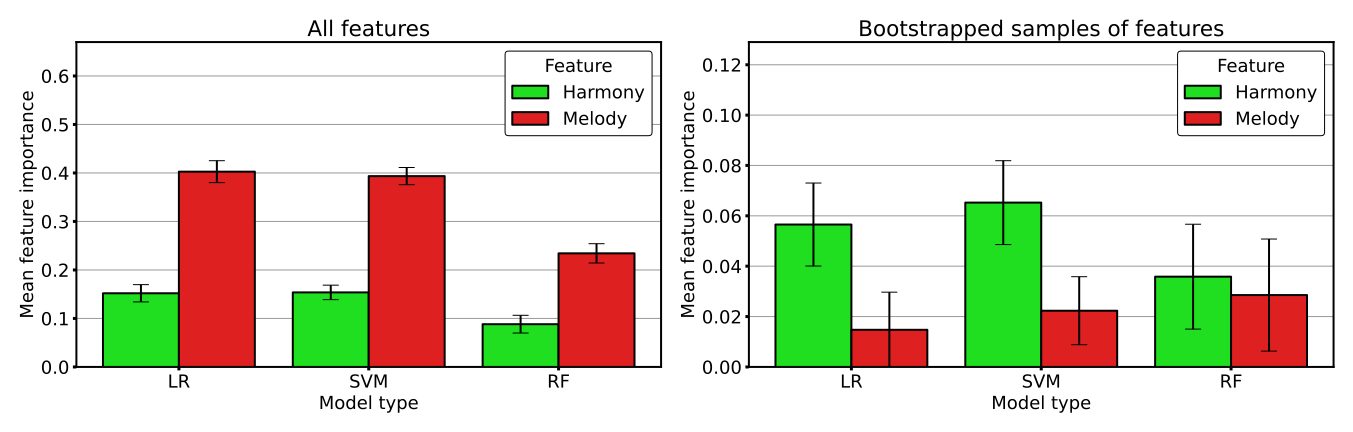
\includegraphics[width=1\textwidth]{figures/rsi_xai/figure_s3.pdf}
  \caption[Feature importance by domain and model type.]{Feature importance by domain and model type. Each bar shows the loss in test accuracy from permuting all melody or harmony features (left panel) and bootstrapped subsamples of 2,000 features (right panel), stratified by model type. Error bars show standard deviations ($N = 1,000$ iterations).}
\label{fig:rsi_sm_feature_importance_by_handcrafted_model_type}
\end{figure}

One way of ascertaining the relative importance of the input features used by these models is to calculate the decrease in predictive accuracy when the values obtained for a feature (or group of features) are permuted \citep{Breiman2001}. We compute feature importance by permuting either all harmony or all melody features and measuring the loss in held-out test accuracy for the \GLS{LR} versus predicting with the complete feature set. The accuracy loss (averaged over $N = 1,000$ iterations) when permuting $n$-grams is substantially greater than permuting chord voicings (0.403 vs. 0.152). Similar trends are observed for both the optimised \GLS{RF} and \GLS{SVM} models (Figure~\ref{fig:rsi_sm_feature_importance_by_handcrafted_model_type}). This might suggest that melodic patterns are more important than chord voicings in differentiating one jazz pianist from another. 

Given the imbalance in the number of features (with over twice as many $n$-grams than voicings), an alternative way to consider the importance of a single feature is to permute random subsets of $K$ melody or harmony features (sampled without replacement from the full feature space) and measure the mean loss in accuracy. With $K = 2,000$ features (approximately 10\% of the total number), the loss in accuracy for the \GLS{LR} is larger when permuting harmony than melody features (0.015 vs. 0.057: mean across $N = 1,000$ iterations). Similar trends are observable for all other model types (Figure~\ref{fig:rsi_sm_feature_importance_by_handcrafted_model_type}). This would suggest that the typical chord voicing has over three times the explanatory power of the typical melody $n$-gram; however, as the vocabulary of $n$-grams is much larger than the vocabulary of voicings, permuting all of these features leads to a proportionally greater drop in accuracy. 

\subsubsection{How Does Style Differ Between Performance Contexts?}\label{sec:rsi_feature_importance_by_dataset}

Another question we can ask is whether there are differences in improvisation style between solo and ensemble performances. To do so, we first fit the \GLS{LR} model to the entire dataset. We compute the absolute magnitude of each feature weight for each performer, take the maximum across performers, rank these in decreasing order, and then take the top-$k$ features (with $k = 2,000$, as before). These features correspond to the maximally predictive features across all performers. 

In other words, given a matrix of feature weights $W \in \mathbb{R}^{I \times J}$ extracted from the \GLS{LR} model, where $I$ is the number of performers (with $I = 20$) and $J$ is the number of features (with $J = 17,918$ for melody, $J = 3,752$ for harmony), we transform this into the matrix $W' \in \mathbb{R}^{I \times K}$ by first taking the maximum absolute value of each feature $j \in \{1, \dots, J\}$ across all performers $i \in \{1, \dots, I\}$ and then taking the top-$K$ of sorted values of $j$, such that
\begin{align}
W'_{i, k} = \text{sort} \left( \max_{i \in \{1, \dots, I\}} \left( |W_{i, j}| \right), \; \forall j \in \{1, \dots, J\} \right)_{i, k}, \ k \in \{1, \dots, K\}.
\end{align}

We then fit separate models to recordings from both datasets using only these features, extract the vector of $k$ weights for every performer, and calculate the correlation coefficients between equivalent vectors from both datasets. We also repeat this process for the top-$K$ harmonic features. Note that, while it would be possible to use all features here, many of these would likely be noise given the high dimensionality of the feature space, which could artificially deflate the correlations.

\begin{figure}[!ht]
  \centering
  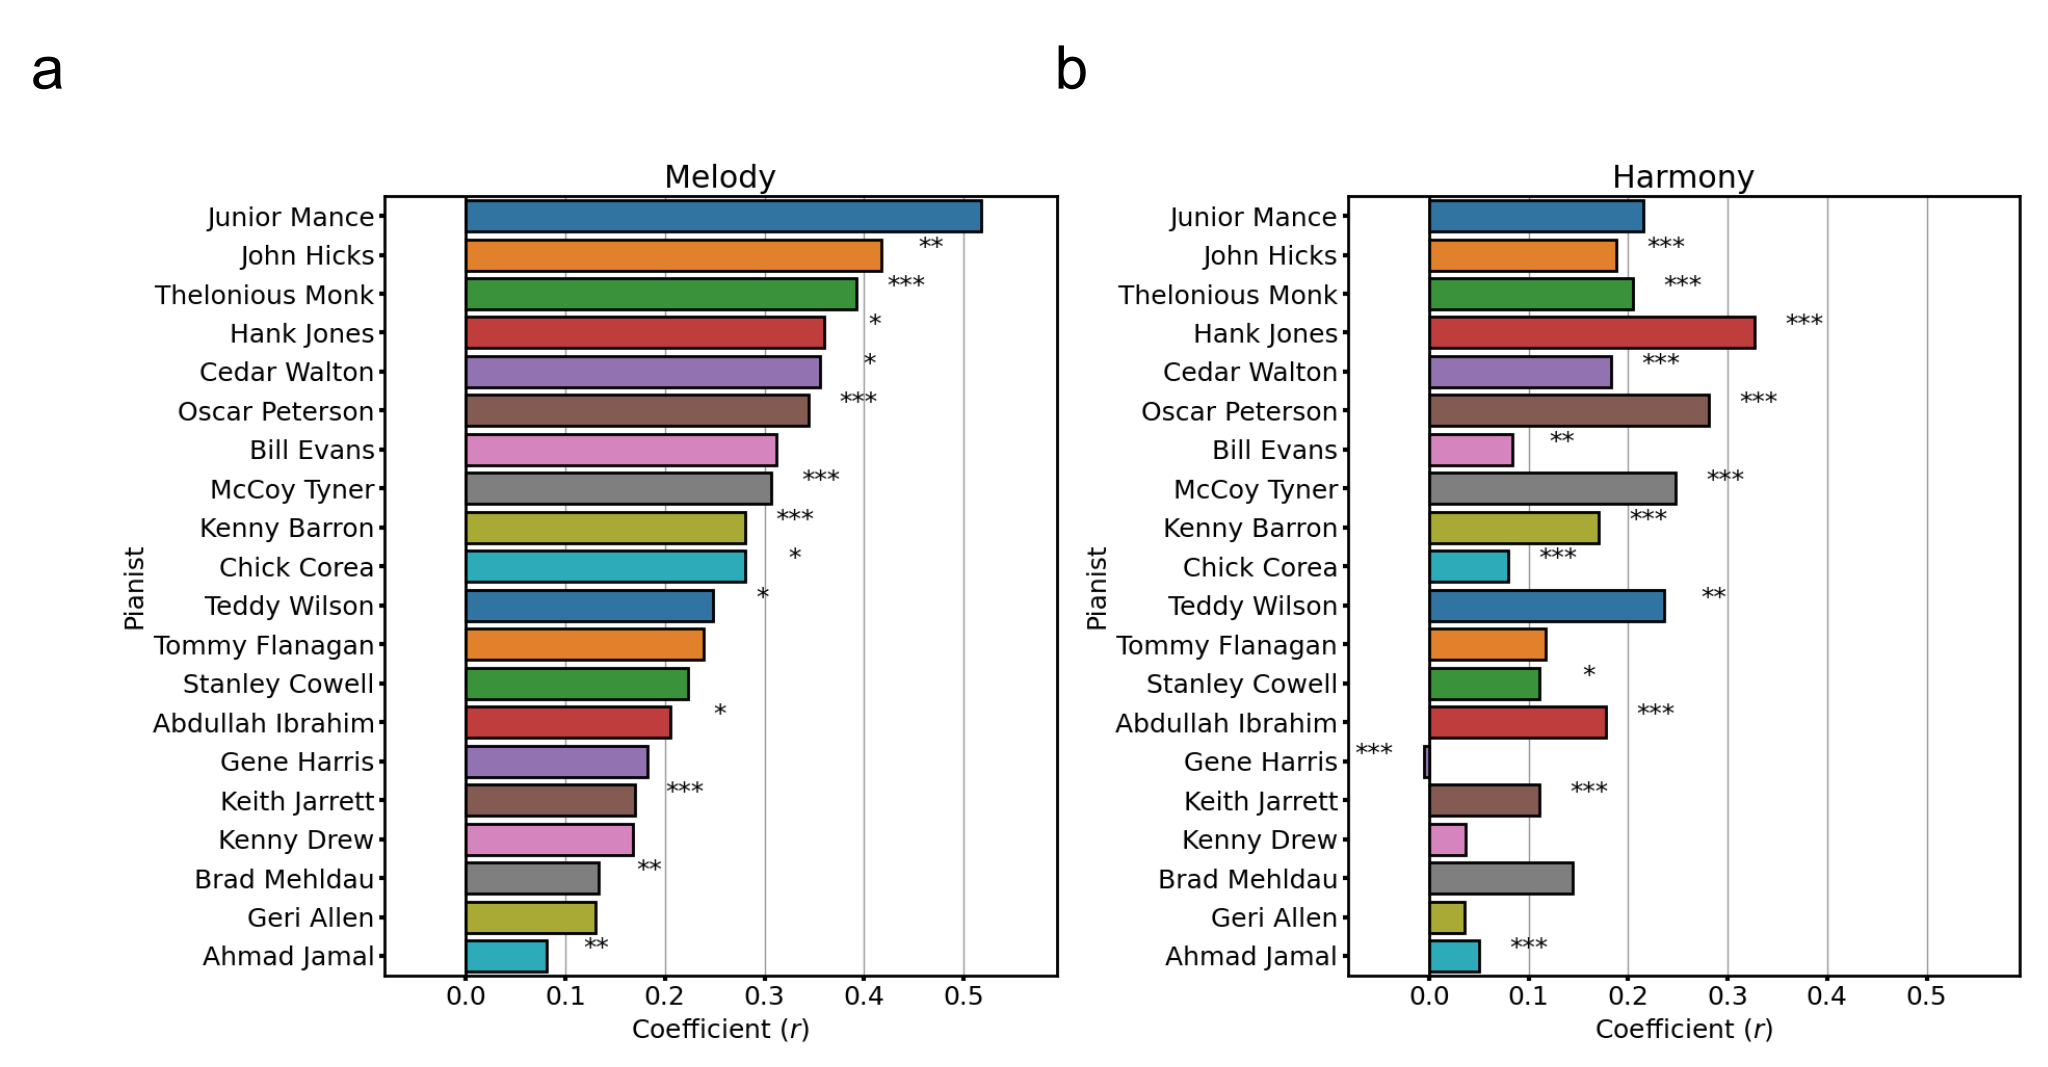
\includegraphics[width=1\textwidth]{figures/rsi_xai/figure_3.pdf}
  \caption[Relationships between databases.]{Relationships between databases. Each panel shows correlation coefficients obtained between the weights of every performer for models fitted using (a) melody and (b) harmony features. Performers are sorted in descending order of magnitude according to the correlations in panel (a). Asterisks show the significance of the observed coefficients ($^* \ p < .05, \ ^{**} \ p < .01, \ ^{***} \ p < .001$, with Bonferroni correction applied), calculated using permutation testing ($N = 1,000$ iterations).}
\label{fig:rsi_dataset_correlations}
\end{figure}

In nearly every case, these correlations are positive (melody: $\text{mean}(r) = 0.267$, $SD = 0.108$, harmony: $\text{mean}(r) = 0.150$, $SD = 0.087$: see Figure~\ref{fig:rsi_dataset_correlations}). To the extent that performer style differs between solo and ensemble performances, we would expect correlations to be lower across the datasets (i.e. between solo versus ensemble datasets) than within datasets. To test this hypothesis, we conduct a one-sided (left-tailed) permutation-based significance test, which involves randomly shuffling the dataset label for every recording prior to fitting the model, thereby obtaining a Monte Carlo null distribution of correlation coefficients ($N = 1,000$ iterations) against which we test our observed correlations. We apply Bonferroni correction for the number of feature sets (i.e., 2), thereby controlling false discovery rate on the performer level. These tests indicate that, in the majority of cases, the correlation between feature weights obtained from either dataset are significantly smaller than would be expected were the two datasets to be equivalent. 

This finding is broadly consistent with the literature on jazz improvisation, where musicians frequently comment on differences between playing unaccompanied versus with a group. For pianist John Lewis ``there is very little leeway in transferring your ideas from a group situation to a solo performance. You have a lot more freedom [when playing unaccompanied], but you have to learn how to discipline that freedom'' \citep[p. 81]{Lyons1983}. More specifically, Oscar Peterson noted how playing unaccompanied allowed him to use ``certain harmonic movements ... which [he] couldn't do with the trio'' \citep[p. 141]{Lyons1983}. A note can be made for Junior Mance, who demonstrated the greatest positive correlation between melody feature weights from both datasets ($r = 0.517$, $p = .218$): jazz critic Brian Priestley \citep[p. 319]{Carr1988} describes how ``his trio and solo routines are sometimes predictable ... highly rhythmic, bluesy''.

\subsubsection{Which Features are Associated With Particular Performers?}\label{sec:rsi_feature_importance_by_performer}

While this analysis is interesting in terms of demonstrating the importance of high-level musical dimensions (i.e., melody, harmony) towards improvisation style, it does not tell us which features influenced the model to classify individual performers --- in other words, which melodic patterns or chord voicings best define the style of one particular performer. \citet{Frieler2018} explored this task by ranking how frequently different jazz improvisers used particular melodic patterns. A related method was developed by \citet{Conklin2010}, who defined the distinctiveness of a pattern within a musical corpus as the degree to which it is over-represented with respect to an anti-corpus. 

We take a different approach by instead formalising the ``distinctiveness'' of a given musical feature for a particular performer using the weights it is associated with by our model. This helps mitigate the influence of features that are commonly used by all performers in the dataset (as a result of our \GLS{TF-IDF} pre-processing), while also avoiding the need to explicitly define an anti-corpus.

\begin{figure}[!ht]
  \centering
  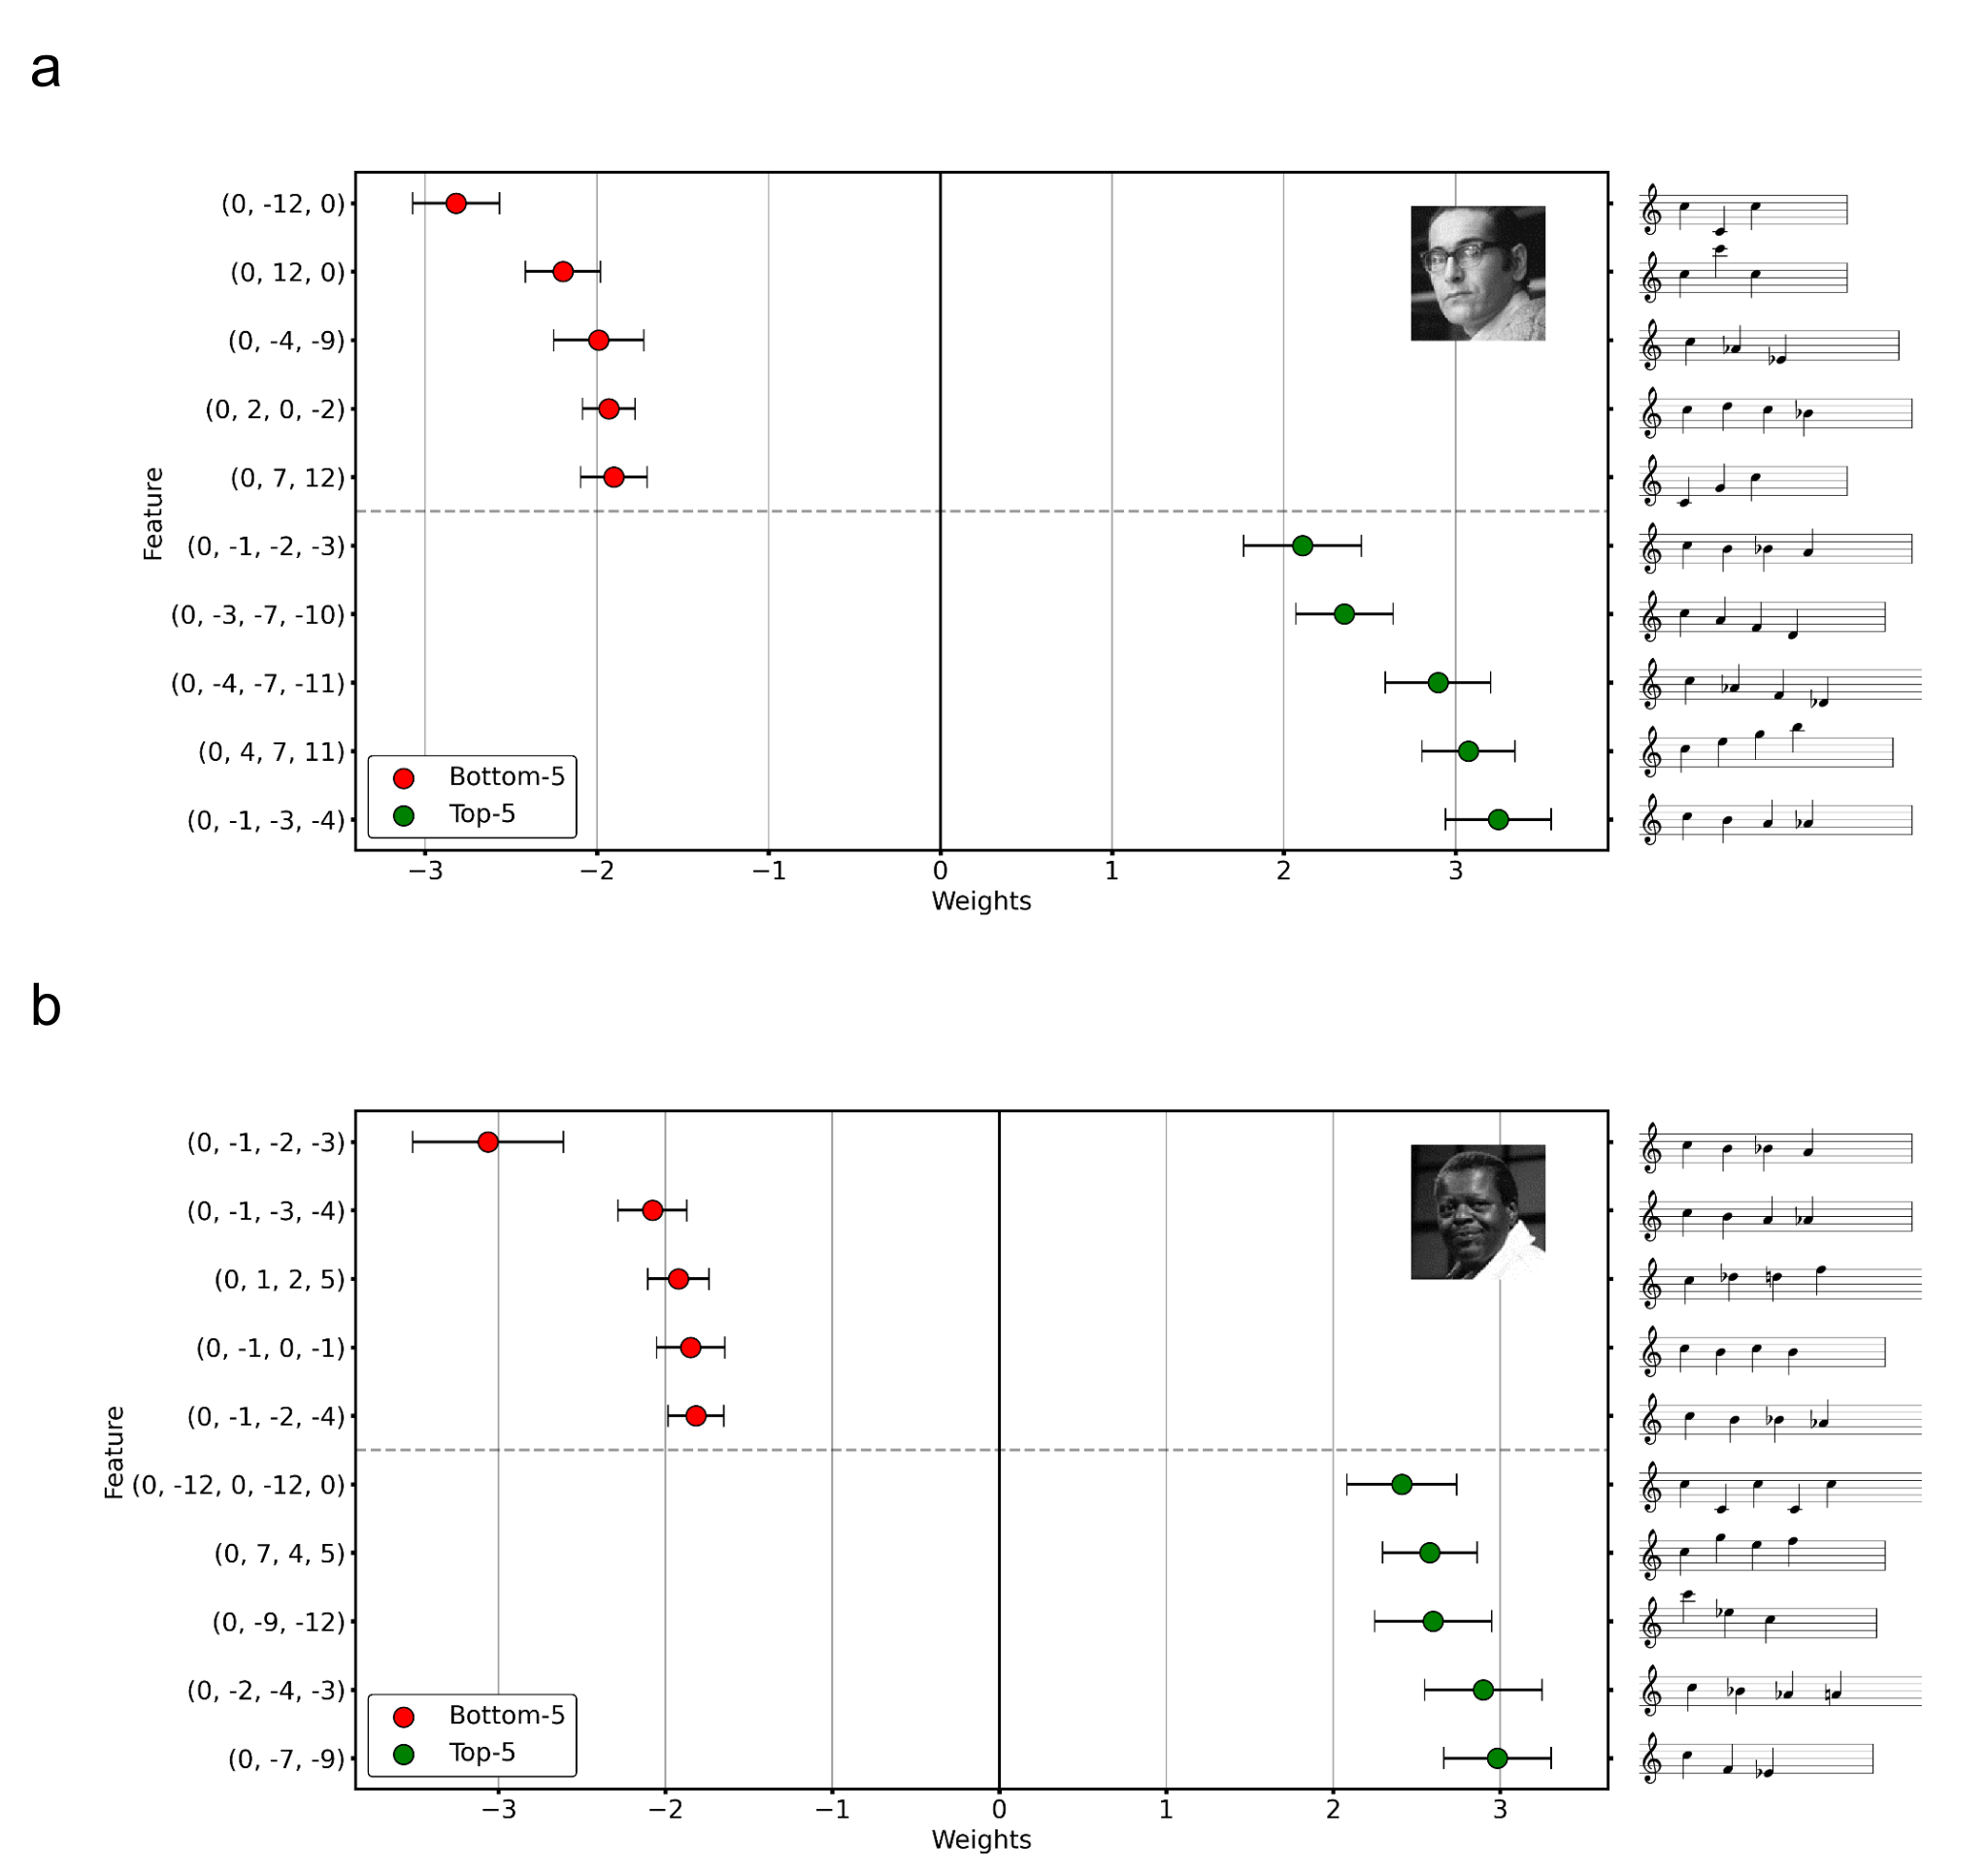
\includegraphics[width=1\textwidth]{figures/rsi_xai/figure_4.pdf}
  \caption[Most predictive melody features.]{Most predictive melody features. Both panels show feature weights obtained for the top and bottom five melody $n$-grams associated with classifications of (a) Bill Evans and (b) Oscar Peterson. Error bars show $SD$, calculated by bootstrapping the dataset used to fit the model ($N = 1,000$ iterations). Corresponding musical notation for every $n$-gram is on the right, transposed such that the first note is C and the mean pitch height is approximately centred around $G_4$. The pitch spelling for each feature is estimated using the algorithm described by \citet{Meredith2006}}
\label{fig:rsi_predictive_melody_features}
\end{figure}

We fit the \GLS{LR} model to the entire dataset and extract the weights obtained for each class and melody feature. Here, a positive weight indicates that the presence of the feature increases the likelihood of predicting a given class, while a negative weight decreases the likelihood. In Figure~\ref{fig:rsi_predictive_melody_features}, we show weights for the top and bottom five melody features associated with classifications of Bill Evans and Oscar Peterson --- the two pianists with the greatest number of individual recordings in the dataset (Figure~\ref{fig:rsi_dataset}a). We provide similar graphs for all other pianists as part of Appendix~\ref{chap:rsi_appendix_weights} (Figures~\ref{fig:rsi_sm_ibrahim_melody}--\ref{fig:rsi_sm_flanagan_melody}). The five most distinctive melody features for each pianist can also be listened to within the context of their performances as part of an interactive web application we have developed (see Footnote~\ref{note:rsi_webapp}, subheading ``melody'').

For Bill Evans, two of the five patterns with the strongest weighting outline either a descending major $(0, -4, -7, -11)$ or minor $(0, -3, -7, -10)$ seventh arpeggio, beginning on the seventh and falling to the root. Both patterns appear frequently in jazz pianist Jacky Naylor's pedagogical textbook outlining Evans' improvisation style \citep{Naylor2024-BE}. The descending major seventh arpeggio, for instance, is used by Evans to outline a harmonic progression (with the top note descending stepwise through a scale: ``lick 50''), to decorate an extended chord (with the second note of the pattern becoming the top note of the next repetition: ``lick 65''), and over the minor chord in a ``turnaround'' harmonic progression (with the seventh functioning as the ninth above the bass: ``lick 23''). 

Several of the patterns with the strongest weighting for Oscar Peterson can be considered melodic ``enclosures''. For example, the pattern $(0, -2, -4, -3)$ is described by \citet{Naylor2024-OP} in his textbook on Peterson's style as a ``chromatic enclosure around the third'' (``lick 82''), approaching the major third of the underlying harmony from above and then below. Likewise, the $(0, 7, 4, 5)$ pattern acts as a ``scale note enclosure'' (``lick 23''), approaching the note a perfect fourth above the starting pitch diatonically from above and then below. 

We can make observations for several of the other performers shown in Appendix~\ref{chap:rsi_appendix_weights}. McCoy Tyner (Figure~\ref{fig:rsi_sm_tyner_melody}) is associated with multiple features that outline a perfect fourth interval ($\pm5$), including $(0, -5, -7, 0, -5)$ and $(0, 5, 3, 0)$: Tyner himself has acknowledged that the use of this interval is ``one of the characteristics of [his] style'' \citep[p. 97]{Sidran1992}. Thelonious Monk (Figure~\ref{fig:rsi_sm_monk_melody}) is associated with a descending whole-tone pattern $(0, -2, -4, -6, -8)$ that theorist Gunther \citet[p. 231]{Schuller1965} claimed Monk was ``addicted'' to. Finally, Tommy Flanagan (Figure~\ref{fig:rsi_sm_flanagan_melody}), perhaps best known for accompanying saxophonist John Coltrane on his album ``Giant Steps'', is strongly associated with a $(0, 2, 4, 7)$ scalar pattern that Coltrane used throughout this record \citep[discussed also in][]{Frieler2018}.

Appendix~\ref{chap:rsi_appendix_weights} (Figures~\ref{fig:rsi_sm_ibrahim_harmony}--\ref{fig:rsi_sm_flanagan_harmony}) contains analogous figures for the harmony features. While we reserve a full analysis for subsequent work, several observations can nonetheless be made here. For instance, Bill Evans (Figure~\ref{fig:rsi_sm_evans_harmony}) is strongly associated with the cluster $(0, 1, 5)$, which can be considered a minor voicing containing the ninth, minor third, and fifth; it was in the use of such ``rootless'' voicings that Evans was particularly known for \citep{Levine2011-1}. Many other features can be considered elaborations of an underlying dominant harmony, such as the $(0, 16, 22, 27)$ voicing associated with Cedar Walton (Figure~\ref{fig:rsi_sm_walton_melody}) --- commonly known to rock musicians as the ``Jimi Hendrix chord'' \citep{Shapiro1995}. Finally, McCoy Tyner (Figure~\ref{fig:rsi_sm_tyner_harmony}) is again associated with voicings built on the fourth interval, including $(0, 5, 10)$ and $(0, 6, 11)$.

\begin{figure}[!ht]
  \centering
  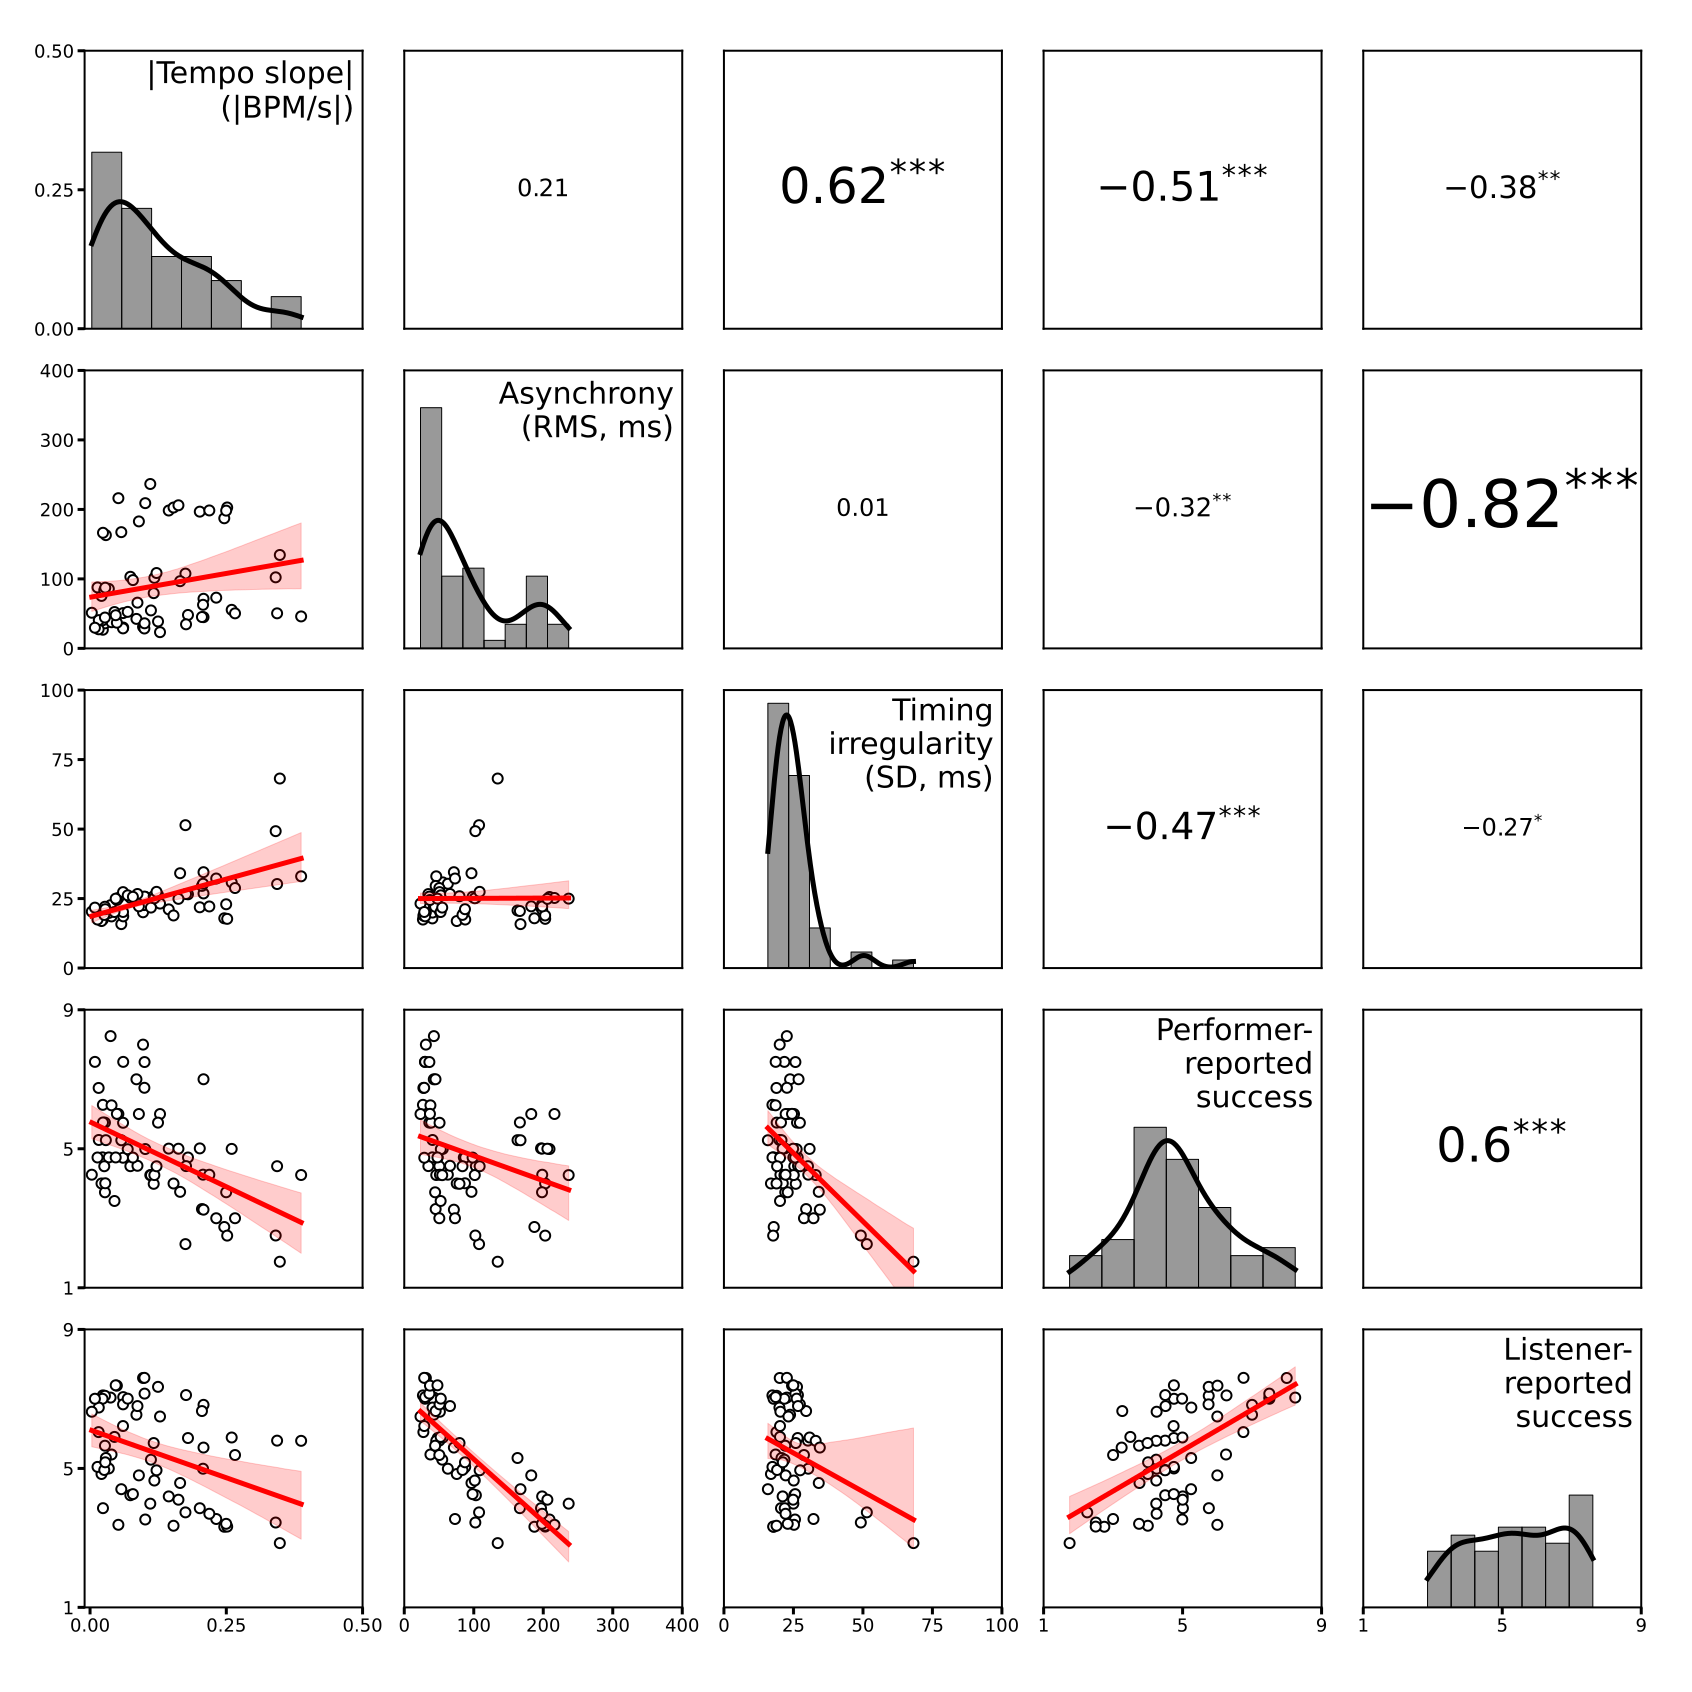
\includegraphics[width=1\textwidth]{figures/rsi_xai/figure_5.pdf}
  \caption[Feature counts decomposed with \GLS{PCA}.]{Feature counts decomposed with \GLS{PCA}. The horizontal and vertical axes respectively show melody feature and performer projections onto (a) principal components 1 and 2 and (b) components 3 and 4. Values are linearly scaled separately for each dimension to within the range $(-1, 1)$. Each melody feature shows the number of semitones relative to the initial note $0$, as in Figure~\ref{fig:rsi_feature_counts}. To select the melody features to plot, we divide the two-dimensional representation into eight circular ``slices'' and within each slice plot the 5 features with the highest absolute magnitudes. Performers are shown by their initials, such that \texttt{BE} corresponds to Bill Evans.}
\label{fig:rsi_pca_feature_counts}
\end{figure}

\subsubsection{How are the Styles of Particular Performers Related?}

These preceding analyses focussed on individual $n$-grams, but it is also possible to use dimensionality reduction to visualise larger-scale clusters of $n$-gram usage in order to relate the melodic styles of every performer in our dataset. Here we use principal component analysis (\GLS{PCA}); we apply it to melodic $n$-grams of length 4, of which there are 5,838. We process the raw feature counts with \GLS{TF-IDF} as before (see Section~\ref{sec:rsi_handcrafted_feature_extraction}), then centre them on their means with $z$-transformation and scale the results between the range $(0, 1)$ according to the minimum and maximum values of every feature. We apply \GLS{PCA} to the result to obtain a set of principal components and then project each performer onto the same space by taking the dot product of their averaged feature counts with every component. In Figure~\ref{fig:rsi_pca_feature_counts}, we plot all performer classes and a subset of the features that load most strongly onto the first four principal components. 

Features that load positively onto principal component 1 typically consist of small scalar patterns with a span of less than a perfect fifth, such as $(0, -2, -4, -5)$, $(0, 2, 3, 5)$, and $(0, -2, -3, -7)$ \citep[the inverted, minor version of the``Coltrane pattern'': see Section~\ref{sec:rsi_feature_importance_by_performer} and][]{Frieler2018}. Keith Jarrett, Tommy Flanagan, and Kenny Barron all load positively onto this component: Figure~\ref{fig:rsi_sm_flanagan_melody} shows how Flanagan uses several of these melodic patterns. Features that load negatively onto component 1 span a much larger distance, such as $(0, -1, -2, 8)$ and $(0, 1, 6, -1)$, with Abdullah Ibrahim, Ahmad Jamal, and Thelonious Monk also loading negatively here.

Features that load positively onto component 2 involve chromatic patterns, such as $(0, -1, -2, -3)$ and $(0, -1, -3, -2)$, with Bill Evans loading positively onto this component. Features that load negatively consist of the same interval played multiple times in either an ``up-down-up'' or ``down-up-down'' fashion, including $(0, -7, 0, -7)$ and $(0, 5, 0, 5)$, while Brad Mehldau, Junior Mance, and McCoy Tyner all load negatively onto component 2 also. Here, we note that many of these negatively loading features could act as ostinato patterns that would otherwise be played by a bassist: this could explain why Mehldau loads negatively onto component 2, as the majority of his recordings in our dataset are unaccompanied. The majority of these figures also alternate between perfect intervals, including fourths $(0, 5, 0, 5)$ and octaves $(0, 12, 7, 12)$: fourths are associated with Tyner in Figure~\ref{fig:rsi_sm_tyner_melody}, and octaves with Mance in Figure~\ref{fig:rsi_sm_mance_melody}.

Features that load positively onto component 3 are scalar fragments that approach a perfect fourth, including $(0, 1, 3, 5)$ and $(0, 2, 4, 5)$, while features that load negatively instead outline an augmented fourth, such as $(0, 3, 6, 3)$ and $(0, -3, -6, -3)$. Several features that load positively onto component 4 outline ascending major $(0, 4, 7, 11)$ and minor $(0, 3, 7, 10)$ seventh arpeggios. Perhaps unsurprisingly given the patterns in~\ref{fig:rsi_predictive_melody_features}a, Bill Evans loads positively onto this component; interestingly, so also do McCoy Tyner and Oscar Peterson.

Finally, we note that the lower-dimensional space obtained through \GLS{PCA} appears to embody a degree of invariance to melodic inversion, with features that outline the same intervallic patterns such as $(0, -5, -10, -5)$ and $(0, 5, 10, 5)$ typically mapped to similar coordinates regardless of their melodic contour. There may be some invariance to mode, too, with the major scale fragment $(0, -2, -3, -5)$ loading onto component 1 with a similar magnitude as the minor scale equivalent $(0, -2, -4, -5)$ --- repeated, also, for component 4 and the major $(0, 4, 7, 11)$ and minor $(0, 3, 7, 10)$ arpeggios.

\section{Representation Learning Approach}\label{sec:rsi_representation_learning_approach}

One weakness of the architectures explored in Section~\ref{sec:rsi_handcrafted_features_approach} is that it is difficult to be certain that a handcrafted feature space includes all features that might be predictive of improvisation style. We did not consider, for example, how the arrangement of different chords in sequence might impact voice leading, which is a skill that many jazz pianists devote significant time to mastering \citep{Berliner1994, Levine2011-1, Lyons1983}. Consequently, rather than defining the feature space in advance, it may be attractive to allow the model to learn a representation directly from an input that can be used in classification.

\subsection{Methods}\label{sec:rsi_representation_methods}

We evaluate two convolutional neural networks (\GLS{CNN}s) on our dataset. This type of network possesses a range of inductive biases that makes it effective at modelling musical performances in the symbolic domain. For instance, the convolution operation is equivariant to translation; if an input is shifted (e.g., if the pitches are transposed), so will the corresponding feature map. When applied to ``piano roll'' representations, which put time on the horizontal axis and pitch on the vertical axis, CNNs therefore capture both transposition invariance (a motif's identity is preserved when played at higher or lower pitches) as well as temporal invariance (a motif's identity is preserved when played earlier or later in a recording). \GLS{CNN}s have outperformed both transformer and graph neural network architectures when identifying classical pianists from symbolic representations of their performances \citep{Zhang2023-Symbolic}. 

The first model is inspired by the success of convolutional recurrent neural networks (\GLS{CRNN}s) in prior performer and composer identification work \citep{Edwards2023, Kong2021, Mahmudrafee2023}. The input is processed using eight convolutional layers (with average pooling after layers two, four, and six) and a bidirectional gated recurrent unit with two layers and a hidden dimension of 256. This is then followed by a global max pooling layer to yield a 512-dimensional feature vector that passes through a fully connected layer and softmax function to generate class probabilities. Dropout is used with 50\% probability on the classification head, as in \citet{Kong2020}. This model has a total of 14.9 million learnable parameters. 

The second model consists of the classical ``ResNet-50'' architecture, first used for computer vision \citep{He2016}. This model has also been used for composer identification in symbolic music \citep{Foscarin2022, Kim2020}, for identifying copyrighted ``samples'' in music audio recordings \citep{Cheston2025}, and for identifying visual artists from their hand-drawn sketches \citep{Chirosca2024}. The input is processed using an initial convolutional and max pooling layer, before passing into four residual blocks comprising three, four, six, and three layers of convolutional and batch normalisation modules, each with skip connections. Average pooling is used after the final block to generate a 2048 dimensional feature vector, which again passes through a fully connected layer (without dropout) and softmax to generate class probabilities. This model has a total of 23.6 million learnable parameters. Both models are implemented in the \texttt{PyTorch} (version \texttt{2.4.1}) Python library \citep{Paszke2019}.

\subsubsection{Input Representation}\label{sec:rsi_representation_input}

Each 30-second MIDI clip extracted from a recording is represented as a one-channel ``image'' of shape $(88, 3000)$, where the channel dimension is the velocity of each note. Following \citet{Kong2020}, we scale this between 0 and 1 (where a value of 1 is equivalent to the note with the highest velocity in the clip) to avoid overfitting to any variation in dynamic range compression between recordings \citep[the ``album effect'': see][]{Edwards2023, Flexer2010, Rodriguez-algarra2019}. 

The height of the input corresponds to the pitch range of the piano, with one key per bin; the width is the duration of the clip multiplied by the number of frames per second used by the transcription model. We do not downsample the width of the input due to the importance of microtiming in prior analyses of expressive jazz performances (\cite{Benadon2006, Eppler2014, Ramirez2010}: see also Chapter~\ref{chap:rhythm_rsos}).

\subsubsection{Data Augmentation}\label{sec:rsi:data_augmentation}

We use data augmentation to increase the diversity of our training data and improve model generalisability \citep{Liu2022, Yang2021}. Our augmentation pipeline consists of pitch, time, and velocity augmentation applied jointly to a single input clip and is broadly inspired by the procedures in \citet{Liu2022}. Later, we'll use a similar pipeline when training a generative music model (see Section \ref{sec:gen_data_augmentation}).

Pitch augmentation involves shifting all note pitch values $p_0$ in the clip by the value $s$, such that $p_{shift} = p_0 + s$, where $s \sim \mathcal{U}(-S, S)$ semitones and $\mathcal{U}$ is a discrete uniform distribution of integers. The upper limit $S$ that values of $s$ can take is defined separately for each individual clip (with a maximum value of $\pm 6$ semitones) so as to always satisfy the inequality $20 < p_{shift}^k < 109, \ k = 1, 2, \dots, K$, where $K$ is the total number of MIDI notes. This is to ensure that augmented pitch values lie within the range of the piano keyboard and have the same intervallic structure as the original input.

Time augmentation applies dilation by scaling all note onset $x_0$ and offset $y_0$ times in the clip by the constant $t$, where $t \sim \mathcal{U}(0.8, 1.2)$ and $\mathcal{U}$ is a continuous uniform distribution. The new onset and offset times are defined as $x_{shift} =x_0 \times t$ and $y_{shift}= y_0 \times t$, respectively. When $t > 1$, any notes where $x_{shift} > 30$ or $y_{shift} > 30$ (i.e., that now lie outside of the clip boundaries: see Section~\ref{sec:rsi_dataset}) are removed. Vice-versa, when $t < 1$, the right ``edge'' of the clip will potentially now include notes just outside the original clip, with their onset and offset times also scaled by $t$. 

Velocity augmentation involves perturbing the velocity of every note $v_0$ by the random variable $d$ such that the new values $v_{shift}=v_0+d$, where $d \sim \mathcal{U}(-12, 12)$ and $\mathcal{U}$ is a discrete uniform distribution of integers. Note that, unlike both pitch and time augmentation, we sample a new value of $d$ from $\mathcal{U}$ for every value of $v_0$. Additionally, values of $v_{shift}$ are clipped to satisfy the inequality $0 < v_{shift} < 128$ to conform with MIDI specifications.

The final part of our pipeline involves randomly adjusting the boundaries that are used to segment a single recording into the 30-second clips used during training (see Section~\ref{sec:rsi_dataset}). We randomly adjust the hop between two successive clips from the same recording to between 15 and 30 seconds (i.e., between 0 and 50\% overlap). Note that a constant hop of 30 seconds is maintained for the validation and test datasets.

As jazz pianists are encouraged to become familiar with playing the same music across multiple keys and tempi \citep{Haerle1994, Levine2011-1}, one possibility would be to apply data augmentation to every clip in the training dataset. However, it is equally likely that performers may display an innate preference for playing certain material in particular keys or at certain tempi \citep{Berliner1994}, and that it could prove beneficial for the model to learn this preference. As a compromise, for every clip seen in a single training epoch, we only assign a 50\% probability that data augmentation will be applied.

\subsubsection{Training}\label{sec:rsi_representation_training}

We train two versions of both models, with and without data augmentation. All models are trained for 100 epochs on NVIDIA A100 GPUs with categorical cross-entropy loss, which we found sufficient to minimise the validation negative log-likelihood (\GLS{NLL}) loss. With the exception of batch size (which we set to 20), we tune hyperparameters for both models separately. For training the \GLS{CRNN}, we set the learning rate to 0.001 and use the Adam optimiser; for the ResNet, we use the hyperparameter configuration described in \citet{Kim2020}. After training, we use the saved model weights with the best accuracy on the validation split to predict the held-out test data, for compatibility with the process described earlier in Section~\ref{sec:rsi_handcrafted_training}. Training takes approximately five hours for the ResNet and six and a half hours for the \GLS{CRNN}.

\subsection{Results}\label{sec:rsi_representation_results}

\subsubsection{Who is the Performer of an Unknown Musical Piece?}\label{sec:rsi_representation_evaluation}

\begin{table}[!ht]
    \centering
    \caption[Results for representation learning models.]{Results for representation learning models. Clip accuracy is the accuracy of ``raw'' predictions made from each input clip. Track accuracy is the accuracy of predictions obtained from averaging the estimated class probabilities across all clips from the same initial recording (see Section~\ref{sec:rsi_dataset}).}
    \label{tab:rsi_sm_representation_learning_results}
    \begin{tabular}{l c c c}
        \toprule
        \textbf{Architecture} & \textbf{Data Augmentation} & \multicolumn{2}{c}{\textbf{Accuracy} $\uparrow$} \\ \cmidrule{3-4}
        &  & \textbf{Clip} & \textbf{Track} \\
        \midrule
        \GLS{CRNN} & N & 0.594 & 0.769 \\
        \GLS{CRNN} & Y & 0.681 & 0.825 \\
        ResNet-50 & N & 0.772 & 0.875 \\
        ResNet-50 & Y & \textbf{0.805} & \textbf{0.944} \\
        \bottomrule
    \end{tabular}
\end{table}

We show the accuracy of each model when predicting the performer of an unseen test recording in Table~\ref{tab:rsi_sm_representation_learning_results}. The best performing model from these experiments is the ResNet trained using our data augmentation pipeline (0.944 accuracy). This model considerably outperforms both the previous-best \GLS{LR} model (0.767) and the \GLS{CRNN} with augmentation (0.825) and can be considered to set a new state-of-the-art in the task of automatic performer identification. 

The fact that the ResNet outperformed the \GLS{CRNN} (both with and without augmentation) could be explained by the deeper architecture of this model or the larger dimensionality of the final feature vector. Our data augmentation pipeline substantially improves the predictive capacity for both the \GLS{CRNN} (0.769 without augmentation vs. 0.825 with) and ResNet (0.875 vs. 0.944).

\subsubsection{Which Features are Associated With Particular Performers?}\label{sec:rsi_representation_lime}

One possible way to understand the local musical features that are associated with particular performers is to explore the areas of a single input that most influence the decisions made by the model. The Locally-Interpretable Model Explanations (\GLS{LIME}) technique is well-established here and was initially used to create human-interpretable explanations of black-box computer vision models \citep{Ribeiro2016}. In the audio domain, \GLS{LIME} has been applied to explain music recommender \citep{Melchiorre2021} and singing voice detection systems \citep{Mishra2017}. In the symbolic domain, it has been used to identify the regions of a MIDI piano roll that pushed a \GLS{CNN} to classify the clip as being from a particular genre of popular music \citep{Dervakos2022}. \GLS{LIME} works by creating multiple versions of the original input with slight perturbations, generating predictions for these versions using the original model, and then approximating these predictions using a simple (interpretable) model.

\begin{figure}[!ht]
  \centering
  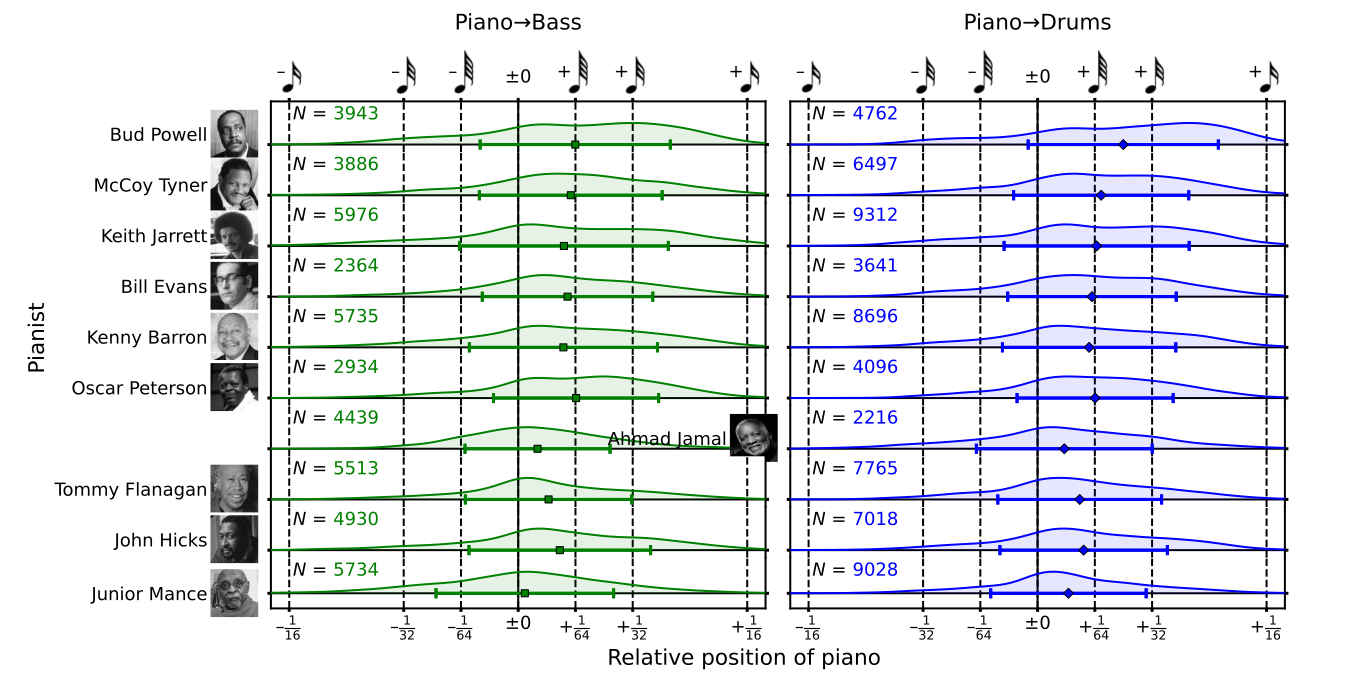
\includegraphics[width=1\textwidth]{figures/rsi_xai/figure_6.pdf}
  \caption[Piano rolls annotated with \GLS{LIME}.]{Piano rolls annotated with \GLS{LIME}. Both panels show a single clip from a performance by (a) Bill Evans and (b) Oscar Peterson. Highlighted in blue are the five areas of the piano roll that contribute the most towards predicting the target label. The asterisk in (a) indicates the descending arpeggio $(0, -4, -7, -11)$ pattern identified in Figure~\ref{fig:rsi_predictive_melody_features}.}
\label{fig:rsi_lime_plots_main}
\end{figure}

We use \GLS{LIME} to interpret test-split predictions made by the ResNet trained with augmentation. We use the default settings in the Python library (version \texttt{0.2.0.1}) provided by the authors of the original paper \citep{Ribeiro2016}. Figure~\ref{fig:rsi_lime_plots_main} highlights the four regions with the strongest \GLS{LIME} attributions (i.e., that push the model to positively identify the target class) for clips by Bill Evans and Oscar Peterson. Similar figures for clips by Abdullah Ibrahim, Chick Corea, and Keith Jarrett (the third, fourth, and fifth pianists with the greatest number of recordings: see Figure~\ref{fig:rsi_dataset}a) are provided in Figure~\ref{fig:rsi_sm_lime_plots}. 

The \GLS{LIME} technique does seem to emphasise musical gestures that could reasonably be considered distinctive for each performer. These include particular ascending and descending melodic patterns for Evans and several chord voicings for Peterson: interestingly, in the case of Evans, one of the attributed regions even contains the descending $(0, -4, -7, -11)$ arpeggio observed previously in Figure~\ref{fig:rsi_predictive_melody_features}a. Nonetheless, it is difficult to understand exactly what aspects of those gestures the model is paying attention to. Considering several of the scalar patterns highlighted for Evans, their explanatory power could reasonably derive from the intervallic structure of the scale, the harmony that it outlines, or the rhythmic and dynamic trends that shape it. Exactly which of these possibilities is the case is difficult to grasp, as all of these musical dimensions are entangled within the input \citep[see][]{Dervakos2022}.

\section{Multiple Input Representations Approach}\label{sec:rsi_factorised_inputs_approach}

One possible solution to this problem would be to extract a single high-level musical dimension from the original transcription and train a model with only this information. Melody, for instance, could be isolated by applying the skyline algorithm. However, isolating only a single musical dimension would likely reduce predictive accuracy, due to the model seeing less information than the original transcription. In addition, unless all other high-level musical dimensions are fixed, the model may exploit contextual ``shortcuts'' that do not encode the desired feature but instead those correlating with it \citep{Wei2024} --- such as increases in velocity appearing alongside an ascending melodic contour. 

Instead, in this section we outline a novel architecture that learns separate representations for four fundamental musical domains --- melody, harmony, rhythm, and dynamics \citep[see][]{Zhang2023-Horowitz} --- but then combines information from these four domains to make its predictions. Each domain is represented as a piano roll with the same shape as the original transcription. We then train small convolutional sub-networks to learn from each representation and aggregate the outputs together to generate a single feature vector that can be used to make predictions \citep[as in][]{Ramoneda2024}. 

This multi-\textit{input} architecture is different to the multi-\textit{task} learning approach described earlier by \citet{Velenis2023}, where a single input representation from a jazz ``lead sheet'' was used to generate multiple downstream predictions (for e.g., composer, tonality, form identification). Instead, our approach can be thought of as conceptually similar to a mixture-of-experts model without a gating network, allowing us to explicitly control the contribution of each input and sub-network (``expert'') towards a single downstream task (performer identification).

\subsection{Methods}\label{sec:rsi_factorised_methods}

\subsubsection{Input Representations}\label{sec:rsi_factorised_description}

Given a one-channel piano roll with the dimensionality $(88, 3000)$, we want to split this into four separate rolls, all with the same height and width but which contain the melodic, harmonic, rhythmic, or dynamic content from the input. While it would be possible to use different dimensions for each roll (for instance, representing each melody note using a single pixel), maintaining the same dimensionality ensures that each roll remains directly comparable to the original input and to one another (receiving, for instance, the same number of learnable parameters).

Similar to how $n$-grams were extracted for the handcrafted models (see Section~\ref{sec:rsi_handcrafted_feature_extraction}), to generate the melody representation we apply the skyline algorithm to the transcription to generate a vector of note events $M$. We remove velocity information from each note $m \in M$ by converting the channel dimension to binary, setting a value of 1 for when a note is played and 0 when it is not --- such that $m_{velocity}\in \{0, 1\}$. We remove rhythmic information by setting the inter-onset interval for each note to a constant value dependent on the length of M. Thus, 
\begin{align}
m_{on}^{i+1}-m_{on}^i = \dfrac{T}{|M|}, \ i \in \{1, 2, \dots, |M|\} \ ,
\end{align}
where $T$ is the width of the original input (i.e., 3,000). Note that, when $i = 1$, $m_{on} = 0$ and, when $i=|M|$, $m_{off}^{|M|} = T$. We then adjust the onset and offset times between successive notes to remove any overlap and maintain the original dimensionality of the input, such that $m_{on}^{i+1} = m_{off}^i$.

To generate the harmony representation, we quantise the transcription by grouping near-simultaneous notes into non-overlapping bins according to their onset time, with the size of each bin again set to 100 milliseconds as in Section~\ref{sec:rsi_handcrafted_feature_extraction}. This yields a vector of quantised bins $H$, where the size of every bin $|h| > 3$ for $h \in H$. Unlike the models trained on the handcrafted feature set (see Section~\ref{sec:rsi_handcrafted_feature_extraction}), however, we do not need to set an upper limit to the number of notes in the chord. We set the inter-chord interval for all notes in each bin to a consistent value, adjust the onset and offset times to remove any overlap between successive chords, and convert the channel dimension to binary.

To generate the rhythm representation, we want to maintain only the onset and offset times for every note $r$ in the original transcription. The influence of dynamics can be removed by converting the channel dimension to binary, as before. While it would be possible to remove the pitch dimension entirely as well, this could lead to situations where two notes with overlapping onset and offset times in the transcription are indistinguishable from each other in the derived representation. Instead, we randomise the pitch of each note $r$, such that $r_{pitch} \sim \mathcal{U}(21, 108)$, where $\mathcal{U}$ is a discrete uniform distribution of integers.

To generate the dynamics representation, we want to maintain only the velocity of each note in a transcription. We follow the process described to generate the harmony representation by binning near-simultaneous notes and adjusting their onset and offset times, but we do not set a lower boundary for the number of notes contained within a single bin (i.e., conceptually similar to the ``snap to grid'' function implemented in many commercial MIDI editors and digital audio workstations). Next, we randomise the pitch of each note in every bin. The representation derived from this process is thus the only one of the four used to train our model where the channel dimension of a note is a floating-point value, rather than an integer.

\subsubsection{Model Architecture}\label{sec:rsi_factorised_architecture}

Our proposed architecture uses four convolutional sub-networks to generate an $x$-dimensional embedding from every input roll. Each sub-network shares the same architecture, but the weights are updated separately. We test a range of architectures in our experiments, including 50-, 34-, and 18-layer ResNets --- the latter being the smallest implemented in \texttt{PyTorch}. We also test the \GLS{CRNN} architecture described in Section~\ref{sec:rsi_representation_methods}. As a form of regularisation, during training we experiment with masking the outputs of particular sub-networks with zeroes. There is a 10\% chance that one, two, or three sub-networks will be masked when processing a clip (i.e., a 30\% total probability of masking any number of sub-networks), with 70\% probability that all four sub-networks will be used during prediction.

\begin{figure}[!ht]
  \centering
  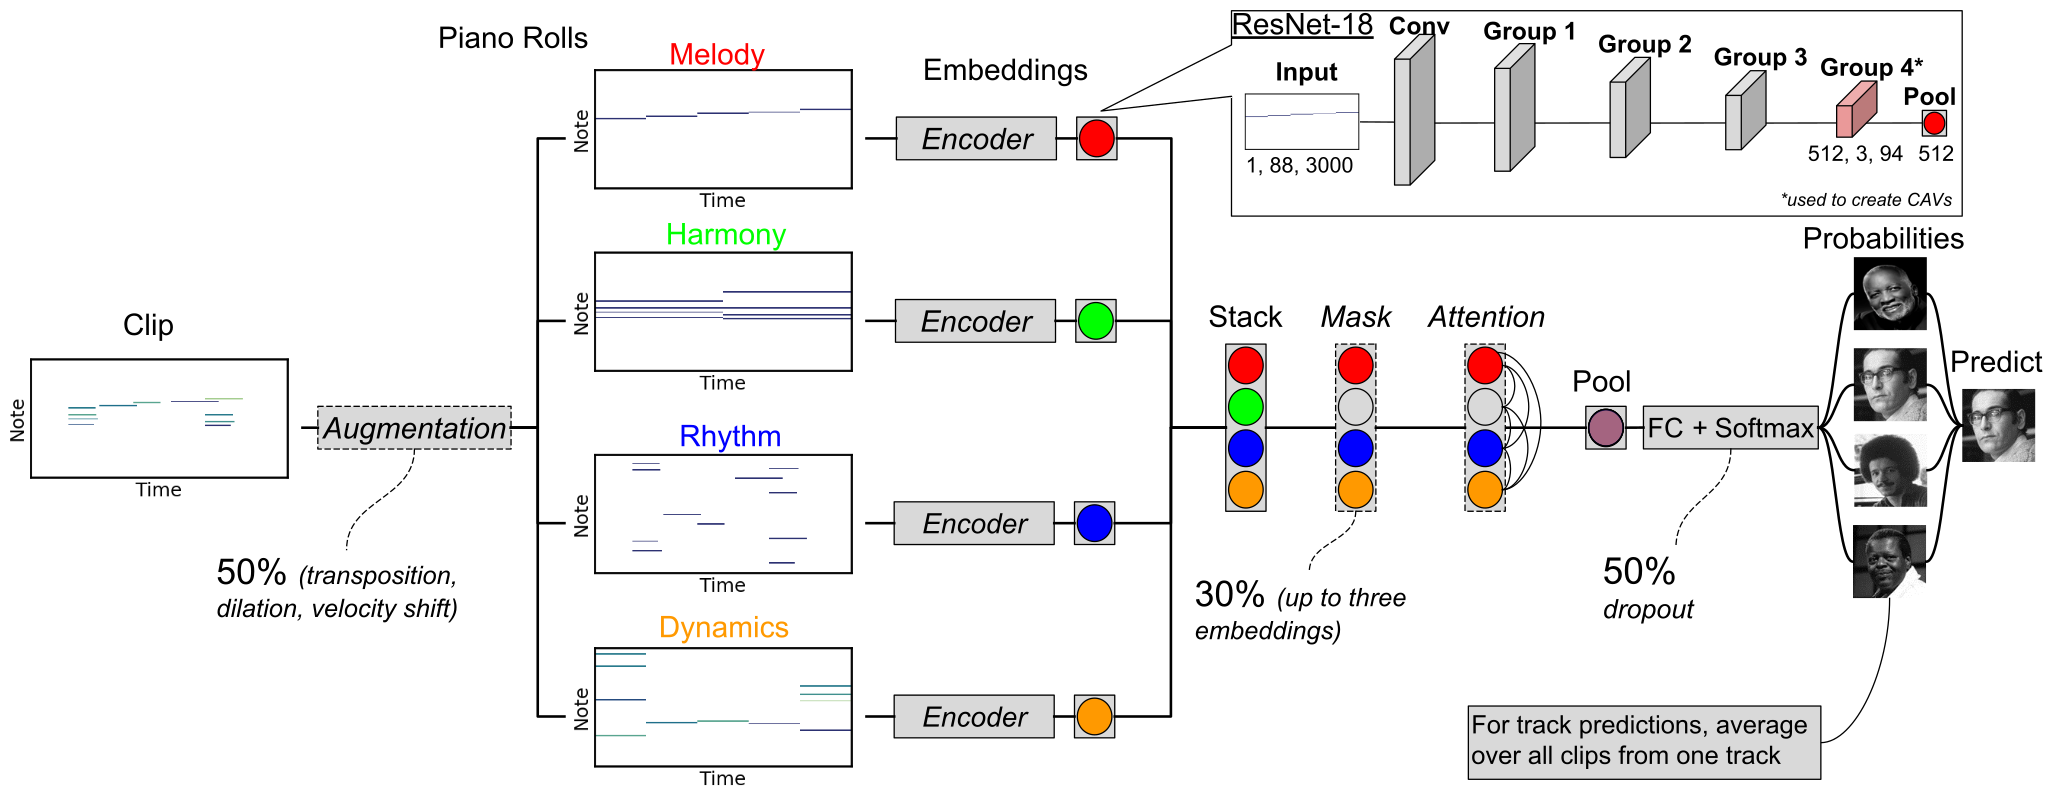
\includegraphics[width=1\textwidth]{figures/rsi_xai/figure_7.pdf}
  \caption[Proposed multi-input performer identification model architecture.]{Proposed multi-input performer identification model architecture. An input transcription is represented using four piano rolls, each relating to a musical domain. Each roll is processed with a separate sub-network, the embeddings are then pooled, and class probabilities are generated. The architecture of an 18-layer ResNet is shown here; different architectures are tested in our experiments (see Table~\ref{tab:rsi_factorised_input_experiment_results}). Optional components are represented with dashed lines.}
\label{fig:rsi_proposed_architecture}
\end{figure}

The outputs from each network are then stacked vertically to create an array with shape $(4, x)$. It would be straightforward to generate the final $x$-dimensional feature vector by either taking the average or maximum of the neurons in every ``column'' of this array. However, this might not be sufficient to allow the model to capture interactions between different musical domains. Consequently, we experiment with using a self-attention layer (with between four and sixteen heads) across embeddings prior to pooling. After aggregation, the resulting $x$-dimensional feature vector is fed into a fully connected layer (with dropout at a rate of 50\%) and softmax function to generate class probabilities. Figure~\ref{fig:rsi_proposed_architecture} shows an outline of the proposed architecture. Our best-performing multi-input model has a total of 44.7 million learnable parameters.

\subsubsection{Training}\label{sec:rsi_factorised_training}

We train the model for 100 epochs with a batch size of 20, using thirty-second clips and aggregating class probabilities to obtain track-level predictions. We use the Adam optimiser with categorical cross-entropy loss and a learning rate of 0.0001. Training takes between twelve and twenty-one hours on a single NVIDIA A100 SXM4 GPU, depending on the size of the model. We make a model card \citep{Mitchell2019} available on the same open source repository that contains the model code (see Footnote~\ref{note:rsi_webapp}).

\subsection{Results}\label{sec:rsi_factorised_results}

\subsubsection{Who is the Performer of an Unknown Musical Piece?}\label{sec:rsi_factorised_evaluation}

\begin{sidewaystable}[]
    \caption[Experiment results for models trained with multiple inputs.]{Experiment results for models trained with multiple inputs. Note that, when the number of attention heads is 0, self-attention is not used.}
    \label{tab:rsi_factorised_input_experiment_results}
    \centering
        \begin{tabular}{l c c c c c c}
        \toprule
        \textbf{Input Encoder} & \textbf{Attention heads} & \textbf{Pooling} & \textbf{Augmentation} & \textbf{Masking} & \multicolumn{2}{c}{\textbf{Accuracy} $\uparrow$} \\ \cmidrule{6-7}
        & & & & & \textbf{Clip} & \textbf{Track} \\
        \midrule
        \multicolumn{7}{c}{\textit{Network Architecture}} \\
        \midrule
        ResNet-18 & 0 & Average & Y & Y & \textbf{0.767} & \textbf{0.913} \\
        ResNet-34 & 0 & Average & Y & Y & 0.744 & 0.906 \\
        ResNet-50 & 0 & Average & Y & Y & 0.707 & 0.863 \\
        \GLS{CRNN} & 0 & Average & Y & Y & 0.622 & 0.812 \\
        \midrule
        \multicolumn{7}{c}{\textit{Self-Attention}} \\
        \midrule
        ResNet-18 & 4 & Average & Y & Y & 0.691 & 0.825 \\
        ResNet-18 & 8 & Average & Y & Y & 0.721 & 0.856 \\
        ResNet-18 & 16 & Average & Y & Y & 0.707 & 0.844 \\
        \midrule
        \multicolumn{7}{c}{\textit{Pooling}} \\
        \midrule
        ResNet-18 & 0 & Max & Y & Y & 0.753 & 0.906 \\
        ResNet-18 & 4 & Max & Y & Y & 0.683 & 0.831 \\
        \midrule
        \multicolumn{7}{c}{\textit{Data Augmentation \& Masking}} \\
        \midrule
        ResNet-18 & 0 & Average & N & Y & 0.644 & 0.789 \\
        ResNet-18 & 0 & Average & Y & N & 0.743 & 0.863 \\
        ResNet-18 & 0 & Average & N & N & 0.619 & 0.806 \\
        \bottomrule
        \end{tabular}
\end{sidewaystable}

The results for all experiments are shown in Table~\ref{tab:rsi_factorised_input_experiment_results}. We obtain the most accurate predictions of the held-out test recordings using the smallest ResNet with 18 layers; increasing the size of each sub-network beyond this decreases performance, which would suggest that overparameterisation occurs with larger architectures \citep{Zhang2023-Symbolic}. We find that accuracy does not improve with the addition of self-attention. This could imply that there are no meaningful interactions between the different musical domains as they are represented here. As the network has only a single fully connected layer, this would instead imply that the contributions of each sub-network are additive. Finally, we observe slight performance improvements from using masking.

Compared with the other models described here, our proposed architecture using multiple inputs achieves impressive accuracy in identifying twenty jazz pianists. For instance, it almost matches the performance of the ResNet trained with augmentation on a unified piano roll representation (0.913 vs. 0.944 accuracy). There is therefore some trade-off between interpretability and predictive performance, at least in our case; however, it is impressive that the multi-input model can nearly match the state-of-the-art in this task.

\subsubsection{Which Domains are Important for Musical Style?}\label{sec:rsi_factorised_domain_importance}

\begin{figure}[!ht]
  \centering
  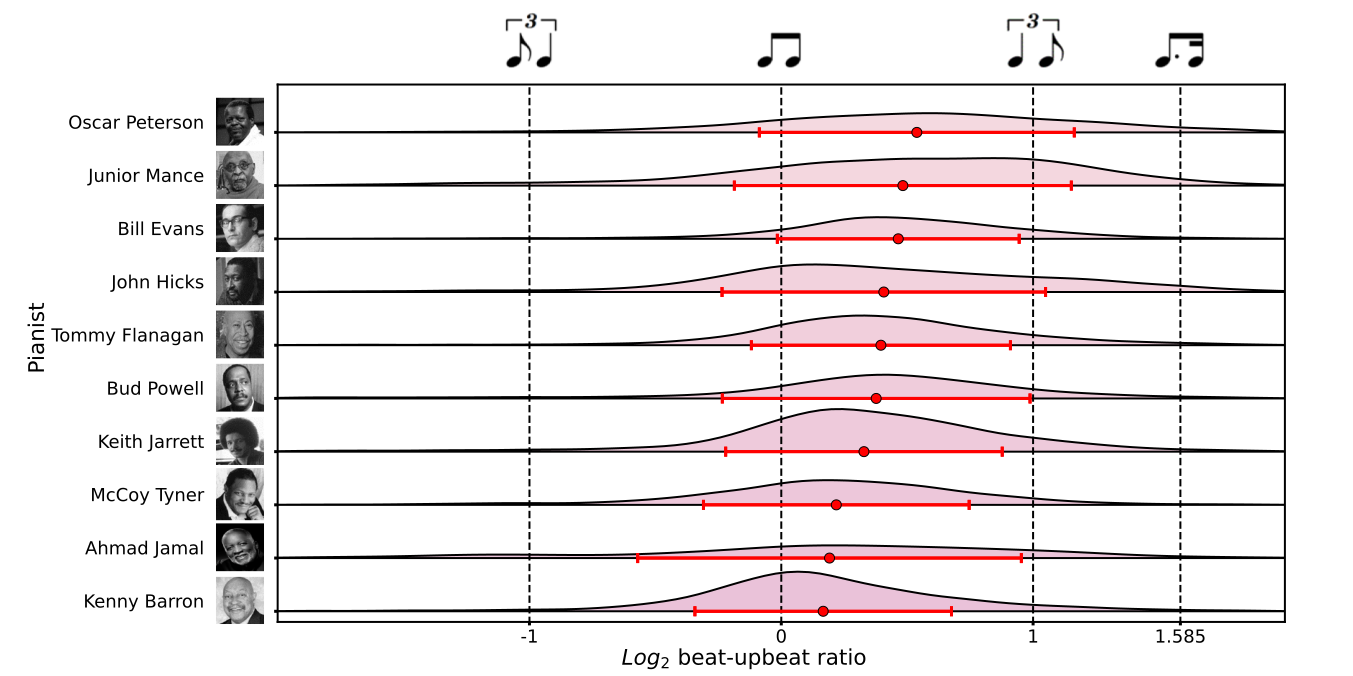
\includegraphics[width=1\textwidth]{figures/rsi_xai/figure_8.pdf}
  \caption[Multi-input performer identification model, musical domain masking.]{Multi-input performer identification model, musical domain masking. (a) shows the loss in accuracy compared with the full model when masking a single sub-network. (b) shows the accuracy of predictions made using only a single sub-network. The dotted lines in (b) show the accuracy from predicting the majority class and the accuracy of the ``full'' model (using all four sub-networks).}
\label{fig:rsi_factorised_evaluation}
\end{figure}

There are at least two ways to evaluate these high-level musical domains. The first considers how important each representation is to the full model by computing the loss in accuracy when the output of a single sub-network is masked with zeroes (Figure~\ref{fig:rsi_factorised_evaluation}a). Masking either the melody, rhythm, or harmony sub-network leads to a small, relatively consistent drop in accuracy, with the greatest loss observed for rhythm (rhythm accuracy loss: $-0.069$, melody: $-0.063$, harmony: $-0.056$). Masking the output of the ``dynamics'' sub-network leads to a considerably smaller loss in accuracy, however ($-0.019$), which suggests that dynamics are relatively unimportant when predicting the improvisation style of a jazz pianist. 

\begin{figure}[!ht]
  \centering
  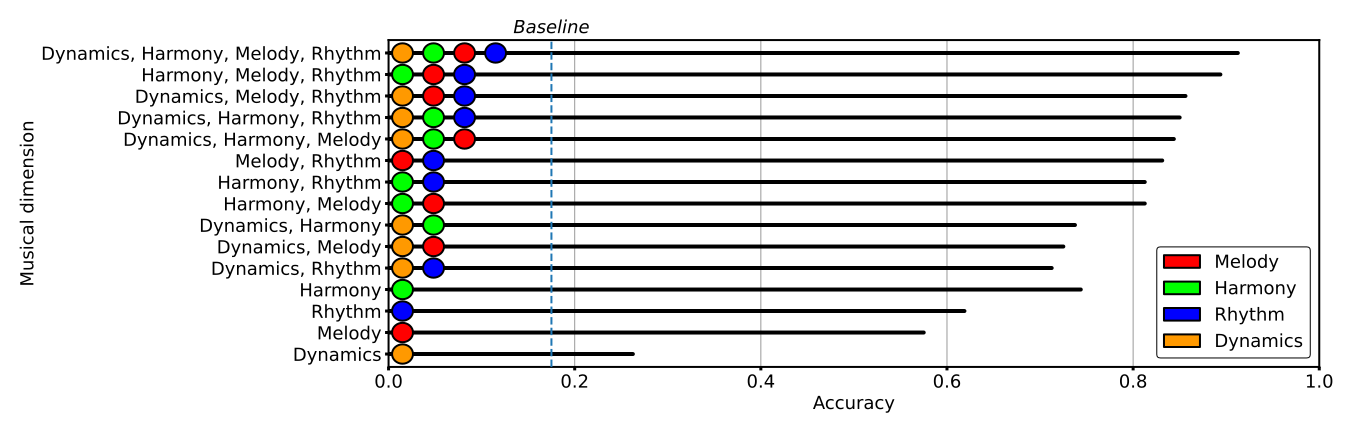
\includegraphics[width=1\textwidth]{figures/rsi_xai/figure_s43.pdf}
  \caption[Multi-input performer identification model evaluation.]{Multi-input performer identification model evaluation. The ``lollipop'' plot shows the accuracy obtained from predicting using all combinations of sub-networks, with the coloured ``heads'' of each lollipop indicating the particular networks used to make the predictions. The dotted ``baseline'' score is the accuracy obtained from a model that simply predicts the majority class for every recording.}
\label{fig:rsi_sm_factorised_lollipop}
\end{figure}

A second way to consider the importance of each domain is to compute how well a single representation predicts by itself, when the output of the other three sub-networks is masked (Figure~\ref{fig:rsi_factorised_evaluation}b). As before, predictive accuracy is lowest when using only the dynamics sub-network (0.263 accuracy) --- and is only slightly better than a model which simply predicts the majority class. Both melody and rhythm sub-networks yield similar predictive accuracy (0.575 and 0.619, respectively). The most accurate predictions are obtained using only the harmony sub-network, with nearly three-quarters of unseen recordings being classified correctly (0.744). We show the predictive accuracy obtained for all combinations of sub-networks in Figure~\ref{fig:rsi_sm_factorised_lollipop}.

The importance of melodic content for distinguishing between different improvising jazz musicians has been demonstrated previously in the computational modelling literature \citep{Frieler2016, Weis2018}. The same is true, also, for rhythm, with \citet[pp. 86-88]{Benadon2006} noting how ``expressive features of `time feel' serve to define the stylistic profile of [particular] jazz musicians'' (see also Chapter~\ref{chap:rhythm_rsos}). Finally, that harmony should be particularly indicative of performance style is perhaps unsurprising: in his monograph on jazz style, Mark \citet[p. 95]{Gridley1994} describes how ``each pianist's particular approach to ... chording [is] a signature for [their] style''.

An interesting discrepancy here is that harmony is seemingly the most predictive domain when used on its own, while rhythm is the most important when all other domains are included. One possible interpretation could be that some melodic information bled into the harmony representation, and vice-versa. As we did not remove the output of the skyline algorithm before extracting chords (see Section~\ref{sec:rsi_handcrafted_feature_extraction}), there could be a degree of overlap between the features learned by the harmony and melody sub-networks. This is difficult to avoid, however, as the top note of any chord can theoretically have both a harmonic and melodic function in jazz \citep{Levine2011}.

\subsubsection{Which Domains Best Distinguish Particular Performers?}\label{sec:rsi_performer_domain_distinctiveness}

\begin{figure}[!ht]
  \centering
  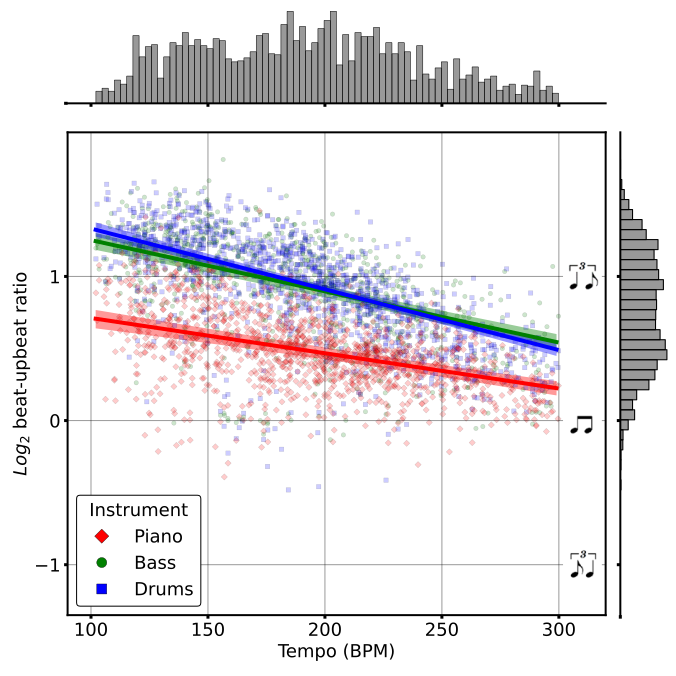
\includegraphics[width=1\textwidth]{figures/rsi_xai/figure_9.pdf}
  \caption[Multi-input model, class accuracy per musical domain.]{Multi-input model, class accuracy per musical domain. Each facet shows the percentage of recordings in the held-out test split classified correctly for each pianist when predicting using only a single sub-network.}
\label{fig:rsi_class_accuracy_per_domain}
\end{figure}

\begin{figure}[!ht]
  \centering
  \includegraphics[width=1\textwidth]{figures/rsi_xai/figure_s44.png}
  \caption[Multi-input model, class accuracy across musical domains.]{Multi-input model, class accuracy across musical domains. Each facet contains a heatmap showing the probability that, when given a recording and the output from a sub-network, the model will identify a particular pianist. The proportion of hits is shown for each facet along the diagonal; all other values are misses. Lighter and darker colours indicate lower and higher predictive probability, respectively.}
\label{fig:rsi_sm_factorised_heatmap}
\end{figure}

In Figure~\ref{fig:rsi_class_accuracy_per_domain}, we show the per-class accuracy for predictions made using a single sub-network, which allows us to consider the degree to which particular domains best distinguish individual performers. The 22 held-out recordings by Bill Evans, for instance, can be predicted with 0.964 accuracy using only the harmony sub-network. In his description of Evans' improvisation style, Brian Priestley \citep[p. 159]{Carr1988} notes that ``his left-hand [chord] voicings were utterly distinctive although universally imitated''. Related to this is how numerous pianists --- all of whom were born after Evans --- are misclassified by our model as Evans when predicting with only the harmony sub-network (Figure~\ref{fig:rsi_sm_factorised_heatmap}). For Ted \citet[p. 275]{Gioia2011}, Evans' voicings ``almost serv[ed] as a default standard among later pianists''. Several of the pianists frequently misidentified as Evans have directly cited him as an influence, including Keith Jarrett \citep{Jarrett2009}.

Our results also suggest that several musicians are particularly distinctive for their use of rhythm. This includes Kenny Barron and Chick Corea, as all of their recordings in the held-out test set can be correctly classified solely using the rhythm sub-network, with considerably lower accuracy obtained when using only the harmony sub-network (0.800 for Kenny Barron, 0.714 for Chick Corea). A possible explanation could be that Corea is one of the only pianists in our dataset to have extensively recorded Latin American music \citep{Gioia2011}. The distinctiveness of every domain for each performer can be explored as part of our interactive web application (see Footnote~\ref{note:rsi_webapp}, subheading ``style'').

However, we also note that the performers distinguished most accurately using the rhythm sub-network of our multi-input model differ from those identified by the model we go on to describe in Chapter~\ref{chap:rhythm_rsos}. As we shall see, this model is trained on a handcrafted set of rhythmic features derived from prior empirical writings on jazz, such as swing ratio and onset density. There are nine performers in common between the datasets used to train both models. Ranking the accuracy of classifications for these performers and then correlating the ranks demonstrates little connection between the performers that can be distinguished solely using rhythm ($r = -0.296$). One possibility is that the handcrafted model averages features across an entire recording to produce a global value, while our multi-input model may instead have learned to pick up on more local rhythmic features. Another is due to differences in the methods used to extract the data used to train both models (see Section \ref{sec:jtd_alternate_methods}).

\subsubsection{What is the Most ``Characteristic'' Example of a Performer's Style?}

Our web application also allows the user to listen to a single example deemed most ``distinctive'' for a given combination of performer and musical domain (e.g., which recording demonstrates the most ``Bill Evans-like'' melodic lines?). This is established by finding the clip from the held-out test set that maximises the logits for the target class when predicting using each of the four sub-networks individually. 

Listening to some of these examples, we can speculate that our multi-input model may indeed have learned to pick up on some of the same features discovered by our handcrafted model (see Section~\ref{sec:rsi_feature_importance_by_performer}). For instance, the most ``distinctive'' melody clip for Bill Evans includes many of the arpeggio figurations contained in Figure~\ref{fig:rsi_predictive_melody_features}a; likewise, the most distinctive harmony clip contains some of the ``rootless'' voicings shown in Figure~\ref{fig:rsi_sm_evans_harmony}.

\subsubsection{Which Features are Associated With Particular Performers?}\label{sec:rsi_factorised_cavs}

\begin{figure}[!ht]
  \centering
  \includegraphics[width=1\textwidth]{figures/rsi_xai/figure_s45.png}
  \caption[Concept activation vector examples.]{Concept activation vector examples. The musical notation shows an example exercise taken from the ``Modal Fourthy Voicings'' section in \citet[p. 52]{Haerle1994}.}
\label{fig:rsi_sm_haerle_example}
\end{figure}

Finally, we can relate the features learned by our model to a set of music-theoretic concepts extracted from a textbook used widely in jazz education \citep{Haerle1994} in order to understand how these might manifest in each performer's playing. This book comprises twenty chapters, with each chapter containing multiple exercises that demonstrate a single harmonic concept or progression --- beginning with simple ideas (``Block Chords'', ``Diatonic 7th Chords'') and progressing to more complex ones by the end (``Tritone II-V-Is'', ``Dominant Polychord Groups''). For a complete description of each chapter, see Table~\ref{tab:rsi_sm_haerle_concepts}. We reproduce a single exercise from this book in Figure~\ref{fig:rsi_sm_haerle_example}.

To relate these exercises to the model's predictions, we use concept analysis techniques initially developed for computer vision \citep{Kim2018} and more recently applied to classical music composer identification \citep{Foscarin2022}. To summarise, this method works by using ``activation vectors'' that represent the contributions of human interpretable concepts \citep[e.g., difficult-to-play music, contrapuntal textures in][]{Foscarin2022} to explain a model's decision after it has been trained. Unless stated otherwise, our methods follow those given in \citet{Foscarin2022}.

We derive our concepts from the exercises in each chapter, transposed to C minor/major. As data augmentation, we include versions of each exercise with (1) all possible transpositions up to $\pm 6$ semitones, (2) all possible inversions, and (3) both root and ``rootless'' forms. These exercises are represented in the same two-dimensional piano roll format as used to train our harmony sub-network (see Section~\ref{sec:rsi_factorised_description}). We compute the activations for an exercise by flattening the output of the final layer of this sub-network (``Group 4'', Figure~\ref{fig:rsi_proposed_architecture}) from the best-performing multi-input model into a one-dimensional representation with shape $(C \times H \times W)$.

Next, we train binary logistic regressions to separate the activations for one concept with those from a random dataset, consisting of an equivalent number of exercises sampled randomly across every other chapter in Haerle's book. We then take a clip from either the validation or test split of the dataset and score its sensitivity to a concept by taking the dot product of the layer activations with the corresponding concept activation vector. Finally, we define the sign-count ratio for a given performer and concept as the proportion of their clips for which the score is positive. If the sign-count ratio is greater than 0.5, this suggests that this concept encourages the classification of the performer; vice-versa, a sign-count ratio below 0.5 suggests that it discourages classification.

\begin{figure}[!ht]
  \centering
  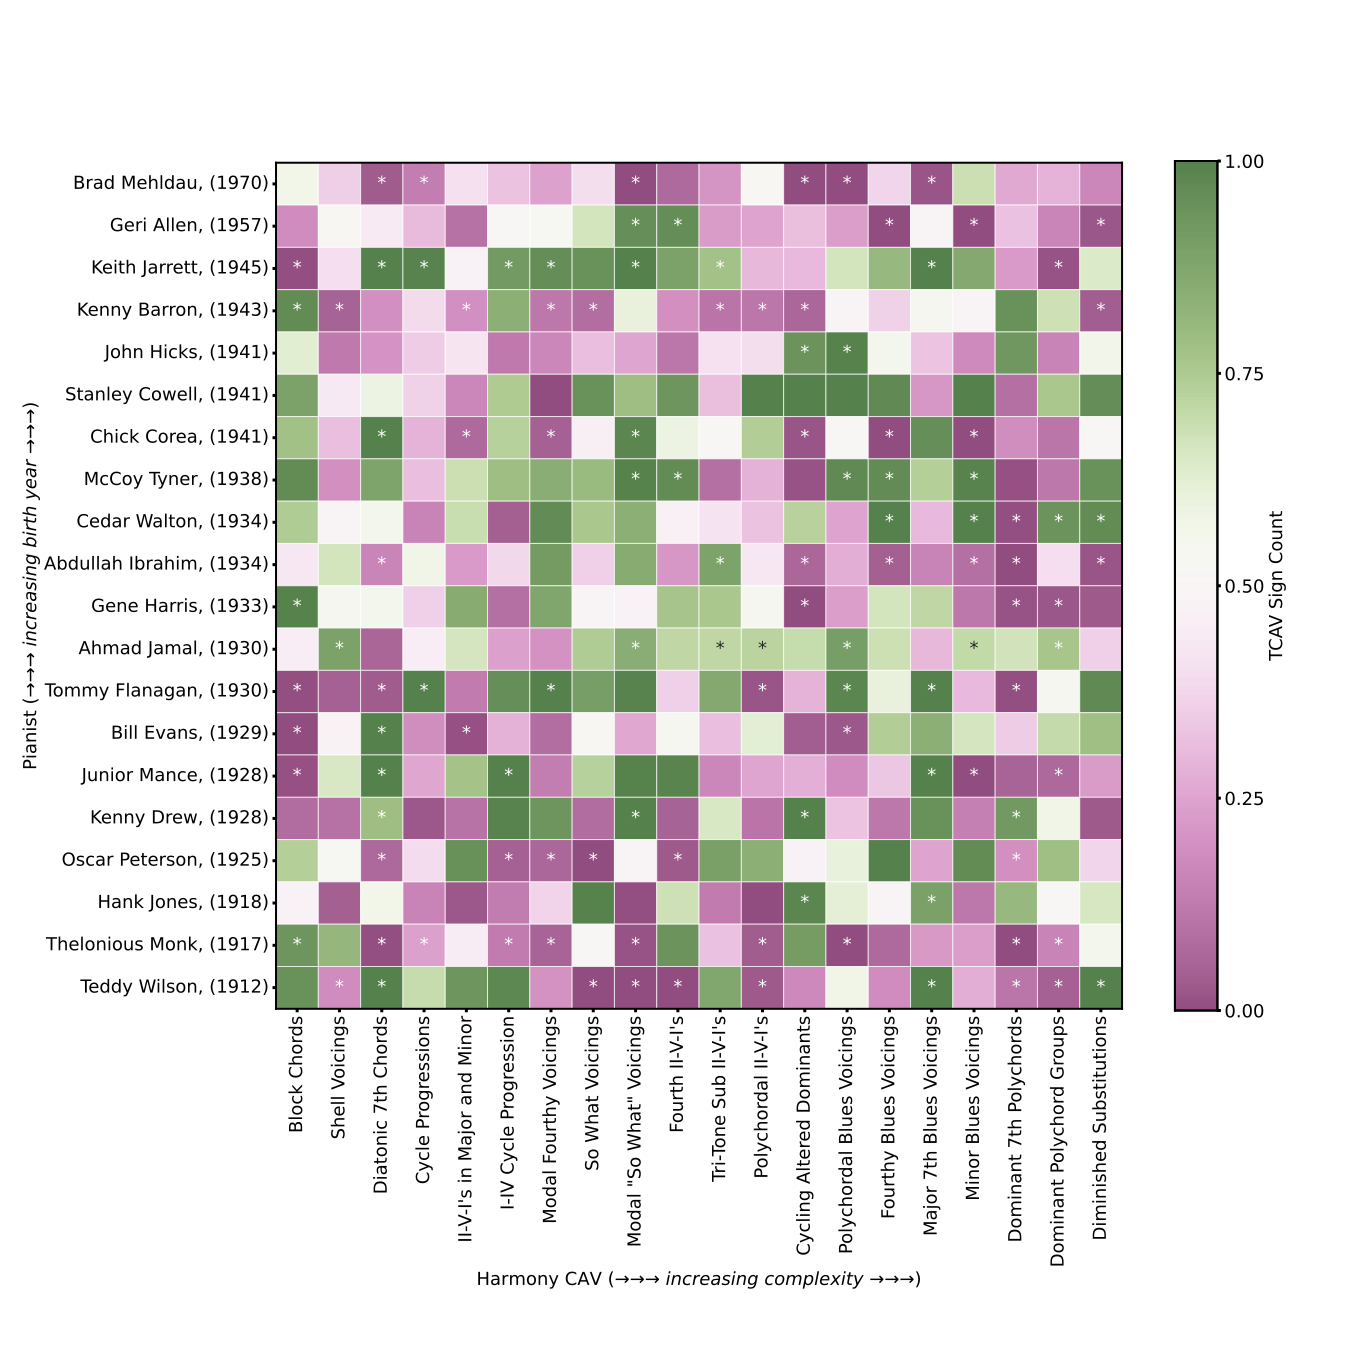
\includegraphics[width=1\textwidth]{figures/rsi_xai/figure_10.pdf}
  \caption[Concept sensitivity heatmap.]{Concept sensitivity heatmap. The heatmap shows the mean sign-count scores obtained for each performer ($y$-axis) to every harmonic concept ($x$-axis). The dendrograms show the results of applying agglomerative hierarchical clustering on the sign-count scores within each ``column'' or ``row''; pianists or concepts joined at lower positions are estimated to be more similar to those joined at higher values. Darker green colours indicate a positive influence of a concept on the classification of a performer; darker purples show negative influence. Asterisks show the significance of the sign-count scores ($^* \ p < .05$).}
\label{fig:rsi_cav_sign_counts}
\end{figure}

For every concept, we compute $N$ sign-count ratios for each performer by fixing the concept dataset and drawing a new random dataset for every iteration. We then obtain a null distribution of $N$ sign-count ratios for each performer by performing an equivalent analysis using two non-overlapping random datasets. We set $N = 10$, as in \citet{Foscarin2022}. We then perform a two-sided hypothesis test (Wilcoxon sign-rank) for every performer and concept and apply Bonferroni correction to control the false discovery rate on the performer level, with the number of hypotheses set to the number of concepts (i.e., 20). We show the mean sign-count ratio for each pianist and concept in Figure~\ref{fig:rsi_cav_sign_counts}. 

A number of observations can be made from this analysis. For instance, Brad Mehldau --- the youngest pianist in the dataset --- cannot positively be associated with any concept, which could suggest that contemporary jazz harmony draws from progressions not covered in Haerle's book. Indeed, several of the voicings most strongly associated with Mehldau by the model described in Section~\ref{sec:rsi_handcrafted_features_approach} consist of inversions of simple triads without any extensions, such as $(0, 8, 15)$: here, see Figure~\ref{fig:rsi_sm_mehldau_harmony}. These are not included in any of Haerle's chapters. John Hicks is associated with both the ``Cycling Altered Dominants'' and ``Dominant 7th Polychords'' concept. For Hicks, conceptualising ``two chords a tritone apart'' as a means to alter a dominant seventh by adding a sharpened eleventh and flattened ninth --- the same type of voicing contained within these concepts --- reportedly gave him ``a new freedom'' in his playing \citep[p. 160]{Berliner1994}.

Yet there are also some surprising results. Thelonious Monk is negatively associated with the ``Dominant 7th Polychords'' concept; yet, for Gunther \citet[p. 231]{Schuller1965}, it is in the use of such chords that Monk was ``one of the most imaginative innovators'' in jazz. Equally unexpected is that Bill Evans is not associated with concepts based on the ``So What'' chord voicing, despite himself being the originator of this voicing in work with trumpeter Miles Davis \citep{Gioia2011}. Similarly, Junior Mance was ``known principally for [his] highly ... bluesy approach'' \citep[p. 319]{Carr1988}, but is negatively associated with the ``Minor Blues Voicings'' concept.

These cases should be interpreted with caution, however. Just because the classifier does not consider a particular concept relevant for a musician does not mean that this is not present in their work \citep{Foscarin2022}. While Haerle's book is a comprehensive overview of jazz harmony it is not exhaustive, and there are ways (for instance) to create ``Blues-y'' sounding voicings that are not covered in this book \citep[see, for instance, the method adopted in][]{Adegbija2023}. Another possibility is that our dataset only considers trio and solo improvisations: Evans may have used the ``So What'' voicing primarily during his quintet recordings with Davis, for example.

To validate our pipeline, we can also use a masking technique to visualise which parts of a performance contribute most to a concept. We compute the original concept score $S_{x, y}$ as 
\begin{align}\label{eq:rsi_sm_cav_calculation}
S_{x, y} = f(x) \circ y \ .
\end{align}
Here, $x$ is a MIDI piano roll with input size $(88, 3000)$, $f$ transforms $x$ into layer activations with shape $(C \times W \times H)$, and $y$ is the vector of coefficients (with the same shape) extracted from a binary classifier trained to separate concept activations from random activations. 

We then slide a two-dimensional rectangular kernel with shape $(24, 250)$ (i.e., 2 octaves, 2.5 seconds) and stride $(2, 200)$ over $x$ and remove all MIDI notes with onset times contained within the span of the kernel. This produces the masked piano roll $x'$. We can then compute the masked concept score $S'_{x', y}$ and express this with relation to the original score:
\begin{align}
S_{x', y} = \frac{S_{x, y} - \biggl(f(x') \circ y \biggr)}{S_{x, y}}
\end{align}
Finally, after computing $S_{x', y}$ at every kernel position, we transform the result back into a two-dimensional image with the same shape as $x$ using linear interpolation.

\begin{figure}[!ht]
  \centering
  \includegraphics[width=0.9\textwidth]{figures/rsi_xai/figure_s46.png}
  \caption[``Tivoli'' (1991) transcription.]{`Tivoli'' (1991) transcription. The musical notation shows a transcription of the final 30 seconds from an unaccompanied performance by McCoy Tyner (``Tivoli'' from ``Soliloquy'', recorded in 1991, originally composed by Dexter Gordon). Transcription created by the author.}
\label{fig:rsi_sm_tivoli_transcription}
\end{figure}
\FloatBarrier\clearpage

\begin{figure}[!ht]
  \centering
  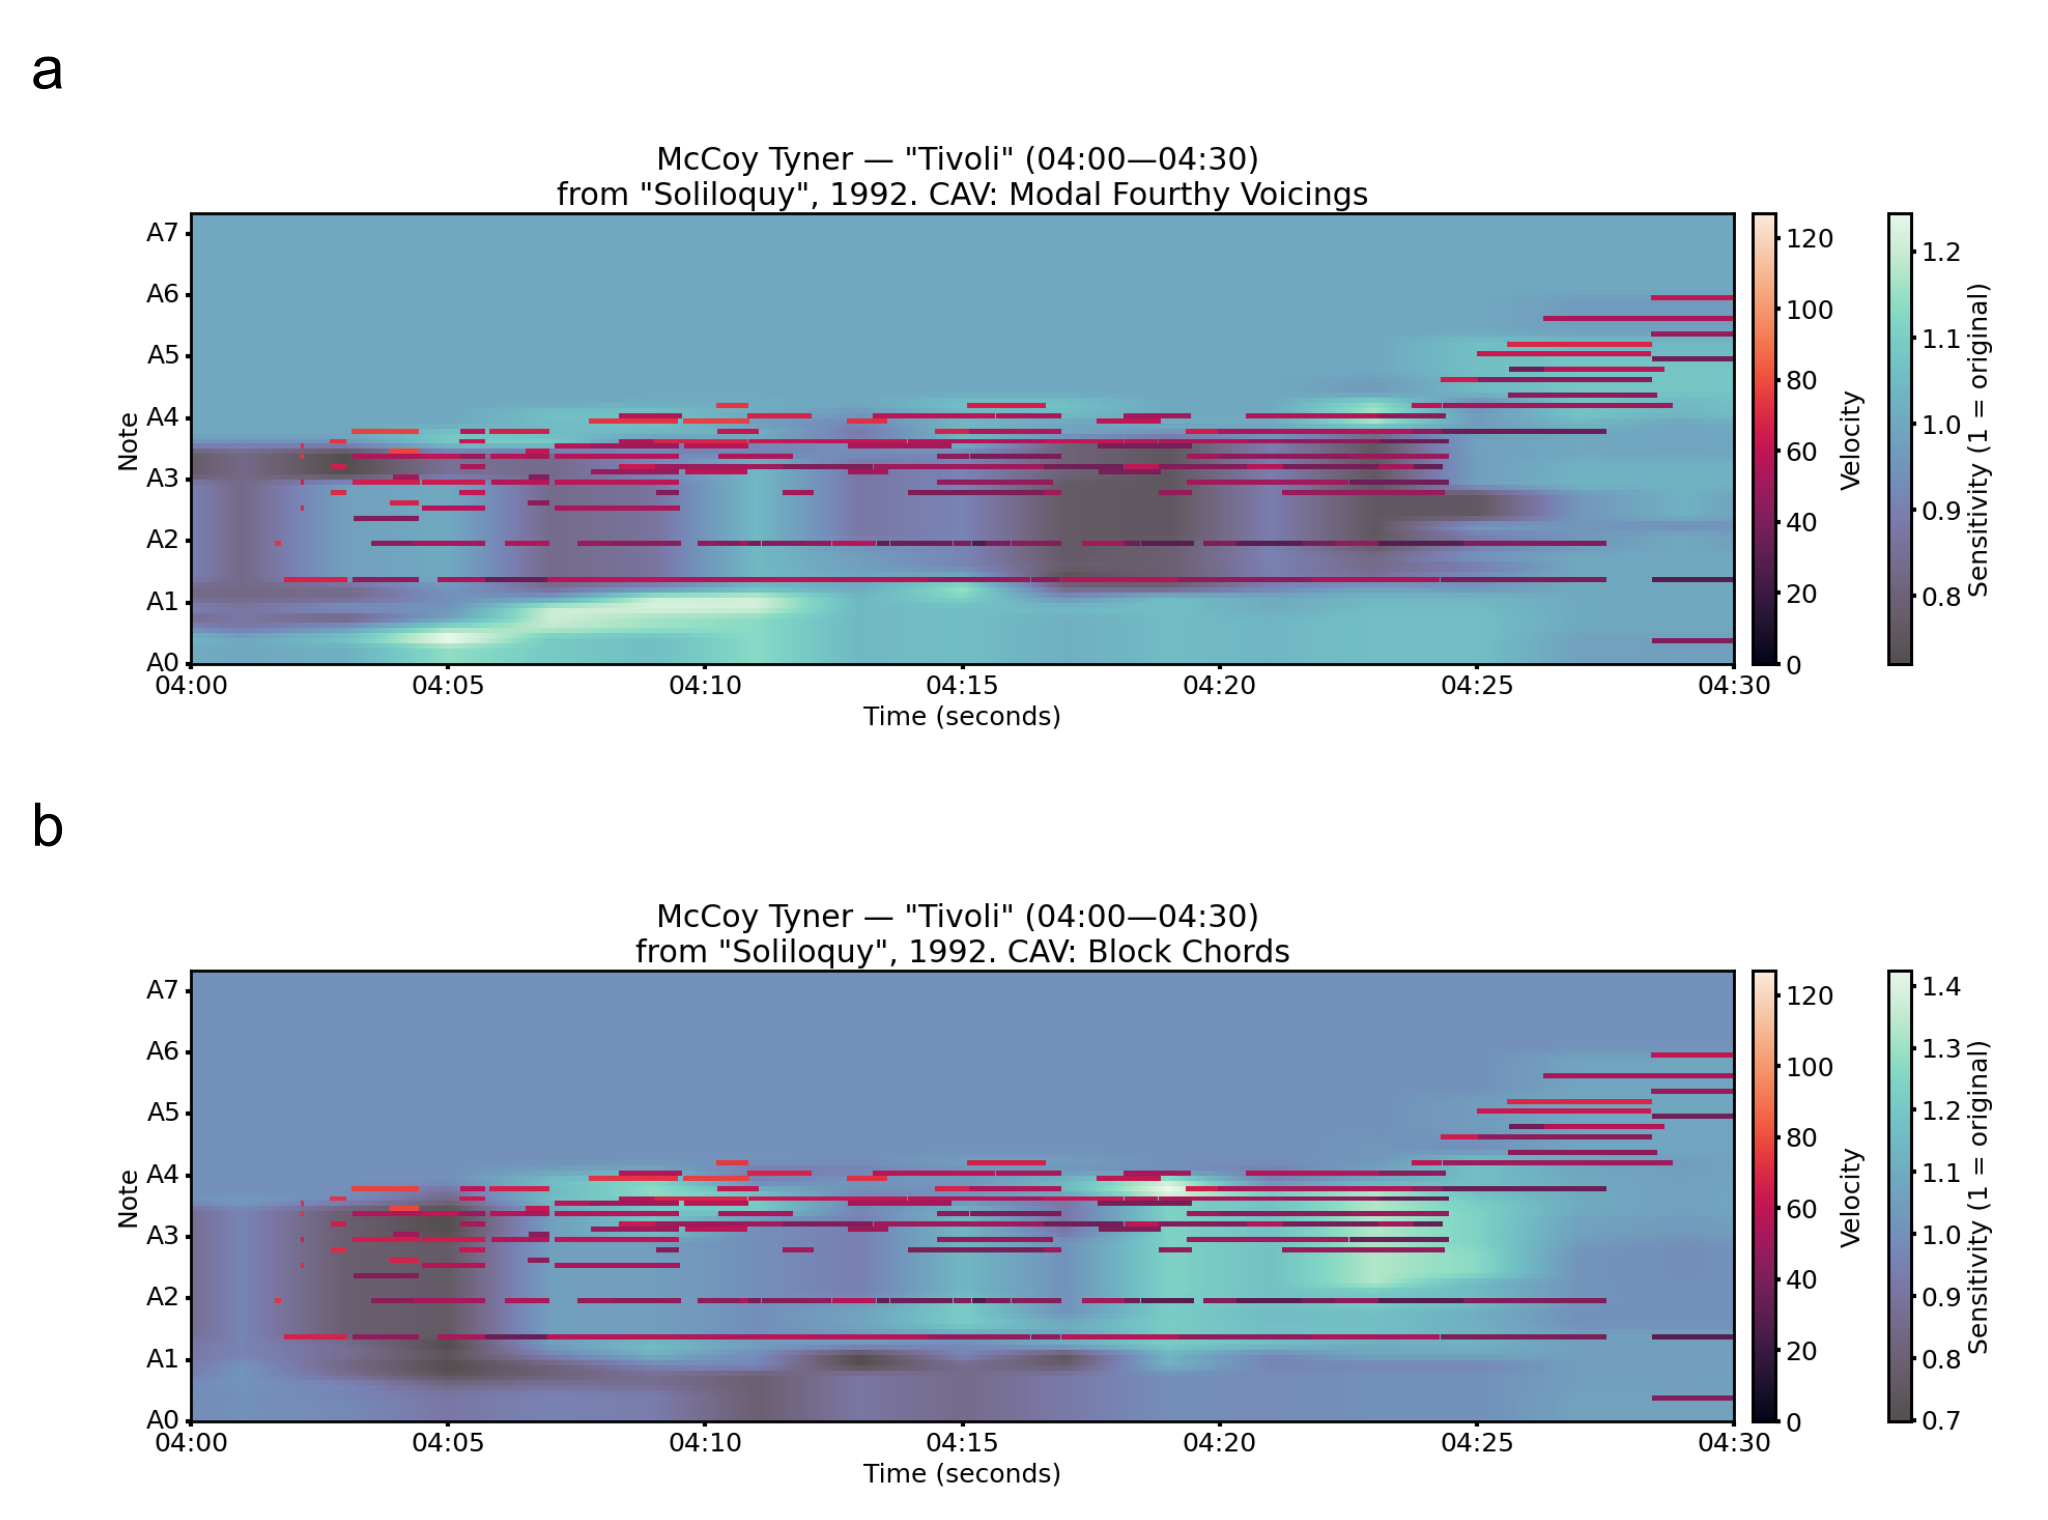
\includegraphics[width=1\textwidth]{figures/rsi_xai/figure_12.pdf}
  \caption[Visualising changes in concept score with masking.]{Visualising changes in concept score with masking. Each panel contains a MIDI piano roll with a heatmap overlaid to show the change in score to the (a) ``Modal Fourthy Voicings'' and (b) ``Block Chords'' concepts. Intuitively, green coloured sections contribute positively to the score calculated between the clip and the concept (i.e., they ``embody'' the target concept) and blue coloured sections contribute negative to the score. Values are scaled such that 0 is equivalent to the original score, calculated without masking. Musical notation is provided in Figure~\ref{fig:rsi_sm_tivoli_transcription}.}
\label{fig:rsi_tivoli_cav}
\end{figure}

Figure~\ref{fig:rsi_tivoli_cav} shows how the score calculated between a clip and the ``Modal Fourthy Voicings'' concept is based on the appearance of stacked, parallel fourth intervals. The same sections of this clip are not sensitive to the ``Block Chords'' concept, which involves chords based on stacked third intervals. Musical notation for this excerpt is given in Figure~\ref{fig:rsi_sm_tivoli_transcription}. We make interactive versions of these figures available for many other performances and concepts as part of our web application (see Footnote~\ref{note:rsi_webapp}, subheading ``harmony'').

\subsubsection{How are the Styles of Particular Performers Related?}\label{sec:rsi_cav_clustering}

\begin{figure}[!ht]
  \centering
  \includegraphics[width=1\textwidth]{figures/rsi_xai/figure_s47.pdf}
  \caption[Pairwise correlations between pianists.]{Pairwise correlations between pianists. The colour of each cell shows the strength of the linear relationships (Pearson's $r$) between sign-count ratios obtained between performers along the $x$- and $y$-axis. Darker reds and blues indicate stronger positive and negative associations, respectively. Sign-count ratios are collected for all concepts ($N = 20$) and across all iterations ($N = 10$) of the testing process, such that the total number of values considered for each pianist in every correlation is 200.}
\label{fig:rsi_sm_pianist_correlations}
\end{figure}

Finally, we relate the harmonic style of each performer using agglomerative hierarchical clustering. We compute the correlation coefficient $r$ between the sign-count ratios obtained for two performers across all concepts (i.e., $N = 200$: see Figure~\ref{fig:rsi_sm_pianist_correlations}), transform this into a distance matrix by taking $1 - r$, and perform hierarchical clustering using the mean inter-cluster dissimilarity to link performers together (see also Section~\ref{sec:rsos_rhythm_characterises_style}). A dendrogram created from this analysis is shown above the heatmap in Figure~\ref{fig:rsi_cav_sign_counts}. 

The final split in the dendrogram partitions the pianists into two groups containing nine and eleven musicians, respectively. The pianists in group 1 are associated more frequently with chords based on fourths (e.g., ``Modal `So What' Voicings'', ``Modal Fourthy Voicings''). McCoy Tyner and Chick Corea are included in this group (see Figures~\ref{fig:rsi_sm_tyner_harmony},~\ref{fig:rsi_sm_corea_harmony}). Vice-versa, the pianists in group 2 are instead associated with altered and extended chords (e.g., ``Cycling Altered Dominants'', ``Polychordal Blues Voicings''). Cedar Walton and John Hicks are included in this group (see Figures~\ref{fig:rsi_sm_walton_harmony} and~\ref{fig:rsi_sm_hicks_harmony}).

\begin{figure}[!ht]
  \centering
  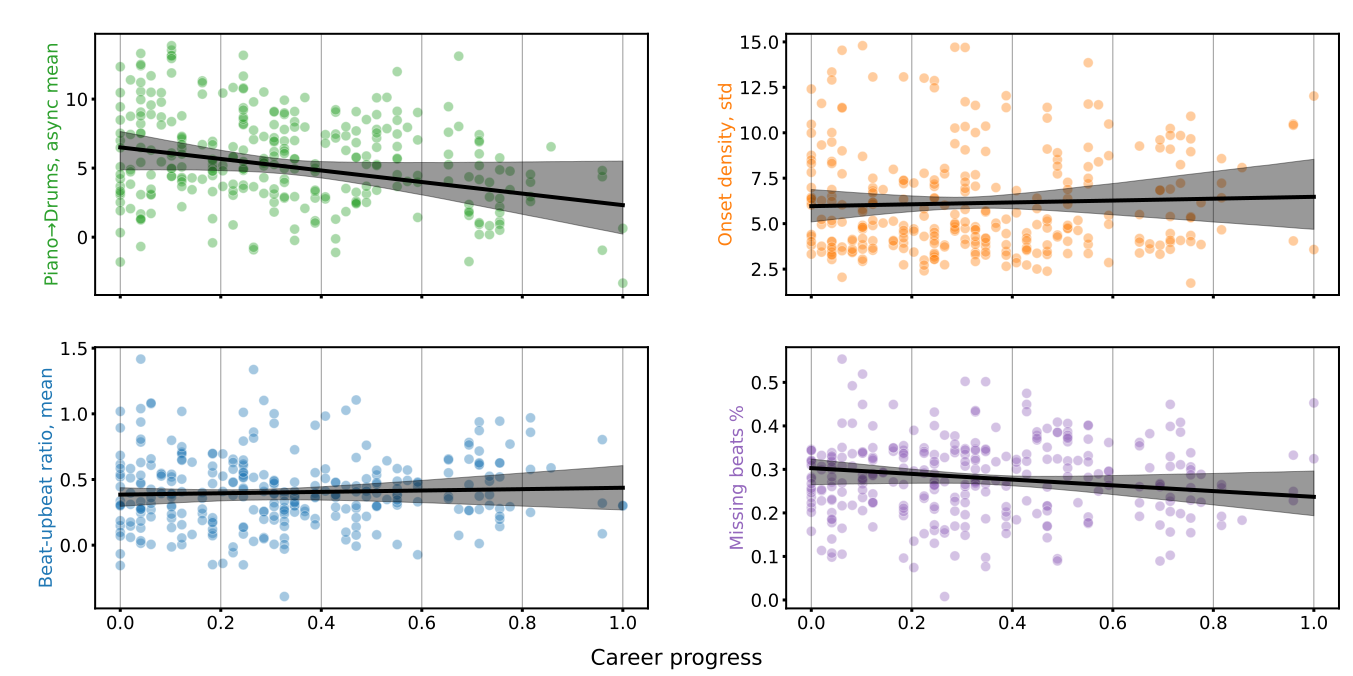
\includegraphics[width=1\textwidth]{figures/rsi_xai/figure_11.pdf}
  \caption[Pairwise correlations between musical concepts.]{Pairwise correlations between musical concepts. Sign-count ratios are collected for all performers ($N = 20$) and across all iterations, such that the total number of values considered for each concept in every correlation is 200.}
\label{fig:rsi_sm_cav_correlations}
\end{figure}

We can also apply the clustering technique to all of the sign-count ratios obtained for each individual concept, rather than each pianist (see Figure~\ref{fig:rsi_sm_cav_correlations}). Concepts with inherent musical similarities --- e.g., ``Fourth II-V-Is'' and ``So What Voicings'' (both based on the perfect fourth interval), and``Fourthy Blues Voicings'' and ``Minor Blues Voicings'' (both based on the twelve-bar blues progression) --- are clustered together earlier than those with contrasting harmonic constructions --- e.g., ``Block Chords'' and ``Modal `So What' Voicings'' (built on stacked third and fourth intervals, respectively). A dendrogram from this analysis is shown on the right of the heatmap in Figure~\ref{fig:rsi_cav_sign_counts}.

\section{Discussion}\label{sec:rsi_discussion}

The purpose of this chapter was to consider how machine learning can help deconstruct the ``style'' of individual artists --- the signature elements that make their work recognisable and distinct. We focussed on musical style (and jazz in particular), owing to the richness of critical literature on the subject and the fact that musicians commonly refer to many of these same theoretical concepts. We trained a series of supervised learning models to identify the performer on 84 hours of recordings made by twenty iconic jazz pianists and interpreted their decision-making processes \textit{post hoc}. Models we trained using handcrafted input features proved to be both accurate and interpretable, capable of answering questions relating both to the distinctiveness of high-level musical domains (harmony, melody) and local musical features (particular melodic patterns and chord voicings). Models we trained to learn representations directly from an input proved highly accurate (achieving 94\% accuracy and improving upon the current state-of-the-art), but considerably harder to interpret meaningfully when compared with the handcrafted models. Finally, a novel multi-input architecture we developed that analyses a musical transcription in terms of four high-level dimensions (melody, harmony, rhythm, and dynamics) proved to be both accurate (achieving 91\% accuracy, close to the state-of-the-art) while also remaining interpretable in terms of these four domains. Ultimately, however, it seems that there is no single computational model capable of answering every question we might conceivably have about artistic style: rather, we found that different models were effective at answering different questions.

This computational approach to the analysis of art has several intrinsic benefits. While human experts can assess style within small numbers of individual artworks \citep[see, for instance,][]{Monson1996}, our computational modelling allows much larger datasets to be processed in ways that are nevertheless still interpretable to humans. In some cases, our analyses also directly reflect stylistic characteristics that artists themselves refer to, such as the association between McCoy Tyner and quartal harmony (see Figures~\ref{fig:rsi_tivoli_cav},~\ref{fig:rsi_sm_tyner_harmony}). A dismissive view of this work might, therefore, simply claim that our models show artists to ``do what they say they do''. However, in many cases --- including interviews with several pianists studied here, such as Abdullah Ibrahim, and Keith Jarrett \citep{Sidran1992} --- artists are not always willing or able to divulge the characteristics of their own style to others \citep{Berliner1994}. With this in mind, our work takes an important step to registering objectively the ways in which the unique style of different artists forms.

Our work also has important pedagogical implications. Much of the critical writing on artistic style depends on language (including, for instance, ``swing'', ``groove'', and ``feel'' in jazz) that can be used to describe the style of particular artists, but finding clear examples of how this manifests in their work can be challenging. We have demonstrated that computational models are able to automatically perform this task of associating well-known music performers with particularly distinctive features and concepts, with interesting implications for demystifying their style. A few examples include the use of arpeggios spanning a seventh for Bill Evans (Figures~\ref{fig:rsi_predictive_melody_features}a,~\ref{fig:rsi_lime_plots_main}a), the use of melodic enclosures by Oscar Peterson (Figure~\ref{fig:rsi_predictive_melody_features}b), and the use of quartal harmony and the perfect fourth interval by McCoy Tyner (Figures~\ref{fig:rsi_cav_sign_counts},~\ref{fig:rsi_tivoli_cav},~\ref{fig:rsi_sm_tyner_harmony}).

As a further pedagogical contribution, we have created a web application that enables users to explore the stylistic signatures of the twenty jazz pianists we consider in this work in more detail (see Footnote~\ref{note:rsi_webapp}). This application allows the user to explore recordings where the melodic patterns they are associated with in Section~\ref{sec:rsi_feature_importance_by_performer} appear \citep[with a similar presentation to][]{Frieler2018}, as well as their sensitivity to the harmonic progressions outlined in Section~\ref{sec:rsi_factorised_cavs}. A final section of the application allows the user to explore the overall ``distinctiveness'' of each pianist's style using the individual representations described in Section~\ref{sec:rsi_performer_domain_distinctiveness}, and to explore which individual recordings best distinguish each performer using the four musical domains we consider here. 

We can foresee at least three limitations of this work. For one, musical dimensions overlap somewhat, making it difficult to treat them as independently as we did with our multi-input model. For example, some melodic information may bleed into the harmony piano roll as a result of voice leading: for Keith Jarrett, ``voice-leading is melody-writing in the center of the harmony'' \citep{Jarrett2009}. However, explicitly isolating individual musical domains can be useful, insofar as it allows us to analyse and manipulate each component separately --- as is the case for our concept-based analysis. This can yield insights that are harder to obtain from fully entangled representations, as demonstrated with the LIME analysis in Figure~\ref{fig:rsi_lime_plots_main}.

A second limitation concerns the inputs themselves. The ``skyline'' algorithm we used to extract melody is simplistic; unfortunately more sophisticated methods have yet to be optimised for the types of expressive piano performances in our dataset \citep[e.g.,][, see Figure~\ref{fig:rsi_sm_melody_extraction_results}]{Chou2024}. Similarly, our harmony input only includes chords where all of the notes have similar onset times. This has certain advantages --- it enables chords to be identified without requiring assumptions about the underlying harmony they outline, for instance. However, it also prevents some musical features from being studied, such as spread chords or pedal points. More complex methods for segmenting harmony from MIDI do exist, such as the work of \citet{Masada2018} and \citet{Pardo2002}, but these particular methods have not been extensively evaluated on jazz piano.

A third limitation concerns our concept-based evaluation method. Unlike \citet{Foscarin2022}, we did not systematically validate our pipeline by generating labelled examples that demonstrate particular concepts; instead, we used the labels already provided in a textbook. Additionally, it is sometimes unclear exactly what is being encoded within a concept: considering the sensitivity heatmaps in Figure~\ref{fig:rsi_tivoli_cav}, this could reasonably include the intervallic structure of particular chords, or their overall harmonic trajectory. A development of this method could involve applying our concept-based technique to activations from different layers of the harmony sub-network --- perhaps starting from the assumption that shallower layers may better capture individual chords (equivalent to the ``edges'' of an image) due to their smaller receptive field.

Nonetheless, this work unlocks several exciting possibilities for further research. We considered ``style'', here, to relate to an individual artist. However, style can also be considered with respect to geographical, historical, and cultural trends: one example in jazz is the ``Detroit school'' of pianists \citep[see][]{Gioia2011}. Our model could also be used to investigate these possibilities, for instance by studying the evolution of artistic style over time \citep{Hamilton2024, Broze2013}. Training equivalent models on (e.g.) classical performances would also enable interesting comparisons of style across musical genres to be made \citep{Harrison2018-harmony}. Equally interesting would be to consider whether human judgments of artistic style reflect the trends of our models. 

Taken together, our work synthesises previous research on the explainable modelling of artistic style and introduces a music performer identification architecture that achieves near state-of-the-art classification accuracy while maintaining interpretability. These models provide an opportunity for computer science and machine learning researchers to engage with the humanities through the development of ``human friendly'' explanations of artistic style. We hope that the release of our codebase and pre-trained models will encourage future researchers to continue embracing explainability as a core design principle motivating this research.

In the next chapter, we take a step back from the work conducted here to focus on just one musical domain. Rhythm was shown to be an important predictor of improvisation style in both Figures~\ref{fig:rsi_factorised_evaluation} and~\ref{fig:rsi_sm_factorised_lollipop}. However, the handcrafted models that we described in Section~\ref{sec:rsi_handcrafted_features_approach} did not include any rhythmic information, due to the difficulty in quantifying this within our feature extraction pipeline. We now turn towards constructing an equivalent model that learns solely from rhythmic information, in order to further understand its contribution to jazz improvisation style.
\chapter{Modelling Rhythmic Style}

\section{Introduction}

Great musicians have a style that is uniquely their own. In many cases, this distinctiveness can help explain why particular performers or composers have come to be regarded as “great”: typically, we tend to prefer music that is in some way novel and groundbreaking, over that which is overly familiar [1]. Learning to perceive the differences in style that are apparent between different musicians is a key aspect of learning to appreciate music, and art in general. Perhaps for this reason, most modern curricula include components where students are required to listen to pieces of music and suggest possible performers or composers [2].

One style of music that is notable for its stylistic diversity is jazz, where performers make their own musical choices through improvisation, as opposed to these being predetermined by a composer. With sufficient training and experience, humans can learn to identify the improvisational styles of particular jazz musicians with remarkable accuracy. Paul Berliner has described this as a process by which aspiring musicians first come to discern “jazz licks” from non-jazz melodic patterns, then “swing and bebop licks”, and finally “Charlie Parker and Sonny Rollins licks” [3]. Taken to the extreme, in a famous “blindfold test” published in the Downbeat magazine, trumpeter Miles Davis was able to identify the performers featured on eight different records by name, despite having never heard any of these recordings before [4].

Building computational models that can perform the same task is an important challenge facing Music Information Retrieval (MIR) research, as it allows us to decompose the expertise, knowledge, and intuitions that listeners like Davis have built up over many years. In turn, this can help demystify exactly what differentiates one performer from another, with exciting potential implications: for instance, we can consider the relative importance of the different features that they have learned to use in making predictions, which allows us to interpret which aspects of music contribute the most towards defining individual performance “style”. These algorithms can also suggest possible performers for unattributed recordings, and as such invite comparisons with forensic authorship identification models previously developed in both linguistics [5] and visual art [6]. 

Previous MIR research in this area has mostly focused on identifying performers of “classical” music, especially pianists. Here, as a ground truth exists in the form of a score, a performance can be evaluated in terms of deviations from what is expected given the notation, and a classifier can also be trained on several renditions of the same piece by different candidate performers. Both Saunders et al. [7] and Widmer and Zanon [8] used features relating to expressive timing and dynamics to identify the pianist in recordings of Mozart sonatas, with the latter also demonstrating a degree of transferability to music by other composers. Stamatatos and Widmer [9] expanded the feature set to include articulation and melody lead, all considered with relation to the score. More recent work has made use of advances in deep learning: Rafee et al. [10] employed hierarchical attention networks to model relationships between notes, beats, measures, and phrases from automatically transcribed classical piano performances, with these again considered in terms of deviations from a ground truth, while Tang et al. [11] demonstrated that classification accuracy can be improved by training an artificial neural network on both original note-level data and score deviations.

Relatively little work has addressed performer identification in improvised music, where accurate notated transcriptions and scores are not available for the vast majority of performances, and where a recording itself acts as a form of “ground truth”. Ramirez et al. [12] extracted phrase- and note-level data (including pitch, timing, amplitude, and timbre) from recordings of different jazz saxophonists and evaluated several classification algorithms trained on these features, with ensemble learning methods performing the best. Edwards et al. [13] achieved impressive classification accuracy from using entire solo jazz piano improvisations (represented both with the original audio and transcribed “piano rolls” containing timing, velocity, and pitch information) as the input to an artificial neural network. However, this came at the expense of straightforward interpretations of the feature representations learned by the model. In addition, their audio-based model suffered from overfitting to the acoustic qualities of the recordings and the instruments they were made on, rather than learning to use cues that were musically informative and related to the qualities of the performer themselves.

Unlike much of the preceding work in this area, the focus of this chapter is not solely to advance the predictive accuracy of automatic performer identification models. Rather, we take an alternative approach, constraining the information provided to the model significantly in order to glean specific and interpretable insights about the diversity of musical styles in jazz and, especially, its focus on inter-performer interaction. We focus our attention solely on the rhythmic qualities of a jazz soloist’s improvisation style, which encompasses both their anticipation and adaptation to their accompaniment, as well as the specific rhythmic patterns that they use. While a model trained on a more comprehensive suite of handcrafted features – or where feature representations are instead learned end-to-end from raw data – might achieve higher numerical accuracy, rhythm provides a consistent feature for analyzing stylistic expression across the genre and, unlike pitch, harmony, or timbre, is relevant to any instrument.

Previous research has also indicated that jazz performers display substantial differences in their use of rhythm, which makes this feature ideal for training a classification model. These differences between performers encompass variability in “swing” – the characteristic subdivision in jazz of the musical pulse into alternating long and short intervals [14–16] – and “feel” – the temporal relationship and synchronization between their and others’ performance in an ensemble, commonly referred to as playing either “ahead” of or “behind” the beat [17–19]. Evidence from other forms of improvised music also suggests that performers may vary in terms of their “complexity” – the amount of distinct rhythmic information they impart [20] – and “interaction” – the degree to which they adapt to match any temporal variation in the performances of the other musicians in their ensemble [21].

We designed an automated pipeline that enabled rhythmic features relating to these categories to be extracted from commercial recordings of jazz piano trios, an ensemble that consists of a piano soloist improvising with bass and drums accompaniment. First, we split a trio recording into three separate audio signals (one for each instrument) by applying an audio source separation model. We extract event onset data from each individual “stem” using signal processing, and derive our features from quantitative analysis of this data. Our approach takes advantage of recent developments in source separation that have made it practical to apply automatic transcription algorithms to commercial audio recordings, where the individual performances of multiple musicians are combined into one audio signal. While we used our pipeline to study jazz piano trios due to the wealth of models capable of separating these instruments from an audio signal, our approach could eventually be extended to other ensembles across a variety of genres.

Our dataset consists of rhythmic features extracted automatically from 300 commercial recordings by 10 different jazz pianists, totalling approximately 12 hours of audio data. These musicians were identified from listening and discographic data scraped from several internet databases, and are among the most popular and prolific pianists to have been active in the trio format. The selected recordings all exhibited characteristics of a traditional, mainstream style of jazz improvisation (commonly referred to as “straight ahead”), ensuring a relatively consistent set of tracks for analysis. The rhythmic features we extracted were selected both due to their prevalence in the existing quantitative literature on jazz timing, as well as a sense arising from prior qualitative and ethnographic work that jazz performers commonly used these terms when evaluating their and others’ improvisation styles [3,22]. We have released this dataset under a permissive, open-access license to facilitate further research [23]. 

In the methodology section, we further describe our dataset, as well as the construction of the feature extraction pipeline. The results section evaluates the efficacy of these features when predicting the improvisational style of individual pianists and explores their utility in identifying distinct stylistic clusters. Finally, we describe the study limitations and propose potential directions for future work.

\section{Methods}

\subsection{Dataset Construction}

\begin{figure}[t!]
  \centering
  \includesvg[width=1.0\textwidth]{figures/rsos_rhythm/figure_1}
  \caption{Corpus construction. Each horizontal bar shows the duration of the recording career for each of the ten pianists considered here; markers indicate the date of recordings sampled in JTD-300, randomly jittered horizontally and vertically for visual clarity.}
\label{fig:rsos_jtd300}
\end{figure}

Our dataset is \GLS{JTD}, described in detail in Chapter \ref{chap:jtd_tismir}. In particular, we use the balanced JTD-300 subset (section \ref{sec:jtd_class_imbalance}), which consists of 30 improvised solos each by the 10 pianists with the most amount of material in the full JTD (Figure \ref{fig:rsos_jtd300}). The duration of recordings by these musicians constituted 26.4\% of the duration of the entire JTD (11.75 hours total audio), and thus they can be considered prolific exponents of the trio format. 

We use the onset and beat data from \GLS{JTD} (see sections \ref{sec:jtd_onset_detection} and \ref{sec:jtd_beat_detection}), with the addition of filtering to the piano audio (see section \ref{sec:jtd_audio_preprocessing}). Each beat tracker timestamp was matched with the nearest onset played by every musician to estimate where they marked the underlying pulse, using a window of one thirty-second note before the beat and one sixteenth note after, according to the estimated tempo (see section \ref{sec:jtd_beat_onset_matching}). 

\begin{figure}[t!]
  \centering
  \includegraphics[width=1.0\textwidth]{figures/rsos_rhythm/figure_2.png}
  \caption{l clarity.}
\label{fig:rsos_featureset}
\end{figure}

\subsection{Feature Extraction}

Data extracted from JTD-300 consisted of 236,228 piano onsets, 98,159 of which were matched with a quarter note timestamp from the beat tracker (41.6\%). We adopted a bag-of-features approach to represent each track in JTD-300 using 19 individual features; these low-level features were grouped together into five higher-level categories (“swing and snap”, “complexity”, “feel”, “interaction”, and “tempo”). In Figure \ref{fig:rsos_featureset}, we provide diagrams showing how these features were extracted from the onset data.

\subsubsection{“Swing” and “Snap”}

The concept of swing is central to jazz performance practice. While it has aesthetic connotations (“the band was swinging”), the technical usage of the term refers to the uneven subdivision of the quarter note into both a long and short interval. As shown previously in equation \ref{eq:jtd_bur}, swing can be expressed numerically in terms of the ratio between the duration of the long and short intervals (beat-upbeat ratio or \GLS{BUR}). Rather than following this pattern exactly, however, swing as it is performed is often closer to a 1:1 ratio (see Figure \ref{fig:jtd_bur_distribution_by_instrument}), equivalent to the equal subdivision of the quarter note.

Levels of swing can vary between different musicians, even those who play the same instrument [14–16,18,28]. However, the degree to which variation in swing is truly indicative of stylistic diversity between performers is unclear, given that their swing phrasing can also vary as a function of tempo, ensemble role, and rhythmic “feel” [14,16,23,28]. We investigated this issue by extracting \GLS{BUR}s from JTD-300 in binary logarithmic form, following the procedure outlined earlier in \ref{sec:jtd_swing}. The total number of such groupings in JTD-300 was 41,815: removing \GLS{BUR}s outside the range $|log_2(BUR)|>2$ resulted in the loss of 493 (1.2\%) of these values. 

Our analysis includes both short-long and long-short subdivisions of the quarter note; the former have a beat-upbeat ratio below 1:1 (log2 < 0.0) and are defined as “snap triples” in [16]. While these rhythms may be used intentionally by musicians, they appear more frequently at faster tempi [14,16,23], where they could instead result from inaccuracies in maintaining either the long-short or even-even pattern at high speed. Excluding these values from the analysis could potentially introduce bias into the model when a given performer predominantly played faster or slower pieces. Including short-long subdivisions of the quarter note in analysis of the beat-upbeat ratio is also consistent with previous work on jazz timing [14–16,23]. The mean log2 beat-upbeat ratio obtained for recordings in JTD-300 was 0.34 (SD = 0.59), with 13.2\% of these being “snap” triples (i.e., log2 < 0.0). 

\subsubsection{Complexity}

In information theory, the complexity of a variable or process refers to the minimum amount of information that is required to represent it. Estimators of complexity typically reflect the randomness, unpredictability, and intricacy of a sequence, including the difficulty involved in predicting an upcoming value from all previous ones [29]. The presence of repeated patterns, for instance, lowers the complexity of a sequence as future portions can be reconstructed from earlier ones, allowing for a more concise and compressed description of the total [30]. In music research, rhythmic complexity has been understood to relate to both the predictive processes that occur during listening, as well as the pleasurable urge to move to music [1,31,32].

We assessed information-theoretic complexity using the “LZ77” compression algorithm [33], which identifies patterns in sequences by sliding a buffer over the input data and searching for repetitive occurrences within that buffer. Sequences achieve low complexity if they contain segments that can be represented by referencing previously encountered portions. In the context of a musical performance, this algorithm can be applied to analyze the temporal relationships between inter-onset intervals and identify recurrent rhythmic patterns, enabling the perceived complexity of a sequence to be assessed based on the variation, density, and arrangement of rhythmic durations [34]. This algorithm has previously been used in MIR research for tasks including cover song identification [35], structure modeling [36], and music analysis [37].

Standard information-theoretic measures of complexity such as LZ77 are only defined for discrete random variables that can take on a countable number of distinct values, like the number of heads in a series of coin tosses. Due to the presence of microtiming, sequences of inter-onset intervals instead follow a continuous distribution, and have to be converted to a discrete sequence before their complexity can be calculated using these methods.

One way this can be accomplished is by grouping continuous data into bins. We chose to bin every inter-onset interval in JTD-300 according to its closest approximate rhythmic value within the duration of a full measure. Ordered from shortest to longest notated rhythm, the six bins used corresponded to the (1) triple and (2) duple subdivision of the quarter note, the (3) quarter note itself, the (4) triple and (5) duple subdivision plus a quarter note, and (6) the half note (see notation in Figure S2). The edges of each bin extended to midway between those on either side; in the case of the shortest (1) and longest rhythmic value (6), either zero or the full duration of a measure was used instead. Values lying on the boundary between two bins were grouped into whichever had the longer duration, and values that could not be grouped into a bin were classed as outliers.

Our assumption was that rhythmic complexity would change over time within a performance and would be best assessed over short time spans, rather than complete performances. Therefore, we measured complexity across a sliding window of four measures in duration – this being a standard length for a melodic phrase in jazz – with three measures overlap (i.e., a distance of one measure separated two successive windows). The LZ77 algorithm was then applied to string representations of the binned inter-onset intervals contained within each window (Figure 2b). We obtained 33,865 such compression scores across JTD-300, with a mean compression score of 11.1 (SD = 1.9). Note that the binned inter-onset intervals were only used in the calculation of features deriving from the LZ77 algorithm; all other features made use of “raw” inter-onset interval values, with microtiming preserved.

We also extracted the density of each sliding window (i.e., the number of inter-onset intervals it contained), which was positively correlated with the measured complexity of the window; across individual recordings in JTD-300, mean r = 0.41 (SD = 0.25). The average density of a window of four measures was 26.1 onsets (SD = 8.6) – meaning that, assuming four beats-per-measure, there were approximately 1.6 piano onsets per quarter note. Note that this is not the same as 1.6 notes per beat; for instance, chords are classified as a single onset, with the parameters of the onset detection algorithm (including the number of frames processed per second) affecting the degree with which perceptually simultaneous events are treated as unique onsets.

\subsubsection{Feel}

In an improvised performance – and, indeed, in classical music [38] – just as important as the notes a musician plays is when they choose to play them. The flow of musical time is flexible in jazz, and there are subtle nuances in how different performers choose to articulate the pulse. These subtleties are often understood as a performer's rhythmic “feel”, which can involve purposely playing before or after the expected position of the beat – variously referred to as pushing, pulling, rushing, or dragging [3,19,22,39]. Expert musicians can vary their feel depending on who they are playing with, and what they are playing: certain pianists may prefer accompanists who articulate the beat in specific ways [3], while particular styles might lend themselves to different feels [40].

We calculated a pianist’s rhythmic “feel” as the temporal difference between their onsets that were matched with the quarter note beat, and the equivalent onsets matched to the same beat that were played by the drummer and bassist. While this could have been expressed in “raw” units (e.g., milliseconds), given the range of tempi in JTD-300 we instead expressed it as a percentage of the duration of a quarter note at the estimated tempo of a track. A value of +25\% would thus imply that one musician played a sixteenth note later than another (Figure 2c). Averaged across JTD-300, pianists played 4.5\% (SD = 9.7) the duration of a quarter note after bassists, and 6.0\% (SD = 9.3) after drummers.

\subsubsection{Interaction}

While the analysis of rhythmic feel is interesting insofar as it can reveal where the pianist marked the pulse, it cannot illuminate how the rest of their ensemble might have reacted to this. A group of musicians remains synchronized through constant adaptation to temporal variation in each other’s performances. When one performer adapts to match discrepancies in another’s timing, we can say that they are influenced by – or “coupled” to – them; vice-versa, the absence of adaptation indicates that they are not influenced by that performer [41]. 

There are numerous methods described in the literature that are suitable for modeling the reciprocal adaptation and coupling within a musical ensemble: for a recent review, see [42]. One of the best established is the linear phase correction model implemented in [43], where the duration of a performer’s upcoming inter-beat interval is predicted from both the duration of their prior inter-beat interval and the asynchrony with their partner(s) at the previous beat. In other words, in this model higher levels of coupling imply a greater degree of temporal correction and anticipation to a partner than would be present at lower levels of coupling [21,41,43]. 

In an earlier study, we demonstrated good results from using linear phase correction to model the interaction between a jazz pianist and drummer in an experiment [44], which led us to apply the same model to commercial recordings here. As in this previous study, to control for any global drift in performance tempo we expressed every quarter-note inter-beat interval inputted into the model in terms of its difference from the preceding interval (Figure 2d). 

We applied the phase correction model separately to the performance of the pianist, bassist, and drummer in every recording; thus, with 300 recordings in the database, n = 900 models. By doing so, we were able to model adaptation both “to” and “from” the piano soloist. As the robustness of this model varies depending on the amount of data given to it, in cases where fewer than 30 observations could be obtained for a given performer in a given track (i.e., the number of predictors in the model, multiplied by ten), it was classified as an outlier. This resulted in the exclusion of 55 models (6.1\%). Across the remaining models, mean R2adj = 0.61 (SD = 0.13), which suggested that, on average, linear phase correction captured slightly less than two-thirds of the variation in differenced inter-beat intervals. 

The mean influence of the piano soloist on the bassist was 0.15 (SD = 0.13) and on the drummer was 0.14 (0.12). Vice-versa, the mean influence of the bassist on the piano soloist was 0.40 (0.28), and of the drummer was 0.59 (0.32). These coefficients can be interpreted as the predicted change (in seconds) between the pianist’s upcoming and previous inter-beat interval, for every one second increase in asynchrony with the coupled instrument; thus, larger values imply that a greater degree of correction to any previous asynchrony took place on the immediately following beats. 

Finally, the mean pianist self-coupling, equivalent to the influence of their own prior beat durations on future durations, was –0.52 (0.09). In total, these values are all within the range expected for stable performance by a small ensemble [43], and which have been demonstrated in previous studies of improvisation within both jazz rhythm sections [44] and Malian drum ensembles [21]. For recordings in JTD-300 where a model was excluded due to a lack of observations, missing coefficients were replaced using these global means.

\subsubsection{Tempo}

We extracted four additional features relating to the tempo of the performance (Figure 2e). These features were: the performance tempo, equivalent to the mean of all inter-beat intervals; the performance tempo slope (specifically, the signed overall tempo change per second in a recording), equivalent to the slope of a linear regression of instantaneous tempo against beat onset time, such that positive values imply net acceleration and negative deceleration [44]; the tempo stability, calculated by taking the standard deviation of the pianist’s inter-beat intervals along a sliding four-measure window, then calculating the median of all windows [44]; and the percentage of tracked quarter note beats that could not be matched with a piano onset, reflecting whether the performer favored playing “off” or “on” the beat.

Both the tempo stability and unmatched beats features used beat-matched onsets extracted from the pianist’s performance. However, the performance tempo and tempo slope features used beat-matched onsets obtained from every musician in the trio, rather than just the pianist. This was to reflect the fact that, in this style of jazz, musicians are expected to play together – maintaining the same global tempo, and slowing down or speeding up with each other. These two features used the average of all onsets matched with a single beat tracker timestamp for each musician in the trio, provided that onsets from at least two musicians were matched in the first place. This was true for 89.5\% of beat tracker timestamps, with all other timestamps set to missing and excluded from the feature extraction process.

The mean values extracted for each feature were: 195.00 (SD = 50.02) BPM for performance tempo; +0.02 (SD = 0.04) beats-per-minute-per-second (BPM/s) for tempo slope; 26.17 (SD = 10.35) ms for tempo stability (equivalent to 9\% the duration of a quarter note at the average performance tempo); and 28.06\% (SD = 8.80) for the unmatched beats feature.

\subsection{Feature Set}

In Table 1, we summarize both the high-level categories and low-level features extracted from every recording, as described above. Note that, in cases where multiple values of a single feature were aggregated across a performance (e.g., LZ77 compression scores, beat-upbeat ratios), the standard deviation was included as an input to the model as well as the mean, so as to capture the variability of this feature within the solo.

\begin{figure}[t!]
  \centering
  \includesvg[width=1.0\textwidth]{figures/rsos_rhythm/figure_3}
  \caption{Corpu.}
\label{fig:rsos_feature_correlations}
\end{figure}

Figure \ref{fig:rsos_feature_correlations} shows the correlation between pairwise combinations of these features. In particular, we noted that: performance tempo correlated negatively with both mean beat-upbeat ratio, compression score, onset density, and overall tempo stability, insofar as faster performances swung less, featured fewer onsets and less complex rhythms in an average group of four measures, and were more stable overall; piano-bass coupling correlated negatively with piano-drum coupling, suggesting that pianists followed either one or the other accompanying instrument, but not both; and drum-piano coupling correlated negatively with the standard deviation of piano-bass and piano-drum asynchronies, meaning that pianists who demonstrated greater variability in their rhythmic feel also had less influence on drummers.

\section{Results}

\subsection{Rhythmic Features Predict Jazz Performer Identity}

We fitted a random forest classification model to predict the identity of the pianist in a recording from JTD-300 using our bag of 19 features. The implementation was taken from the scikit-learn Python library (version 1.3.0) [45]. The random forest classifier is a supervised machine learning algorithm that fits multiple decision trees to bootstrapped subsamples of data, with each tree “voting” on a given class and the majority vote taken as the predicted label of the whole ensemble. The random forest is robust both to a large number of predictors and to nonlinear relationships between them, and has been used widely in prior work on stylometry and authorship attribution [6,12].

Following a randomized search over a two-dimensional parameter space (n = 10,000 iterations), a forest size of 114 decision trees (each with a maximum depth of 86 nodes) achieved ceiling accuracy. Splits within every individual tree were performed considering a randomized subsample of floor(log2f) total features, where f was the total number of features in the bag. Thus, the values obtained from four individual features, sampled at random, were considered at each split. This was also found to be optimal during the hyperparameter search, compared with either f or floor(f) total features. We show the full parameter settings after optimization in Table S2.


\begin{figure}[t!]
  \centering
  \includesvg[width=1.0\textwidth]{figures/rsos_rhythm/figure_4}
  \caption{Corpu.}
\label{fig:rsos_confusion_matrix}
\end{figure}

The model was fitted using k-fold cross-validation (k = 5, 4:1 train-test split), stratified such that the balance of tracks by each pianist within the training and testing sets of each fold was maintained (i.e., there were 24 tracks per pianist in every training set). Averaged across all folds, the combined accuracy of the model was 59\%, suggesting approximately a three-fifths probability that the pianist in a recording could be identified solely based on the rhythmic qualities of their playing. This was six times higher than chance performance (10\%). The accuracy of predictions for individual pianists is shown as a confusion matrix in Figure \ref{fig:rsos_confusion_matrix}. The top-k accuracy (k = 3) of the model was 80\% – meaning that, for four-fifths of the recordings in JTD-300, the actual pianist was within the three classes with the highest predictive probability estimated by the model.

To better visualize the predictions made by the model, we have created an interactive web application, accessible via this link. This was created by taking the estimated probability of every pianist playing on each track to create a matrix of shape n(recordings) x n(classes). The dimensionality reduction algorithm t-SNE was then applied to this matrix (with perplexity = 25) to reduce the probabilities for each recording to a single pair of coordinates within a two-dimensional space. The implementation of t-SNE was also from scikit-learn [45]. On this web application, individual points correspond with particular songs in JTD-300, and can be clicked to load the corresponding section of audio within the browser. The confidence of the model predictions are then indicated by the proximity of each point to images of the corresponding pianist.

Both this web application and Figure \ref{fig:rsos_confusion_matrix} demonstrate that the model found it substantially easier to classify some pianists than others. It is worth considering why this was the case. Of particular note, here, is that the most accurate classifications were not necessarily obtained for recordings made by the most prolific artists. For instance, Keith Jarrett (accuracy: 23\%) has recorded many hours of piano trio material, with his discography the second largest out of all the pianists sampled in JTD, but the model was substantially worse at identifying his recordings than those by any other pianist.

There are several reasons for this. Firstly, the particularities of Jarrett’s style could be primarily harmonic or melodic, rather than rhythmic; without access to this information, the model would have struggled to identify him accurately. Secondly, the “breadth and depth of … influences” on Jarrett and “his ability to blend these various sources of inspiration together” [46] could have rendered him a stylistic “chameleon”, able to imitate the styles of other performers in a way that precludes the easy classification of “his” sound; indeed, the web application makes it clear how Keith Jarrett’s recordings are frequently mistaken for those by other pianists, especially Kenny Barron. Finally, an audio signal alone might not identifiably reflect the “physicality” and visual aspects of Jarrett’s performance style, which involves idiosyncratic performance mannerisms, vocalizations, and an extreme degree of bodily movement [46,47].

\subsection{“Feel” and “Complexity” Features Best Predict Identity}

Next, we turned our attention to the relative importance of the features used by the model. Following Breiman [48], the importance of a feature (or category of features) was computed as the mean decrease in predictive accuracy of the random forest in predictions of the held-out test data within each fold, when values of the given feature (or all the features in a category) were randomly permuted. 200 permutations were completed for each fold and the importance measures were averaged over all repetitions and all folds (i.e., n = 1,000 total replicates). Feature importance scores are shown for individual features and feature categories in Figure 5.
 
The single most important feature used by the model was the mean asynchrony between piano and drums; the standard deviation of asynchrony between piano and bass was also the third most important feature, and the corresponding “feel” category the most important of all high-level feature categories. Jazz soloists typically mark the musical pulse significantly later than their accompaniment; this phenomenon has been referred to as a “relaxed” or “laid back” feel [17–19], and has previously been demonstrated in JTD recordings [23]. Although the majority of pianists in the dataset typically marked the beat later than both of their accompanists, we still observed substantial variation in rhythmic “feel” between performers (Figure 6). 

Junior Mance exhibited the closest synchronization with both of his accompanists: expressed as a percentage of the duration of a quarter note, Mance played on average 2.0\% (SD = 8.6) behind drummers, and 0.5\% (SD = 9.1) ahead of bassists. This was somewhat predictable as Mance was the only pianist in JTD-300 to have been active in “soul jazz”, a stylistic fusion of jazz, rhythm-and-blues, and gospel music that emphasizes rhythmic drive and groove [46]. Here, we note that close – but not completely isochronous – timing between instrumental parts has been noted to enhance subjective perceptions of groove in listeners [40].

Bud Powell, meanwhile, displayed the greatest mean asynchrony with his drummer of any pianist, marking the beat around a thirty-second note later (10.4\%, SD = 9.2), and also displayed substantial asynchrony with his bassist, at around a sixty-fourth note lag (mean = 6.2\%, SD = 9.5). Powell also displayed the greatest mean tempo instability of all pianists in the database; at 30.4 ms, this was approximately 10\% of the duration of a quarter note at the average JTD-300 tempo of 195 BPM.

Although these large asynchronies could have been a conscious decision, biographical evidence may offer another explanation. Following a prolonged series of medical incidents brought on by a racially motivated attack in 1944, Powell was frequently hospitalized during the latter part of his career. It was during this period that “his command of the instrument was always more or less impaired” and he reportedly had to be tranquilized to perform [47]. Most of the recordings in JTD-300 were made during this time, the quality of which have been described by critics as “execrable” – “his touch unsure, the tempo wobbly” [46] – which could offer one potential explanation for the increased asynchrony in his playing compared with the other pianists in the database.

The second most important feature used by the model was the standard deviation of windowed onset density measurements, with “complexity” also the second most important category overall. We show kernel density estimates for both compression and density scores across all pianists in Figure 7. Ahmad Jamal, a player noted for his use of silence in his improvisations and “who combine[d] moments of great power with passages of quiet reflection” [49], displayed the most variability in the number of onsets played within a typical four measure span (SD = 11.4, mean = 25). Oscar Peterson’s playing was by far the densest of all pianists in JTD-300, with an average of 33 onsets every four measures (SD = 9.7) – corroborating descriptions of how he produced “a multiplicity of notes … in even a relatively subdued context” [47]. 

The standard deviation of onset density measurements was approximately three times as important to the model than the mean of these measurements. This might suggest that there was little variation in the average number of notes played by different pianists across four measures, with greater variety to be found in the degree to which they contrasted sparse and dense playing. 

Interestingly, the fourth most important feature used by the model – the percentage of tracked beats which could not be matched with a piano onset – followed similar trends to the onset density measure. Oscar Peterson played on the greatest percentage of beats of any pianist, leaving only 17.8\% unmarked, while Ahmad Jamal did not play on 31.5\% of beats, higher than the average of 28.1\%.

The fifth most important feature used in the model was the pianist’s mean beat-upbeat ratio. While all pianists typically played closer to the equal-equal subdivision of the quarter note (i.e., a 1:1 ratio) than the triplet long-short subdivision (2:1), we again found substantial variation between performers (Figure 8). Oscar Peterson displayed the highest mean log2 beat-upbeat ratio (0.84, SD = 0.66), indicative of his “unfailing commitment to swinging” [47], and Junior Mance the second highest (mean = 0.82, SD = 0.69). More surprisingly, however, Bill Evans displayed the third highest mean log2 beat-upbeat ratio (0.72, SD = 0.57). Critics of Evans have long focussed on a perceived “sentimentality” in his playing, owing to an emphasis on slower-paced ballads and romantic harmony [47,50]. Yet, in his own words, Evans “put much more effort, study and development and intensity into just straight ahead jazz playing – swinging, energy, whatever” [50].

All four of the features with the lowest importance scores belonged to the “interaction” category, which was also the least important feature category overall. While this could be explained by a small number of missing values in this category, which we replaced using global mean scores (see Methods, above), an alternative explanation was simply that the flow of adaptation and coupling was broadly equivalent between ensembles led by different pianists. As shown in Figure 9, the drummer exerted the most influence on the pianist in every trio, with the bassist exerting slightly less; additionally, pianists had substantially less influence on these instruments than they had on the pianist. Put differently, ensemble synchronization was typically anchored around the rhythm section of bass and drums, to whom the soloist corrected, rather than the other way around.

This is consistent with previous accounts of musical improvisation in both quantitative and ethnographic research [3,19,22]. For example, Jacoby et al. [21] demonstrated that the members of four Malian drumming ensembles adapted most to the performances of the accompanying musicians, rather than to the “lead” drummer. This resulted in lower group asynchrony compared to simulated performances where adaptation was either equally distributed between the performers or anchored entirely around the soloist, whose performance tended to be more variable than the accompanists. This would, in turn, explain the low predictive power of the features from this category: the adaptation between the musicians in each trio functioned primarily as a means for optimizing group synchrony, rather than as a quality manipulated for expressive or aesthetic purposes.

\subsection{Rhythmic Features Characterize Specific Improvisation Styles}

Next, in order to discern which pianists were considered by the model to be most similar to each other, we performed an agglomerative hierarchical clustering analysis. For each pianist, we created a vector where the ith element gave the probability that the algorithm would classify that pianist as pianist i (i.e., Figure 4, heatmap). We then computed a correlation matrix for these vectors, and finally transformed this into a distance matrix by taking 1 – r for every element within each vector. The clustering analysis was performed on this distance matrix (using the mean inter-cluster dissimilarity to link clusters together) to create a dendrogram, such that two pianists were considered to be similar if the predictive probabilities estimated by the model for their tracks were positively correlated. The implementation of hierarchical clustering was again from scikit-learn [45].

The first split in the dendrogram partitioned the dataset into two clusters, each comprising five pianists: in cluster 1 were Bill Evans, Oscar Peterson, Junior Mance, Ahmad Jamal, and McCoy Tyner, while cluster 2 comprised Keith Jarrett, Kenny Barron, Bud Powell, John Hicks, and Tommy Flanagan. The two pianists who were considered most similar to each other (i.e., the two to join first in the dendrogram) were Keith Jarrett and Kenny Barron. The clustering analysis also linked several musicians together where biographical evidence suggests that one might have been an influence on the other. Bud Powell, for instance, reportedly influenced a “whole school of pianism”, adherents of which included Tommy Flanagan (whose “refined keyboard mannerisms” owed much to Powell) and Keith Jarrett [46]. A further point of comparison was that the median year of all recordings made by cluster 1 pianists was 1969, compared with 1987 in cluster 2 – meaning that the latter group may also represent a chronologically “later” style of jazz piano performance. 

We show the dendrogram created from this analysis above the heatmap in Figure 4; this, in turn, helps clarify how the model often confused pianists from the same cluster for each other, but not pianists from different clusters. In cluster 2, for example, Keith Jarrett was frequently confused for Kenny Barron, but not for any of the pianists in cluster 1. Meanwhile, McCoy Tyner was frequently confused for other cluster 1 pianists, including Ahmad Jamal and Junior Mance, but rarely for any cluster 2 performers. Nonetheless, the heatmap also shows that there is a high degree of heterogeneity within the two clusters on the dendrogram, implying that the individual musicians in JTD-300 still varied substantially in their stylistic signatures.

Next, we wanted to consider the relationship between different aspects of musical rhythm and the makeup of each cluster: whether pianists in one cluster were placed as such because they played with greater density than those in another, for instance. As the directionality of the relationships between feature and target cannot readily be ascertained from a random forest, we performed a post hoc analysis using a binary logistic regression model, predicting the cluster assigned to each pianist from the same bag of 19 features used to fit the random forest. The implementation of this model was from the statsmodels Python library (version 0.13.1) [51]. Cluster 2 was used as the outcome (or “treatment”) group. Prior to fitting this model, values obtained for each feature were first standardized using z-transformation, to enable direct comparison between features on different scales. The total area under the curve between the true and false positive rate from this model was 90\% (Figure S3), substantially greater than chance predictions (50\%).

In Figure 10, we plot the odds ratios associated with each feature in the bag. These values can be interpreted as the change in the odds of a pianist placing within the outcome cluster (i.e., the probability of cluster 2 membership divided by the probability of cluster 1 membership) for an increase of one standard deviation in the feature. For features with an odds ratio above 1.0, increases in numerical values obtained for this feature were associated with a greater probability that the pianist would be a member of cluster 2; these features were the mean piano-drum asynchrony (OR = 1.80, 95\% CI: [1.11, 2.93]) and tempo instability (2.71, [1.51, 4,85]). Vice-versa, for features with an odds ratio below 1.0, increases in numerical values were associated with a lower probability of cluster 2 membership; these included the log2 beat-upbeat ratio mean (0.58, [0.34, 0.98]), compression score standard deviation (0.42, [0.23, 0.76]), and piano self-coupling coefficient (0.61, [0.41, 0.92]). In other words, cluster 1 pianists displayed higher levels of swing, greater variation in rhythmic complexity, and greater mean synchrony with their accompaniment.

\subsection{Individual Rhythmic Styles are Consistent Over Time}

Finally, we considered whether the rhythmic style of each pianist changed over the course of their career by leveraging the diachronic construction of JTD-300. If a pianist’s style had changed over time, we assumed that a model trained on their earlier recordings would make inaccurate classifications of their final recordings, and vice-versa. To test these hypotheses, we first partitioned the data into two folds, the test set consisting of either the first or last three recordings by each pianist (i.e. 30 recordings total), and the training set every other track (270 recordings i.e., a 9:1 train-test split, c.f. the 4:1 ratio used earlier). We then repeated this process 10,000 times but with the partitions chosen randomly and independent of recording date, in order to obtain a permutation-based null distribution for significance testing.

We computed the accuracy of predicting only a pianist’s first three recordings (47\%) and only their last recordings (63\%); neither was significantly different from the mean accuracy of the null distribution of 56\% (permutation test, one-sided, left-tailed ps = .17, .84, respectively: see Figure S4). In other words, as predictive accuracy was not significantly reduced there was no evidence suggesting that the rhythmic style of the pianists in JTD-300 had changed over time, at least to the extent that their first or last performances were any harder to classify than all others.

For an alternative test of the possibility that a pianist’s rhythmic style might have changed over time, we fitted linear mixed effects models, using the implementation from statsmodels [51]. In each model, the dependent variable was the most important feature from the “Feel”, “Complexity”, “Tempo”, and “Swing” categories, as shown in Figure 5. The two fixed effects in each model were (1) “chronological time”, the recording year of a given track; (2) “career progression”, the recording year relative to the pianist’s career trajectory. Values for (1) were scaled such that 0 equaled the earliest year a track in JTD-300 was recorded (1947), and 1 the latest (2015). Values for (2) were scaled such that 0 equaled the year of each pianist’s first recording, and 1 the number of years elapsed from this date, relative to the total duration of Ahmad Jamal’s career – in JTD-300, Jamal was active for the longest length of time of any performer (49 years, from 1955–2004). Each model included a random effect of the pianist (both intercepts and slopes).

Neither the “chronological time” nor “career progression” variables predicted significant changes in any of the dependent variables (Figure 11). Both fixed and random effects explained an average of 16.9\% (SD = 8.93) of the variance in the data across all models, while fixed effects alone only explained 4.50\% (SD = 3.71). Again, this reinforced the earlier argument that the rhythmic style of the pianists under investigation remained consistent, both in terms of their individual careers and across the entire span of time covered by the dataset. The greater source of variation was likely to be found instead between different pianists and ensembles, rather than across the output of one individual musician or across different historical periods of jazz. We do, however, note that the recordings in JTD-300 span a relatively narrow range of styles, broadly representative of “straight ahead” jazz, as this has been practiced over the last century [23]. One might expect to see such trends across a greater variety of styles, based on the results of e.g., [16].

\section{Discussion}

The purpose of this study was to identify the extent to which performances by an individual musician could be predicted from a supervised learning model trained on a relatively limited set of features – in our case, capturing only the rhythmic qualities of their playing. Nineteen features relating to five categories (“swing”, “complexity”, “feel”, “interaction”, and “tempo”) were extracted automatically from 300 solo improvisations in the Jazz Trio Database (JTD) by ten different pianists. These rhythmic features alone were capable of correctly identifying the pianist playing in 59\% of recordings, six times better than chance. Important features used by the model in making these judgements related to a performer’s “feel” (their synchronization with the ensemble), “complexity” (the amount of information required to represent the rhythms they played), and “swing” (the subdivision of the pulse into long and short intervals). Further analysis revealed the presence of two clusters of five pianists, with pianists in one category displaying  higher levels of swing, greater variation in rhythmic complexity, and greater mean synchrony with their accompaniment. Finally, the rhythmic style of individual pianists was shown to change relatively little over the duration of their career. We have developed an interactive web application that enables the predictions of our model to be explored and the corresponding recordings to be listened to in a browser.

Alongside these analytical insights, we have also demonstrated the applicability of automated methods (supported by recent advances in audio source separation and signal processing) to facilitate musical corpus analyses. Until relatively recently, corpora of recorded music have predominantly been compiled manually, involving lengthy processes of locating audio and annotating it by hand; for examples, see [52,53]. When automatic techniques have been used, this has been restricted to unaccompanied performances by solo instruments, where source separation is unnecessary as a pre-processing step, as in  [10,11,13]. Here, we have introduced and verified an automatic method for extracting timing data from group jazz recordings; as the upstream methods used in our analysis pipeline continue to improve, we hope this work will also inspire researchers to apply the procedures used here to a broader range of ensembles and genres.

Our results have implications for the development of music classification systems. When constructing our dataset, we noticed that many of the bassists and drummers in some of the earliest recordings by pianists like Bud Powell and Bill Evans were not initially credited for their performance, and so remain unidentified to this day. A similar model to the one constructed here for pianists, but instead trained on the bass and drum data we extracted (and, perhaps, augmented with biogeographical information), could potentially help to identify these players – or, at least, suggest possible stylistic comparisons – many years after the recording was first made. We note that models for attributing authorship both to text and visual art have been built using similar machine-learning techniques to those deployed here [5,6].

In addition, our results have implications for music education. Terms like “feel”, “swing”, and “interaction” are often used in jazz pedagogy [3], yet defining these with respect to actual performances can be difficult. As part of this project, we have developed a second interactive web application where recordings in JTD-300 can be organized numerically based on the particular features indexed by the model – for instance, showing only those with the strongest sense of “swing” (i.e., highest mean beat-upbeat ratio). Clicking on each track allows it to be listened to directly, with time-synchronized visualizations also included to accompany this analysis. Our hope is that this application offers an intuitive way to highlight particular rhythmic feels – the “relaxed soloist”, etc. – by connecting these with recordings that best demonstrate them.

We can foresee several limitations of this work, the first of which concerns the stylistic balance of our dataset. The JTD only contains recordings of “straight ahead” jazz improvisation, made with acoustic instruments and with a clear “swing” rhythmic feel [23]. In using this dataset, we were unable to study important subgenres like jazz fusion, afro-cuban jazz, and free jazz, all of which differ from “straight ahead” jazz in their typical use of rhythm [16]. Subsequent projects could use the same methodology we outline here, but apply them to a wider variety of jazz subgenres. Related here is the gender imbalance within JTD-300 – although this could be addressed in future work by using the full JTD to train a model, which contains recordings from several important female jazz pianists.

A second limitation relates to our feature extraction procedure. Music is a complex phenomenon, and there is always more detail that could be extracted from an audio recording. To give an example, our approach to modeling rhythmic complexity was relatively simplistic; evaluations of the complexity of a particular span of musical time were only ever made in isolation, without consideration of previous events from earlier in a performance (or, indeed, knowledge of jazz as a whole). Other models of musical complexity make predictions weighted using both the preceding context and training received over a corpus of similar music, meaning that they are thought to better represent an underlying perceptual experience [e.g., 54]. Future analyses of JTD may wish to take just one of these features and explore it in greater detail by applying these models. 

A third limitation involved our decision to average several features across an entire performance, which could have smoothed over any meaningful, low-level variation present in (for instance) the extracted beat-upbeat ratio and complexity data [15]. While there is precedent for the use of such “global” features in stylometry [6], future work could instead use features extracted from a smaller section of a recording – predicting the player of a “lick” or phrase, rather than a whole piece. Another possibility would involve training a model to learn meaningful feature representations from an entire performance, capturing patterns and nuances end-to-end from the raw data, without having to aggregate this first.

Finally, it should also be acknowledged here that machine-learning models can learn to focus on features that are highly informative for performer identification and classification, yet relatively imperceptible to listeners. While these models can make highly accurate predictions, it is difficult to claim that they do so using equivalent processes to those involved in human judgements. For instance, there is contradictory evidence as to whether different rhythmic “feels” in jazz can actually be perceived by listeners [17], despite this being among the most important features used by our model. An interesting follow-up project could consider the relative importance of the different features used by human listeners in predictions of musical style, and how these might vary depending on levels of experience and knowledge of jazz.

Future work must necessarily expand the definition of musical style to encompass other features beyond rhythm. While it is remarkable that our model could identify the pianist playing in nearly two thirds of jazz recordings solely by their use of rhythm, this tells only one part of the story: harmony and melody can also be used expressively by pianists, to give but two examples. The JTD also contains pitch and velocity data for pianists, in the form of automatically transcribed MIDI data: a future project could extract equivalent features from these data and combine them with the rhythmic features discussed here to create a larger classification model embodying a broader conceptualization of musical “style”.

Taken together, the present study has provided evidence that the stylistic diversity of improvised music stems, at least in part, from rhythmic and temporal variation between different performers. Much work remains before a full understanding of the factors that contribute to distinguishing an individual performer’s “sound” can be ascertained; however, we hope that the public release of the analysis pipeline used in this work will help aid this process.
\chapter{I'm Chapter 5!}
\chapter{Style-Conditioned Jazz Generation}\label{chap:conditioned_gen}

\section{Introduction}

% Make the link between chapters
In the preceding chapters of this thesis, we have considered the ways in which machine learning models can be used to understand existing music. Training machine learning models to \textit{generate} music is another important area of artificial intelligence research, however, with clear applications both to music production and education \citep{Loth2023-proggp}. 

% Early music generation models were uncontrollable
Historically, early models for music generation could not easily be controlled by the user. Learning typically took place on smaller datasets containing music from a restricted number of styles, genres, and instruments, and the generated outputs tended to reflect these qualities \citep[e.g.,][]{Oore2018, Huang2018}. However, as the diversity and number of datasets available for training a music generation model has increased, more interest has been placed on explicitly controlling these models to produce music that reflects certain qualities desired by the user. This process of controlling a generative model is often referred to as \textit{conditioning}. 

% Defining conditioning for music
In music generation, prior research has focussed on how a model can be conditioned to produce compositions with certain low-level features, such as a particular tempo, note density, or pitch range \citep{Tan2020}. A generative model can also be conditioned on higher-level perceptual and psychoacoustic features, such as the intended emotional effect of the composition \citep{Sulun2022}. Finally, it is also possible to guide a model to produce music in the style of a particular genre or artist, using methods such as fine-tuning on a specific dataset \citep{Donahue2019, Gotham2022}, adding control tokens to the vocabulary of a model \citep{Sarmento2023-gtrctrl, Sarmento2023-shredgp, Loth2023-proggp}, and using reinforcement learning to align generations with a ground-truth style \citep{Wang2025}. 

% Introducing jazz here
Whereas low-level musical features and higher-level perceptual features can be approximated with an algorithm, in the case of genre or performer conditioned generation, a dataset of rich metadata must usually be available. One example of a musical genre where we are largely missing such metadata is jazz. As a result, many previous generative models for jazz improvisation have not been explicitly controllable \citep[e.g.,][]{Edwards2023, Row2024, Trieu2018, Wu2020-frontline}. This is surprising, as jazz research across the humanities and sciences has placed great emphasis on understanding the stylistic differences separating the musical language and vocabulary of individual performers (see Chapter \ref{chap:xai_rsi}). Such a model would have useful applications in creative tasks like music ``over-painting'' \citep{Row2024}, as well as in educational contexts.

% In this chapter
In this chapter, we address the problem of conditioning a generative model to produce jazz performances conditioned on particular musical styles, subgenres, and performers. We focus on generating jazz piano music in the symbolic domain, due to the wealth of existing datasets containing recordings for this instrument transcribed into MIDI ``piano roll'' format \citep[e.g., Chapter \ref{chap:jtd_tismir},][]{Edwards2023, Row2024-jazzvar, Chou2024}. We develop an automated method to link several of these datasets with high-quality metadata gathered from the TiVo Music Metadata service.\footnote{\url{https://tivo.stoplight.io/docs/music-metadata-api/}\label{note:gen_tivo_url}} We then use this information to condition a large pre-trained music language model to produce jazz performances in the style of particular subgenres and performers. We further experiment with using reinforcement learning to align the outputs of our model with the desired subgenre or performer. We evaluate our model with both objective measures and in a subjective listening test, where participants guess the subgenre used to condition our model. 

% Overview
In the next section of this chapter, we discuss existing work on conditioned symbolic music generation. In Section \ref{sec:gen_dataset}, we explain our metadata curation pipeline and outline the datasets used during training. In Section \ref{sec:gen_data_representation}, we discuss the methods used to represent this data during training. In Section \ref{sec:gen_training}, we outline our model architecture and training paradigms. Finally, in Section \ref{sec:gen_results}, we present results from objective and subjective evaluations of our work.

\section{Related Work}

\subsection{Non-Neural Approaches to Generating Jazz}

While jazz is often included (alongside other genres) in the data used to train symbolic music generation models \citep[e.g.,][]{Lee2025-gigamidi}, a number of works have focussed explicitly on generating music in this style. One possible approach is to assume that jazz improvisation takes place based on a set of common principles --- such as particular chord progressions being associated with certain musical scales --- and that these rules can be approximated with an algorithm \citep{Urlich1977}. For example, \citet{Johnson-laird2002} developed a rule-based algorithm for generating jazz bass lines based on contour, chord progressions, chord-scale relationships, and passing tones. 

However, generative models based on handcrafted rules can produce improvisations that may fulfil the basic harmonic qualities of jazz, but which ultimately lack musical interest \citep{Pachet2012}. Another option is to assume that jazz improvisation draws from repertoires of stock sequences that can be approximated via probabilistic modelling with Markovian methods.\footnote{Note that some approaches combine Markov models with rule-based systems: one example is described by \citet{Frieler2022}.} This approach was used by \citet{Norgaard2013-cognitive} to generate monophonic jazz improvisations from short musical patterns (``$n$-grams'') extracted from a corpus of solos by the influential saxophonist Charlie Parker. Similar work has also been conducted for the jazz pianist Bill Evans \citep{Gross2011}. 

The ``Impro-visor'' software is an important example of a software platform capable of generating jazz improvisations. Impro-visor operates by breaking up a notated improvisation into smaller fragments of several bars in length. Related fragments are then clustered together using unsupervised learning ($k$-means clustering) and $n$-gram and transition statistics are computed based on related clusters. This data can then be used as the input to a Markov model \citep{Gillick2010}. One advantage of Impro-visor is that the learned distribution of $n$-grams can easily be updated based on a corpus of recordings from a single performer --- leading, for instance, to ``twelve-bar'' blues solos generated using a grammar learned from either Charlie Parker or John Coltrane \citep[see][, Figures 12 \& 13]{Gillick2010}. Impro-visor is limited, however, to generating monophonic improvisations represented as a musical score --- while, in this work, we consider polyphonic improvisations with expressive performance timing.

\subsection{Jazz Music Generation with Deep Learning}\label{sec:gen_lit_review_symbolic_music_generation}

The current state-of-the-art in symbolic music generation makes use of deep learning. A variety of architectures have been proposed for the backbone of a symbolic music generation system, including diffusion models \citep{Mittal2021} and recurrent neural networks \citep{Oore2018}. \citet{Trieu2018} used adversarial methods to train a recurrent neural network to improvise monophonic jazz melodies over a given chord progression. While their method obtained surface-level similarities with jazz, it was also vulnerable to collapsing and producing highly repetitive outputs. Variational autoencoders have also been explored for jazz melody generation by \citet{Hung2019}.

In recent years, variants of the transformer architecture have become standard in many systems \citep[e.g.,][]{Pasquier2025}. One example is the ``Transformer-XL'', which was used by \citet{Sarmento2023-shredgp} to produce guitar tablature in the style of several well-known electric guitar players. \citet{Wu2020-frontline} also used the ``Transformer-XL'' to produce both jazz melodies and chordal accompaniments with long-range musical dependencies learned throughout the sequence. While their work obtained some similarities with jazz in terms of groove and tonality, it was also unable to match real performances in terms of subjective quality and diversity. The size of the datasets used in both works was limited, however --- with only 11 hours of recordings considered by \citet{Wu2020-frontline}.

The ``Music Transformer'' architecture has frequently been used in the generation of symbolic piano music. This model applies self-attention to symbolic music generation through the use of a decoder-only Transformer model with relative positional embeddings \citep{Huang2018}. In its initial implementation, the model was trained on 200 hours of expressive performances of Western classical music and proved capable of generating long sequences of music with compelling structure, including repetitions and elaborations of motifs. The Music Transformer has subsequently been applied to datasets of Western popular music \citep{Sulun2022, Huang2020-pop}. 

With relation to jazz, \citet{Row2024-jazzvar} introduced a dataset of over 500 pairs of variations on classic jazz ``standards'' by pianists, subsequently using these to train a Music Transformer to ``overpaint'' new variations on existing material in a jazz style. \citet{Edwards2023} fine-tuned a pre-trained Music Transformer on a subset of a larger dataset containing over 2,000 automatically transcribed solo jazz piano performances. Many of their generated examples are compelling, but, as noted by the authors, they tend to drift over time in terms of their stylistic coherence. In this work, we use conditioning and reinforcement learning to explicitly control a model to produce improvisations in the style of particular jazz subgenres and performers.

\subsection{Conditioned Music Generation}

Conditioning refers to controlling the output of a generative model by providing it with auxiliary inputs, labels, or categories, which may or may not belong to the same domain as the sequence being modelled. During training, this auxiliary information can then be used by the model to adjust its predictions, depending on patterns learned from many examples with the same label or category. During inference, the user is also able to explicitly control the output by providing specific conditioning labels to the model. In symbolic music generation, this allows for exciting possibilities such as combining different styles or genres that often do not appear together in reality, or continuing a pre-defined input prompt according to a particular style. 

A wide variety of different concepts and musical qualities can potentially be used to condition a symbolic music generation model. One straightforward option is to calculate low-level musical features straight from the input data, such as tempo, note density, or pitch range \citep{Tan2020}. Another is to extract features from the training data using an existing model --- for instance, one trained to estimate valence and arousal based on an acoustic signal \citep{Sulun2022}. Finally, conditioning can also be conducted based on metadata, such as musical genre \citep{Sarmento2023-gtrctrl, Wang2022, Xu2023, Sarmento2024-between}, composer or performer \citep{Wang2025, Sarmento2023-shredgp, Loth2023-proggp, Gotham2022}, and instrumentation \citep{Sarmento2023-gtrctrl, Pasquier2025, Xu2023}. This type of conditioning typically requires a labelled dataset of musical examples, however, which may not be straightforward to obtain \citep{Xu2024}. In this work, we obtain these labels by developing an automated method that links several existing datasets of musical transcriptions to a large database of hand-curated music metadata.

\subsection{Training Paradigms for Music Generation}

Recent work in symbolic music generation has drawn from paradigms commonly adopted in natural language processing. In particular, the ``pretraining-and-finetuning'' paradigm has been shown to be beneficial, especially in limited data scenarios. This is typically accomplished by first training a model on a large and diverse dataset of symbolic music, and then optimizing it on a smaller dataset geared towards a particular downstream task. When combined with conditioning based on particular subgenres, composers, or instrumentation types contained in the fine-tuning dataset, this method can be used to produce stylistic, idiosyncratic music from a relatively small amount of training data \citep{Loth2023-proggp, Xu2023, Donahue2019, Gotham2022}. For instance, \citet{Sarmento2023-shredgp} showed how a model pre-trained on a diverse dataset of guitar tablatures could be fine-tuned to produce music in the style of four iconic guitarists using only 50 songs by each performer.

A number of works have also explored subsequent reinforcement learning ``on top of'' fine-tuning, as a means to further align the outputs of a generative model with a given target style or condition. Here, the reward signal can be based either on handcrafted music-theoretic rules \citep{Guo2022-finetuning} or on human feedback and preference data \citep{Cideron2024}. In particular, \citet{Wang2025} showed how pre-training, fine-tuning, and conditioning could be combined with reinforcement learning to improve the musicality of the generated outputs. Their reward signal was derived by using a pre-trained embedding model to compute the similarity between the generated output and the ground-truth data. A standard reinforcement loss function was then used to optimise this similarity for subsequent generations. In this work, we experiment with using a similar approach to optimise the similarity between generated and real examples coming from the same jazz subgenre or performer.

\section{Dataset}\label{sec:gen_dataset}

\subsection{Source Datasets}\label{sec:gen_source_datasets}

\begin{table}[!ht]
    \caption[Datasets of symbolic jazz piano transcriptions and their respective sizes.]{Datasets of symbolic jazz piano transcriptions and their respective sizes. All times are in \texttt{hours:minutes:seconds} format. The number of tokens is calculated using the scheme detailed in Section \ref{sec:gen_tokenization}, before adding conditioning tokens (Section \ref{sec:gen_conditioning}). See also Table \ref{tab:jtd_existing_datasets}.}
    \label{tab:gen_finetuning_dataset}
    \centering
        \begin{tabular}{l c c c c c}
        \toprule
        \textbf{Source} & \textbf{Tracks} & \textbf{Time} & \textbf{Notes} & \textbf{Tokens} \\
        \midrule
        \GLS{PiJAMA} & 2,777 & 218:23:26 & 7,128,802 & 26,831,866 \\
        \GLS{JTD} (Chapter \ref{chap:jtd_tismir}) & 1,294 & 44:21:08 & 2,174,833 & 7,758,974 \\
        Doug McKenzie & 299 & 22:15:33 & 570,627 & 2,174,290 \\
        Pianist8 & 47 & 5:42:23 & 182,214 & 626,714 \\
        Chapter \ref{chap:mp_network} & 45 & 1:14:59 & 30,250 & 115,701 \\
        \midrule
        \textit{Total} & 4,462 & 291:40:49 & 10,086,726 & 37,507,545 \\
        \bottomrule
        \end{tabular}
\end{table}

Our dataset of symbolic jazz transcriptions is compiled from five pre-existing sources, shown in Table \ref{tab:gen_finetuning_dataset}. The first three are \GLS{PiJAMA} \citep{Edwards2023}, \GLS{JTD} (Chapter \ref{chap:jtd_tismir}), and Pianist8 \citep{Chou2024}. These datasets all consist of jazz performances transcribed automatically from commercial audio recordings by well-known pianists using an automatic music transcription model \citep{Kong2021}. For the Pianist8 dataset, we solely use the transcriptions of Herbie Hancock, as he is the only jazz musician featured in the dataset. We remove all three transcriptions from this dataset that are duplicated in \GLS{PiJAMA}. Note that both \GLS{PiJAMA} and Pianist8 do not contain the same restrictions used for recording selection as \GLS{JTD} (see Section \ref{sec:jtd_inclusion_criteria}). This means, for instance, that they contain a broader range of rhythmic feels, beyond ``swing eighths''.

Additionally, we use the jazz piano recordings by Doug McKenzie\footnote{\url{https://bushgrafts.com/}} and those created during the networked music-making experiment described in Chapter \ref{chap:mp_network}. These recordings were all created by professional pianists playing on a MIDI keyboard. For the McKenzie dataset, we find that nine recordings are in fact drum performances inaccurately assigned the MIDI piano program number \texttt{0}; removing these leaves 299 recordings. For the networked music recordings created in Chapter \ref{chap:mp_network}, we use only the 45 performances created under ``real-time'' conditions (i.e., the ``warm-up'' performances and the control conditions shown in Figure \ref{fig:mp_baseline_results}).

In total, our dataset comprises 4,462 expressive jazz piano performances lasting for approximately 292 hours, equivalent to 10.1 million MIDI note events or 37.5 million unique tokens when tokenised using the methods outlined in Section \ref{sec:gen_tokenization}. The dataset includes recordings by 135 different pianists, spanning a variety of different ensembles, including solo, duo, and trio performances. We randomly split these recordings into training, validation, and testing subsets in the ratio $8:1:1$, stratifying these splits by source dataset. Note that tracks contained in the splits described in Section \ref{sec:rsi_dataset} appear in the same split here, such that our results are directly comparable across both datasets.

\subsection{Metadata Curation}\label{sec:gen_metadata_curation}

\begin{figure}[!ht]
  \centering
  \includegraphics[width=1\textwidth]{figures/conditioned_gen/barplot_performer_genre_counts.pdf}
  \caption[Number of albums by the 25 most common artists and tagged with the 25 most common TiVo subgenres.]{Number of albums by the 25 most common artists (left) and tagged with the 25 most common TiVo subgenres (right).}
\label{fig:gen_raw_genre_count}
\end{figure}

We augment our dataset with metadata obtained from the TiVo Music Metadata service (see Footnote \ref{note:gen_tivo_url}). Compared with other services more frequently used in \GLS{MIR} (e.g., MusicBrainz, Last.FM: see Section \ref{sec:jtd_metadata_curation}), TiVo provides fine-grained subgenre, mood, and theme tags for many commercial albums, alongside reviews and artist biographies. This metadata is hand-curated by an in-house editorial team and powers a variety of downstream music services, including AllMusic and Spotify.

We scrape metadata for every album in the dataset that was commercially released (i.e., included in the \GLS{JTD}, \GLS{PiJAMA}, Pianist8 datasets) using the public TiVo API. The query for the search is the title of the album, the primary artist, and the year it was released. When a single query matches with multiple results, we use fuzzy string matching between the artist and album names to obtain the closest match. When the similarity between the query and best possible match falls below a predefined threshold, we correct the matched results as and when required and set the album as missing if no match can be found manually.

Of the 649 unique albums in the dataset, only 35 (5.39\%) cannot be matched with an album on the TiVo service. A total of 78 subgenre tags are retrieved for the remaining albums, with the average number of tags obtained for a single album being 4.07 ($SD = 1.89$). Figure \ref{fig:gen_raw_genre_count} shows the number of unique albums associated with the 25 most common subgenres and artists.

We then perform a second API search, where we scrape subgenres associated with the 129 \textit{pianists} with commercial recordings in the dataset. Together, these pianists are associated with 107 unique subgenre tags, with the average number of tags retrieved for a single pianist being 7.16 ($SD = 3.08$). We also scrape the ``similar artists'' tagged for every pianist, keeping only those who themselves have commercial recordings in our dataset. The average number of such artists for a pianist is 5.92 ($SD = 4.55$), with Mulgrew Miller (40 pianists tagged as similar), McCoy Tyner (27 tags), and Bill Evans (21 tags) appearing most frequently, here. 

\subsubsection{Metadata Weights}\label{sec:gen_metadata_weights}

Finally, we note that the TiVo API also provides an associated numerical weighting for every subgenre and similar artist tag, given along a discrete scale of integer values from 1--10 inclusive. It may be tempting to treat these values as (quasi-)continuous and use them in conditioning a generative model, similar to \citet{Sulun2022}. In practice, however, we find that there is relatively little variation in weight scores across subgenre tags assigned to different albums, with 89.55\% of tags given a weighting of either 5, 9, or 10. Nonetheless, we are able to use these weight scores to select a smaller subset of subgenre tokens for recordings with many individual tags (see Section \ref{sec:gen_conditioning}).

As part of this research, we release the metadata linked with \GLS{JTD}, \GLS{PiJAMA}, and Pianist8 upon request on a permanent archive, under a licence that forbids commercial use of this data.\footnote{\url{https://doi.org/10.5281/zenodo.15610452}\label{note:gen_dataset}} This includes both the album-level subgenre and similar artist tags described above, as well as equivalent ``mood'' and ``theme'' annotations scraped from TiVo in the same manner. This information is not utilised here, but could be employed to condition a model on particular emotional qualities, similar to \citet{Sulun2022}.

\subsection{Metadata Refinement}\label{sec:gen_metadata_refinement}

\begin{figure}[!ht]
  \centering
  \includegraphics[width=1\textwidth]{figures/conditioned_gen/barplot_grouped_genre_counts.pdf}
  \caption[Number of recordings tagged with the 20 high-level subgenre categories.]{Number of recordings tagged with the 20 high-level subgenre categories described in Section \ref{sec:gen_metadata_refinement}.}
\label{fig:gen_grouped_genre_count}
\end{figure}

Considering the kinds of subgenre tags returned from both searches (see Figure \ref{fig:gen_raw_genre_count}), a number of things become clear. Firstly, several tags could feasibly describe nearly every recording in our dataset: for instance, all but two albums (and all but one artist) are tagged simply as ``Jazz''. We identify six such tags (including ``Jazz Instrument'', ``Piano Jazz', and ``Keyboard'') and remove them. 

\begin{sloppypar}
Secondly, numerous other tags seem likely to be inaccurate, given the types of material known to be included in our source datasets. We remove 16 of these tags: they include ``Vocal'', ``Electronica'', ``Club/Dance'', ``Big Band'', ``Choral'', ``Guitar Jazz'', and ``Trumpet Jazz''. We note that the majority of these tags are typically associated with ``compilation'' albums, that include a wider range of jazz styles beyond the piano jazz material that we consider here. 
\end{sloppypar}

\begin{sidewaystable}[!p]
    \caption[Mapping used to group ``raw'' tags with high-level subgenres.]{Mapping used to group ``raw'' tags scraped from TiVo (right column) with high-level subgenres (left column).}
    \label{tab:gen_genre_matching}
    \centering
        \begin{tabularx}{\linewidth}{@{}>{\bfseries}l@{\hspace{.5em}}X@{}}
        \toprule
        \textbf{Subgenre} & \textbf{Tags} \\
        \midrule
        African & \texttt{African Jazz, African Folk, African Traditions, Township Jazz, South African Folk, Southern African, Highlife} \\
        Avant-Garde Jazz & \texttt{Modern Free, Free Improvisation, Free Jazz, Avant-Garde Jazz, Progressive Jazz, Modern Creative, Modern Free, Avant-Garde} \\
        Blues & \texttt{Blues, Jazz Blues, Boogie-Woogie} \\
        Bop & \texttt{Bop, Bebop} \\
        Caribbean & \texttt{Calypso, Cuban Jazz, Afro-Cuban Jazz, Caribbean Traditions} \\
        Classical & \texttt{Classical, Chamber Jazz, Classical Crossover, Chamber Music, Concerto, Third Stream, Modern Composition, French, Western European Traditions, European Folk} \\
        Cool Jazz & \texttt{Cool, West Coast Jazz} \\
        Easy Listening & \texttt{Piano/Easy Listening, New Age, Smooth Jazz, Lounge, Easy Listening} \\
        Fusion & \texttt{Funk, Jazz Funk, Fusion, Jazz-Funk} \\
        Global & \texttt{Global Jazz, International} \\
        Hard Bop & \texttt{Hard Bop} \\
        Latin American & \texttt{Latin, Latin Jazz, Venezuelan, South American Traditions, Brazilian Pop, Brazilian Jazz, Brazilian Traditions} \\
        Straight-Ahead Jazz & \texttt{Mainstream Jazz, Standards, Straight-Ahead Jazz, Contemporary Jazz, Crossover Jazz} \\
        Modal Jazz & \texttt{Modal Music, Modal Jazz} \\
        Religious & \texttt{Black Gospel, Gospel, Religious, Holidays, Christmas, Holiday, Spirituals} \\
        Stage \& Screen & \texttt{Ballet, Film Music, Original Score, Cast Recordings, Show Tunes, Film Score, Spy Music, Soundtracks Stage \& Screen, Show/Musical, Musical Theater} \\
        Soul Jazz & \texttt{Soul Jazz} \\
        Pop/Rock & \texttt{Traditional Pop, Adult Alternative Pop/Rock, Alternative/Indie Rock, American Popular Song, Jazz-Pop, Pop/Rock} \\
        Post-Bop & \texttt{Post-Bop, Neo-Bop} \\
        Traditional \& Early Jazz & \texttt{Trad Jazz, Ragtime, Early Jazz, Swing, Stride, New Orleans Jazz, New Orleans Jazz Revival, Dixieland} \\
        \bottomrule
        \end{tabularx}
\end{sidewaystable}

Thirdly, there is substantial overlap between several subgenre tags, like``Lounge'', ``Piano/Easy Listening'', and ``Easy Listening'', and `Modern Free'', ``Free Improvisation'', and ``Free Jazz''. As such, we group the retrieved tags into 20 distinct, higher-level subgenre categories, based on both their shared musical qualities and explicit references to particular geographical locations. These categories are mutually exclusive, such that each tag scraped from TiVo can only be assigned to one high-level category. We use the definitions provided in jazz textbooks by \citet{Gioia2011} and \citet{Levine2011} to assist in this grouping process. We argue that this grouping is necessary to both minimise the vocabulary of our model with relation to the total number of recordings available for training, and also to reduce redundancy in cases of clear overlap between tags. We show the exact mapping used to group distinct tags in Table \ref{tab:gen_genre_matching}.

Finally, to link an individual recording with these high-level subgenre categories, we simply take the subgenre categories associated with the album it was originally released on. In cases where no subgenres are obtained for an album, we instead link the recording with the subgenre categories retrieved for the pianist who made it. The number of recordings associated with each of the 20 subgenre categories can be seen in Figure \ref{fig:gen_grouped_genre_count}. While this does reduce the granularity of our annotations somewhat, automated methods for classifying the subgenre of an individual jazz \textit{performance} can be inaccurate and are usually only trained on a limited number of subgenres \citep[e.g.,][]{Eppler2014, Quinto2017}. 

\subsection{Descriptive Comparison Between Subgenres}\label{sec:gen_comparison_between_genres}

\begin{figure}[!ht]
  \centering
  \includegraphics[width=1\textwidth]{figures/conditioned_gen/barplot_genre_pce_nps.pdf}
  \caption[Mean sliding pitch-class entropy and notes per second across all subgenres.]{Mean sliding pitch-class entropy (left) and notes per second (right) across all subgenres in Table \ref{tab:gen_genre_matching}.}
\label{fig:gen_pce_nps_mean}
\end{figure}

To validate that the 20 subgenre categories we identify here are meaningfully distinct from each other, we conduct a brief exploratory analysis of their musical qualities, in the vein of \citet{Sarmento2023-shredgp}, \citet{Loth2023-proggp}, and \citet{Edwards2023}. We use two metrics defined previously for expressive jazz piano performances in \citet{Edwards2023}: (1) sliding pitch-class entropy (\GLS{PCE}),\footnote{Also used by \citet{Wu2020-frontline} to evaluate generated monophonic jazz melodies.} which measures the mean Shannon entropy of the normalised pitch-class histogram obtained for all notes across a sliding window of 15 seconds, with a one-second overlap between successive windows, and (2) notes per second (\GLS{NPS}), which measures the mean density of note onset times across non-overlapping, one second windows. Note that individual notes within a chord are treated separately for both metrics.

The results of this analysis are shown in Figure \ref{fig:gen_pce_nps_mean}. In general, jazz styles associated with the global south (e.g., ``African'', ``Caribbean'') typically display both lower pitch-class entropy and have fewer notes per second than those typically understood to have emerged in the United States (e.g., ``Modal Jazz'', ``Cool Jazz''). Rather than this representing any implicit musical quality of these styles, one straightforward explanation is simply that the vast majority of performances in these styles come from pianists like Abdullah Ibrahim and Tete Montoliu, who themselves demonstrate relatively low average scores for these metrics relative to other musicians \citep[see Figures 7 \& 8 in][]{Edwards2023}.

Several other surprising points emerge here. First, ``Modal Jazz'' scores highest for pitch-class entropy ($\text{mean}= 2.323$, $SD = 0.095$). One explanation is that, while the underlying harmonic structure of this music may depend on static modal structures, performers are by no means required to remain within these structures when improvising. Indeed, a common technique in this music involves ``side-slipping'' into scales either a semitone above or below the target mode, which would induce high momentary pitch-class entropy \citep{Levine2011}. On the other hand, ``Avant-Garde Jazz' demonstrates relatively low entropy ($\text{mean} = 2.141$, $SD = 0.199$). Again, however, recordings in this subgenre from our dataset are dominated by performers (especially Keith Jarrett and Brad Mehldau) who themselves demonstrate comparatively low pitch-class entropy in their playing styles \citep[][, Figure 8]{Edwards2023}.

Finally (and perhaps unsurprisingly), both metrics are positively correlated with each other, $r(8731) = .395$. This reflects the fact that, the more notes a pianist plays, the more likely these are to include a wider range of different pitch classes.

\section{Data Representation}\label{sec:gen_data_representation}

\subsection{Pre-processing}\label{sec:gen_preprocessing}

We preprocess our MIDI files using the \texttt{symusic} (version 0.5.6) Python library \citep{Liao2024}. We remove any notes with a pitch outside the standard range of the piano (i.e., lower than 21 and higher than 108) or that have a duration shorter than 10 milliseconds. We clip notes to a maximum duration of five seconds, which proved necessary due to a minority of cases (0.26\% of notes in the dataset) where the automatic transcription model failed to correctly apply note-off events. Finally, we remove any overlap between successive note offset and onset times played at the same pitch, quantise every onset and offset to the nearest ten milliseconds, and align the first onset in a performance with zero seconds to remove any silence at the beginning of a file.

\subsection{Tokenisation}\label{sec:gen_tokenization}

As the recordings in our dataset involve expressive performance timing --- and, in some cases, may not feature a clear pulse or metre --- we cannot reliably use position- or bar-based music tokenisation schemes such as those proposed in \citet{Huang2020-pop, Lenz2024}. In our initial experiments, we found that the \texttt{Note-On}/\texttt{Note-Off} ``MIDILike'' format proposed by \citet{Oore2018} led to the model frequently ``forgetting'' to send note-off events, resulting in abnormally long note durations during inference. This phenomenon has also been observed by \citet{Fradet2023-impact}. Instead, we use the ``TimeShift-Duration'' (\GLS{TSD}) tokenisation format described by \citet{Fradet2023-byte}. 

We represent the individual keys of the piano using 88 \texttt{Pitch} tokens, from $\text{A}_{0}$ (\texttt{Pitch\_21}) to $\text{C}_{8}$ (\texttt{Pitch\_108}). Dynamics are represented using 32 evenly-spaced \texttt{Velocity} tokens that cover the standard MIDI range, from \texttt{Velocity\_4} to \texttt{Velocity\_127}. We use 100 \texttt{Duration} tokens to indicate the length of time a note is held for and 100 \texttt{TimeShift} tokens to move the time-step forward to the next event. Both types of token span a linear range from 10 to 1000 milliseconds at 10 millisecond intervals, with the minimum value corresponding to the resolution of the transcription model and the maximum set following \citet{Oore2018}. In cases where a duration or time-shift value is longer than 1 second, we select multiple tokens using a greedy algorithm that aims to find the smallest number of tokens needed to represent that value without exceeding it.

Adding both a \texttt{Start} and \texttt{End} to denote the beginning and ending of a recording, alongside a \texttt{Pad} token to pad input sequences when necessary, we are left with 323 tokens to represent the musical content of a performance. Note that we do not attempt to represent sustain pedal events in our tokenisation scheme. Subjectively, we found that the automatically annotated pedal onset and offset times in our dataset were erratic and poor quality, and that the sustain of a note was better captured implicitly by its offset time instead.

\subsection{Conditioning}\label{sec:gen_conditioning}

We condition our model using four different types of token.

We use 20 \texttt{Genre} tokens to represent each of the subgenre categories described in Section \ref{sec:gen_metadata_refinement}. If more than three subgenre categories are associated with a single recording, we instead take a sample of three subgenres (without replacement) using the weights assigned by TiVo (see Section \ref{sec:gen_metadata_weights}). This sample of tokens is drawn anew every epoch during training and kept fixed during both validation and testing. We allow multiple \texttt{Genre} tokens for a single recording --- rather than limiting to only one, as in \citet{Sarmento2023-gtrctrl} --- because stylistic fusion and experimentation is a hallmark of jazz music \citep{Gioia2011}. A desirable use-case for our model is also to allow users to combine multiple subgenres together.

We use 25 \texttt{Pianist} tokens, one for each of the performers with at least 50 recordings in the dataset. This number of recordings was shown to be sufficient to condition a symbolic music generation model to imitate the styles of particular rock guitarists in \citet{Sarmento2023-shredgp}. In cases where a pianist has fewer than this many recordings, we instead randomly draw a token corresponding to one of their ``similar artists'' (again, using the assigned TiVo weights) and use this instead. This is to capture patterns of influence and stylistic similarity between different jazz musicians. When sampling randomly, we refresh the \texttt{Pianist} token during every training epoch and keep it fixed during both validation and testing.

We also use 30 \texttt{Tempo} and two \texttt{TimeSignature} tokens. The \texttt{Tempo} tokens cover 80 to 330 quarter-note beats-per-minute and follow a non-linear geometric sequence, such that each token multiplies the BPM of the previous token by a factor of 1.05. The \texttt{TimeSignature} tokens correspond with either three or four quarter-note beats per measure. Tempo and time signature values are extracted from either the metadata provided with each source dataset or from the MIDI file itself. When this information is not provided in a dataset (for \GLS{PiJAMA} and Pianist8), these tokens are not used. Subjectively, we found that including these tokens helped the model to generate examples with a more coherent musical metre and tempo.

For all recordings, the order of tokens is as follows: \texttt{Genre} tokens first (in descending order of associated weight), followed by \texttt{Pianist}, \texttt{Tempo}, \texttt{TimeSignature}, \texttt{Start}, and then the corresponding music tokens. The tokens are placed in this order so that the \texttt{Genre} and \texttt{Pianist} tokens can help the model predict the \texttt{Tempo} and \texttt{TimeSignature} of a recording, as these may reflect both the style of jazz and the performer (see Figure \ref{fig:rsos_feature_importance}). The maximum number of conditioning tokens any recording can be associated with is six (i.e., three \texttt{Genre} tokens and one each of \texttt{Pianist}, \texttt{Tempo}, and \texttt{TimeSignature}) and the minimum is zero. The vocabulary size of our model (including both ``music'' and conditioning tokens) is 400.

\section{Training}\label{sec:gen_training}

\subsection{Model Architecture}\label{sec:gen_model_architecture}

During our initial experiments, we tested several backbone architectures used in prior symbolic music generation work, including GPT-2 and Transformer-XL. For a dataset of our size, however, we found that we obtained the best results using the Music Transformer \citep{Huang2018}: for further description of this model, see Section \ref{sec:gen_lit_review_symbolic_music_generation}. 

Our model has a total of 12 self-attention layers, each with 8 multi-attention heads, and is implemented in the \texttt{PyTorch} (version 2.6.0) Python library \citep{Paszke2019}. Every layer has a hidden dimension of 768 and a feed-forward layer with a dimension of 3072, with a dropout rate of 0.1. Overall, our model has approximately 87 million learnable parameters and is trained with a context window of 1,024 tokens. We use both an autoregressive and padding mask to prevent the model from attending either to future or \texttt{Pad} tokens. We use a batch size of 4 chunks, gradient clipping at a norm of 1, and the Adam optimiser. We tune the remaining hyperparameters, including the learning rate, separately for each stage of the training process (section \ref{sec:gen_training_paradigms}). 

During training, we sample a random chunk of $1024 - c$ tokens from the first 90\% of each individual track, where $c$ is the number of conditioning tokens associated with the recording and $0 \leq c \leq 6$. Using the first 90\% of a recording ensures that the model does not learn, for instance, only from the very last tokens (e.g., \texttt{End}). We find that this is necessary to generate pieces that are longer than the training input length during inference \citep{Sulun2022}.

Training input chunks are sampled such that the first ``music'' token is always either \texttt{Pitch}, \texttt{TimeShift}, or \texttt{Start}. We find that this method helped the model avoid generating meaningless \texttt{Velocity} and \texttt{Duration} tokens during inference. During validation and testing, we ensure that the entirety of the held-out data is seen by sequentially taking non-overlapping chunks of $1024 - c$ tokens from every track. We then append the associated conditioning tokens to the start of the chunk and add \texttt{Pad} tokens when necessary to the end to fill out the total context length. 

\subsection{Data Augmentation}\label{sec:gen_data_augmentation}

During training, we augment the pitch, time, and dynamics of every MIDI file prior to sampling a random chunk of tokens. Our augmentation pipeline is broadly the same as the one described in Section \ref{sec:rsi:data_augmentation}, with some small changes to account for the difference in input representations (i.e., tokens versus image-like ``piano rolls'').

Pitch augmentation transposes all pitches in a file according to a single value uniformly sampled from the range $\{-6, -5, \dots, 5, 6\}$ semitones. We set an absolute limit for each file based on the range of pitches it contains, to ensure that no augmented pitch falls outside the range of the piano keyboard. Time augmentation stretches all note onset and offset times by a value uniformly sampled from $\{0.85, 0.875, 0.9, \dots, 1.1, 1.125, 1.15\}$. When the tempo of a recording changes due to time augmentation, any corresponding \texttt{Tempo} tokens are scaled as well. Finally, dynamics augmentation shifts the velocity of every individual note by a random value sampled from within $\{-12, -8, \dots, 8, 12\}$ points. Again, we set an upper limit for each recording to ensure that the velocity of every note falls within the range of $\{0, 127\}$ specified by the MIDI standard.

\subsection{Training Paradigms}\label{sec:gen_training_paradigms}

\begin{figure}[!ht]
  \centering
  \includegraphics[width=1\textwidth]{figures/conditioned_gen/overview_diagram.pdf}
  \caption[Overview of the three paradigms used in training.]{Overview of the three paradigms used in training our model.}
\label{fig:gen_training_paradigms}
\end{figure}

\noindent
Inspired by paradigms adopted in language modelling and applied to symbolic music generation by \citet{Wang2025}, our training process consists of three stages. First, we pre-train our model on a large dataset of expressive, non-jazz piano performances; second, we fine-tune the model with conditioning on our dataset of jazz performances; third, we use reinforcement learning to align the model's outputs with the stylistic content of our jazz dataset. The entire training process is shown in Figure \ref{fig:gen_training_paradigms}. We make checkpoints taken at every stage of the training process available on the same repository used to store the metadata (see Footnote \ref{note:gen_dataset}). We also release our training and evaluation code.\footnote{\url{https://github.com/HuwCheston/jazz-style-conditioned-generation}}

\subsubsection{Pre-Training}\label{sec:gen_pretraining}

Supervised pre-training has been shown to improve the performance of symbolic music generation models \citep{Edwards2023, Wang2025, Sulun2022, Sarmento2023-shredgp, Donahue2019}. We pre-train our model on expressive piano performances of Western classical music as, unlike jazz and other styles, there are many existing datasets that contain this type of music transcribed into MIDI format. 

More specifically, we use the Automatically Transcribed Expressive Piano Performance \citep[\GLS{ATEPP}:][]{Zhang2022-atepp} dataset. Like both \GLS{JTD}, \GLS{PiJAMA}, and Pianist8, the performances in \GLS{ATEPP} are transcribed automatically from commercial audio recordings using a version of the system initially proposed by \citet{Kong2021}. \GLS{ATEPP} is also one of the largest datasets of its kind that solely contains expressive piano performances, exceeding both the MAESTRO \citep{Hawthorne2019} and ASAP \citep{Foscarin2020-asap} datasets.\footnote{Note that, while the GiantMIDI-Piano \citep{Kong2022} dataset is slightly larger (1,237 hours), unlike \GLS{ATEPP} it includes both sequenced scores and expressive performances.} In total, \GLS{ATEPP} consists of 11,660 unaccompanied piano performances (982 hours, 31.9 million note events) by 49 different pianists. A total of 1,594 unique musical pieces are included by 25 different composers. When tokenised following Section \ref{sec:gen_tokenization}, \GLS{ATEPP} contains 118.9 million unique tokens --- over three times the size of our fine-tuning dataset.

We split \GLS{ATEPP} into training and validation subsets in the ratio $9:1$, stratified on a composition level such that all performances of the same musical piece are included in the same split of the data. We then pre-train the model on \GLS{ATEPP} for 100 epochs, which we find to be sufficient for the \GLS{NLL} loss on the validation data to plateau. We do not use conditioning tokens (e.g., \texttt{TimeSignature}, \texttt{Tempo}) during pre-training as this information is not embedded in the MIDI files contained within \GLS{ATEPP}.

The learning rate increases linearly from $0$ over the first 10,000 steps to a maximum of $1e^{-4}$, and subsequently decreases to $0$ by the final step. We measure the validation loss after every epoch and select the model weights with the smallest loss for subsequent fine-tuning. It takes approximately four days to pre-train our model on \GLS{ATEPP} using a single NVIDIA RTX 3090 TI GPU, with the smallest validation loss recorded being 2.232.

\subsubsection{Fine-Tuning}\label{sec:gen_finetuning}

We fine-tune the model with conditioning on our jazz dataset (Table \ref{tab:gen_finetuning_dataset}) using an initial learning rate of $6e^{-5}$. After every epoch we measure the validation loss: when this fails to improve for 5 consecutive epochs, we reduce the learning rate by a factor of 2. This process repeats up to 10 times, after which we stop training and measure the loss on the held-out test data using the model parameters that yielded the smallest validation loss (2.413). The entire fine-tuning process takes approximately two and a half days, after which early-stopping is applied.

We find that fine-tuning yields better results than training from scratch. Objectively, the smallest validation loss achieved training solely on the jazz dataset (using the hyperparameters described in Section \ref{sec:gen_pretraining}) is 2.514. Subjectively, we find that the examples produced after fine-tuning are less sporadic and more compelling than those produced when training from scratch, while still sounding considerably more like the recordings in Table \ref{tab:gen_finetuning_dataset} than \GLS{ATEPP} \citep[see also][]{Edwards2023}.

\subsubsection{Reinforcement Learning}\label{sec:gen_reinforcement_learning}

The final stage of our training process involves using reinforcement learning to align examples generated by our model with corresponding ground-truth recordings. 

More specifically, we make use of a pre-trained multimodal music information retrieval model \citep[CLaMP-3: see][]{Wu2025-clamp3} to function as an objective ``critic'' within our learning framework. CLaMP-3 was trained using a contrastive learning framework to align features extracted from the same musical entity across different modalities (i.e., sheet music, text, audio). This model shows relatively strong performance in both music retrieval contexts and also as a feature extractor for other downstream tasks, including symbolic music generation \citep{Wang2025}. The dataset used to train CLaMP-3 also includes a large amount of jazz music, although --- crucially --- this does not include any of the performances in Table \ref{tab:gen_finetuning_dataset}.\footnote{Note that Pianist8 is used by CLaMP-3, but solely for evaluation and inference \citep[][p. 17]{Wu2025-clamp3}.}

We use CLaMP-3 to extract features from both real and generated musical examples created by our model and evaluate their similarity.\footnote{This could also have been accomplished, for instance, using StyleRank \citep{Ens2020}. Compared with the contrastive learning employed in CLaMP-3, StyleRank constructs an embedding space by training a \GLS{RF} classifier to separate vectors of handcrafted features extracted from a corpus and anti-corpus of MIDI files. However, their feature set is pitch-centric and ignores rhythmic information --- which, as we have seen in both Chapters \ref{chap:xai_rsi} and \ref{chap:rhythm_rsos}, appears to be crucial for modelling style in jazz.} We then optimise our model with a standard reinforcement loss function to effectively increase this similarity over multiple successive generations \citep[as in][]{Wang2025}.

We define the CLaMP-3 Score (\textbf{\GLS{CS}}) as the similarity between examples generated by our model and equivalent examples with the same conditioning token that are taken from the training dataset. We define $P$ as the set of 45 \texttt{Genre} and \texttt{Pianist} tokens detailed in Section \ref{sec:gen_conditioning}. For any token $p \in P$, we define $Y_p$ as the set of ground-truth recordings in the training dataset also tagged with $p$ (i.e., either by pianist $p$ or tagged with subgenre $p$). We then define $X_p$ as an equivalent set of synthetic examples, generated by our model using the initial token sequence $[p, \texttt{Start}, \dots \ , \ ]$. 

Next, we define the score $c_{x_p,y_p}$ for a single generated example $x_p \in X_p$ as the cosine similarity between embedding vectors extracted using CLaMP-3 from $x_p$ and a single ground-truth recording tagged with the same token $p$, i.e. $y_p \in Y_p$. We then average values of $c_{x_p,y_p}$ across all the ground-truth recordings $y_p \in Y_p$ to obtain the scalar $\textbf{CS}_{x_p}$. We rank all generations in $X_p$ by $\textbf{CS}_{x_p}$ and reserve the top- and bottom-10\% of pieces to create the non-overlapping sets $X_{pw}$ and $X_{pl}$. To discourage the model from simply plagiarising the ground-truth dataset, when any value of $c_{x_p,y_p} > 0.95$, we omit $x_p$ from the ranked list.

We shuffle the generations $x_{pw} \in X_{pw}$ and $x_{pl} \in X_{pl}$ and randomly group them into preferred and rejected pairs $(x_{pw}, \ x_{pl})$. Finally, we use the DPO-Positive (\GLS{DPO-P}) objective function \citep{Pal2024} to increase the relative log probability of $x_{pw}$ over $x_{pl}$. We set the number of examples generated for every conditioning token $p \in P$ to 400 (i.e., 18,000 total generations) and optimise \GLS{DPO-P} with an initial learning rate of $1e^{-5}$, which yields stable performance for our model. We set the \GLS{DPO-P} hyperparameters $\beta = 0.1$ and $\lambda = 10$.

After the first round of \GLS{DPO-P} optimisation is completed for all conditioning tokens $p \in P$ (i.e., $N = 18000$ optimisation steps), we then generate a new set of examples $X_p \ \text{for} \ p \in P$ and repeat the whole process up to $k$ times.

\section{Results}\label{sec:gen_results}

\subsection{Objective Evaluation}

Numerous heuristics have been proposed for evaluating symbolic music generation models and there are currently no standards universally accepted by the community. We use two different quantitive metrics to evaluate our model: 
\begin{enumerate}
\item{the negative log-likelihood (\textbf{\GLS{NLL}}) of next-token predictions, averaged across all recordings in the held-out test dataset, }
\item{the average CLaMP-3 Score (\textbf{\GLS{ACS}}), equivalent to $\text{mean}(\textbf{CS}_{x_p})$ for $x_p \in X_p$, for $p \in P$, where $-1 \leq \textbf{\GLS{ACS}} \leq 1$.}
\end{enumerate}
In addition, we also track the same musicological metrics described earlier in Section \ref{sec:gen_comparison_between_genres}:
\begin{enumerate}
\setcounter{enumi}{2}
\item{the mean sliding pitch-class entropy (\textbf{\GLS{PCE}}), }
\item{the mean notes per second (\textbf{\GLS{NPS}}).}
\end{enumerate}
In general, \textbf{\GLS{NLL}} evaluates the accuracy of our model in correctly predicting the next musical even and \textbf{\GLS{ACS}} evaluates the alignment between the generated outputs and the target jazz performer or subgenre. Both \textbf{\GLS{PCE}} and \textbf{\GLS{NPS}} provide an indication as to the musical qualities of the outputs. As in \citet{Wang2025}, we also compute all metrics (other than \textbf{\GLS{NLL}}) across the held-out test dataset to act as a ground truth.

\begin{table}[!ht]
    \caption[Objective evaluation results.]{Objective evaluation results. Note that ``Ground Truth'' refers to metrics computed directly on the held-out test data. For both \textbf{\GLS{PCE}} and \textbf{\GLS{NPS}}, values that are closer to the ``Ground Truth'' in absolute terms can be considered better. The column $k$ refers to the iteration of \GLS{DPO-P}: see Section \ref{sec:gen_reinforcement_learning}.}
    \label{tab:gen_objective_results}
    \centering
        \begin{tabular}{l c c c c c}
        \toprule
        \textbf{Data} & \textbf{$k$} & \textbf{\GLS{NLL}} $\downarrow$ & \textbf{\GLS{ACS}} $\uparrow$ & \textbf{\GLS{PCE}} $\cdot$ & \textbf{\GLS{NPS}} $\cdot$ \\
        \midrule
        Ground Truth & -- & -- & 0.737 & 2.249 & 10.596 \\
        \midrule
        \multirow[t]{4}{*}{Generated} & 0 & \textbf{2.422} & 0.543 & 2.188 & 8.784 \\
        & 1 & 2.453 & 0.596 & 2.316 & 9.830 \\
        & 2 & 2.486 & 0.617 & 2.325 & \textbf{10.175} \\
        & 3 & 2.540 & \textbf{0.639} & \textbf{2.294} & 9.670 \\
        % & 4 & 2.615 & XXXX & 2.305 & 10.555 \\
        \bottomrule
        \end{tabular}
\end{table}

We show our results in Table \ref{tab:gen_objective_results}. We observe the same trade-off in \textbf{\GLS{NLL}} and \textbf{\GLS{ACS}} that was previously shown by \citet{Wang2025}. Successive rounds of \GLS{DPO-P} lead to generated outputs that align to the target jazz style, but this comes at the expense of next-token prediction accuracy. Early iterations of \GLS{DPO-P} show substantial gains in \textbf{\GLS{ACS}} with minimal increase in \textbf{\GLS{NLL}}, while subsequent ones show diminishing returns --- leading us to terminate training after three iterations. Later iterations of \GLS{DPO-P} also typically show closer alignment with the held-out test data in terms of their objective musical qualities (\textbf{\GLS{PCE}} and \textbf{\GLS{NPS}}).

\begin{figure}[!ht]
  \centering
  \includegraphics[width=1\textwidth]{figures/conditioned_gen/barplot_avgclamp.pdf}
  \caption[Similarity between ground truth and generated outputs for different subgenres and pianists.]{Bar plots showing values of \textbf{\GLS{ACS}} for different \texttt{Genre} (top) and \texttt{Pianist} (bottom) tokens. Blue-coloured bars show results from held-out test data; orange-coloured bars show results from examples generated with the corresponding token. Error bars show standard deviations.}
\label{fig:gen_acs_per_token}
\end{figure}

In Figure \ref{fig:gen_acs_per_token}, we show values of \textbf{\GLS{ACS}} obtained for every conditioning token with $k = 3$ \GLS{DPO-P} iterations. This figure shows how our model performs better at generating examples for certain tokens than others; for instance, the model performs comparatively well at generating examples with the ``Bill Evans'' \texttt{Pianist} token, but less so with the ``Brad Mehldau'' token. This may not be related to the amount of data for these performers: when combining \GLS{PiJAMA} and \GLS{JTD}, there are considerably more recordings by Mehldau than Evans (see Figure \ref{fig:rsi_dataset}). In a minority of cases (e.g., ``Abdullah Ibrahim'', ``African''), the model produces outputs with roughly an equivalent \textbf{\GLS{ACS}} to the held-out test examples; in no cases does the model exceed the held-out examples, however.

The mean cosine similarity between generations created after three \GLS{DPO-P} iterations and the \textit{entire} training set (regardless of conditioning token) is 0.629. This is slightly smaller than the equivalent value obtained when considering only the matching conditioning token (0.639, Table \ref{tab:gen_objective_results}). This suggests that generations created with \GLS{DPO-P} are, on average, more similar to ground-truth tracks with the equivalent conditioning token than they are to the entire training set. % The relatively small margin of difference between these two values could, perhaps, be unsurprising, given that all tracks in the fine-tuning dataset are jazz piano recordings and thus would be expected to share fundamental musical qualities regardless of their subgenre.

\subsection{Subjective Evaluation}\label{sec:gen_subjective_evaluation}

Objective evaluation metrics only partially capture the success of a generative music model and cannot indicate desirable qualities such as creativity and musicality \citep{Frieler2022}. As such, we conduct a subjective listening test where participants listen both to real jazz performances and examples of performances generated by our model and evaluate them across a range of criteria. These investigate both the fidelity of the generated outputs to the desired jazz subgenre, alongside their overall musical quality. 

\subsubsection{Test Design}

Our listening test considers three diverse jazz subgenres that, according to the objective results, our model should be able to produce with a good degree of fidelity (see Figure \ref{fig:gen_acs_per_token}). These are: ``Traditional \& Early Jazz'', ``Straight-Ahead Jazz'', and ``Avant-Garde Jazz''. We do not test how well the model is able to produce music in the style of particular jazz performers, given the difficulties that are involved in this task for both human experts and highly specialised computational models \citep[][, also Chapters \ref{chap:xai_rsi}--\ref{chap:rhythm_rsos}]{Wong2020}. 

For each of these three subgenres, we take the 10 recordings from the held-out data (i.e., both test and validation splits) with the highest \textbf{\GLS{ACS}} compared with the training data. We extract a random chunk of $1024$ tokens from each example and keep only the first 15 seconds whenever the chunk is longer than this. We follow an analogous process for our generated examples (both with and without \GLS{DPO-P}): we generate 400 examples for each subgenre, rank them by \textbf{\GLS{ACS}}, and choose the top 10. Again, we trim each generated example to the first 15 seconds whenever they are longer than this. 

We then convert the performance from MIDI format to audio using a high-quality virtual instrument library (Spitfire Audio). We instruct participants to focus on the musical qualities of the performance when making their judgements, not on the quality of the virtual instrument library or music production mix. The initial instructions given to participants also describe the three subgenres of jazz and provide some example performers commonly associated with each (e.g., Paul Bley for ``Avant-Garde Jazz'', Art Tatum for ``Traditional \& Early Jazz''). 

This process produces 90 stimuli, corresponding to 3 genres (``Traditional \& Early Jazz'', ``Straight-Ahead Jazz'', and ``Avant-Garde Jazz'') $\times$ 3 conditions (real, generated with \GLS{DPO-P}, generated without \GLS{DPO-P}) $\times$ 10 examples. During the experiment, each participant listens to a random selection of 15 stimuli, under the constraint that each condition will ultimately end up with a similar number of ratings. They are then asked to choose which of the three subgenres they believe best matches the performance and to rate (out of five) how much the performance fits with their perception of that subgenre.

Following this, we ask participants to respond to three statements along a five-point Likert scale, ranging from ``Strongly Disagree'' to ``Strongly Agree''. These statements are:
\begin{enumerate}
    \item I liked the performance,
    \item The performance was creative,
    \item The performance was generated using artificial intelligence.
\end{enumerate}
These statements are taken from \citet{Sarmento2024-between} and are designed to assess the overall musical quality of the examples. 

After they finish rating each performance, participants are provided with feedback that tells them both the actual subgenre of the performance and whether it was generated or ``real''. When an example was generated, we do not tell participants whether this was using \GLS{DPO-P}. When an example was real, we also reveal the name of the recording and the pianist. At the end of the experiment, we ask participants to indicate whether they recognised any of the performances, as well as describe the types of musical features they used when deciding which subgenre to assign.

As in Section \ref{sec:mp_methods}, we implement the experiment using the \texttt{PsyNet} platform \citep{Harrison2020}. Our aim was to obtain a small but expert participant group, so we distribute the experiment to the members of a University music faculty and jazz orchestra, to the attendees of a local jazz ``jam session'', and to our wider social networks (including the participants in the experiment described in Chapter \ref{chap:mp_network}). We receive a total of 16 responses from 12 men and 4 women with a median age of 28 ($SD = 20$), making for an average of 80 ratings for every condition and genre.

Participants reported that they had an average of 11.8 years ($SD = 5.58$) of formal musical training and that they spent 4.41 hours ($SD = 5.34$) listening to music daily. A total of 9 participants (56.3\%) answered that they ``frequently'' listen to or perform jazz, while the remaining 7 (43.8\%) answered ``sometimes'' to this question. Finally, 10 participants (62.5\%) reported that they ``sometimes'' earn money from performing music, while 2 participants (12.5\%) indicated that they do so ``frequently''. This differs significantly from the demography of the individuals who participated in the listening study reported in the previous chapter (see Figure \ref{fig:mp_listener_demographics}), indicating the expert nature of the current sample of participants.

We make the code and anonymised results for our listening test available.\footnote{\url{https://github.com/HuwCheston/2025-jazz-generation-listening-test}} The experiment was approved by the Ethics Review Subcommittee at the Faculty of Music, University of Cambridge, UK (reference: 2025-015), and all participants provided written informed consent. Participants were not compensated directly, but were optionally able to provide a contact email address at the end of the experiment; a single prize of a GBP £50 gift voucher was then awarded to one randomly selected participant at the end of the data collection period. Finally, given the ethical issues that are raised by generative music models \citep{Morreale2021}, we reassured participants both prior to and after the experiment that our models and data are released solely under non-commercial licences and are only available for use in valid, non-commercial research projects.

\subsubsection{Subgenre Fidelity}

We evaluate the fidelity of our models to the target subgenre with some of the same metrics used to evaluate computational music genre and performer identification models \citep[e.g.,][]{Quinto2017, Eppler2014}. In particular, we consider both the overall and per-class accuracy of participants' responses for the three subgenres tested here. 

Given the balanced number of examples produced for each subgenre, we have a baseline overall accuracy (equivalent to randomly guessing the subgenre) of 33.3\% for every condition. Compared to chance, we find that participants were 55.1\% accurate when identifying the subgenre of real performances, 51.2\% accurate when identifying the subgenre of performances generated without \GLS{DPO-P}, and 38.8\% accurate when identifying the subgenre of performances generated with \GLS{DPO-P}.

As both models thus outperform chance accuracy, this suggests that they are capable --- at least in part --- of generating improvisations that seemingly ``embody'' stylistic qualities of the three jazz subgenres considered here. However, we note that the stronger performance of examples generated without \GLS{DPO-P} could suggest that this process negatively affected the model. This is despite the objective results in Table \ref{tab:gen_objective_results} suggesting otherwise. 

It is interesting to note, however, that classification performance was relatively low across the board, with an overall accuracy across all stimuli of 48.3\%. Automated methods may perform much better at this task: \citet{Quinto2017} found that a \GLS{RNN} trained to identify three similar jazz subgenres (``Swing'', ``Bebop'', and ``Acid'') was 89.8\% accurate. Ultimately, this suggests that our participants struggled with the task of subgenre identification, regardless of whether the performances they heard were ``real'' or not.

\begin{figure}[!ht]
  \centering
  \includegraphics[width=1\textwidth]{figures/conditioned_gen/heatmap_accuracy.pdf}
  \caption[Accuracy of subgenre predictions during listening test.]{Confusion matrices showing per-subgenre prediction accuracy during the listening test. From left-to-right, individual matrices show predictions for examples generated with \GLS{DPO-P}, without \GLS{DPO-P}, and taken from the held-out test data. Values along the diagonal are ``hits'': all other values are misses.}
\label{fig:gen_subjective_cm}
\end{figure}

To explore this possibility further, we show confusion matrices for the per-class accuracy of predictions made for each subgenre in Figure \ref{fig:gen_subjective_cm}. One claim that can be made here is that, for both the ground truth examples and those generated without \GLS{DPO-P}, ``Avant-Garde Jazz'' and ``Traditional \& Early Jazz'' performances were predicted with a greater degree of accuracy than ``Straight-Ahead Jazz'' performances. In some ways, this is unsurprising. As the musical ``middle child'' of the three subgenres tested here, ``Straight-Ahead Jazz'' perhaps falls between either end of the extremes suggested by both ``Traditional'' and ``Avant-Garde'' performances, and thus may be harder to identify accurately compared with these subgenres. 

Additionally, ``Avant-Garde'' and ``Traditional'' performances were more frequently confused with each other when they were generated with \GLS{DPO-P} compared to when they were generated without \GLS{DPO-P} or taken from the held-out data. Alongside the objective results shown in Table \ref{tab:gen_objective_results} (e.g., higher \textbf{\GLS{NLL}} as values of $k$ increase), this could suggest that the model trained with \GLS{DPO-P} ``unlearned'' some of its music-theoretic knowledge. This may have led to it producing qualitatively less ``tonal'' examples (regardless of the desired subgenre), that may be more likely to be unintentionally regarded by participants as ``Avant-Garde'' in nature.

The musical features that participants most frequently referenced when explaining their judgements related to the use of harmony, rhythmic devices, and melodic ornamentation. For one participant, ``if [the rhythms and harmony] were too funky, I guessed Avant-Garde. If they resembled tunes I know to be traditional, I chose Traditional \& Early''. Another participant described how they considered ``the time-feel as expressed through the left-hand accompaniment, the harmonic language, and the lyricism of the melodies''.

A number of participants noted the presence of musical devices specific to different styles of jazz, including ``swing'' and chord progressions common to ``standard'' compositions. One participant explained how their judgements were ``quite often to do with stylistic vocab [\textit{sic}]: left hand on every beat was quite a strong push towards Traditional \& Early; rich harmony was a push to Avant-Garde (so was florid melody)''. For another, they ``imagined pianists from the [sub]genre playing the piece, and whether the performance sounded authentic''.

\subsubsection{Musical Quality}

\begin{figure}[!ht]
  \centering
  \includegraphics[width=1\textwidth]{figures/conditioned_gen/barplot_quality.pdf}
  \caption[Mean ratings obtained from the listening test.]{Bar plots showing mean scores for the numerical questions asked to participants during the subjective listening test. Results in the left panel are stratified such that colour indicates the kind of example shown to participants; results in the right panel are stratified such that colour indicates genre. Error bars show 95\% confidence intervals obtained via bootstrapping with 10,000 replicates.}
\label{fig:gen_subjective_bp}
\end{figure}

We show results for the remaining questions in Figure \ref{fig:gen_subjective_bp}, stratified by condition and subgenre. 

Participants showed little meaningful difference between conditions when evaluating how creative each performance was and how much they enjoyed it (see Figure \ref{fig:gen_subjective_bp}, left panel error bars). There are, however, greater discrepancies between conditions when considering subgenre fit and likelihood of a performance being artificially generated. In particular, participants rated ``real'' performances as both fitting the target subgenre better and having a lower likelihood of being generated when compared to the examples created by both of our models. This suggests that there is still room to further optimise the performance of our models and the degree with which they conform to the desired subgenres.

Finally, there are also differences between evaluations given for different \textit{subgenres} (see Figure \ref{fig:gen_subjective_bp}, right panel). Of the three subgenres tested, we find that participants rated ``Traditional \& Early Jazz'' performances as having the lowest likelihood of being artificially generated. This difference is especially clear when comparing with the results obtained for ``Avant-Garde Jazz''. This may be unsurprising, however, given that ``Avant-Garde'' performances are often associated with musical devices that may be considered by participants to be recognisable hallmarks of artificial intelligence, such as erratic harmony and a lack of global coherence \citep[see][]{Loth2023-proggp}.

In the future, we hope to further evaluate our model with a more extensive listening test. One possibility would be to test a wider variety of jazz subgenres, beyond the three considered here. Another would be to simplify the task, potentially by replacing the subgenre identification component with a similarity or comparative test \citep[here, see the experiment design used by][]{Gillick2010}. This would also allow for a larger pool of participants than we were able to consider here. Finally, we also hope to test examples of performances generated with a lower number of \GLS{DPO-P} iterations, in order to further evaluate its effect on the perceived musicality of a generated output \citep[see][]{Wang2025}.

\subsubsection{Examples of Generated Outputs}

We make examples of performances used in the listening test (i.e., generated in the ``Traditional \& Early Jazz'', ``Straight-Ahead Jazz'', and ``Avant-Garde Jazz'' subgenres) available as part of an interactive web application.\footnote{\url{https://huwcheston.github.io/jazz-style-conditioned-generation/}\label{note:conditioned_gen_examples}} This application also includes examples generated in the style of three performers discussed at length throughout this thesis (Bill Evans, Oscar Peterson, and Keith Jarrett).

We can make a few informal comments about these performances. Examples of ``Traditional \& Early Jazz'' feature straightforward tonal harmony combined with distinctive musical devices like ``stride'' --- a ragtime technique where the left-hand plays bass notes on the first and third beats of a bar and chords on the second and fourth beats. In contrast, many ``Avant-Garde Jazz'' generations feature dissonant tone clusters and a sense of harmony that often appears to ``wander'' between unrelated key centres. Finally, ``Straight-Ahead Jazz'' examples frequently include off-beat ``stabbed'' chords in the left-hand combined with melodic lines and patterns in the right --- a clear example of the ``comping'' style often present in many of the piano trio recordings contained, for instance, in \GLS{JTD}.

In general, we find that examples generated with \GLS{DPO-P} tend to feature less coherent harmonic progressions and a more sporadic sense of tonality compared with examples of the same subgenre generated without \GLS{DPO-P}. This supports the suggestion given in Table \ref{tab:gen_objective_results}, that this process may have caused the model to ``unlearn'' some of these musical qualities. Nevertheless, the \GLS{DPO-P} examples do still contain stylistic elements such as ``stride'' patterns, but not necessarily to any greater degree than examples generated without using \GLS{DPO-P}.

Another interesting way to visualise the effect of conditioning is to have the model generate multiple continuations for the same musical passage with different conditioning tokens. As an illustrative example, we imagine what the famous opening moments of Keith Jarrett's ``Köln Concert'' (1975) might sound like were they to be continued by another jazz pianist.\footnote{In his classic ``History of Western Music'', musicologist Richard \citet[][p. 525]{Taruskin2009} attempts an altogether similar task to this, by continuing the famous opening of Richard Wagner's opera ``Tristan und Isolde'' (1865) in the style of Franz Liszt.} This is one of Jarrett's most enduring and popular solo piano performances \citep{Elsdon2013}, but is not included in any of the datasets shown in Table \ref{tab:gen_finetuning_dataset}. We dub this section of our web application ``The Jazz Transformer at the Köln Concert'', after \citet{Wu2020-frontline}, and include example continuations generated for nine different pianists by the model trained without \GLS{DPO-P}.

We can hear that the results are very stylistically differentiated and perhaps reflect characteristics of the different performers that have been explored in the previous chapters of this thesis. For instance, ``Oscar Peterson'' and ``Chick Corea'' more-or-less ignore Jarrett's opening melody, immediately bursting instead into either a succession of rapid scales (Peterson: see Section \ref{sec:rsos_rhythmic_features_predict_identity}) or a Latin American influenced rhythmic vamp (Corea, see Section \ref{sec:rsi_factorised_domain_importance}). In contrast, continuations generated by ``Bill Evans'' and ``Brad Mehldau'' show greater congruency with the music of the actual Köln Concert, perhaps reflecting stylistic similarities between these performers and Jarrett (see, for instance, Figure \ref{fig:rsi_cav_sign_counts}). 

We are encouraged by these initial applications of our model. In the future, we hope to generate similar continuations for other legendary jazz piano recordings. We also hope to test the effect of different conditioning tokens, perhaps including \texttt{Ensemble} (e.g., ``solo'' or ``trio'' for \GLS{PiJAMA} and \GLS{JTD}, respectively) or \texttt{RecordingYear}.

\section{Discussion}

The purpose of the research described in this chapter was to condition a symbolic music generation model to produce polyphonic jazz improvisations in the style of particular musicians and jazz subgenres. We accomplished this by first developing an automated method capable of linking existing datasets of transcribed jazz piano performances with high-quality subgenre annotations obtained from the TiVo Music Metadata service. We then used these annotations and data to fine-tune a pre-trained music language model. A subjective evaluation demonstrated that listeners were almost as accurate at identifying the subgenre used to generate an improvisation as with ``real'' performances. We open-source both the dataset of annotated metadata and the checkpoints of our generative model (see Footnote \ref{note:gen_dataset}). 

% Point 1: \GLS{DPO-P} didn't help
One interesting outcome of this work is that we found no improvement from the post-training stylistic alignment task (Section \ref{sec:gen_reinforcement_learning}). This directly contradicts the results observed by \citet{Wang2025}. There are several possible explanations here: one is that learning from (essentially) artificially generated outputs degraded model performance over time \citep{Shumailov2024}; another is that the post-training task caused the model to ``forget'' some of the musical knowledge that it had previously acquired during pre-training and fine-tuning \citep[``catastrophic interference'': see][]{McCloskey1989}. One possible solution could be to intersperse a few iterations of the \GLS{DPO-P} loss with a larger number of iterations of the cross-entropy loss (i.e., combining Stages 2 and 3 in Figure \ref{fig:gen_training_paradigms}). Ultimately, however, our work does suggest that introducing ``conditioning tokens'' during autoregressive prediction is apparently all that is needed to generate music with clear stylistic traits \citep[as in][]{Loth2023-proggp, Sarmento2023-shredgp}.

% Point 2: application in music education
One clear application of this work is in music education. While existing tools such as ``Impro-visor'' are capable of producing jazz improvisations in the style of particular musicians \citep{Gillick2010}, they are limited purely to monophonic transcriptions without expressive performance timing. Vice versa, existing models capable of producing polyphonic jazz improvisations are not controllable on the level of musical style \citep{Row2024, Edwards2023}. Our approach can be used to generate many improvisations in the style of particular musicians and subgenres within a ``human-readable'' format, which could help jazz students and pianists learn to imitate these styles. Using the \textbf{\GLS{CS}} metric, it is also possible to rank these improvisations by the degree to which they objectively reflect the desired style --- allowing a student to ``zero in'' on only the most idiomatic examples.

% Weakness 1: dataset size
We can think of a number of weaknesses of the work presented here. First, while our fine-tuning dataset (Table \ref{tab:gen_finetuning_dataset}) is several orders of magnitude larger than the datasets used by to train existing jazz generation models \citep[e.g.,][]{Hung2019, Wu2020-frontline, Trieu2018}, it is still smaller than the datasets used to train models that are not restricted to a single genre \citep[e.g.,][]{Pasquier2025, Guo2025}. However, we used all the appropriate open-source databases that we are aware of. An interesting alternative possibility would instead be to artificially generate data. Jazz pianists are often encouraged to improvise ``like a horn player'' \citep{Levine2011-1}. It could be possible to combine monophonic transcriptions of jazz improvisations \citep[contained in, e.g., the Weimar Jazz Database:][]{Pfleiderer2017} in the ``right hand'' with realisations of the accompanying chords in the ``left hand''. Realistic voice-leading could be approximated, for instance, using the model described by \citet{Harrison2020-voiceleading}. This process would significantly increase the amount of data available for fine-tuning the model.

% Weakness 2: subjective evaluation
A second weakness relates to our subjective evaluation (Section \ref{sec:gen_subjective_evaluation}). The nature of our test paradigm (identifying particular subgenres of jazz) meant that some level of musical experience was required to participate. Even in spite of this --- and the reported high levels of musical experience and engagement --- participants clearly still struggled with the task, especially when compared with the results obtained by automated methods \citep[e.g.,][]{Quinto2017, Eppler2014}. The experiment design described by \citet{Gillick2010} offers some alternatives we could adopt in the future. This experiment design requires participants to listen to multiple musical examples sequentially (some generated, some ``real'') and match together those that they perceive to be similar. When we initially piloted this design, however, we found that participants described it as placing a significant burden on memory, reportedly making the task much harder than simply identifying the subgenre of a single example. This led us to use the approach described here.

% Weakness 3: automatic transcription
A third weakness of this work relates to how the MIDI data itself was generated. Our model was trained almost entirely on automatically transcribed piano performances created using the model described by \citet{Kong2021}. This model (and automatic transcription models in general) are not perfect and can occasionally introduce errors, such as repeated MIDI notes and octave misalignment. We note that these errors can sometimes be heard in outputs generated by our model (see Footnote \ref{note:conditioned_gen_examples}). While these errors could be removed to a certain extent during post-processing (see Section \ref{sec:gen_preprocessing}), in an ideal world our dataset would consist of more performances created by pianists playing into a MIDI piano or keyboard.

% Weakness 4: general problems with symbolic music models
Finally, our synthetic examples display weaknesses typical of symbolic music generation models in general, namely a tendency towards repetitive and low-entropy outputs \citep{Hung2019} and a lack of global structure \citep{Gillick2010, Edwards2023}. The former problem can effectively be controlled by using nucleus and temperature sampling during inference \citep[see][]{Row2024}. The latter can be addressed to a certain degree by enriching the dataset with tokens related to musical structure and phrase, as in \citet{Wu2020-frontline}. Here, however, this information was annotated manually, which would prevent the large-scale, data-driven methods we employed here. Future work could instead consider applying automatic methods for jazz structure and phrase detection \citep[e.g.,][]{Gregorio2016}.

% Close
Taken together, this chapter has described a generative music model capable of producing symbolic piano music conditioned on a diverse range of jazz subgenres and performers, which we trained using a rich annotated dataset of recordings and metadata. Much work remains to evaluate the exact degree to which our model is usable in fields like music education; however, we hope that the public release of our annotated dataset and model checkpoints will aid future research into this subject (see Footnote \ref{note:gen_dataset}).

In the next and final chapter, we conclude the present thesis by summarising the outcomes of the work we have conducted, discussing its limitations, and offering suggestions for future research into the computational modelling of jazz improvisation style.
\chapter{Discussion}\label{chap:discussion}

The research outlined in this thesis was motivated by exploring the notion of ``style'' in jazz improvisation. Style relates both to the particular musical language and vocabulary of different jazz performers and ensembles, as well as different jazz subgenres and historical eras. To approach this issue, we applied supervised learning techniques and statistical analysis to large databases of jazz performances transcribed into symbolic forms like MIDI ``piano rolls''. A secondary motivation was to develop resources (including pre-trained models, datasets, software, and online web applications) that can be taken advantage of in future research. 

Much of this work relied on a collection of annotated audio recordings by jazz rhythm sections (the Jazz Trio Database or \GLS{JTD}) that is described in Chapter~\ref{chap:jtd_tismir}. \GLS{JTD} contains 44.5 hours of jazz piano solos (1,294 recordings) by 34 different pianists annotated by an automated pipeline, with data provided for all performers in the trio. This pipeline consisted of two stages whereby the raw audio is first ``demixed'' using music source separation models to create isolated piano, bass, and drums signals: each signal is subsequently annotated using automatic transcription algorithms optimized for that instrument. The annotations include onset times for each performer, MIDI transcriptions for the piano soloist, and beat and downbeat transcriptions for the audio mixture. \GLS{JTD} fulfils a niche lacking in existing datasets insofar that, by including annotations for multiple performers, it enables interesting group-level musical features to be analysed and modelled. We are encouraged by recent applications of \GLS{JTD} to tasks such as solo piano performance detection \citep{Bradshaw2025} and anticipate that it will prove useful for a variety of other \GLS{MIR} tasks as well.

A recurring theme of the following chapters was to respond to a statement made at the turn of the 21st century (first given in Chapter \ref{chap:introduction}), that
\begin{quote}
    \centering
    there doesn't exist ... any form of notation, graphic representation, and computer analysis capable of satisfactorily registering the subtlety of [the musical processes in jazz, that] differ not just stylistically but also in terms of specific distinctions between groups and individuals~\citep[p. 192]{Berendt1976}.
\end{quote} More specifically, we wanted to consider whether recent advances in machine learning and audio signal processing now enable us to develop computational tools capable of capturing these stylistic subtleties. Across Chapters~\ref{chap:xai_rsi}--\ref{chap:mp_network} we described a variety of tools, addressing three core phenomena in jazz improvisation: personal musical style, rhythmic style, and ensemble performance style. Finally, Chapter \ref{chap:conditioned_gen} put everything together and introduced an end-to-end model capable of generating new improvisations in the style of particular jazz performers and subgenres.

\textbf{Chapter~\ref{chap:xai_rsi}} considered personal improvisation style --- the ``specific distinctions between individuals'' --- encompassing a performer's use of particular melodic lines and rhythmic phrasing, amongst other factors. Understanding exactly which of these elements best reflect and define their style can be difficult, however, and may act as a barrier to learning and appreciating this music. We used machine learning to address this issue by training supervised-learning models to identify twenty pianists from recordings contained in \GLS{JTD} and \GLS{PiJAMA} using different forms of input. We focussed on three types of models. The first model was trained on ``handcrafted'' feature sets relating to melody and harmony, while the second learned representations directly from an input. This chapter culminated with the introduction of a deep neural network architecture that achieved near state-of-the-art prediction accuracy (91\% accuracy for twenty classes) with a multi-input structure that allowed its predictions to be explained in terms of four fundamental musical domains (melody, harmony, rhythm, and dynamics). Our analyses of these models highlighted the relative importance of each domain in distinguishing jazz pianists and uncovered a variety of melodic and harmonic patterns associated with each performer.

\textbf{Chapter~\ref{chap:rhythm_rsos}} considered rhythm --- in particular, the distinctiveness of the rhythmic style of individual performers, which was shown to be highly important to our multi-input model, but not considered in detail in the previous chapter. We trained a separate supervised-learning model to identify the performer in a recording using a targeted set of nineteen rhythmic features derived from ethnographic and pedagogical literature on jazz. Despite the compact size of this model, it nonetheless achieved 59\% accuracy when identifying ten performers within the \GLS{JTD-300} subset of data introduced in Section \ref{sec:jtd_class_imbalance}. The most important features used by this model related to a performer's ``feel'' (ensemble synchronisation) and ``complexity'' (information density), with lesser importance given to those relating to ``interaction'' (modelled sensorimotor coupling). Interpreting the distribution of these features also revealed insights into the style of each performer that were generally consistent with the critical writing on their music. The rhythmic style of each musician changed relatively little over the duration of their career, and there were no apparent differences in rhythmic feature usage across recordings made in different historical eras.

\textbf{Chapter~\ref{chap:mp_network}} considered the style of different jazz ensembles --- the ``specific distinctions between groups''. Group jazz performance depends on the temporal coordination of action in order to be effective. However, studying the means by which this coordination is achieved in real-time performances may not yield meaningful insight into the differences between ensembles, especially when musicians optimise their timing simply to reduce the total asynchrony \citep[][see also Section~\ref{sec:rsos_feature_importance}]{Jacoby2021}. Instead, we used temporal latency to disrupt coordination by introducing a delay between when a musical sound is produced and when it is received. In a study of ten professional jazz duos, we found two strategies that involved: (1) one musician being led by the other, tracking the timings of the leader's performance, and (2) both musicians accommodating to each other, mutually adapting their timing. During networked performance, these two strategies favoured different sides of a trade-off between tempo synchrony and stability; in the absence of delay, both achieved similar outcomes. By further analysing how the musicians in each ensemble described their own performances, we were able to obtain insights into their improvisation style that would be difficult to acquire simply by modelling commercial recordings.

Finally, \textbf{Chapter~\ref{chap:conditioned_gen}} focussed on generative modelling --- training a supervised learning model models to \textit{generate} new music using autoregressive prediction, rather than understand existing music (as in the preceding chapters). We developed an automated method to link three existing datasets of transcribed jazz piano performances (including \GLS{JTD}) with high-quality subgenre annotations. We then used this metadata to condition a large music language model to produce jazz performances in the style of particular subgenres and performers. We have open-sourced both the metadata and the checkpoints of our generative model. The intention of this chapter was to wrap up the work of the entire thesis by using many of the datasets and approaches we have introduced, while also looking forward to the future of symbolic music modelling and music generation. 

Given the work conducted in the previous chapters, one conclusion is clear: computational modelling \textit{does} now appear to offer one way of studying the specific stylistic distinctions between groups and individuals in jazz. One way that it can do so is by providing a means to objectively test terms and concepts that appear in musicological literature. For example: that Oscar Peterson plays extremely dense musical passages (or Ahmad Jamal extremely sparse passages) might be clear to a knowledgeable listener (see Figure \ref{fig:rsos_pianist_density}), but it can equally be difficult to locate ``the most Peterson-like'' (or ``Jamal-like'') passage in these terms. We have shown how advances in audio signal processing enable complex features to be extracted from large datasets in ways that would have previously required painstaking manual analysis. By training supervised-learning models on these features, we can apply techniques from explainable artificial intelligence --- as well as bespoke methods designed specifically for jazz (Section~\ref{sec:rsi_factorised_architecture}) --- to unpick the importance of abstract qualities like ``swing'' and ``feel'' to the style of particular jazz performers and groups. Such insights not only help clarify long-standing debates in jazz scholarship, but also provide tools for exploring stylistic evolution, influence, and innovation within the genre.

A second conclusion here is how the insights obtained from good models can validate and extend accounts given by performers themselves. In every chapter, we demonstrated how our supervised-learning models can be interpreted in ways that appear to reinforce claims made by particular musicians or groups as to their own style of improvisation. One could argue that this is obvious: our models simply show that musicians ``do what they say they do''. But, from another perspective, this is highly interesting. Considering several of the comments by the musicians featured in Chapter~\ref{chap:mp_network} (see also Appendix~\ref{chap:mp_appendix}) --- and also in interviews with many of the pianists with performances in \GLS{JTD} \citep[e.g., those in][]{Sidran1992, Berliner1994, Monson1996} --- it is clear that jazz musicians are not always able (or willing) to describe their own performance style. We have shown how computational techniques can help capture the complexities of these styles. In this sense, a good model does not merely confirm existing views on jazz improvisation, but can also reveal deeper structures of musical thought and practice that might otherwise have remained inaccessible to researchers.

A second motivation for this work was to support future computational analysis of jazz improvisation with a range of open-source software packages, datasets, and web applications. Perhaps our most substantive contribution here is \GLS{JTD} itself, which is now a part of the widely used \texttt{mirdata} library \citep{Bittner2019}. This, we hope, should enable straightforward and reproducible experimentation by members of the \GLS{MIR} community. A variety of code ``recipes'' are given in Section \ref{sec:jtd_subsequent_developments} and in the online documentation for this dataset.\footnote{\url{https://huwcheston.github.io/Jazz-Trio-Database}} 

In addition, we have also developed several web applications relating to \GLS{JTD}. The first allows a variety of features extracted from its recordings to be explored in a browser,\footnote{\url{https://huwcheston.github.io/Jazz-Trio-Database/resources/data-explorer.html}} and the second provides an interactive graph of the playing networks between the different musicians (piano, bass, and drums) with recordings in \GLS{JTD-300}.\footnote{\url{https://huwcheston.github.io/Jazz-Trio-Database/resources/trio-network-search.html}} The models introduced in Chapter~\ref{chap:xai_rsi} are accompanied by an interactive web application that allows users to listen to examples of the melodic patterns associated with performers in \GLS{JTD} (Section~\ref{sec:rsi_handcrafted_feature_extraction}), as well as view the overall distinctive components of their improvisation style (Section~\ref{sec:rsi_factorised_domain_importance}).\footnote{\url{https://huwcheston.github.io/ImprovID-app/index.html}} The model presented in Chapter~\ref{chap:rhythm_rsos} is accompanied by another web application that plots the predictions of the model on an interactive map, such that recordings in \GLS{JTD} with inherent rhythmic similarities are placed closer together.\footnote{\url{https://huwcheston.github.io/Jazz-Trio-Database/_static/prediction-app.html}} 

As part of the work conducted in Chapter~\ref{chap:mp_network}, we have developed a software platform (described in Section~\ref{sec:mp_testbed}) capable of introducing controlled, deterministic manipulations (including --- but not limited to --- simulated network delay) into real-time music performances. We also compiled an additional dataset of four hours of MIDI, audio, and video recordings by professional jazz pianists and drummers that could be used to train downstream \GLS{MIR} models in tasks such as audio-to-video alignment. We also collected a dataset of user evaluations that could be used either in cognitive modelling or to fine-tune music language models to align with human preferences.\footnote{\url{https://doi.org/10.5281/zenodo.7773824}} We hope that these packages, web applications, and datasets will prove useful to members of the community hoping to conduct subsequent computational research into jazz improvisation. 

Finally, as part of the work conducted in Chapter~\ref{chap:conditioned_gen}, we have also linked \GLS{JTD} with high-quality metadata relating to different jazz subgenres. We used this information, as well as the dataset introduced in Chapter~\ref{chap:mp_network}, to condition a music language model to produce jazz piano performances in the style of particular musicians and jazz subgenres. We have since open-sourced this model and the associated metadata.\footnote{\url{https://doi.org/10.5281/zenodo.15610452}} We have also made several examples of performances generated using it available on an interactive web application.\footnote{\url{https://huwcheston.github.io/jazz-style-conditioned-generation/index.html}}

\section{Limitations and Future Directions}\label{sec:discussion_limitations_and_future_directions}

We can foresee several limitations of the work described in this thesis. Firstly, our research was restricted to modelling jazz improvisation style in the symbolic domain. Our reasoning was that symbolic representations such as MIDI ``piano rolls'' are widely used by musicians and thus lend themselves to meaningful interpretations --- over and above auditory representations such as spectrograms, which may not be as straightforward to understand \citep{Foscarin2022}. However, expressive jazz improvisation engages with a greater number of stylistic parameters than can be feasibly be captured by a symbolic representation. For instance, aspects of tone and timbre are part of the stylistic vocabulary of many jazz musicians \citep{Abeser2015-scoreinformed, Weis2018}. These factors would need to be considered if the methodology developed here were to be applied to a wider range of instruments, likely through the use of an audio-based (as opposed to symbolic) representation \citep[here, see particularly][]{Ramirez2010}.

We also did not consider the visual dimension in our work. This is important not only for allowing musicians to coordinate effectively with each other (\cite{Chang2017, Moran2015, Doffman2014}; see also several comments in Appendix~\ref{chap:mp_appendix}), but also --- through the use of particularly idiosyncratic bodily movements, for instance --- becomes a key part of the musical style of several jazz musicians considered here, such as Keith Jarrett \citep{Elsdon2013}. Ideally, the phase correction models described in Chapter~\ref{chap:mp_network} would be augmented with equivalent analysis of the video data that we gathered at the same time (see Section~\ref{sec:mp_testbed}). This would allow for a more substantive analysis of lead-lag phenomena along the lines of \citet{Chang2017} and \citet{Moran2015}. Incorporating video alongside audio can also prove useful in several \GLS{MIR} tasks related to performer identification, such as genre and style classification \citep{Clayton2022}.

Next, although computational models are useful --- for example, when evaluating large amounts of data --- there is always an element of subjectivity involved in interpreting them, particularly with relation to complex issues like style. This is in part due to the way in which several models can learn to rely on different features despite fitting the underlying data equally well (\cite{Fisher2019, Rudin2024}, see also the discussion in Section~\ref{sec:rsi_feature_importance_by_domain}), but also due to the uncertainty involved in suggesting that they ever represent an underlying perceptual or sensory experience. In order to truly claim (for instance) that harmony is more or less important in distinguishing jazz musicians than melody (see, here, Figure~\ref{fig:rsi_sm_feature_importance_by_handcrafted_model_type}), we would need to conduct a perceptual study involving a large number of participants familiar with jazz improvisation. While we took steps towards this in Section~\ref{sec:mp_listener_evaluations}, our study here was admittedly simplistic in order to ensure that the largest number of individuals could participate. A more advanced study would need to consider how best to present the question of identifying distinct jazz improvisation styles to non-experts, perhaps using the method proposed by \citet{Gillick2010}; however, as we found in Section \ref{sec:gen_subjective_evaluation}, this is not a straightforward question. Relating human judgements to those made by our models provides an exciting opportunity for further research that engages not only with \GLS{MIR} but also music psychology and cognition. 

We also did not conduct a formal user evaluation of the interactive web applications described in Chapters~\ref{chap:jtd_tismir}--\ref{chap:rhythm_rsos}. Although we based the format of many of these applications on prior research outputs \citep[e.g., those described in][]{Frieler2018}, it is admittedly unclear at this point exactly how jazz students would prefer to see this material presented. Designing effective platforms for music education is an under-explored area in \GLS{MIR} \citep[see][for a discussion]{Dittmar2012} and this work could provide materials for an interesting future case study. This would also provide an opportunity for this work to engage more formally with music education research. Furthermore, we could expand this user study also to consider the generative model introduced in Chapter~\ref{chap:condition_gen}.

Throughout this research, we addressed performance style in jazz in isolation from other genres, such as Western classical and popular music. However, it is worth noting that several of the performers we have included in our database (for instance, Chick Corea and Keith Jarrett) have also enjoyed successful careers performing non-jazz music. This, presumably, involves many similar stylistic features (e.g., rhythm and dynamics patterns) that we considered here with relation to jazz \citep[see][]{Zhang2023-Horowitz}. As a result, the models described in this work --- particularly the multi-input model discussed in Section~\ref{sec:rsi_factorised_inputs_approach} --- would also be relevant for this genre, too. A few cross-genre studies have been conducted into the importance of different musical features in automatic classifications of jazz and classical music as a whole \citep[e.g.,][]{Harrison2018-harmony, Broze2013}, but none have yet considered individual performers who play both types of music (for instance: does Keith Jarrett's idiosyncratic use of rhythm in jazz cross over into his jazz playing?). This would be an interesting area for future modelling research, and studying these recordings could perhaps inspire related work in the area of music style transfer \citep[e.g.,][]{George2019}.

Our corpus analyses described in Chapters~\ref{chap:xai_rsi} and~\ref{chap:rhythm_rsos} were limited to two specific musical datasets of jazz recordings, \GLS{JTD} and \GLS{PiJAMA}. It is possible that the conclusions in this research are sensitive either to the sampling methods used in constructing both datasets, or the methods they used for extracting data from an audio recording. For instance, both \GLS{JTD} and \GLS{PiJAMA} used the transcription model described by \citet{Kong2021} to transcribe MIDI from piano audio. This method was state-of-the-art at the time both datasets were compiled. However, recent models have surpassed it in terms of performance, either by adopting alternative architectures \citep{Yan2024} or by retraining from scratch with data augmentation \citep{Edwards2024}. The best way to cement the conclusions drawn in this work would be to either update the annotations in both datasets with these newer methods, or to repeat them using alternative datasets of annotated jazz improvisations \citep[e.g.,][]{Pfleiderer2017, Foster2021}. In addition, both datasets are highly biased towards male jazz musicians active in the United States around the middle of the 20th century, and thus the recordings contained within them may not fully represent the diversity of jazz improvisation styles.

The software described in this thesis was mostly written in the Python programming language, with the machine-learning models implemented using the \texttt{PyTorch} \citep{Paszke2019} and \texttt{scikit-learn} \citep{Pedregosa2011} frameworks. These are all widely used by the scientific community. As mentioned above, we have recently integrated \GLS{JTD} with the \texttt{mirdata} package \citep[see Section~\ref{sec:jtd_subsequent_developments}]{Bittner2019}, which should make working with this dataset straightforward for the end user as well. In the future, we could also port it to the \texttt{datasets} package (available as part of the \texttt{huggingface} ecosystem\footnote{\url{https://huggingface.co/}}), which would help make \GLS{JTD} accessible to the largest possible number of users.

%%%%%%%%%%%%%%%%%%%%%%%%%%%%%%%%%%%%%%%%%%%%%%%%%%%%%%%%%%%%%%%%%%%%%%%%%%%%%%%%
%% Bibliography:
%%
\cleardoublepage
\phantomsection
\addcontentsline{toc}{chapter}{Bibliography}
\printbibliography

%%%%%%%%%%%%%%%%%%%%%%%%%%%%%%%%%%%%%%%%%%%%%%%%%%%%%%%%%%%%%%%%%%%%%%%%%%%%%%%%
%% Appendix:
%%

\appendix
\chapter{Harmony and Melody Feature Weights}\label{chap:rsi_appendix_weights}

The following figures show the weights of the top-/bottom-5 melody and harmony features extracted from every performer according to the process described in section \ref{sec:rsi_feature_importance_by_performer}.\clearpage

\begin{figure}[!ht]
  \centering
  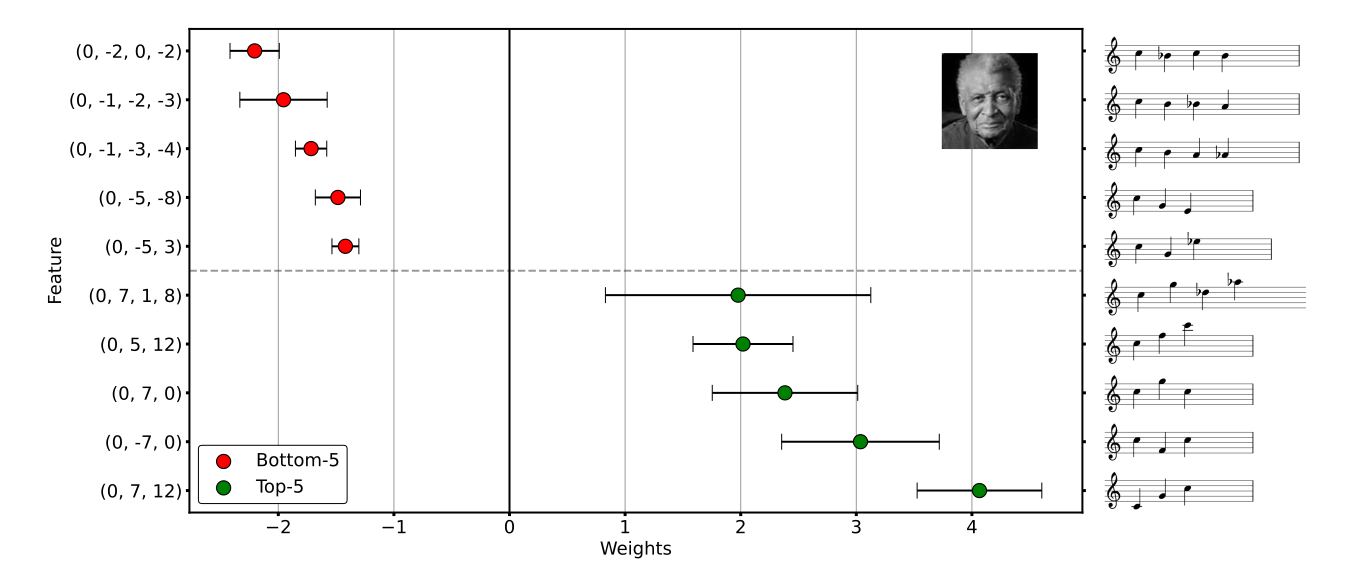
\includegraphics[width=1\textwidth]{figures/rsi_xai/figure_s4.pdf}
  \caption[Predictive melody features, Abdullah Ibrahim.]{Predictive melody features, Abdullah Ibrahim. This figure (and those following) shows standardised odds ratios obtained for every performer, following Figure \ref{fig:rsi_predictive_melody_features} in the full paper.}
\label{fig:rsi_sm_ibrahim_melody}
\end{figure}

\begin{figure}[!ht]
  \centering
  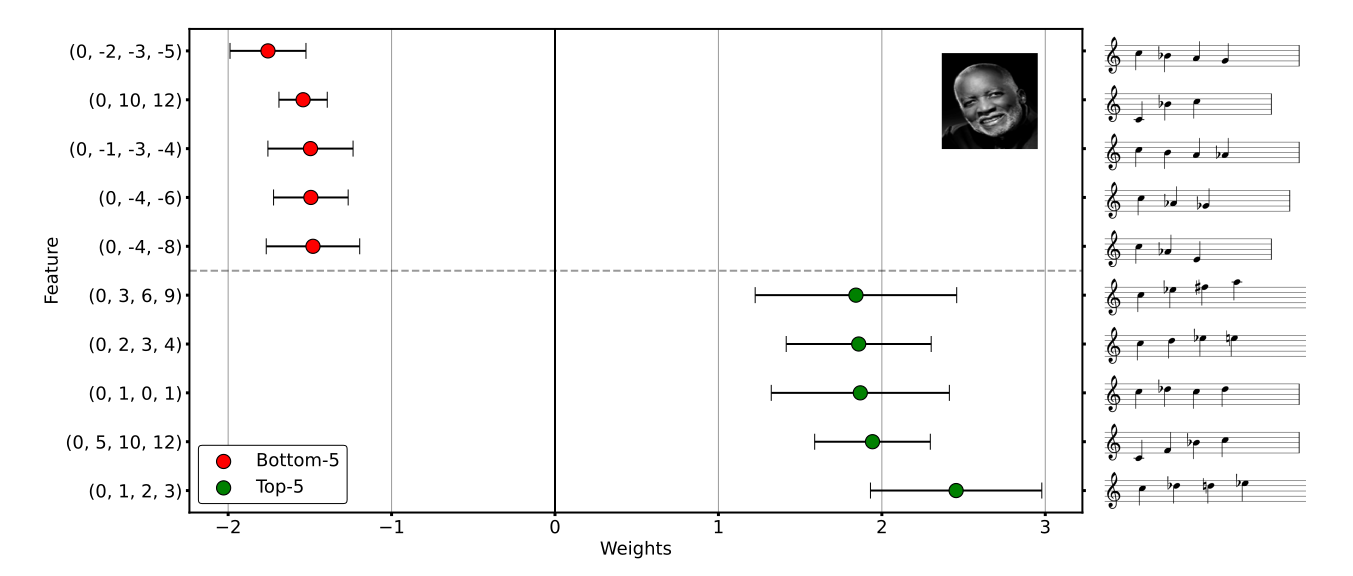
\includegraphics[width=1\textwidth]{figures/rsi_xai/figure_s5.pdf}
  \caption{Predictive melody features, Ahmad Jamal.}
\label{fig:rsi_sm_jamal_melody}
\end{figure}

\begin{figure}[!ht]
  \centering
  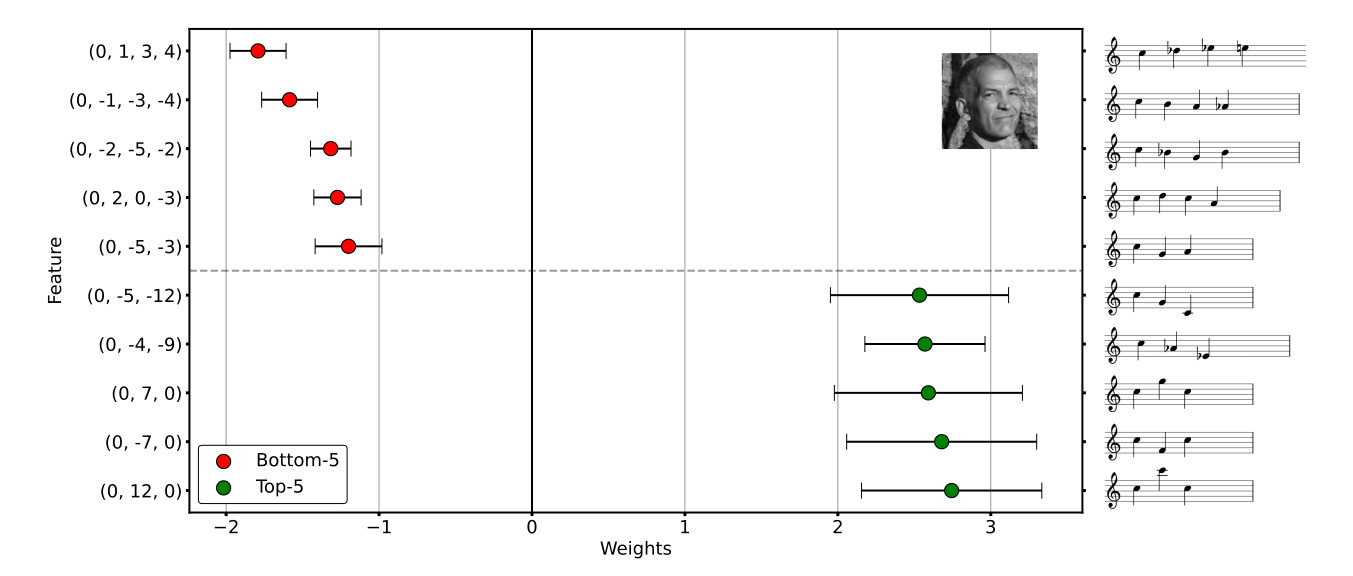
\includegraphics[width=1\textwidth]{figures/rsi_xai/figure_s6.pdf}
  \caption{Predictive melody features, Brad Mehldau.}
\label{fig:rsi_sm_mehldau_melody}
\end{figure}

\begin{figure}[!ht]
  \centering
  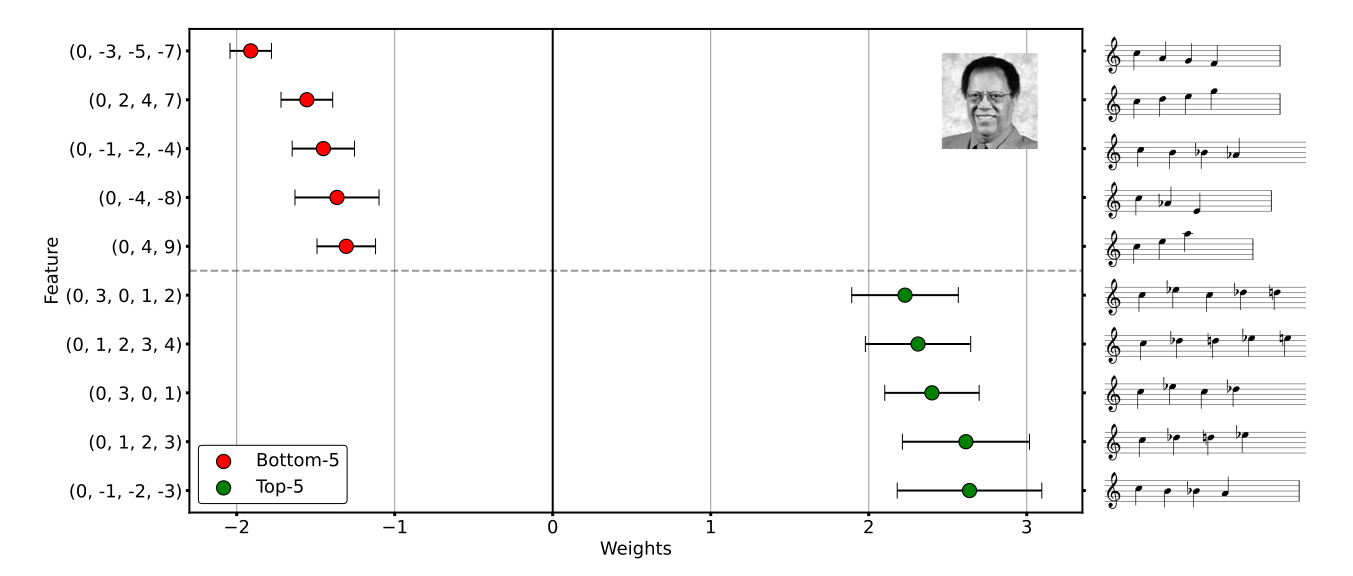
\includegraphics[width=1\textwidth]{figures/rsi_xai/figure_s7.pdf}
  \caption{Predictive melody features, Cedar Walton.}
\label{fig:rsi_sm_walton_melody}
\end{figure}

\begin{figure}[!ht]
  \centering
  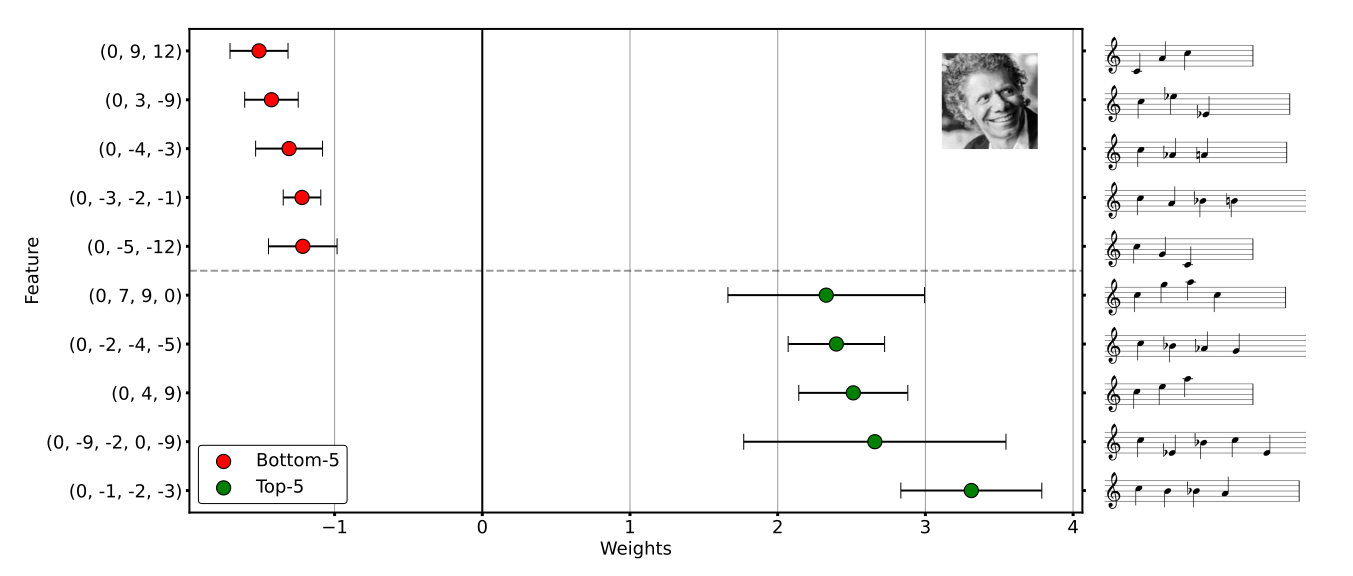
\includegraphics[width=1\textwidth]{figures/rsi_xai/figure_s8.pdf}
  \caption{Predictive melody features, Chick Corea.}
\label{fig:rsi_sm_corea_melody}
\end{figure}

\begin{figure}[!ht]
  \centering
  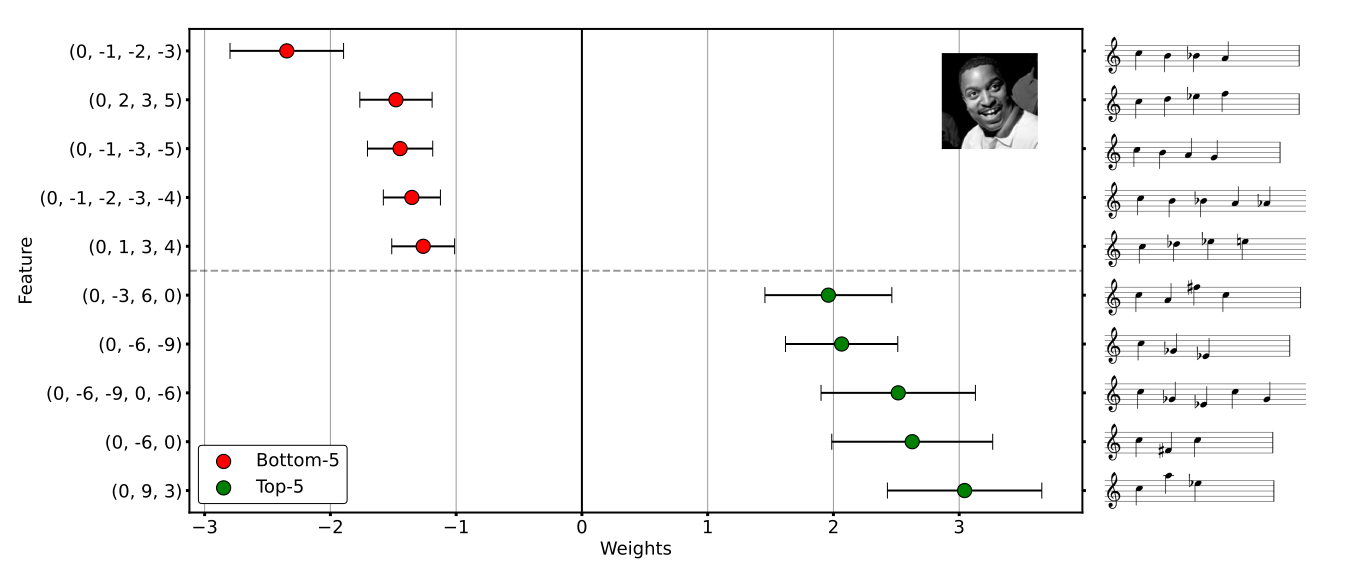
\includegraphics[width=1\textwidth]{figures/rsi_xai/figure_s9.pdf}
  \caption{Predictive melody features, Gene Harris.}
\label{fig:rsi_sm_harris_melody}
\end{figure}

\begin{figure}[!ht]
  \centering
  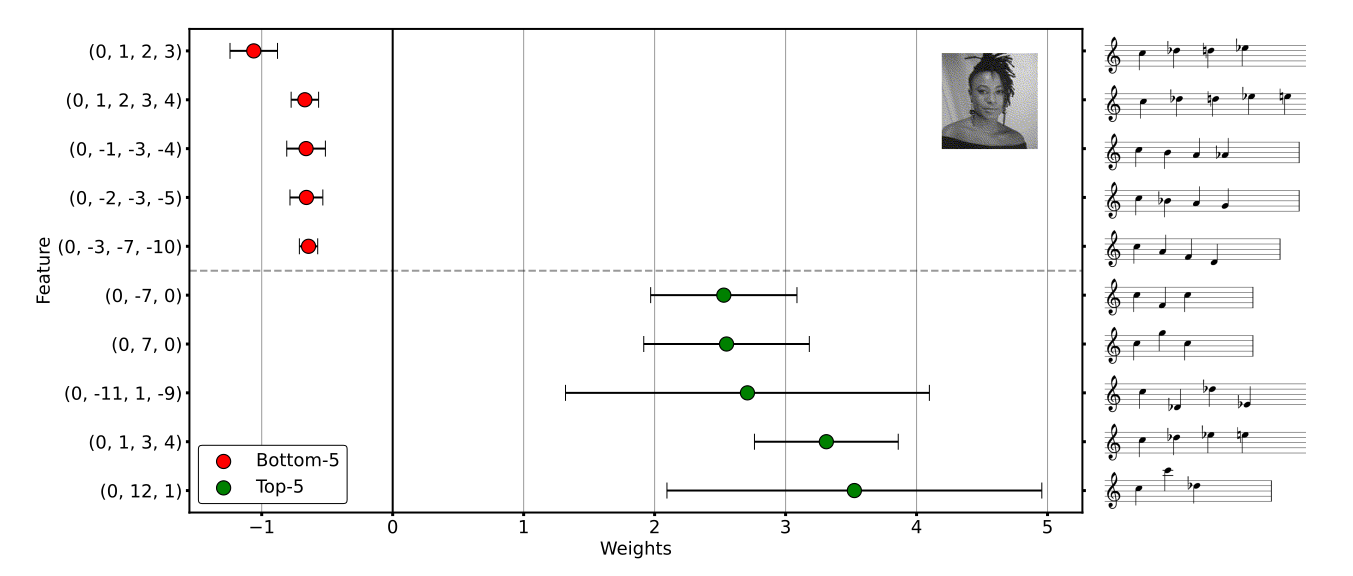
\includegraphics[width=1\textwidth]{figures/rsi_xai/figure_s10.pdf}
  \caption{Predictive melody features, Geri Allen.}
\label{fig:rsi_sm_allen_melody}
\end{figure}

\begin{figure}[!ht]
  \centering
  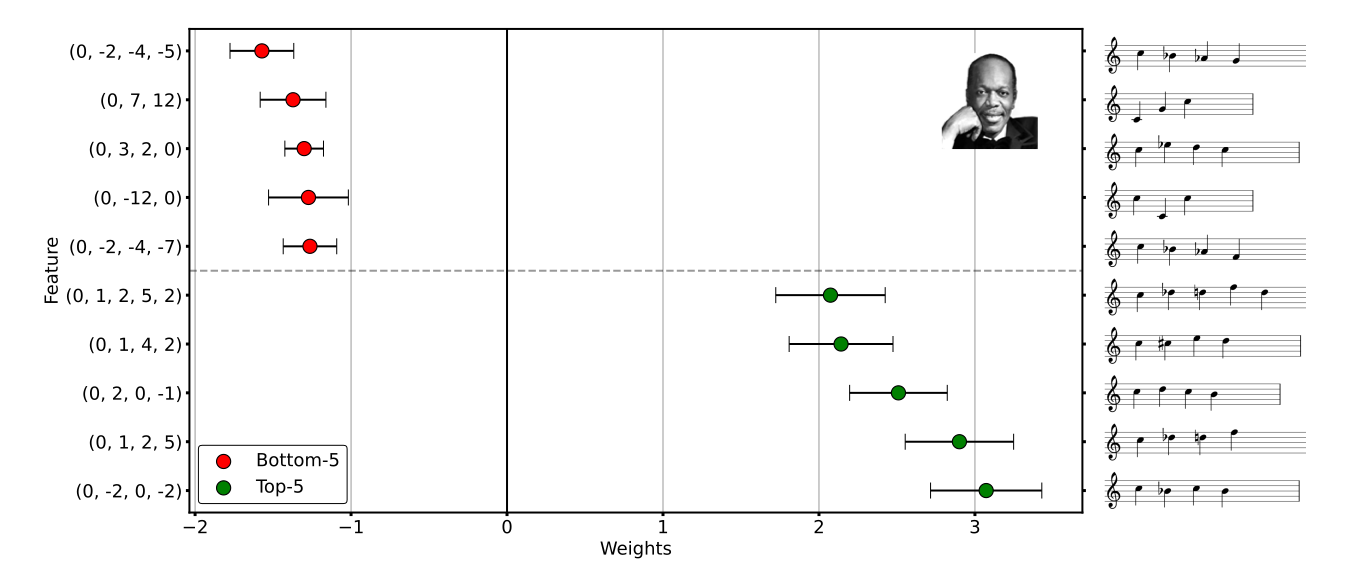
\includegraphics[width=1\textwidth]{figures/rsi_xai/figure_s11.pdf}
  \caption{Predictive melody features, Hank Jones.}
\label{fig:rsi_sm_jones_melody}
\end{figure}

\begin{figure}[!ht]
  \centering
  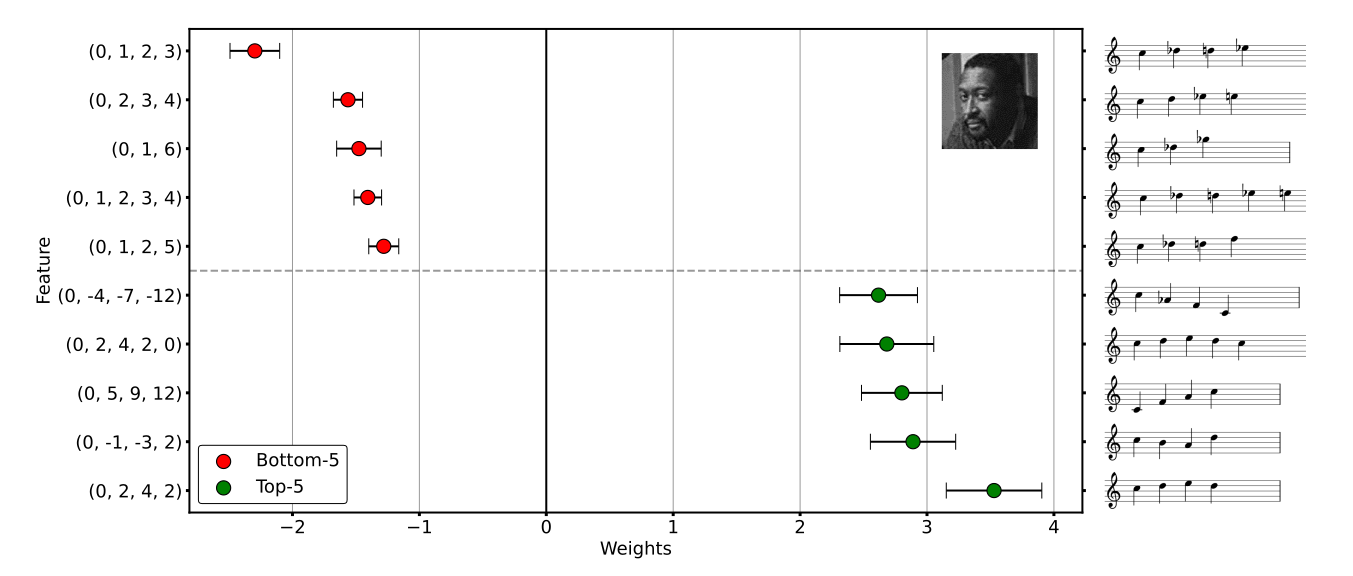
\includegraphics[width=1\textwidth]{figures/rsi_xai/figure_s12.pdf}
  \caption{Predictive melody features, John Hicks.}
\label{fig:rsi_sm_hicks_melody}
\end{figure}

\begin{figure}[!ht]
  \centering
  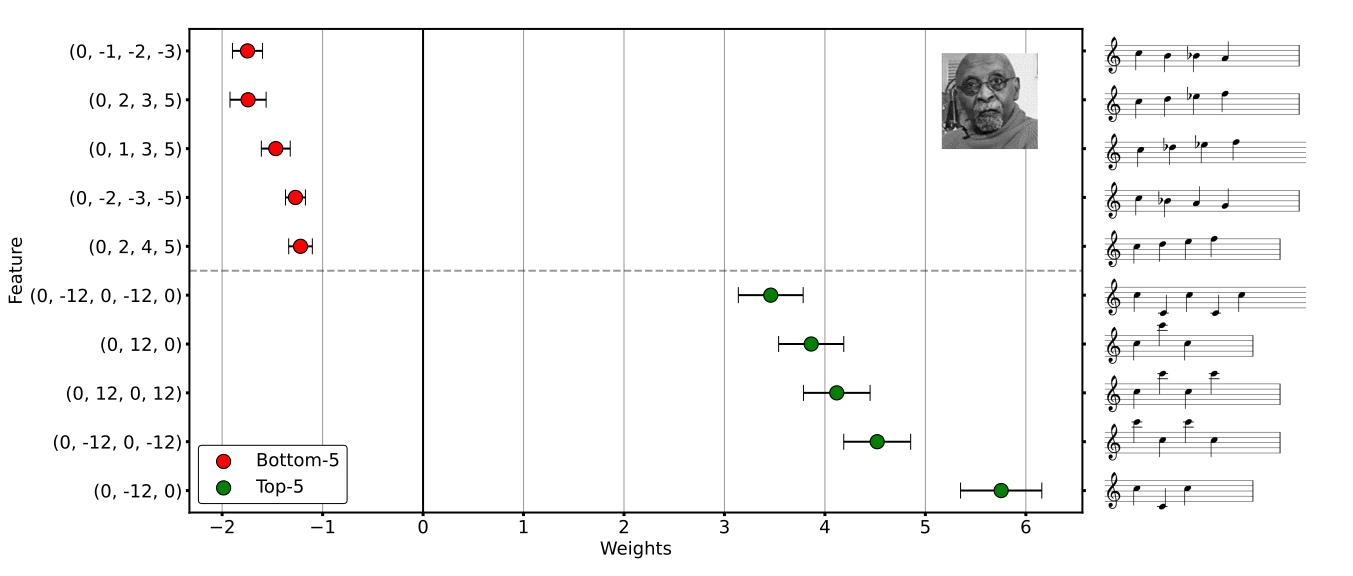
\includegraphics[width=1\textwidth]{figures/rsi_xai/figure_s13.pdf}
  \caption{Predictive melody features, Junior Mance.}
\label{fig:rsi_sm_mance_melody}
\end{figure}

\begin{figure}[!ht]
  \centering
  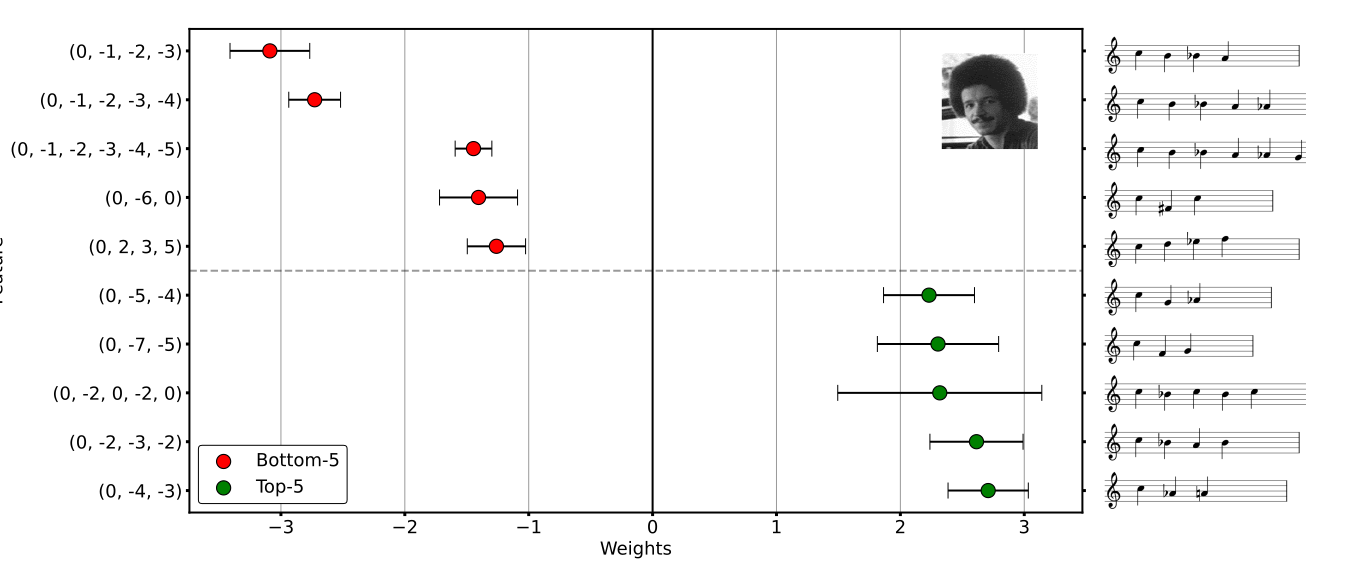
\includegraphics[width=1\textwidth]{figures/rsi_xai/figure_s14.pdf}
  \caption{Predictive melody features, Keith Jarrett.}
\label{fig:rsi_sm_jarrett_melody}
\end{figure}

\begin{figure}[!ht]
  \centering
  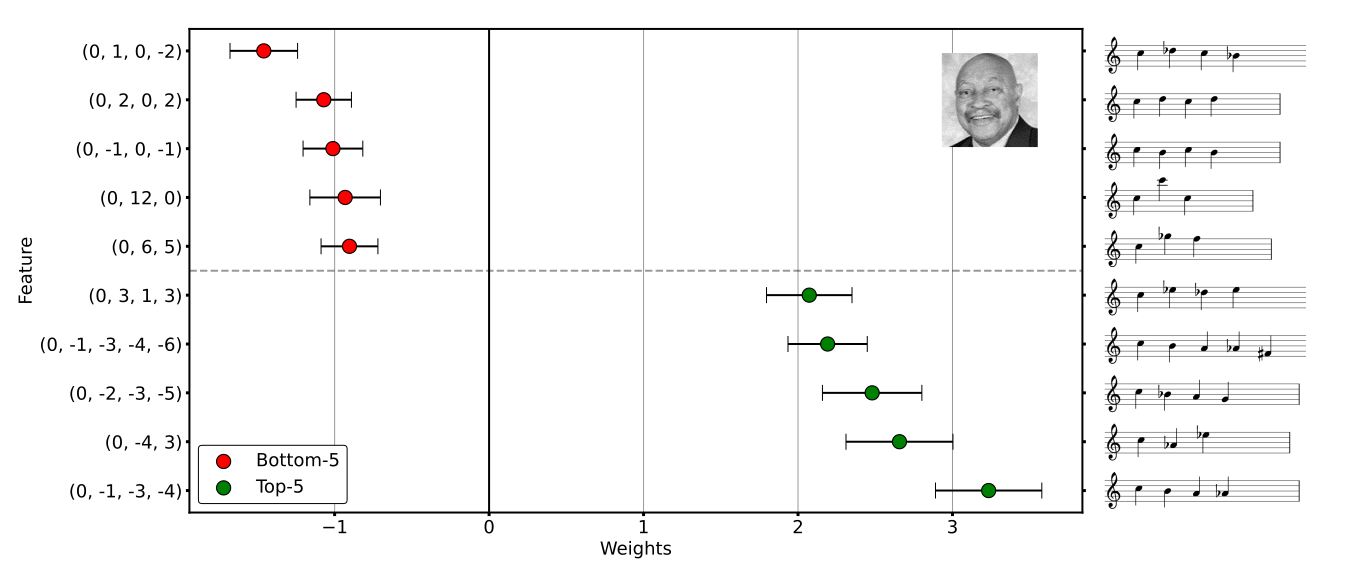
\includegraphics[width=1\textwidth]{figures/rsi_xai/figure_s15.pdf}
  \caption{Predictive melody features, Kenny Barron.}
\label{fig:rsi_sm_barron_melody}
\end{figure}

\begin{figure}[!ht]
  \centering
  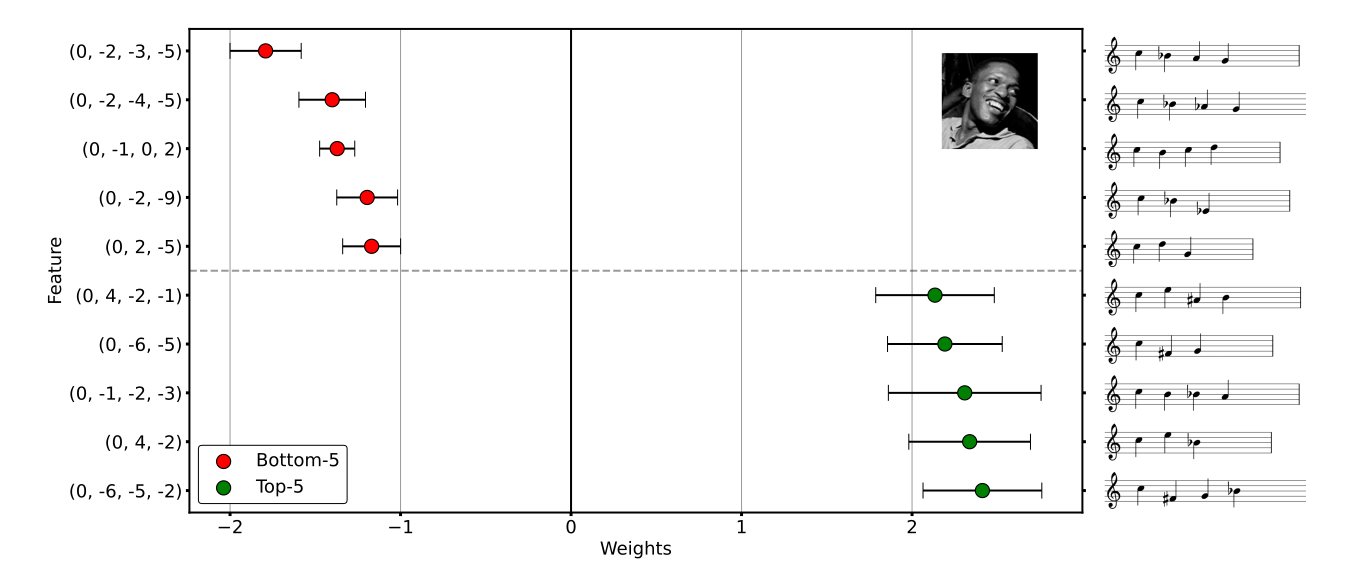
\includegraphics[width=1\textwidth]{figures/rsi_xai/figure_s16.pdf}
  \caption{Predictive melody features, Kenny Drew.}
\label{fig:rsi_sm_drew_melody}
\end{figure}

\begin{figure}[!ht]
  \centering
  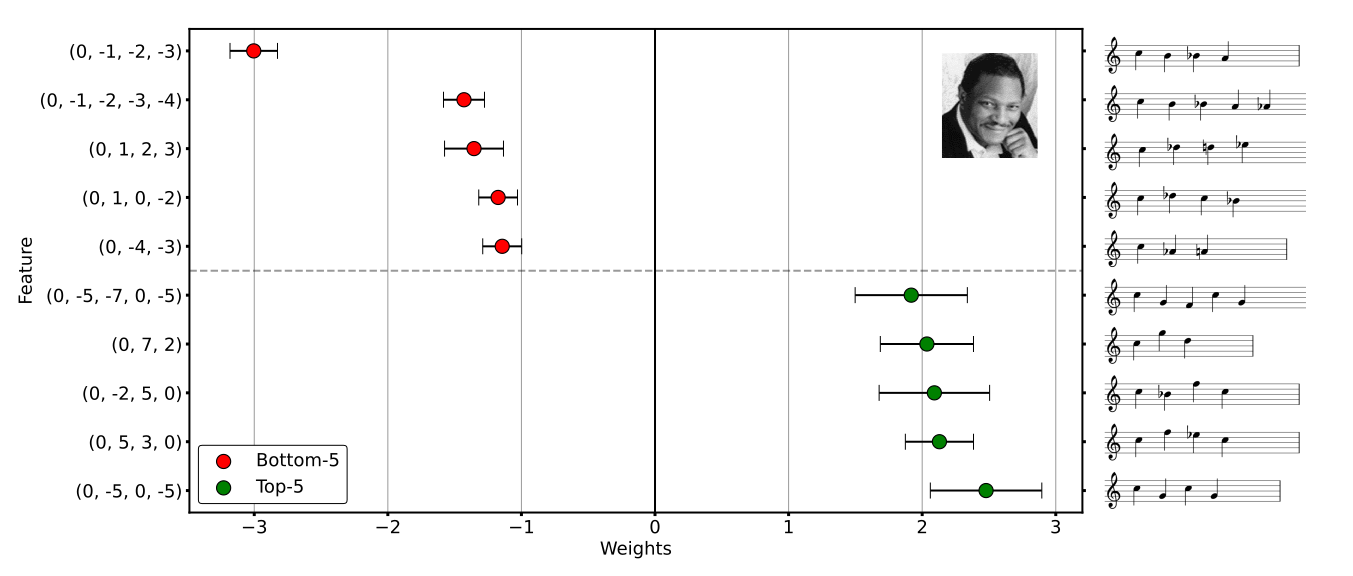
\includegraphics[width=1\textwidth]{figures/rsi_xai/figure_s17.pdf}
  \caption{Predictive melody features, McCoy Tyner.}
\label{fig:rsi_sm_tyner_melody}
\end{figure}

\begin{figure}[!ht]
  \centering
  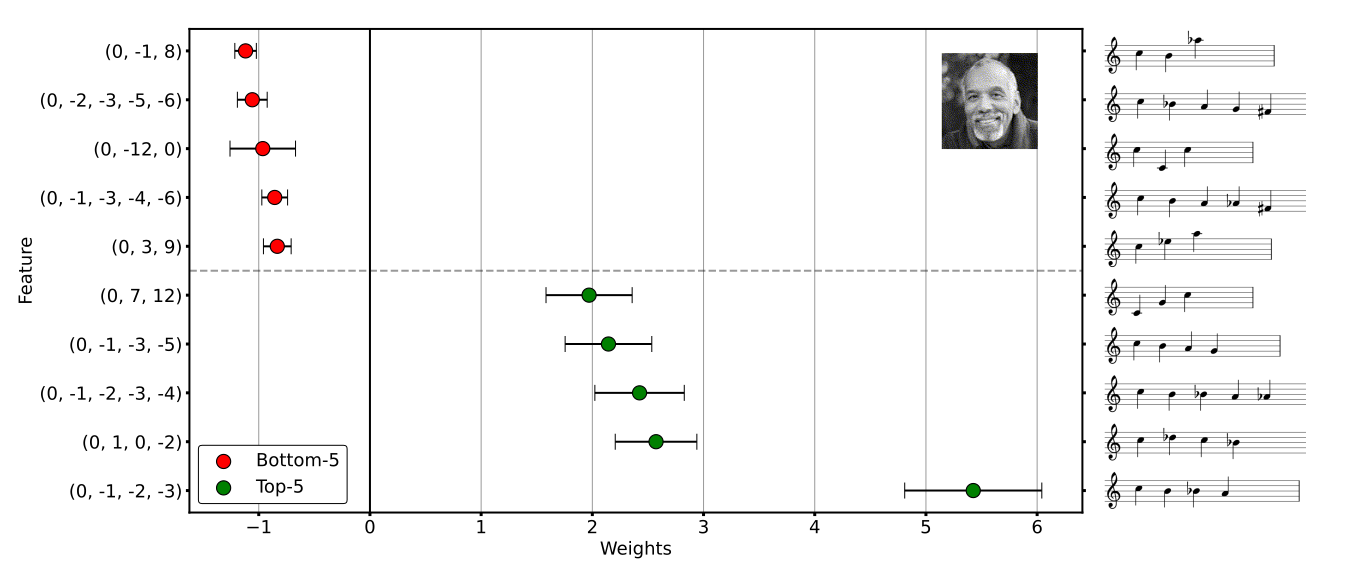
\includegraphics[width=1\textwidth]{figures/rsi_xai/figure_s18.pdf}
  \caption{Predictive melody features, Stanley Cowell.}
\label{fig:rsi_sm_cowell_melody}
\end{figure}

\begin{figure}[!ht]
  \centering
  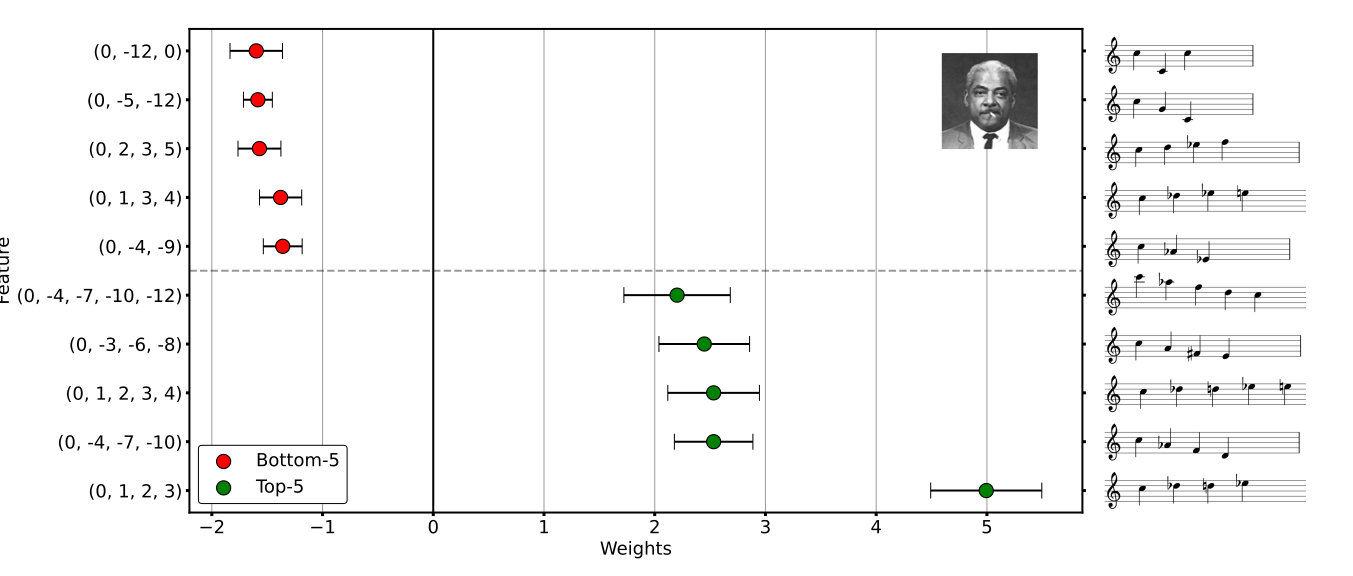
\includegraphics[width=1\textwidth]{figures/rsi_xai/figure_s19.pdf}
  \caption{Predictive melody features, Teddy Wilson.}
\label{fig:rsi_sm_wilson_melody}
\end{figure}

\begin{figure}[!ht]
  \centering
  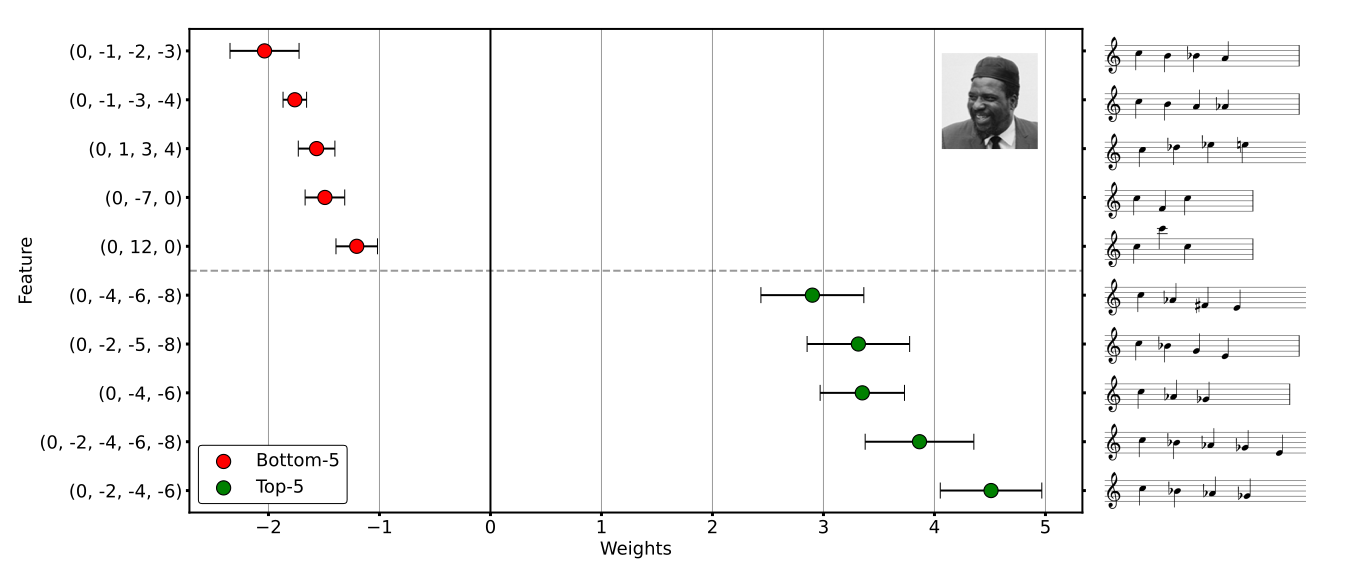
\includegraphics[width=1\textwidth]{figures/rsi_xai/figure_s20.pdf}
  \caption{Predictive melody features, Thelonious Monk.}
\label{fig:rsi_sm_monk_melody}
\end{figure}

\begin{figure}[!ht]
  \centering
  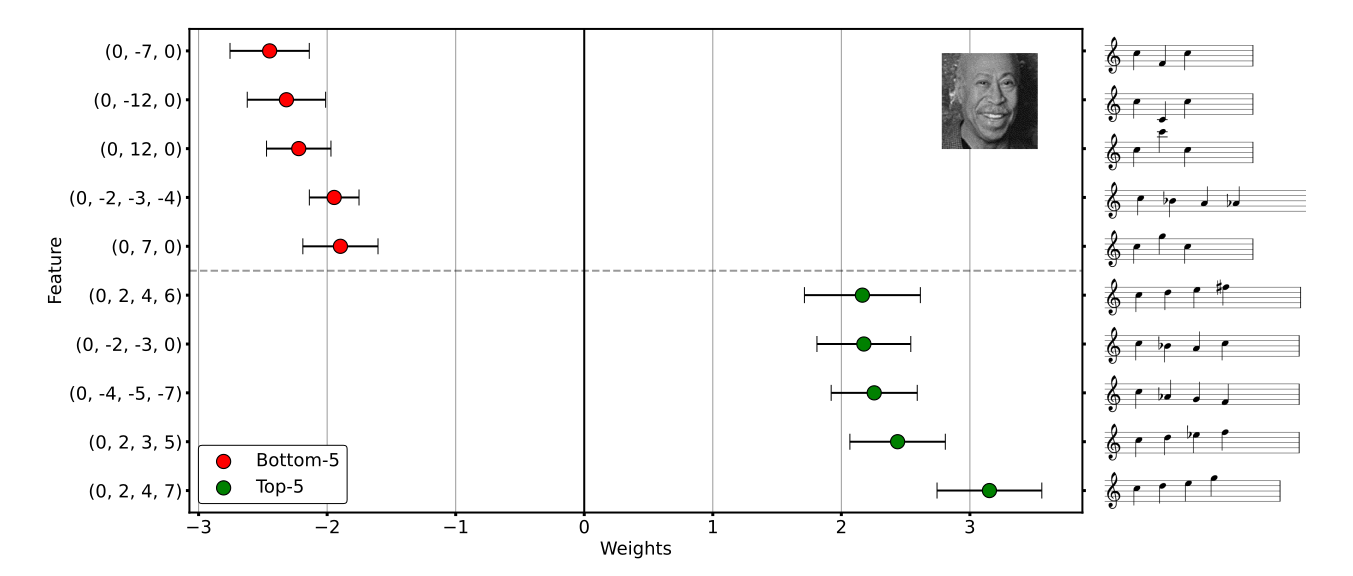
\includegraphics[width=1\textwidth]{figures/rsi_xai/figure_s21.pdf}
  \caption{Predictive melody features, Tommy Flanagan.}
\label{fig:rsi_sm_flanagan_melody}
\end{figure}

\begin{figure}[!ht]
  \centering
  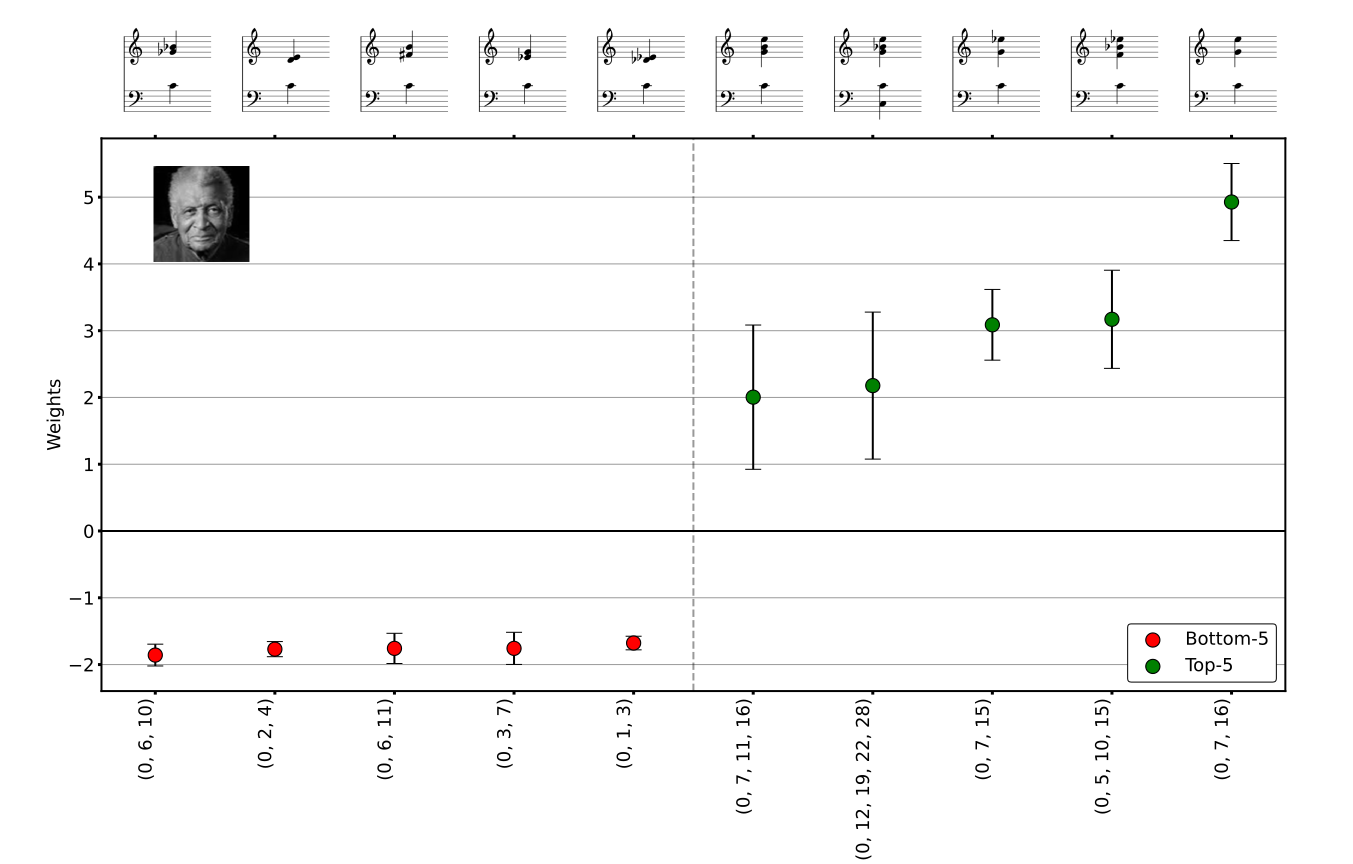
\includegraphics[width=1\textwidth]{figures/rsi_xai/figure_s22.pdf}
  \caption[Predictive harmony features, Abdullah Ibrahim.]{Predictive harmony features, Abdullah Ibrahim. Note that the direction of the axis in these figures is reversed compared to the previous figures, in order to accommodate the ``grand staff'' notation.}
\label{fig:rsi_sm_ibrahim_harmony}
\end{figure}

\begin{figure}[!ht]
  \centering
  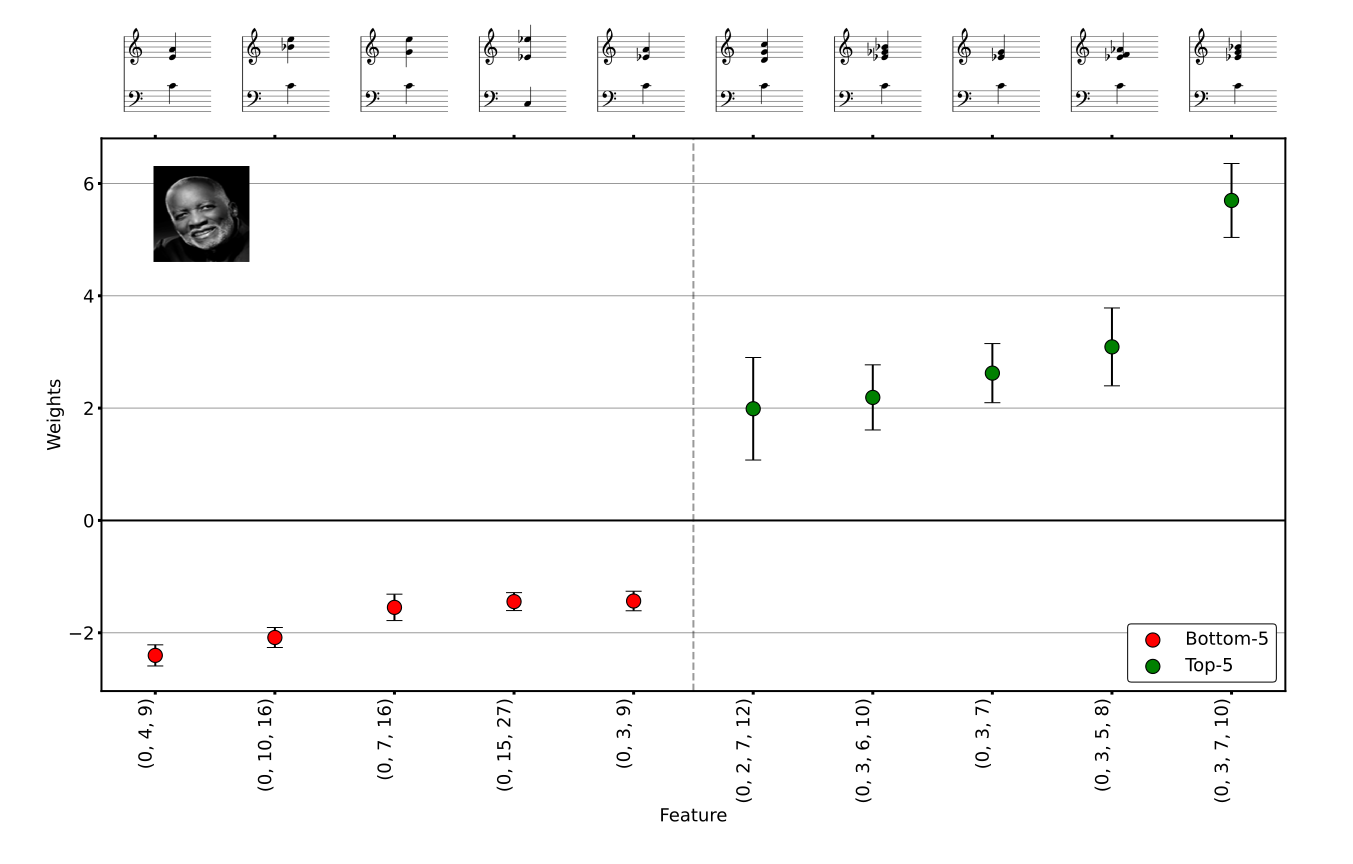
\includegraphics[width=1\textwidth]{figures/rsi_xai/figure_s23.pdf}
  \caption{Predictive harmony features, Ahmad Jamal.}
\label{fig:rsi_sm_jamal_harmony}
\end{figure}

\begin{figure}[!ht]
  \centering
  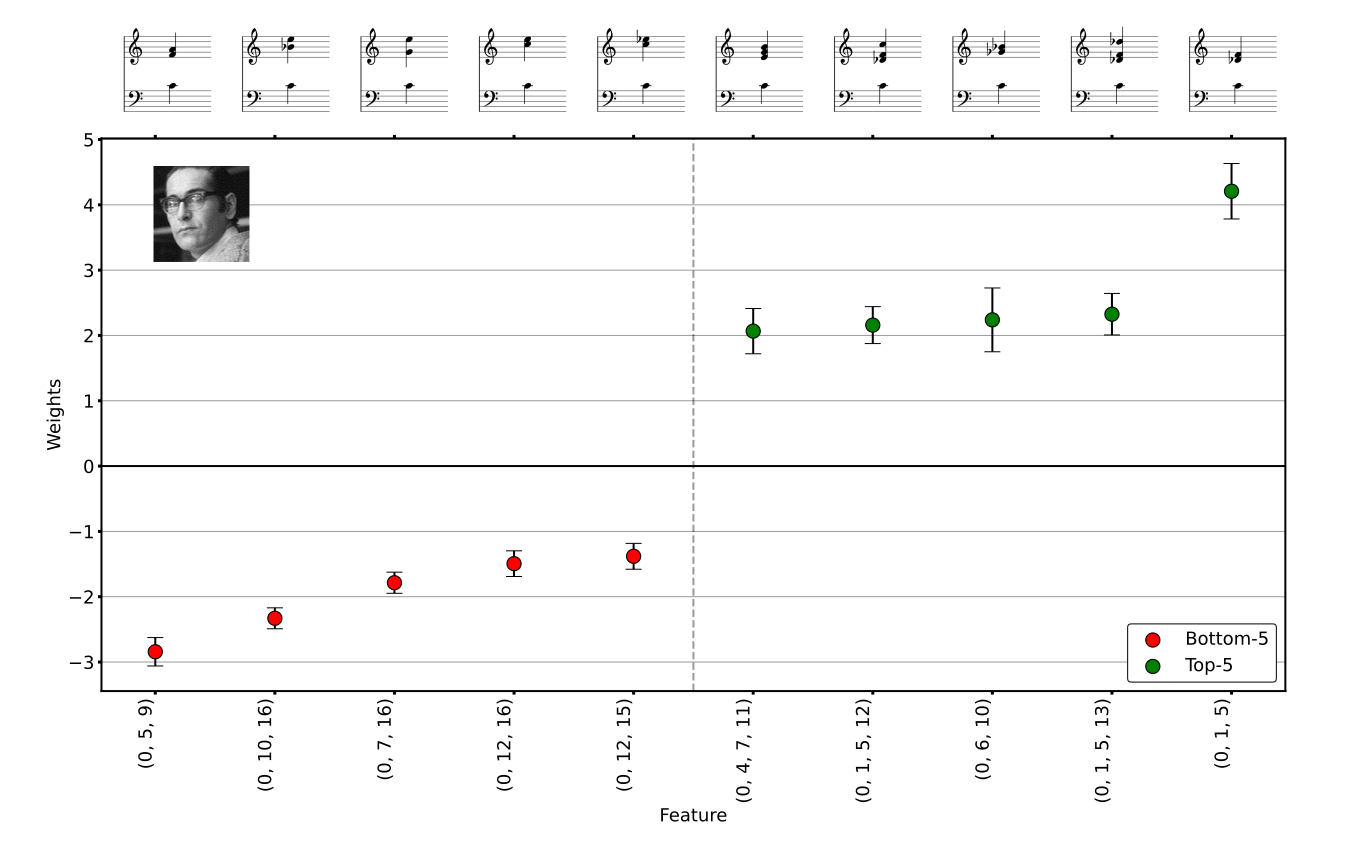
\includegraphics[width=1\textwidth]{figures/rsi_xai/figure_s24.pdf}
  \caption{Predictive harmony features, Bill Evans.}
\label{fig:rsi_sm_evans_harmony}
\end{figure}

\begin{figure}[!ht]
  \centering
  \includegraphics[width=1\textwidth]{figures/rsi_xai/figure_s25.pdf}
  \caption{Predictive harmony features, Brad Mehldau.}
\label{fig:rsi_sm_mehldau_harmony}
\end{figure}

\begin{figure}[!ht]
  \centering
  \includegraphics[width=1\textwidth]{figures/rsi_xai/figure_s26.pdf}
  \caption{Predictive harmony features, Cedar Walton.}
\label{fig:rsi_sm_walton_harmony}
\end{figure}

\begin{figure}[!ht]
  \centering
  \includegraphics[width=1\textwidth]{figures/rsi_xai/figure_s27.pdf}
  \caption{Predictive harmony features, Chick Corea.}
\label{fig:rsi_sm_corea_harmony}
\end{figure}

\begin{figure}[!ht]
  \centering
  \includegraphics[width=1\textwidth]{figures/rsi_xai/figure_s28.pdf}
  \caption{Predictive harmony features, Gene Harris.}
\label{fig:rsi_sm_harris_harmony}
\end{figure}

\begin{figure}[!ht]
  \centering
  \includegraphics[width=1\textwidth]{figures/rsi_xai/figure_s29.pdf}
  \caption{Predictive harmony features, Geri Allen.}
\label{fig:rsi_sm_allen_harmony}
\end{figure}

\begin{figure}[!ht]
  \centering
  \includegraphics[width=1\textwidth]{figures/rsi_xai/figure_s30.pdf}
  \caption{Predictive harmony features, Hank Jones.}
\label{fig:rsi_sm_jones_harmony}
\end{figure}

\begin{figure}[!ht]
  \centering
  \includegraphics[width=1\textwidth]{figures/rsi_xai/figure_s31.pdf}
  \caption{Predictive harmony features, John Hicks.}
\label{fig:rsi_sm_hicks_harmony}
\end{figure}

\begin{figure}[!ht]
  \centering
  \includegraphics[width=1\textwidth]{figures/rsi_xai/figure_s32.pdf}
  \caption{Predictive harmony features, Junior Mance.}
\label{fig:rsi_sm_mance_harmony}
\end{figure}

\begin{figure}[!ht]
  \centering
  \includegraphics[width=1\textwidth]{figures/rsi_xai/figure_s33.pdf}
  \caption{Predictive harmony features, Keith Jarrett.}
\label{fig:rsi_sm_jarrett_harmony}
\end{figure}

\begin{figure}[!ht]
  \centering
  \includegraphics[width=1\textwidth]{figures/rsi_xai/figure_s34.pdf}
  \caption{Predictive harmony features, Kenny Barron.}
\label{fig:rsi_sm_barron_harmony}
\end{figure}

\begin{figure}[!ht]
  \centering
  \includegraphics[width=1\textwidth]{figures/rsi_xai/figure_s35.pdf}
  \caption{Predictive harmony features, Kenny Drew.}
\label{fig:rsi_sm_drew_harmony}
\end{figure}

\begin{figure}[!ht]
  \centering
  \includegraphics[width=1\textwidth]{figures/rsi_xai/figure_s36.pdf}
  \caption{Predictive harmony features, McCoy Tyner.}
\label{fig:rsi_sm_tyner_harmony}
\end{figure}

\begin{figure}[!ht]
  \centering
  \includegraphics[width=1\textwidth]{figures/rsi_xai/figure_s37.pdf}
  \caption{Predictive harmony features, Oscar Peterson.}
\label{fig:rsi_sm_peterson_harmony}
\end{figure}

\begin{figure}[!ht]
  \centering
  \includegraphics[width=1\textwidth]{figures/rsi_xai/figure_s38.pdf}
  \caption{Predictive harmony features, Stanley Cowell.}
\label{fig:rsi_sm_cowell_harmony}
\end{figure}

\begin{figure}[!ht]
  \centering
  \includegraphics[width=1\textwidth]{figures/rsi_xai/figure_s39.pdf}
  \caption{Predictive harmony features, Teddy Wilson.}
\label{fig:rsi_sm_wilson_harmony}
\end{figure}

\begin{figure}[!ht]
  \centering
  \includegraphics[width=1\textwidth]{figures/rsi_xai/figure_s40.pdf}
  \caption{Predictive harmony features, Thelonious Monk.}
\label{fig:rsi_sm_monk_harmony}
\end{figure}

\begin{figure}[!ht]
  \centering
  \includegraphics[width=1\textwidth]{figures/rsi_xai/figure_s41.pdf}
  \caption{Predictive harmony features, Tommy Flanagan.}
\label{fig:rsi_sm_flanagan_harmony}
\end{figure}

\begin{figure}[!ht]
  \centering
  \includegraphics[width=1\textwidth]{figures/rsi_xai/figure_s42.pdf}
  \caption[Further masked piano rolls generated with \GLS{LIME}.]{Further masked piano rolls generated with \GLS{LIME}. Each panel shows a single 30-second clip from a transcription of a performance by (a) Abdullah Ibrahim, (b) Chick Corea, and (c) Keith Jarrett, taken from the held-out test split. Highlighted in blue are the top five areas of the piano roll that positively contribute to predicting the target label according to \GLS{LIME}.}
\label{fig:rsi_sm_lime_plots}
\end{figure}

\chapter{Harmonic Concepts}\label{chap:rsi_haerle_concepts}

The following table describes the twenty harmonic concepts taken from \citep{Haerle1994} that are used in Section~\ref{sec:rsi_factorised_cavs}.\clearpage

\begin{sidewaystable}[ht]
    \centering
    \caption[Descriptions of the twenty chapters in \citet{Haerle1994} that make up the concept dataset.]{Descriptions of the twenty chapters in \citet{Haerle1994} that make up the concept dataset. The text is adapted and summarised from the didactic descriptions that precede each chapter.}
    \label{tab:rsi_sm_haerle_concepts}
    \begin{tabular}{lcp{15cm}}
        \toprule
         \textbf{Name} 
&\textbf{Number} & \textbf{Description} \\
        \midrule
         Block Chords 
&1 & Includes ``block''-type, closed chords that are built on stacked thirds and outline common voicings for major, dominant, and minor, and diminished sevenths, as well as the same chords with suspended fourths. \\
         Shell Voicings 
&2 & Includes ``shell''-type, open chord voicings that outline extensions beyond the seventh (e.g., sixths, ninths, flattened fifths). \\
         Diatonic 7th Chords 
&3 & Includes diatonic seventh chords walked sequentially through major and minor tonalities. \\
         Cycle Progressions 
&4 & Connects different inversions of voicings in an idiomatic way as part of typical progressions. Common progressions represented in this concept are I-IV in major and minor, dominant 7th cycles, I-V in major and V-I in major and minor. \\
         II-V-I's in Major and Minor 
&5 & A logical extension of the Cycle Progressions concept which moves on to playing complete II-V-I cadences in major and minor keys. \\
         I-IV Cycle Progression 
&6 & A common cycle progression which moves from the key centre to the IV chord which, in turn, becomes a new key centre. \\
         Modal Fourthy Voicings 
&7 & Fourthy voicings which are moved through a Dorian mode. \\
         ``So What'' Voicings 
&8 & A particular fourthy structure probably best known from its use in the Miles Davis composition ``So What''. Presented in both minor (Dorian) and major (Lydian) modes. \\
         Modal ``So What'' Voicings 
&9 & Fourthy voicings which are moved through a Dorian mode. The ``So What'' voicing is used and, rather than keeping its pure structure, it changes slightly as it is moved through the Dorian scale. \\
         Fourthy II-V-I's 
&10 & II-V-I progressions using the ``So What'' voicing. The structure is built on the root of the II chord and on the 3rd of the I chord. Since the voicing doesn't clearly fit or imply a dominant chord, the V chord simply involves chromatin side-slipping up or down to the I chord. \\
    \end{tabular}
\end{sidewaystable}

\begin{sidewaystable}[ht]
    \centering
    \begin{tabular}{lcp{15cm}}
             Tri-Tone Sub II-V-I's 
&11 & II-V-I progressions using both the normal II and V chords and the II-V located a tri-tone away. The result is a deception as though the cadence was suddenly modulating to a distant key. \\
         Polychordal II-V-I's 
&12 & II-V-I progressions involving polychordal structures in which the left hand plays a conventional inversion and the right hand plays some kind of triadic structure to create extensions and/or alterations of the harmony. \\
         Cycling Altered Dominants 
&13 & Progressions involving polychordal structures in which the left hand plays a dominant structure and the right hand plays some kind of triadic structure to create extensions and/or alterations of the harmony. \\
         Polychordal Blues Voicings 
&14 & Twelve-bar blues progressions involving polychordal structures in which the left hand plays a conventional inversion and the right hand plays some kind of triadic structure to fill out a two-hand voicing of the harmony. \\
         Fourthy Blues Voicings 
&15 & Blues progressions involving fourthy structures in which the left hand plays a conventional inversion and the right hand plays a structure of two perfect fourths to fill out a two-hand voicing of the harmony. \\
         Major 7th Blues Voicings 
&16 & Blues progressions incorporating voicings from other concepts, including II-V-I's in Major and Minor (concept 5), I-IV Cycle Progression (6), and Tri-Tone Sub II-V-I's (11). \\
         Minor Blues Voicings 
&17 & Minor blues progressions involving fourthy structures in which the left hand plays a conventional inversion and the right hand plays a structure of two perfect fourths to fill out a two-hand voicing of the harmony. \\
         Dominant 7th Polychords 
&18 & Dominant seventh chords where the left hand plays a conventional inversion and the right hand plays some additional construction (e.g., involving flattening and sharpening of the fifth and ninth scale degrees). \\
         Dominant Polychord Groups 
&19 & Utilizes five of the polychord formulas from the previous concept (Dominant 7th Polychords) in groups with each other against a conventional inversion in the left hand to create melodic motion. \\
         Diminished Substitutions &20 & Utilizes voicings that are derived from the half-whole diminished scale that relates to a dominant seventh chord. Since the same scale relates to four different dominant seventh chords, it makes this device possible. \\
        \bottomrule
    \end{tabular}
\end{sidewaystable}
\chapter{Musician Self-Reports}\label{chap:mp_appendix}

The following tables contain the free text responses given by participants in the online surveys completed following each condition in the experiment, as described in Section~\ref{sec:mp_experimental_procedure}. Not all participants chose to provide free text responses, and some performers only commented on a small number of conditions.

Responses have been edited to ensure the anonymity of participants, such that direct references to participant’s names have been replaced by generic statements corresponding to their instrument, instead (e.g., ‘the drummer’, ‘the pianist’ etc.). No other editorial changes have been made and the spelling and grammar of the original responses (which were entered by participants on mobile phones, tablets, and laptops) have been maintained. 

Note finally that, as participants were not informed about the addition of latency and jitter to their partner’s performance, their comments occasionally reflect a naive understanding of the procedure and thus may be misleading in light of the full methodological description found in Section~\ref{sec:mp_methods}. For instance, one participant misconstrued the change in tempo of their performance as the result of their partner hearing a metronome playing at a slower tempo through their headphones.\clearpage

\begin{sidewaystable}[]
\centering
\caption{Latency: 0 ms, Jitter: 0 ms}
\begin{tabular}{l c c p{15cm}}
\toprule
\textbf{Instrument} & \textbf{Duo} & \textbf{Session} & \textbf{Comment} \\ \midrule
Piano & 1 & 1 & Possibly just warming up, but it felt very easy to interact with my partner and respond to our behaviours \\ 
Piano & 1 & 2 & Smooth, responded to little rhythmic cues and things, felt natural \\ 
Drums & 3 & 1 & I could hear [the pianist] well and it we came up with some nice interactive phrases (call and response, repetition, accents played together) \\ 
Piano & 3 & 1 & Most successful yet - tempo was solid from the start and both played with more precision and clarity. Interaction was good \\ 
Drums & 3 & 2 & It was easy to communicate and we had some nice call and response going, my comping was a bit sloppy which was throwing me off a bit \\ 
Piano & 3 & 2 & Pretty solid tempo, some more interaction this time \\ 
Piano & 4 & 1 & Felt slightly more difficult to coordinate, and to be creative - perhaps purely a natural dip though. \\ 
Piano & 4 & 2 & Didn't seem to be any/much feed disruption. As such, very creative and interactive performance. \\ \bottomrule
\end{tabular}
\end{sidewaystable}\clearpage

\begin{sidewaystable}[]
\centering
\caption{Latency: 23 ms, Jitter: 0 ms}
\begin{tabular}{l c c p{15cm}}
\toprule
\textbf{Instrument} & \textbf{Duo} & \textbf{Session} & \textbf{Comment} \\ \midrule
Drums & 1 & 1 & Sounds better when we slow down to meet each other even when we're not in sync yet. I don't know why! Fills do not make anything easier for anyone which is a shame because they are fun to play \\ 
Piano & 1 & 1 & We were just on totally different wavelengths. I ended up ignoring [the drummer] totally, both audio and visual, just to see if he could catch on, but it didn’t make it easier \\ 
Drums & 1 & 2 & They feel like they're getting easier but that requires less concentration and interactions \\ 
Piano & 1 & 2 & This one felt good - I even forgot my brief and got a bit out of hand melodically \\ 
Drums & 3 & 1 & It was much easier to hold the tempo and the difference in quality of the visual did not matter as we could follow each other’s playing effectively. I felt relieved to be able to interact much more easily, it felt like we were really playing together \\ 
Piano & 3 & 1 & We were playing in the same tempo this time - more dynamic variation and interaction than before \\ 
Piano & 3 & 2 & Started out a bit hesitant but interaction improved as we went on \\ 
Piano & 4 & 1 & It felt even more difficult to synchronise our beat. It seemed that [the drummer] was setting a slightly slower tempo than mine, which occasionally got slightly slower. This was difficult to 'sit into' the groove, and make creative ideas. \\ 
Piano & 4 & 2 & Good creative energy and flow, particularly in second half of Condition. \\ \bottomrule
\end{tabular}
\end{sidewaystable}\clearpage

\begin{sidewaystable}[]
\centering
\caption{Latency: 23 ms, Jitter: 0.5x}
\begin{tabular}{l c c p{15cm}}
\toprule
\textbf{Instrument} & \textbf{Duo} & \textbf{Session} & \textbf{Comment} \\ \midrule
Drums & 1 & 1 & Felt like a battle of wills. When I finally gave in and slowed, keys suddenly jumped ahead as if to mess with me! \\ 
Piano & 1 & 1 & We definitely slowed down again, but this time I figured out why because what I could see and hear seemed to all match up. We just couldn’t manage to communicate time properly somehow \\ 
Drums & 1 & 2 & We both played big heavy stuff and it seemed to help us sound (not necessarily be) in time \\ 
Piano & 1 & 2 & A good final one, thank you [NB. participant refers directly to author here]. We got beyond synchronicity and got onto shape and musicality \\ 
Drums & 2 & 2 & Felt like I dragged a bit. \\ 
Drums & 3 & 1 & It was easy to communicate but it didn’t feel 100\% fluid \\ 
Piano & 3 & 1 & Tempo felt relatively secure - not as much interaction \\ 
Drums & 3 & 2 & I could hear [the pianist] well and in time and felt like we played together. We could play intricate rhythms together confidently \\ 
Piano & 3 & 2 & Tried to push the tempo more with walking bass to avoid slowing down - felt quite draggy \\ 
Piano & 4 & 1 & Relatively simple again. \\ 
Piano & 4 & 2 & Pretty well synchronised, good groove. \\ \bottomrule
\end{tabular}
\end{sidewaystable}\clearpage

\begin{sidewaystable}[]
\centering
\caption{Latency: 23 ms, Jitter: 1.0x}
\begin{tabular}{l c c p{15cm}}
\toprule
\textbf{Instrument} & \textbf{Duo} & \textbf{Session} & \textbf{Comment} \\ \midrule
Drums & 1 & 1 & That felt harder than the warm up but that could be because now I know it's the real deal \\ 
Piano & 1 & 1 & The combination of seeing and hearing meant that we could shape the performance together \\ 
Piano & 1 & 2 & Again we felt connected and interactive \\ 
Drums & 3 & 1 & I felt like it wasn’t as smooth as before but couldn’t tell why, it seemed that we were mostly hearing each other in time \\ 
Piano & 3 & 1 & Unsure whether tempo dipped naturally here or not - felt like we slowed down after the click \\ 
Drums & 3 & 2 & It was mostly easy to communicate but there were a couple of moments where we got a bit out of time \\ 
Piano & 3 & 2 & Tempo seemed to start to deviate halfway through? \\ 
Piano & 4 & 1 & We were pretty good at adjusting to the sudden changes of tempo, having become accustomed to it over the last few Conditions. \\ 
Piano & 4 & 2 & Moments of ride cymbal 'jolting' were subsumed effectively within the groove. \\ 
Piano & 5 & 2 & Fluctuation in tempo \\ \bottomrule
\end{tabular}
\end{sidewaystable}\clearpage

\begin{sidewaystable}[]
\centering
\caption{Latency: 45 ms, Jitter: 0.0x}
\begin{tabular}{l c c p{15cm}}
\toprule
\textbf{Instrument} & \textbf{Duo} & \textbf{Session} & \textbf{Comment} \\ \midrule
Drums & 1 & 1 & Really frustrating, felt as if keys were dragging slightly so tried to continue at initial tempo. Never lined up so tried to join them. Inevitably slowed down more and more. Frustrating to not be able to use body language effectively \\ 
Piano & 1 & 1 & Interesting one, I thought we were communicating quite effectively but this time I was looking at the screen more and could see that [the drummer] was finding it much more difficult than me. He was trying to dictate a different tempo but it seemed okay to me! It threw me off a bit \\ 
Drums & 1 & 2 & We weren't that out of sync we just slowed down lots! At first this was frustrating - this is now almost guaranteed and very much expected \\ 
Piano & 1 & 2 & The rallentando effect was there but less prominently so \\ 
Drums & 3 & 1 & I felt like we dragged a bit and something was a little bit off but it was still possible to mostly play together \\ 
Piano & 3 & 1 & Some dip in tempo this time at the start - less pronounced than before. Adjusted to the ride cymbal mainly - some dynamic interaction \\ 
Drums & 3 & 2 & We didn’t have to look at each other much to understand what was going on. I think there was an awareness that something might be weird so there was a certain apprehension in sparser sections \\ 
Piano & 3 & 2 & Still felt like we slow down immediately - trying to push tempo. Some dynamic changes. \\ 
Piano & 4 & 1 & We hit a creative peak in the solo! The small disruptions of beats being lost/tempo increasing or decreasing helped with the energy of the solo. \\ \bottomrule
\end{tabular}
\end{sidewaystable}\clearpage

\begin{sidewaystable}[]
\centering
\caption{Latency: 45 ms, Jitter: 0.5x}
\begin{tabular}{l c c p{15cm}}
\toprule
\textbf{Instrument} & \textbf{Duo} & \textbf{Session} & \textbf{Comment} \\ \midrule
Drums & 1 & 1 & Slowed down but found a groove. Feels more interactive when it's harder to sync up - you can really just ignore each other and do your own thing at all \\ 
Piano & 1 & 1 & I didn’t notice us slowing down but did notice that we had slowed down \\ 
Drums & 1 & 2 & Eventually settled into a groove but felt like I was wrestling for tempo control \\ 
Piano & 1 & 2 & There were a few instances of asynchronicity but I think as a result of performer error rather than communication failure \\ 
Drums & 2 & 1 & I have a tendency to push ahead when others are so far behind, but otherwise liked the 'feel' of this (feeling behind the beat rather than in a different place). \\ 
Drums & 3 & 1 & I felt like the tempo was dragging a lot in inconsistent amounts and I was finding it difficult to predict when the next bass crotchet was coming in - this made it very difficult to hold the tempo and communicate in an effective way \\ 
Piano & 3 & 1 & Initially thought [the drummer] might have just started off a bit slow from the initial click - after a chorus it was clear he had a different tempo in his ears and I decided to go with his ride cymbal \\ 
Drums & 3 & 2 & It was mostly easy to communicate but I felt like I had to play ahead of [the pianist] some of the time \\ 
Piano & 3 & 2 & Slowed down at the beginning \\ 
Piano & 4 & 1 & The tempo feed from [the drummer] immediately got slower, and got increasingly slow throughout. Cadence points became increasingly difficult to execute convincingly. Jolts of lack of synchronised tempo made creativity difficult. \\ 
Piano & 4 & 2 & Similar, pretty good interaction. Pretty creative, nothing jaw-dropping. \\ 
Piano & 5 & 2 & Felt like [the drummer] was slowing down \\ \bottomrule
\end{tabular}
\end{sidewaystable}\clearpage

\begin{sidewaystable}[]
\centering
\caption{Latency: 45 ms, Jitter: 1.0x}
\begin{tabular}{l c c p{15cm}}
\toprule
\textbf{Instrument} & \textbf{Duo} & \textbf{Session} & \textbf{Comment} \\ \midrule
Drums & 1 & 1 & Plowing on at right tempo didn't really seem like an option, esp in a performance where cohesiveness probs more important than tempo accuracy. Slowed down a lot but made it quite a fun heavy groove when we got the hang of it \\ 
Piano & 1 & 1 & The experience felt similar to the previous one but throughout rather than coming and going. We slowed down dramatically and didn’t manage to recommunicate a new tempo \\ 
Drums & 1 & 2 & Actually remained fairly in tempo until later on where we slowed down. \\ 
Piano & 1 & 2 & To me it felt like a constant rallentando that kept failing to land and was extremely frustrating \\ 
Drums & 3 & 1 & Again it was very difficult to hold the tempo consistent and I felt like we dragged a lot \\ 
Piano & 3 & 1 & More difficult to play together than previous test - felt like tempo was fluctuating more \\ 
Drums & 3 & 2 & I was playing ahead of [the pianist] a lot of the time but I felt that if I slowed down he would slow down even more so I tried to hold the tempo. We nevertheless dragged on the tempo \\ 
Piano & 3 & 2 & Initial tempo was slower than the click - some push and pull but eventually agreed \\ 
Piano & 4 & 1 & Ground to a halt! Similar issue to last time. At points I tried to be on the 'front side' of the beat to keep things hanging together, but that didn't seem to alter [the drummer]'s sense of slowing down! \\ 
Piano & 4 & 2 & A more creative and interactive performance. \\ 
Drums & 5 & 1 & Drummer dropping stick makes us concentrate more \\ \bottomrule
\end{tabular}
\end{sidewaystable}\clearpage

\begin{sidewaystable}[]
\centering
\caption{Latency: 90ms, Jitter: 0.0x}
\begin{tabular}{l c c p{15cm}}
\toprule
\textbf{Instrument} & \textbf{Duo} & \textbf{Session} & \textbf{Comment} \\ \midrule
Drums & 1 & 1 & Slowed down together. Wasn't awful but certainly a far cry from good. Getting frustrated at being slowed down. Did a wonky groove. Sounded fine \\ 
Piano & 1 & 1 & It was like playing in sludge. I think we both kind of gave up near the end and accepted that we would just play at 50 bpm \\ 
Drums & 1 & 2 & Next time I will keep tempo. And see what happens \\ 
Piano & 1 & 2 & I could tell it wasn’t going to go well from when our nods to the count in were out of sync on the screen and indeed there were points when I just ignored all feedback and tried to replicate 120 bpm at a guess \\ 
Drums & 2 & 1 & Like trying to row through a sea of mars bars. \\ 
Drums & 3 & 1 & Again we dragged a lot and I felt like we were both hearing each other at delayed times and as a result waiting for each other with the effect of slowing down. We tried to communicate visually by making eye contact but it was very difficult to do so effectively \\ 
Piano & 3 & 1 & I knew we had the same count in this time from head movement - either it changes straight away or gets slower - this one was seriously slow! We were both trying to figure it out a little more through visual contact in this test \\ 
Drums & 3 & 2 & I had to play ahead of [the pianist] to hold the tempo. This sometimes made it difficult to play phrases coherently and we dragged a lot \\ 
Piano & 3 & 2 & Not having any success trying to dictate the tempo - letting drums lead assuming he has some other tempo info in his headphones \\ 
Piano & 4 & 1 & Aside from the start of the Condition, my feed from [the drummer] seemed natural. \\ 
Piano & 4 & 2 & Not much feed disruption. Pretty interactive despite moments of jolts. \\ \bottomrule
\end{tabular}
\end{sidewaystable}\clearpage

\begin{sidewaystable}[]
\centering
\caption{Latency: 90ms, Jitter: 0.5x}
\begin{tabular}{l c c p{15cm}}
\toprule
\textbf{Instrument} & \textbf{Duo} & \textbf{Session} & \textbf{Comment} \\ \midrule
Drums & 1 & 1 & Hard to tell after a tricky one whether it's actually hard to coordinate or if we are just being bad because we think we should be finding it hard \\ 
Piano & 1 & 1 & To try and avoid the issues of the previous condition I avoided looking at the screen and focused on what I could hear - from my end the performance seemed much more successful, but less interactive given I wasn’t watching my partner \\ 
Drums & 1 & 2 & Tried to plow on in the middle. Almost worked (same tempo but different places within the beat it felt like). Was too close to not join keys which threw things out again \\ 
Piano & 1 & 2 & Similar to last time but coming and going - there were moments where I felt like we found each other again but then it would deteriorate once more \\ 
Drums & 3 & 1 & We dragged a lot and I played ahead of [the pianist] most of the time - it felt like if I slowed down he would also slow down and we would keep slowing down so I ended up just playing half a beat or so ahead of him. \\ 
Piano & 3 & 1 & Didn’t feel like we ever locked in tempo - little interaction as a result \\ 
Drums & 3 & 2 & I felt like I had to play ahead of [the pianist] but we didn’t manage to reach a consistent tempo. Nevertheless we could phrase together at a few points, but not in a clean way \\ 
Piano & 3 & 2 & I can’t figure it out! This time I tried to resist and keep the initial tempo but it didn’t work. I also tried going double time to see if he followed. \\ 
Drums & 4 & 1 & I think I worked out where I had to play in relation to [the pianist]. It seemed that it appeared to him we were playing in sync, however I displaced my best by one triplet quaver against the pulse I got from [the pianist] \\ 
Piano & 4 & 1 & Seemed to be occasional moments of triplet-quaver 'slips' from [the drummer], but these were so short that they didn't disrupt the musicality. \\ 
Piano & 5 & 1 & Becoming more accustomed to the setup helps communication \\ 
Piano & 5 & 2 & I noticed the CCTV fluctuating at the beginning of the performance \\ \bottomrule
\end{tabular}
\end{sidewaystable}\clearpage

\begin{sidewaystable}[]
\centering
\caption{Latency: 90ms, Jitter: 1.0x}
\begin{tabular}{l c c p{15cm}}
\toprule
\textbf{Instrument} & \textbf{Duo} & \textbf{Session} & \textbf{Comment} \\ \midrule
Drums & 1 & 1 & Generally vaguely together with moments of wild tempo fluctuations. Popped an extra beat in in a middle fill which ended up working quite nicely - it's fun when stuff works even when really it's not working very well \\ 
Piano & 1 & 1 & When things were going awry I tried to just forge ahead and it seemed to fix itself, at least based on what I could hear. When I looked at the screen it was more difficult to just forge ahead \\ 
Drums & 1 & 2 & All over the place. Wild fluctuations in tempo ensued. Not very together. I went for the match keys approach not the plow on approach. Maybe that was wrong \\ 
Piano & 1 & 2 & Absolute carnage and I think it sounded utterly awful \\ 
Drums & 2 & 1 & When the time isn't settled I have a tendency to tense up - you would hear the negative effect on the sound of a real ride cymbal. \\ 
Drums & 2 & 2 & Lost the form. \\ 
Drums & 3 & 1 & It took a while to figure out how to play together but just before the end we managed to begin to play in time with each other. Eye contact and watching the fingers on the keys helped. Smiling at each other seemed to indicate that we both knew something was off \\ 
Piano & 3 & 1 & Least successful performance - didn’t seem like we ever agreed on the tempo even though we were trying to communicate. Ride cymbal is the most obvious indicator of tempo but I still struggled to hear the beat clearly \\ 
Drums & 3 & 2 & I had to play about half a beat ahead of [the pianist] to hold the time but it was so far ahead that I found it difficult to comp in any meaningful way or to hold the standard swing groove particularly well \\ 
Piano & 3 & 2 & Tried to lead tempo again but gave up - starting to think he is taking cues from the content of what I am playing? Seems to follow a similar pattern of slowing down nonetheless \\ 
Piano & 4 & 1 & Similar creative energy. Seemed to be similar disruptions through the feed, but these helped with the flow of the music. Several moments of synchronising with each other during a fill. \\ 
Piano & 4 & 2 & Sunk into quite a deep groove. Subtle disruptions in the feed were subsumed within the strength of our interaction/groove. \\ \bottomrule
\end{tabular}
\end{sidewaystable}\clearpage

\begin{sidewaystable}[]
\centering
\caption{Latency: 180ms, Jitter: 0.0x}
\begin{tabular}{l c c p{15cm}}
\toprule
\textbf{Instrument} & \textbf{Duo} & \textbf{Session} & \textbf{Comment} \\ \midrule
Drums & 1 & 1 & Tried to just play right tempo at the beginning. Took a while but we settled into a fairly stable groove. Pretty alright \\ 
Piano & 1 & 1 & Everything seemed to align this time, including no confused feedback from [the drummer]. I felt a bit tentative though that maybe I was actually just way off without realising it! \\ 
Drums & 1 & 2 & I planned to stick to my guns but it's always really difficult. Regardless I feel that one went well, and we even synced up for some pushes etc \\ 
Piano & 1 & 2 & Felt mostly ok and even interactive between feels and fills .. something seemed a bit off but might have just been doubt that we were actually sounding ok! \\ 
Drums & 2 & 1 & Being out by two quaver triplets (or one the other way) yielded some good musical results. \\ 
Drums & 3 & 1 & We rushed a little bit but managed to play mostly together after about 30 seconds albeit at a faster tempo \\ 
Piano & 3 & 1 & [The drummer] started faster and I tried to adjust to him - became more of a shuffle feel. Once we locked in it felt there was most interaction in this test. \\ 
Drums & 3 & 2 & [The pianist] came in several seconds after me so I just held the tempo and we managed to play together for the whole 90 seconds however I got lost in the form pretty quickly so my accents were a bit random \\ 
Piano & 3 & 2 & We were on the same page with this one - clearly feeling a similar tempo and both able to play more freely \\ 
Piano & 4 & 1 & Started normal, then switched to the previous Condition 5. However, we were even more interactive at accommodating. Worked out at essentially a blues in 7/4! \\ 
Piano & 4 & 2 & Again, we were a beat out. Got so used to it that we were constantly trying to find the tempo from each other – surpassed falling into a 7/4 time signature, and instead became changes every few crotchets! \\ 
Drums & 5 & 1 & I got lost and then flipped the beat so that I was with [the drummer] by the end \\ \bottomrule
\end{tabular}
\end{sidewaystable}\clearpage

\begin{sidewaystable}[]
\centering
\caption{Latency: 180ms, Jitter: 0.5x}
\begin{tabular}{l c c p{15cm}}
\toprule
\textbf{Instrument} & \textbf{Duo} & \textbf{Session} & \textbf{Comment} \\ \midrule
Drums & 1 & 1 & Did a fill, we went forward at different speeds, was displaced by a beat. Got it back but bit great. Feel the beginning was pretty good actually \\ 
Piano & 1 & 1 & Again I seemed to be having an easier time of it than [the drummer]. From my perspective the performance was most effective when I ignored what [the drummer] was doing and focused on my own playing in relation to what I could hear. Even when looking at the screen I think I was ignoring what I could see in a way \\ 
Drums & 1 & 2 & Tempo stayed the same pretty much. We were mostly in sync. Did a bit of looking to each other for pushes etc. Didn't feel bad \\ 
Piano & 1 & 2 & I felt like things were unravelling but [the drummer] seemed quite happy on the screen so I wonder if there was the same disconnect that I commented on earlier but in reverse \\ 
Drums & 2 & 1 & This was more like being on parallel tracks rather than being locked in together. \\ 
Drums & 3 & 1 & We had to coordinate our beats at the start but then managed to play together for the rest of the take, but there was a tendency to rush \\ 
Piano & 3 & 1 & Hi hat moved about between 1 and 3 and 2 and 4. We agreed on tempo after a while but never fully settled because of the beat switching \\ 
Drums & 3 & 2 & We had to coordinate at the start because we pretty quickly dropped a beat but then it was fine. We rushed a bit but it felt like we were playing together and could communicate clearly \\ 
Piano & 3 & 2 & Tempo felt quite secure - hi hat flipped again - I added an extra beat towards the end of the recording to get back on 2 and 4 \\ 
Piano & 4 & 1 & I believe that [the drummer] and I were a crotchet out from each other! However, we soon realised this, and were able to attempt to adjust to the other repeatedly (every 2 bars or so) – therefore quite interactive! \\ 
Piano & 4 & 2 & Most of performance was a beat out from [the drummer]. We were interacting a lot, implying the tempo in ambiguous ways deliberately, to put the other off! \\ \bottomrule
\end{tabular}
\end{sidewaystable}\clearpage

\begin{sidewaystable}[]
\centering
\caption{Latency: 180ms, Jitter: 1.0x}
\begin{tabular}{l c c p{15cm}}
\toprule
\textbf{Instrument} & \textbf{Duo} & \textbf{Session} & \textbf{Comment} \\ \midrule
Drums & 1 & 1 & Difficult to decide whether to plow on at correct speed when things go awry or to try and match keys \\ 
Piano & 1 & 1 & Part of me thinks I was just overthinking the experiment but there were a couple of points where our communication really broke down and the performance suffered. I put 7 for interactivity because we still responded quickly using the visuals, expressing the failure \\ 
Piano & 1 & 2 & For the most part we felt interactive and that our feedback was aligned \\ 
Drums & 2 & 1 & My vocabulary shrinks and becomes much more 'pragmatic' when the time isn't settled. \\ 
Drums & 3 & 1 & At the beginning it took us a second to figure out how to play in time, and once we came together there were several points where we were suddenly playing on different beats to each other but it was easy to add/drop a beat to come back in time and then it felt like we were together. It was easier to listen than watch on this one \\ 
Piano & 3 & 1 & Tempo quickly increased - I noticed the hi hat flip to 1 and 3 in the process and tried to correct it by shifting a beat - we then seemed to flip back at some point. I was more thinking about the tempo so didn’t attempt to sync up again - even though the tempo was quite solid we were not always arriving at beat 1 together \\ 
Drums & 3 & 2 & I had to play a beat ahead of [the pianist] and once I realised that it was mostly ok but felt quite mechanical. I got confused with the phrasing once and dropped a beat but [the pianist] realised and we switched back to the previous arrangement \\ 
Piano & 3 & 2 & Felt like [the drummer] was following my tempo this time - there was some push and pull at the beginning - we seemed to skip a beat somewhere at the beginning and the hi hat flipped once \\ 
Piano & 4 & 1 & Perhaps the most tumultuous feed – lots of disruptions/speed differences/changes of beat. But having become accustomed to all of these, we were able to use them to interact consistently and vibrantly, hopefully generating lots of creative energy. \\ 
Piano & 4 & 2 & Lots of feed disruption. Very interactive though! \\ 
Piano & 5 & 1 & If either of us get out of sync the other is quick to readjust \\ 
Piano & 5 & 2 & We came in at different times \\ \bottomrule
\end{tabular}
\end{sidewaystable}

% It is finished.
\cleardoublepage
\thispagestyle{empty}
\null
\end{document}
